  %-------------------------------------------------------------------------------
% This file provides a skeleton ATLAS note.
% \pdfinclusioncopyfonts=1
% This command may be needed in order to get \ell in PDF plots to appear. Found in
% https://tex.stackexchange.com/questions/322010/pdflatex-glyph-undefined-symbols-disappear-from-included-pdf
%-------------------------------------------------------------------------------
% Specify where ATLAS LaTeX style files can be found.
\RequirePackage{latex/atlaslatexpath}
% Comment out the above line if the files are in a central location, e.g. $HOME/texmf.
%-------------------------------------------------------------------------------
\documentclass[NOTE, atlasdraft=true, texlive=2016, UKenglish]{atlasdoc}
% The language of the document must be set: usually UKenglish or USenglish.
% british and american also work!
% Commonly used options:
%  atlasdraft=true|false This document is an ATLAS draft.
%  texlive=YYYY          Specify TeX Live version (2016 is default).
%  coverpage             Create ATLAS draft cover page for collaboration circulation.
%                        See atlas-draft-cover.tex for a list of variables that should be defined.
%  cernpreprint          Create front page for a CERN preprint.
%                        See atlas-preprint-cover.tex for a list of variables that should be defined.
%  NOTE                  The document is an ATLAS note (draft).
%  PAPER                 The document is an ATLAS paper (draft).
%  CONF                  The document is a CONF note (draft).
%  PUB                   The document is a PUB note (draft).
%  BOOK                  The document is of book form, like an LOI or TDR (draft).
%  txfonts=true|false    Use txfonts rather than the default newtx.
%  paper=a4|letter       Set paper size to A4 (default) or letter.

%-------------------------------------------------------------------------------
% Extra packages:
\usepackage{atlaspackage}
% Commonly used options:
%  biblatex=true|false   Use biblatex (default) or bibtex for the bibliography.
%  backend=bibtex        Use the bibtex backend rather than biber.
%  subfigure|subfig|subcaption  to use one of these packages for figures in figures.
%  minimal               Minimal set of packages.
%  default               Standard set of packages.
%  full                  Full set of packages.
%-------------------------------------------------------------------------------
% Style file with biblatex options for ATLAS documents.
\usepackage{atlasbiblatex}
% Commonly used options:
%  backref=true|false    Turn on or off back references in the bibliography.

% Package for creating list of authors and contributors to the analysis.
\usepackage{atlascontribute}

% Useful macros
\usepackage{atlasphysics}
% See doc/atlas_physics.pdf for a list of the defined symbols.
% Default options are:
%   true:  journal, misc, particle, unit, xref
%   false: BSM, hepparticle, hepprocess, hion, jetetmiss, math, process,
%          other, snippets, texmf
% See the package for details on the options.

% Macro to add to-do notes (for several authors). Uses the todonotes package.
% \ATLnote{JS}{Jane}{green!20}{green!50!black!60}
% add macros \JSnote and \JSinote for notes in the margin and inline.
% Set output=false in order not to print out the notes.
% Comment this out for the final version of the note.
\usepackage[output=true]{atlastodo}

%for bra-ket notation
\usepackage{braket}

\usepackage{xcolor}

% Files with references for use with biblatex.
% Note that biber gives an error if it finds empty bib files.
\addbibresource{ANA-EXOT-2021-37-INT1.bib}
\addbibresource{bib/ATLAS.bib}
\addbibresource{bib/CMS.bib}
\addbibresource{bib/ConfNotes.bib}
\addbibresource{bib/PubNotes.bib}
\addbibresource{bib/Theory.bib}
% Paths for figures - do not forget the / at the end of the directory name.
\graphicspath{{logos/}{figures/}}

% Add your own definitions here (file ANA-EXOT-2021-37-INT1-defs.sty).
\usepackage{ANA-EXOT-2021-37-INT1-defs}

\usepackage{booktabs}
\usepackage{multirow}
\usepackage[normalem]{ulem}
\usepackage[graphicx]{realboxes}
\let\Bbbk\relax
\usepackage{amssymb,amsmath}

\usepackage{float}

\newcommand{\el}[1]{{\color{orange} #1}}

\DeclareOldFontCommand{\it}{\normalfont\itshape}{\mathit}
%-------------------------------------------------------------------------------
% Generic document information.
%-------------------------------------------------------------------------------

% Title, abstract and document.
%-------------------------------------------------------------------------------
% This file contains the title, author and abstract.
% It also contains all relevant document numbers used for an ATLAS note.
%-------------------------------------------------------------------------------

% Title
\AtlasTitle{Unveiling fundamental symmetry violations with dileptons: 
a test of Lorentz and CPT invariance}

% Draft version:
% Should be 1.0 for the first circulation, and 2.0 for the second circulation.
% If given, adds draft version on front page, a 'DRAFT' box on top of each other page, 
% and line numbers.
% Comment or remove in final version.
\AtlasVersion{0.1}

% Abstract - % directly after { is important for correct indentation
\AtlasAbstract{%
%%  This is a bare bones ATLAS document. Put the abstract for the document here.
This is the first analysis at the ATLAS experiment 
probing violations of Lorentz and CPT invariance. Dilepton
production on the $Z$-boson pole provides an unparalleled lens
for capturing minute and elusive signatures of quark-level 
Lorentz and CPT violation.
Central among these signatures are temporal oscillations of
the integrated cross section at harmonics 
of the Earth's sidereal rotation rate. 
We perform a comprehensive analysis of generic 
sidereal signatures in the ATLAS detector frame. 
Comparison with the ATLAS luminosity 
profile permits the extraction 
of several first and leading constraints on effective coefficients 
for Lorentz and CPT violation.




 

}

% Author - this does not work with revtex (add it after \begin{document})
\author{The ATLAS Collaboration}

% Authors and list of contributors to the analysis
% \AtlasAuthorContributor also adds the name to the author list
% Include package latex/atlascontribute to use this
% Use authblk package if there are multiple authors, which is included by latex/atlascontribute
% \usepackage{authblk}
% Use the following 3 lines to have all institutes on one line
% \makeatletter
% \renewcommand\AB@affilsepx{, \protect\Affilfont}
% \makeatother
% \renewcommand\Authands{, } % avoid ``. and'' for last author
% \renewcommand\Affilfont{\itshape\small} % affiliation formatting
% \AtlasAuthorContributor{First AtlasAuthorContributor}{a}{Author's contribution.}
% \AtlasAuthorContributor{Second AtlasAuthorContributor}{b}{Author's contribution.}
% \AtlasAuthorContributor{Third AtlasAuthorContributor}{a}{Author's contribution.}
% \AtlasContributor{Fourth AtlasContributor}{Contribution to the analysis.}
% \author[a]{First Author}
% \author[a]{Second Author}
% \author[b]{Third Author}
% \affil[a]{One Institution}
% \affil[b]{Another Institution}


% If a special author list should be indicated via a link use the following code:
% Include the two lines below if you do not use atlasstyle:
% \usepackage[marginal,hang]{footmisc}
% \setlength{\footnotemargin}{0.5em}
% Use the following lines in all cases:
% \usepackage{authblk}
% \author{The ATLAS Collaboration%
% \thanks{The full author list can be found at:\newline
%   \url{https://atlas.web.cern.ch/Atlas/PUBNOTES/ATL-PHYS-PUB-2016-007/authorlist.pdf}}
% }

% ATLAS reference code, to help ATLAS members to locate the paper
\AtlasRefCode{ANA-EXOT-2021-37}

% ATLAS note number. Can be an COM, INT, PUB or CONF note
\AtlasNote{ANA-EXOT-2021-37-INT1}

% Author and title for the PDF file.
\hypersetup{pdftitle={ATLAS document},pdfauthor={The ATLAS Collaboration}}

%-------------------------------------------------------------------------------
% Content
%-------------------------------------------------------------------------------
\begin{document}

\maketitle

\tableofcontents

% List of contributors - print here or after the Bibliography.
% \PrintAtlasContribute{0.30}
% \clearpage

% List of to-do notes
% \listoftodos

%-------------------------------------------------------------------------------
\clearpage
%% \section{Executive Summary}
%% \label{sec:ExeSummary}
%% \input{sections/Sec_0_ExeSummary}

\clearpage
\section{Motivation}
\label{lab:Motivation}
\subsection{Target}
This analysis probes the fundamental principles 
of Lorentz and CPT invariance. 
Recent theoretical breakthroughs have 
laid a foundation for experimental searches of 
quark-sector Lorentz- and CPT-violating
signatures in collider processes, including
the Drell-Yan process. The LHC provides unique
and ideal conditions for investigating 
much of this uncharted landscape.

Our target is to provide first results on Standard Model (SM)
quark-sector Lorentz- and CPT-violating effects from ATLAS 
measurements. Preliminary investigations 
suggest several first constraints on 
effects modifying the free propagation and
electromagnetic interaction vertex of the first
two quark generations will result from this target.

This analysis is planned as 
the first stage of a new search program 
studying sidereal oscillations of event observables, 
including the counting of $Z$ bosons 
in dilepton final states. Sidereal oscillations
are often described as ``smoking gun" signatures
of Lorentz and CPT violation. They arise from
violations of rotation invariance (recall 
that rotations form a subgroup of the Lorentz group). 
Most Lorentz- and CPT-violating effects produce sidereal oscillations.
Probing these signatures requires dedicated time-dependent
analyses involving the binning of measurements based on
when they were recorded.
As such, most prior works providing constraints
on Lorentz- and CPT-violating signatures
are indirect, phenomenological, and limited
to the smaller subset of time-independent
``rotation-invariant"
or ``boost-violating" signatures. 
A significant thrust of our program 
involves developing new methodologies
capable of capturing these 
comparatively numerous and challenging 
to directly access sidereal signatures. 

These latter methodologies are further motivated
by the fact that many previous studies 
have limited attention
to the renormalizable modifications and 
degrees of freedom that can be observed over long
durations (e.g. trapped electrons) 
or over large scales (e.g. cosmic microwave photons).
These modifications are mostly orthogonal 
to the leading signatures in collider processes
involving partons and electroweak bosons. 
The appearance of large collision energies coupled with 
nearly continuous event data is fertile 
ground for probing nonrenormalizable operators
of unstable or confined degrees of freedom 
and their associated higher-order sidereal signatures. 

While our focus here involves modifications of
the first two quark generations, it 
is crucial to emphasize that 
the heavy-quark, gluon, and 
$W^\pm$- and $Z$-boson sectors are also 
vastly unexplored. Upon completion 
of our target, we will extend our program to probe
new signatures associated to these sectors.

\subsection{Context}
\label{ssec:Context}
Lorentz invariance is a foundational assumption
of modern physics. It states that 
physical laws are independent of the relative orientation 
and velocity of an experiment in spacetime. 
For example, in the SM
Lorentz invariance applies 
globally (i.e. the same way at every spacetime point) 
and Lorentz transformations connect
observables from experiments rotated or boosted
relative to one another.
A deep consequence of this Lorentz invariance for
quantum field theories in flat spacetime
is the invariance of any process under
the combined operation of charge conjugation C,  
parity P, and time reversal T (CPT). This 
related discrete symmetry invariance 
follows from the CPT theorem.
%
When restricted to a local symmetry,
Lorentz invariance forms a core component 
of the Einstein equivalence principle 
underpinning General Relativity.
These strong theoretical motivations are accompanied by
numerous experimental results indicating 
Lorentz invariance holds over a wide
range of energies and systems \cite{datatables}.
Taken together, Lorentz invariance 
is among the most well-motivated guiding
principles in physics. 

Despite the numerous investigations undertaken to date, 
the Lorentz and CPT properties of some sectors of the SM, 
including the quark sector, remain virtually unexplored.
One reason for the comparatively few studies involving
quantum chromodynamics (QCD) degrees of freedom relative to
quantum electrodynamics (QED)---or, more generally, stable-particle 
degrees of freedom---is that, as in the conventional 
SM scenario, inferring quark-level 
properties from observables involving initial- and final-state hadrons 
is highly nontrivial. These technical complications 
persist when Lorentz and 
CPT invariance are relaxed. However, 
the theory STA members of this analysis, 
Enrico Lunghi and Nathaniel Sherrill, 
have resolved some of the basic issues on this front. 
They have constructed a Lorentz- and CPT-violating
extension of the leading-order (tree level) parton model
and have applied it to Drell-Yan dilepton production~\cite{Lunghi_2021}.
This analysis shows that a class of 
chiral quark-sector operators
challenging to isolate in other experiments 
can be studied in large momentum transfer $pp$ collisions where the 
participating quarks couple to $Z,W^{\pm}$ bosons.
The estimated size of these corrections are shown in 
Fig.~\ref{fig:coeff_bounds}. Details on the SME parameters
mentioned in the figure caption will be discussed in the following
Sec.~\ref{lab:Theory}.


\begin{figure}[htpb!]
\centering
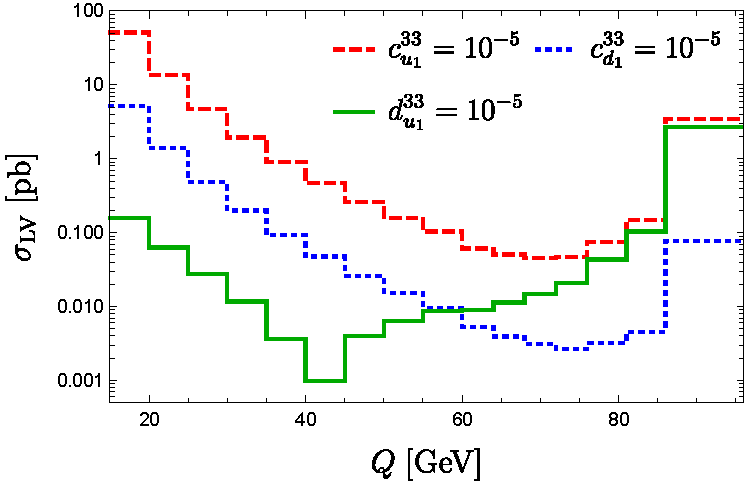
\includegraphics[scale=0.80]{figs/intro_theory/coeff_bounds.pdf}
\caption{
Order-of-magnitude estimates of sensitivity to laboratory
Standard-Model Extension (SME) coefficients as a function of $Q$ from predictions in 
Ref.~\cite{Lunghi_2021}. The $y$-axis
displays the Lorentz-violating contribution
to the total cross section in picobarns as
a function of invariant mass $Q$ from three
coefficients, $c_{u_1}^{33}, c_{d_1}^{33}$ and 
$d_{u_1}^{33}$ fixed to $10^{-5}$. 
The subscripts $u_1, d_1$ denote
the first-generation quarks, $u,d$. The superscripts
33 denote the 33-component of 
$c^{\mu\nu}_{u_1}$, etc. It is observed that the $c$-type coefficients
have most sensitivity to low $Q$ while the $d$-type
coefficient has most sensitivity on the $Z^0$ pole
at $Q = m_Z$. 
}
\label{fig:coeff_bounds}
\end{figure}


\clearpage
\section{Theoretical background} %% [Nathan / Enrico]
\label{lab:Theory}
\subsection{The motivation for and structure of realistic LIV}
\label{ssec:LV}
%
%
The absence of a predictive theory of quantum gravity
with accompanying low-energy signals
remains an open problem. Early work in
string theory demonstrated that 
if additional tensor-valued fields $T^{\mu\nu\cdots}$
obtained a nonzero vacuum expectation value (vev)
this could lead to the spontaneous violation of 
Lorentz and CPT symmetry~\cite{Kostelecky:1988zi,Kostelecky:1991ak}. 
These vevs would generate additional interactions
in an effective fermion theory at low energies 
with schematic form~\cite{Kostelecky:1991ak}
%
\begin{equation}
\label{lowE}
\mathcal{L}_{\text{LV}} \sim 
\frac{\lambda}{M^{k}}\braket{T}\cdot
\bar{\psi}\Gamma(i\partial)^{k}\psi+ \text{h.c.},
\end{equation}
%
where $\lambda$ is a coupling constant, 
$M$ is the scale of new physics 
(perhaps, but not necessarily, the Planck scale), $k$ is a positive 
integer and $\braket{T} \equiv \braket{T^{\mu\nu\cdots}}$ 
represents tensor-valued vev contracted with the gamma-matrix
structure $\Gamma$ (with suppressed Lorentz indices) in 
the fermion bilinear product to its right, and h.c. stands
for Hermitian conjugation. 
The vev $\braket{T}$ breaks the four-dimensional Lorentz
invariance because it has Lorentz indices 
which ``point" in some direction. 
Experiments with sufficient sensitivity to measure the 
combination $\lambda \braket{T}/M^k$ could 
indirectly probe certain classes of string theories.
%This scenario contrasts with that of the SM Higgs mechanism, 
%where the associated vev $\sim \braket{\phi} = v \neq 0$ is simply a scalar.

Sustained interest in the possibility
of Lorentz violation as a realistic 
low-energy signal of Planck-scale
physics has come from other string-based approaches
\cite{Ellis:2008gg,Gliozzi:2011hj,Hashimoto:2012ig}, 
loop quantum gravity \cite{Gambini:2014kba,Rovelli:2010ed}, 
noncommutative field theories \cite{Carroll:2001ws,Carlson:2001sw,
Calmet:2004ii,Calmet:2004dn,Bailey:2018ifc}, 
high-energy electrodynamics and cosmic rays \cite{Carroll:1989vb, 
Coleman:1998ti}, and modified theories of gravity
\cite{Kostelecky:2020hbb,Kostelecky:2021xhb,
Kostelecky:2021tdf,deRham:2014zqa,Horava:2009uw,
Bluhm:2004ep,Bluhm:2007bd,Bluhm:2014oua}. Here we use
the adjective ``realistic" in the sense of those high-energy mechanisms/models
generating LIV that map onto low-energy effective field theories 
with desirable properties including energy-momentum conservation, 
locality, the SM gauge structure, etc., except 
(particle) Lorentz and CPT invariance. We work at the level of realistic
effective field theory and do not assume any particular 
high-energy mechanism inducing LIV.

LIV terms like~\eqref{lowE} have some unconventional properties
that are best understood by example.
Consider the following term:
\begin{equation}
\label{bterm}
\mathcal{L}_b = -b_\mu \bar \psi \gamma_5\gamma^\mu \psi.
\end{equation}
Here, the coefficient $b_\mu = (b_0,b_j)$ may be thought of as a vector vev.
Comparing $\mathcal{L}_b$ to the generic $\mathcal{L}_{\text{LV}}$ in 
Eq.~\eqref{lowE} shows that $b_\mu \leftrightarrow 
\lambda \braket{T}/M^0 =  \lambda \braket{T}$
and $\Gamma(i\partial)^0 \leftrightarrow \gamma_5\gamma^\mu$. 
In natural units, power counting indicates the 
mass dimension of the coefficient is $[b_\mu] = $\; GeV. As the Lorentz
index $\mu$ is contracted, $\mathcal{L}_b \rightarrow \mathcal{L}_b$ is invariant under Lorentz
transformations of the coordinate system, known as observer Lorentz transformations~\cite{ck97}.
If, in contrast, the \textit{physical system} $\psi$ is rotated, boosted, or some combination of both
while leaving the coordinates unaffected, 
then generically $\mathcal{L}_b \not\rightarrow \mathcal{L}_b$. 
This is known as a particle Lorentz transformation.
Under a particle transformation, $b_\mu \rightarrow b_\mu$, but
$\psi(x)$ transforms 
in general to a different field $\psi'(x)$ 
evaluated at the same spacetime point $x$. Thus, 
the full term ${\cal L}_b$ transforms to a distinct term
$\mathcal{L}'_b \neq \mathcal{L}_b$.
The reason $b_\mu$ is unaffected by particle transformations
is because it can be viewed as a 
background vector-valued field at 
every point in the vacuum, analogous
to the SM Higgs scalar background but including an orientation.
Terms like Eq.~\eqref{bterm} therefore only describe Lorentz-violating 
effects associated to the noninvariance under 
particle Lorentz transformations. 
To reiterate, ${\cal L}_b$ is invariant under observer transformations.
This is a desirable feature, because coordinate choices (i.e. changes
in the observer's perspective) 
are arbitrary---they should not affect the physics.
The ability to distinguish between particle and observer transformations
implies Lorentz invariance is violated. 

Equation~\eqref{bterm} also describes a 
CPT-violating effect because $\bar \psi \gamma_5\gamma^\mu \psi \rightarrow
-\bar\psi \gamma_5\gamma^\mu \psi$ under the operation of CPT and $b_\mu\rightarrow b_\mu$
because the CPT operation is necessarily a type of particle transformation. 
Thus, ${\cal L}_b \rightarrow -{\cal L}_b$ under a CPT transformation and is therefore CPT odd.

The equations of motion of a system follow from the Euler-Lagrange equations.
Performing particle transformations can change the
Lagrange density of terms like ${\cal L}_b$ in a nontrivial way. Thus, the system $\psi$ can experience
different equations of motion depending on its relative orientation to the background
field $b_\mu$. For example, one could perform a measurement where the laboratory apparatus
(containing the particle content associated to $\psi$) is initially upright. 
A second measurement could then be performed except with an
the apparatus in a horizontal position. By comparing the two measurements 
one could, in principle, infer the existence of $b_\mu$. This general idea will
be expounded upon when we discuss sidereal oscillations 
of event observables in the following subsections. 
%
%
\subsection{Standard-Model Extension (SME)}
\label{ssec:SME}
%
%
The Lagrange density ${\cal L}_b$ in Eq.~\eqref{bterm} is actually one
among many that appear in the model-independent 
effective field theory~\cite{Weinberg:2009bg} for Lorentz 
and CPT violation, known as the Standard-Model Extension (SME)
~\cite{ck96,ck98}. By construction, the SME provides a
model-independent parameterization
of all possible Lorentz-violating effects
constructed from SM and gravitational fields.
Each term in the SME can be thought of as
the product of a coefficient
for Lorentz violation
\footnote{For brevity 
we collectively refer to the 
coefficients for Lorentz (and possibly) CPT 
violation as ``SME coefficients". The SME coefficients
are sometimes called Wilson coefficients, given
they appear in an effective field theory. We refrain 
from using this latter terminology to avoid 
confusion with it usage in Lorentz-invariant effective
field theories.} 
of mass dimension $4-d$
with a Lorentz-violating field operator of dimension $d$.
For example, in ${\cal L}_b$ the coefficient for Lorentz violation is $b_\mu$
and the Lorentz-violating field operator is $-\bar\psi \gamma_5\gamma^\mu \psi$.
Because this field operator is mass dimension $d=3$, the coefficient for
Lorentz violation is of mass dimension $4-3=1$, as claimed.
CPT violation is also parametrized by the SME,
since for local and unitary quantum field theories,
when CPT invariance is violated, so too
is Lorentz invariance~\cite{ck97,owg}.
All SME terms violate Lorentz invariance, but the general pattern is
that those coefficients with odd numbers
of Lorentz indices also violate CPT invariance\footnote{This is true in the vast majority
of cases. There are two known exceptions,
but these cases involve SME coefficients which are irrelevant
for our study.}.

Our program will be based on the conservative approach of the SME. The SME
Lagrange density can be written as 
%
\begin{equation}
\label{SMEaction}
{\cal L}_{\text{SME}} = {\cal L}_{\text{SM}} + \delta {\cal L}_{\text{LV}},
\end{equation}
%
where ${\cal L}_{\text{SM}}$ is the SM Lagrange density 
and $\delta{\cal L}_{\text{LV}}$ represents all possible 
Lorentz-violating terms consistent with the SM field content and
$SU(3)\times SU(2)\times U(1)$ gauge structure. Experimental results
suggest it is reasonable to take $\delta{\cal L}_{\text{LV}}$ as
perturbations with respect to ${\cal L}_{\text{SM}}$. This is equivalent
to saying the coefficients for Lorentz violation are treated as perturbative
quantities with respect to the mass scales appearing in the process of interest. 

SME operators of mass dimension $d\leq 4$ 
are power-counting renormalizable and part of the \textit{minimal} SME.
There are a finite number parameters in the minimal SME. This is the theory
obtain by taking the SM and relaxed the conditions
of particle Lorentz and CPT invariance.
In contrast, operators with $d>4$ are power-counting nonrenormalizable and infinite
in number. They are part of the \textit{nonminimal} SME. Just as with 
Lorentz invariant nonrenormalizable theories like the Standard Model Effective
Field Theory (SMEFT), the nonminimal SME takes on a particular importance
in high-energy process like collider processes. Our program considers
both minimal and nonminimal SME effects. 

To summarize, the SME provides a rigorously justified
analysis framework for probing
generic Lorentz- and CPT violating effects
in experiments. This is evidenced by the hundreds 
of constraints placed using the SME over the past two decades~\cite{datatables}.
Despite the impressive progress, some
sectors of the SME, including the quark- and electroweak
sectors, remain largely unexplored.
In the proceeding sections, we describe recent progress
on this front and the role existing
ATLAS Drell-Yan measurements will play in expanding the 
search for Lorentz violation.
%
%
\subsection{Summary of SME studies involving quarks, gluons, and hadrons}
\label{ssec:prevstudies}
%
%
Briefly reviewing existing studies involving 
Lorentz-violating effects in quarks and gluons (partons) 
and hadrons puts our search into context.

Beginning at the lowest mass dimension $d = 3$, 
``$a$-type" effects $-a_\mu \bar\psi \gamma^\mu \psi$ 
have been constrained over a range of ten orders 
$\lesssim 10^{-12}$-$10^{-22}$\;GeV from 
$K, D, B_d$, and $B_s$ meson oscillations, and
from mapping quark-level coefficients to meson-level effective
coefficients using chiral perturbation theory ($\chi$PT)
~\cite{Kostelecky:1997mh, Kostelecky:1999bm, Kostelecky:2000ku, 
Isgur:2001yz, Nguyen:2001tg, Babusci:2013gda, Kostelecky:2001ff, 
Aubert:2007bp, Kostelecky:2010bk, Abazov:2015ana, 
Aaij:2016mos, Roberts:2017tmo, Schubert:2016xul,Altschul:2019beo}. 
Similar techniques have led to $d=5$ constraints 
on $K, D, B_d$, and $B_s$ meson 
effects~\cite{Edwards:2018lsn, Edwards:2019lfb}. 
The combination of $\chi$PT with 
astrophysical measurements have produced
various levels of sensitivity to 
$d=4$ ``$c$-type" effects $c_{\mu\nu}\bar\psi i\partial^\mu\gamma^\nu \psi$ 
on light quark ($u$, $d$) coefficients and 
``$k$-type" gluon effects 
$-\tfrac{1}{4}k^{\mu\nu\alpha\beta}G^{a}_{\mu\nu}G^{a}_{\alpha\beta}$, respectively
~\cite{Kamand:2016xhv,Kamand:2017bzl,Altschul:2019beo,
Noordmans:2016pkr,Noordmans:2017kji}. 
Similar constraints on light quarks 
have been placed considering 
the absence of photon decay 
and vacuum Cherenkov radiation 
\cite{Gagnon:2004xh, Altschul:2006uw, Kostelecky:2013rta, Schreck:2017isa}. 
Constraints on heavy quarks (the second and third generation)
are few in comparison and are typically
substantially weaker than those on light quarks. 
A few bounds have resulted from LEP 
data~\cite{Karpikov:2016qvq}, 
$t\bar t$ production at Fermilab 
and the LHC~\cite{Berger:2015yha,Abazov:2012iu,Carle:2019ouy},
radiative corrections to the photon propagator~\cite{Satunin:2017wmk}, 
and potentially stable top-flavored hadrons~\cite{Altschul:2020wkw}

%Colliders operate in the 
%$\sim 10^2$-$10^4$\;GeV range
%are situated between the typically $\sim$ eV-MeV range 
%of low-energy experiments
%involving atomic, mesonic and baryons systems 
%and that of the most energetic cosmic rays observed, which  
%exceed LHC energies by over 7 orders of magnitude. 
%Despite the substantial reduction in energy over
%cosmic-ray observations 
A number of leading constraints in the electron
and photon sectors have been placed with collider data. 
However, these constraints are limited to the
rotationally invariant combinations 
of the SME coefficients~\cite{Altschul:2009xh,Altschul:2010na,kl19}.
Most of the SME coefficients are not rotationally invariant.
Colliders have some advantages over other experiments
in constraining the larger set of rotation-violating subsets 
of SME coefficients. These advantages include
the large number of events collected semi-regularly
over long durations (many months to years). 
%and control over colliding beamlines. 
These features make collider experiments suitable for 
\textit{sidereal analyses}, which track the oscillation of
an observable as a function of the Earth's 
sidereal period $\sim$ 23 hrs 56 mins. 
This technique was utilized in Ref.~\cite{Abazov:2012iu}
to place the constraints on several components 
of the top-quark $c$- and $d$-type 
coefficients (see the following subsection).

Advances in theory and phenomenology (by
theory STA members of our program)
have enabled arbitrary-dimension $d$
quark-sector effects to be incorporated in
perturbative hadronic process, in particular
deep inelastic scattering and the Drell-Yan process 
~\cite{Kostelecky:2016pyx, Lunghi:2018uwj, Kostelecky:2019fse,lssv21}. 
We note that gauge-sector Lorentz violation (e.g. involving Lorentz-violating effects
in the $Z$ boson itself) have also
been considered in Refs.~\cite{Fu:2016fmf, Colladay:2017zen, Michel:2019tti}, 
though these considerations lie outside our current goals.

Focusing on the developments in
Refs.~\cite{Kostelecky:2016pyx, Lunghi:2018uwj, Kostelecky:2019fse,lssv21}, 
we show that ATLAS data of Drell-Yan 
events on the $Z$-boson pole result 
in first constraints on the chiral ``$d$-type" coefficients, 
which are particularly challenging to probe, 
and derive competitive constraints on
the $c$-type coefficients (introduced above). 
%
%
\subsection{Minimal quark-sector effects}
\label{ssec:canddtype}
%
%
Our primary interest is to investigate the leading
quark-sector effects\footnote{By ``leading" we mean those SME operators
of most relevance to the considered process of dilepton production. 
%For more information see Sec.~\ref{ssec:theorydetails}.
}.
They are given by three terms in the quark sector of the SME:
%
\begin{align}
\label{model1}
\mathcal{L} &= \tfrac{1}{2}i c_{Q_i}^{\mu\nu}\overline{Q}_i\gamma_\mu\overset{\text{\tiny$\leftrightarrow$}}{D}_\nu Q_i  
+ \tfrac{1}{2}i c_{U_i}^{\mu\nu}\overline{U}_i\gamma_\mu\overset{\text{\tiny$\leftrightarrow$}}{D}_\nu U_i 
 + \tfrac{1}{2}i c_{D_i}^{\mu\nu}\overline{D}_i\gamma_\mu\overset{\text{\tiny$\leftrightarrow$}}{D}_\nu D_i \;,
\end{align}
where $D_\nu$ is the conventional (SM) covariant derivative. 
The fields have the usual definitions
\begin{align}
Q_i = \begin{pmatrix} u_i \\ d_i \end{pmatrix}_L, \quad U_i = \left(u_i\right)_R, \quad D_i = \left(d_i\right)_R.
\end{align}
%
The index $i = 1, 2, 3$ denotes flavors $u_i = (u, c, t)$ and 
$d_i = (d, s, b)$ and the SME coefficients are given 
by $c_{Q_i}^{\mu\nu}$, $c_{U_i}^{\mu\nu}$, and $c_{D_i}^{\mu\nu}$. 
They may be taken as symmetric and traceless matrices, leaving
nine independent components per type $Q, U, D$. 
It is customary and useful to define the combinations
%
\begin{align}
\label{eq:quarkcoeffs}
c_{u_i}^{\mu\nu} &= (c_{Q_i}^{\mu\nu} + c_{U_i}^{\mu\nu})/2, \quad c_{d_i}^{\mu\nu} = (c_{Q_i}^{\mu\nu} + c_{D_i}^{\mu\nu})/2  \;, \nonumber\\
d_{u_i}^{\mu\nu} &= (c_{Q_i}^{\mu\nu} - c_{U_i}^{\mu\nu})/2, \quad d_{d_i}^{\mu\nu} = (c_{Q_i}^{\mu\nu} - c_{D_i}^{\mu\nu})/2  \;,
\end{align}
%
with the constraint $c_{u_i}^{\mu\nu} -c_{d_i}^{\mu\nu} 
= d_{d_i}^{\mu\nu} - d_{u_i}^{\mu\nu}$. As suggested by the subscripts, 
we refer to these latter coefficients as the $c$- and $d$-type coefficients. 
When expressing the Lagrange density~\eqref{model1} in terms of mass eigenstates, 
the $d$-type coefficients are contracted with a Lorentz-violating operator
$\bar\psi(i\partial_\mu)\gamma_5\gamma_\nu \psi$ and therefore are
associated with a chiral current. 
%
%
\subsection{LIV effects in the Drell-Yan process}
\label{ssec:LIVDY}
%
%
Direct probes of the $c$- and $d$-type coefficients 
are typically frustrated by QCD confinement. However, 
perturbative QCD factorization is known to be maintained
in the presence of these coefficients. Analytical
results for the scattering cross sections
are thus possible and are available for analysis. 
%
The $d$-type coefficients introduce additional
complications relative to the $c$-type coefficients.
In contrast to the $c$-type coefficients, the 
$d$-type coefficients modify the polarization properties of quarks.
It turns out this makes them significantly harder to probe. 
For example, the presence of virtual gluons inside
a hadron imply a given quark
does not have a well-defined spin.
For a spin-zero meson, the net spin from 
valence quarks must 
average to zero. This means that even if the 
$d$-type effects are present
they average to zero and are unobservable 
in spinless mesons like pions. 
%
It has also been emphasized~\cite{ls18} that 
unpolarized hadronic processes
mediated by a photon or gluon
are also insensitive to $d$-type
coefficients, due to the opposite-sign 
contributions in the scattering amplitudes.

The only known ways to probe the $d$-type coefficients
are with unpolarized beams exchanging a $W$ or $Z$ boson,
or though polarized beamlines. Since no currently operating
colliders fall into the latter category, this leaves
the LHC as the sole experiment 
for probing the $d$-type coefficients. 

%% One alternative is to consider polarized beamlines,
%% however no existing collider is 
%% relevant in this context. In contrast, 
%% for electroweak-mediated processes there
%% \textit{is} the possibility to probe the
%% effects of the $d$-type coefficients, 
%% due to the inequality of left- and right-handed
%% couplings to the $Z,W^{\pm}$~\cite{lssv21}. 
%% This method is the only known possibility to independently
%% and directly probe the $d$-type quark coefficients
%% with existing collider data. The Drell-Yan process
%% is a perfect candidate signal because 
%% data exists in the invariant mass region where
%% the $Z$-boson goes on shell, which is also where sensitivity
%% to the $d$-type coefficients are maximal.
%% In contrast, for a similar process like deep inelastic scattering,
%% the exchanged $Z$ relative to photon $t$-channel exchange is greatly 
%% suppressed. 
With regard to the
$c$-type coefficients, the bounds
we expect to obtain~\cite{ls18,klsv19}
will not be competitive with existing 
first-generation limits. However, we will also 
probe distinct linear coefficient combinations and
the second-generation ($s,c$). The latter
constraints will exceed the few existing ones by 
by a two or so orders of magnitude~\cite{Karpikov:2016qvq}.
As suggested, the $d$-type coefficients are the most 
motivated and uniquely suitable for study
using ATLAS data of the Drell-Yan process 
on the $Z$-boson pole.
%
%
\subsection{Dilepton distribution}
\label{ssec:DYxsec}
%
%
This section summarizes the cross section calculations relevant
for our analysis and described in Refs.~\cite{Kostelecky:2019fse,lssv21}.
%It is emphasized that 
%unpolarized DY process in the ultrarelativistic limit, through $\gamma/Z$ 
%interference and pure $Z$ exchange, provides a natural avenue for 
%accessing and constraining these coefficients. Note that effects 
%of Lorentz violation on the $Z$ boson have also been studied 
%in similar processes \cite{Fu:2016fmf, Colladay:2017zen, Michel:2019tti}, 
%however, these considerations are outside the scope of this work. 
%The leading-order cross section as a function of 
%the dilepton invariant mass is derived.  Coupled with data on $Z$-boson 
%production from the LHC, real and simulated constraints are 
%placed on the coefficients for Lorentz violation for $u, d, s,$ and $c$ quarks
%
%

The leading-order Drell-Yan dilepton distribution
$d\sigma/dQ^2$ including photon, 
photon-$Z$ interference, and pure $Z$ exchange including 
the effects from Eq.~\eqref{model1} is \footnote{Recalling the assumption that the LIV effects are small relative to the SM contributions, we work at 
first-order in the SME coefficients, disregarding 
the highly suppressed quadratic (and all higher-order) corrections.}\footnote{Note this is Eq. (3.14) in Ref.~\cite{lssv21}, except here
the prefactor for the interference term now correctly
reads $+(1-4\sin^2\theta_W)/4$, whereas the Ref.~\cite{lssv21}
has the typos $-(1+4\sin^2\theta_W)/12$.}
%
\begin{align}
\label{DYsigmadQ2}
&\frac{d\sigma}{dQ^2} =  \frac{4\pi\alpha^2}{3 N_c}
\sum_f \left[\frac{e_f^2}{2Q^4} +\frac{1-m_Z^2/Q^2}{(Q^2 -m_Z^2)^2 + m_Z^2\Gamma_Z^2} 
\frac{1-4\sin^2\theta_W}{4\sin^2
\theta_W\cos^2\theta_W}e_fg_{fL}  \right. \nonumber\\
&\left. + \frac{1}{(Q^2 -m_Z^2)^2 + m_Z^2\Gamma_Z^2}
\frac{1+(1-4\sin^2\theta_W)^2}{32\sin^4\theta_W\cos^4\theta_W}g_{fL}^2\right]
\int_{\tau}^1 dx\frac{\tau}{x}\widehat{\sigma}'_{f}
\left(x,\tau/x,c_{fL}^{\mu\nu}\right) + (L\rightarrow R),
\end{align}
%
where the number of colors $N_c = 3$, $m_Z$ and $\Gamma_Z$ are $Z$ boson mass and width, 
$e_f = \{2/3,-1/3,-1/3,2/3\}$
is the fractional quark charge for flavor $f = \{u,d,s,c\}$, and 
the left and right chiral couplings are $g_{fL} = I_W^{(3)}-e_f\sin^2\theta_W$, 
$g_{fR} = -e_f\sin^2\theta_W$.
The Drell-Yan scaling variable is $\tau \equiv Q^2/s$ and 
%
\begin{align}
\label{sigmaprime}
\widehat{\sigma}'_{f}\left(x,\tau/x, c_{fL}^{\mu\nu}\right) 
&\equiv \left( 1+ \frac{2}{s}
c_{fL}^{\mu\nu}(1+x^2/\tau)(p_{1\mu}p_{1\nu}+ p_{1\mu}p_{2\nu}
+ (p_1\leftrightarrow p_2))\right)  f_{f\text{S}}(x,\tau/x) \nonumber\\
&\quad +  \frac{2}{s}c_{fL}^{\mu\nu}\left(xp_{1\mu}p_{1\nu} 
+\frac{\tau}{x}p_{1\mu}p_{2\nu} + 
(p_1\leftrightarrow p_2) \right) f'_{f\text{S}}(x,\tau/x), 
\end{align}
%
where the flavor-symmetric PDF products are defined as
%
\begin{align}
&f_{f\text{S}}(x,\tau/x) \equiv f_{f}(x)f_{\bar f}(\tau/x) +  f_{f}(\tau/x)f_{\bar f}(x), \label{PDFprodf}\\
&f'_{f\text{S}}(x,\tau/x) \equiv f_{f}(x)f'_{\bar f}(\tau/x) +  f'_{f}(\tau/x)f_{\bar f}(x). \label{PDFprodbarf}
\end{align}
%
The first, second, and third terms 
in the brackets in Eq.~\eqref{DYsigmadQ2}
are associated with the electromagnetic, 
interference, and $Z$-exchange contributions, respectively. Note that
$d\sigma/dQ^2$ is a Lorentz observer scalar. It can thus be evaluated
in any observer frame. In whatever frame is chosen, the SME coefficients
are those expressed in that frame. 
Application to ATLAS dilepton data means the ATLAS detector frame 
is the relevant observer frame. 
This frame will be discussed in detail in the following subsections.
%
%
\subsection{Sidereal signals, the Sun-Centered frame, and the ATLAS detector frame}
\label{ssec:sidereal}
%
%
Fundamental physical laws imply equations
of motion for particles and 
fields that are valid in inertial frames.
However, experiments are typically
described with Earth-based coordinate 
systems. These are nonintertial frame, primarily 
due to the Earth's rotation. 
Noninertial effects like the
centrifugal force $F_{\text{c}} = m\omega^2 r$
are usually several orders of magnitude smaller than the
gravitational force $F_{\text{g}} \simeq mg$. As $F_g$
is considerably weaker than the electroweak 
and strong forces at the scale
of collider experiments, noninertial
effects are safe to neglect. 

Noninertial effects cannot be disregarded in the presence of LIV.
Because the Earth is rotating, 
the orientation of the laboratory with respect to the SME coefficients,
which may be viewed as background tensor fields, changes with time.
The dominant contribution to this time variation 
comes from the Earth's axial rotation.
This will produce oscillations at harmonics of the Earth's sidereal frequency 
$\omega_\oplus = 2\pi/(\text 23\; \text{hr}\; 56\; \text{min}\; 4.091\; \text{sec})$
in laboratory observables.
Furthermore, as no two experiments (in principle)
have identical coordinates and measurement apparatus orientations,
every experiment is sensitive to a unique linear combination of background effects. 

For a straightforward comparison of results from distinct experiments, it is
useful to introduce a fixed and nonrotating inertial frame. To a good approximation,
the SME coefficients can be taken as fixed in this frame~\cite{ak04}. 
The commonly adopted frame for SME analyses is the 
Sun-centered Frame (SCF)~\cite{kd16,km02,k2000,klv17,ls18,km09}, 
which we describe in detail.

Expressing laboratory observables
in terms of coefficients defined 
in the SCF introduces explicit time dependence.
The explicitly time-dependent laboratory coefficients
are re-expressed in terms of the constant SCF coefficients 
at the cost of introducing sinusoidal functions of the sidereal phase. 

The SCF spatial axes $X^J \equiv (X, Y, Z)$ are
centered on the Sun such that 
the $Z$ axis is parallel to the Earth's rotation axis, 
the $X$ axis points toward the 2000 vernal equinox, 
and the $Y$ axis completes a right-handed coordinate system (see Fig.~\ref{fig:scf}).
Analogously, the time coordinate of the SCF is denoted $T$.
The spacetime coordinates of the SCF are then $X^\mu = (T,X^J)$.
As the definitions would suggest, the time $T=0$ is chosen to coincide 
with the date and time of the 2000 vernal equinox. 
We identify the 2000 vernal equinox as occuring
on March 20th, 2000 at 7:35 am Universal Coordinated time (UTC).

In the following few subsections we introduce a number of frames and coordinate
transformations that taken together will connect the SCF to the ATLAS detector frame.
The net transformation will allow us to reexpress the time-dependent ATLAS frame 
SME coefficients in terms of the constant SCF coefficients. 
%
\begin{figure}[ht]
\centering
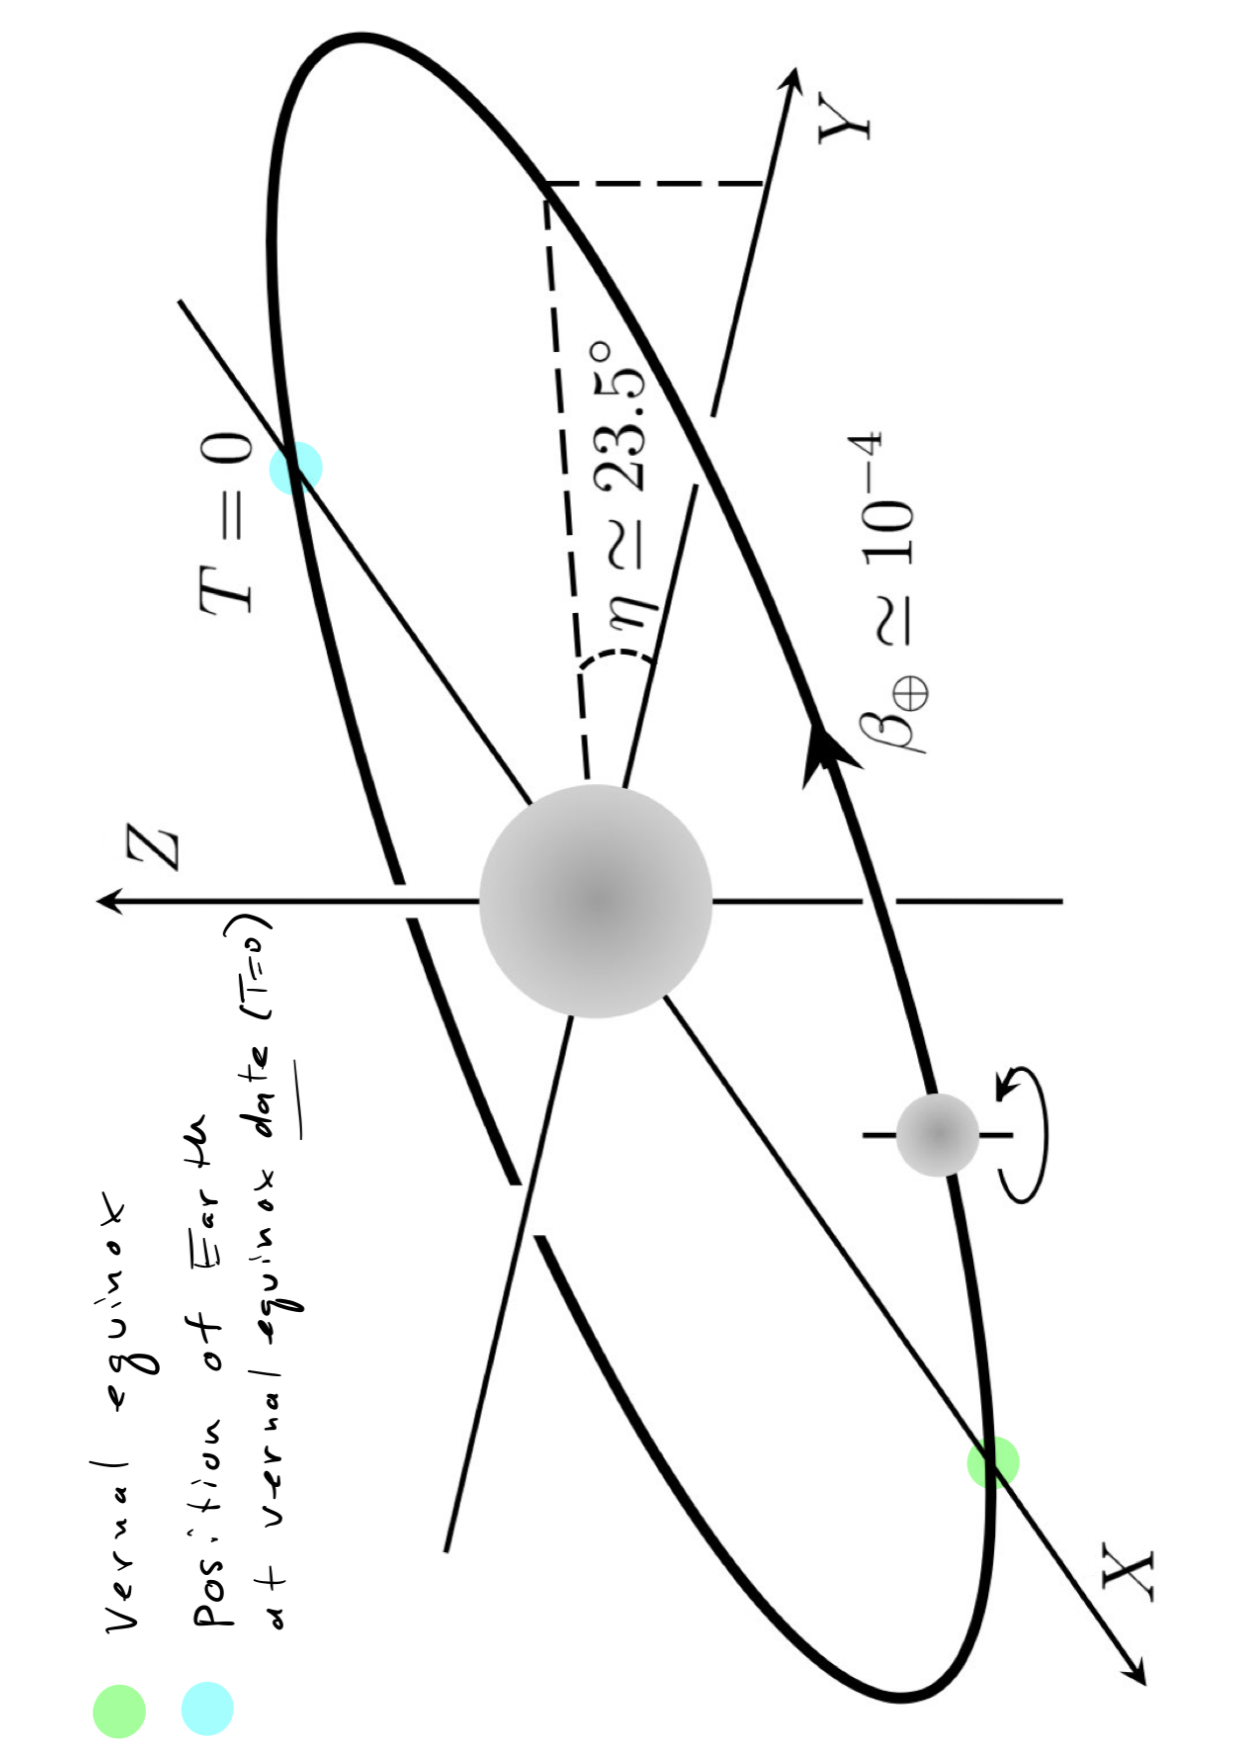
\includegraphics[scale=0.50,angle=-90]{figs/intro_theory/SCF_pic.pdf}
\caption{Edited illustration of the SCF (originally image from Ref.~\cite{kd16}). 
The Sun is the larger shaded disk in the center and
and the Earth the smaller disk revolving about the Sun. 
When looking down the Sun $Z$ axis, the Earth
is seen revolving counterclockwise in an approximately circular orbit 
and rotating counterclockwise about its rotation axis. 
The SCF axes are chosen such that $Z$ axis 
is parallel with the Earth's rotation axis. The orbit of the Earth
in this frame is inclined relative to the $X$-$Y$ plane
by $\eta \simeq 23.5^{\circ}$. 
The $X$-$Y$ plane is parallel to the
Earth's equatorial plane. The vernal equinox 
is the point where the $X$ axis intersects 
the Earth's orbit (green dot). On the date 
of the 2000 vernal equinox the Earth 
is positioned at the light-blue dot near $T=0$. 
At this latter dot, the $X$ axis intersects the Earth
and points from the Earth to the Sun.
At this moment, there is one position on the Earth's equator where an observer 
would see the Sun directly overhead (toward their local zenith)
at noon local time. The longitude of this location is given by $\lambda_0$
from Eq.~\eqref{angularshift}.}
\label{fig:scf}
\end{figure}
%
Next, the canonical frames used to describe the
laboratory apparatus frame and its connection
to the SCF are introduced.
%
%
\subsection{Standard laboratory frame}
%
%
The \textit{standard laboratory frame}
is a fixed frame on the surface of the Earth, and
hence rotates with respect to the SCF. 
The coordinates of this frame are 
defined as $x^j \equiv (x,y,z)$, where
the $x$ axis points toward local south, the $y$ axis toward
local east, and the $z$ axis toward the local zenith. 
%
It is convenient to identify the 
standard laboratory frame time coordinate $t$ 
with the local sidereal time $T_\oplus$.
The local sidereal time is defined to have 
an origin $T_\oplus = 0$ when the laboratory $y$ axis 
is parallel to the Sun $Y$ axis, $y||Y$. 

Under the approximation that the Earth moves in a circular
orbit around the Sun, the transformation from the 
SCF to the standard laboratory frame 
is given by a rotation $R^{jJ}$ such that 
%
\begin{equation}
x^j = R^{jJ}X^J,
\end{equation}
%
where the sum over the repeated index $J$ is implied.
To determine $R^{jJ}$, we imagine that the coordinates $x^j$ and
$X^J$ are initially parallel and with coincident origins. 
From the viewpoint of $X^J$,
the coordinates $x^j$ appear to be rotating.
So, first a rotation about the $Z$
axis by an angle $\omega_\oplus T_\oplus$ is performed:
%
\begin{equation}
R_{Z} = \begin{pmatrix} \cos\omega_\oplus T_\oplus 
& \sin\omega_\oplus T_\oplus & 0 \\ 
-\sin\omega_\oplus T_\oplus 
& \cos\omega_\oplus T_\oplus & 0 \\ 0 & 0 & 1 \end{pmatrix}.
\end{equation}
%
In looking down the $Z$ axis, the $x$ and $y$ axes will be rotating
counterclockwise in the $X$-$Y$ plane. 
This is consistent with the fact that
the Earth rotates counterclockwise about
its own axis when viewed from the northern hemisphere. 
Next, a second rotation is needed 
to make $\widehat{z}\cdot\widehat{Z} = \cos\chi$,
where $\chi$ is the colatitude of the 
standard laboratory\footnote{the hat notation indicates unit vectors}.
This is achieved by a counterclockwise 
rotation about the $Y$ axis by an angle $\chi$:
%
\begin{equation}
R_{Y} = \begin{pmatrix} \cos\chi & 0 & -\sin\chi \\ 
0 & 1 & 0 \\ \sin\chi & 0 & \cos\chi\end{pmatrix}.
\end{equation}
%
Thus, the net rotation is now $R^{jJ} = R_{Y}\cdot R_{Z}$ and given by
%
\begin{equation}
\label{RjJ}
R^{jJ} = \begin{pmatrix} \cos\chi\cos\omega_\oplus T_\oplus & \cos\chi\sin\omega_\oplus T_\oplus 
& -\sin\chi \\ -\sin\omega_\oplus T_\oplus & \cos\omega_\oplus T_\oplus & 0
\\ \sin\chi\cos\omega_\oplus T_\oplus & \sin\chi \sin\omega_\oplus T_\oplus & \cos\chi
\end{pmatrix}.
\end{equation}
%
Note this is Eq. (44) in Ref.~\cite{kd16}.
For more information on the 
standard laboratory frame, see Ref.~\cite{km02}. 
An illustration depicting the rotation~\eqref{RjJ} is 
given in Ref.~\cite{k2000}. 

Connecting other laboratory frames, 
such as the ATLAS detector frame, to the SCF can be achieved by 
applying additional rotations following $R^{jJ} = R_Y\cdot R_Z$ given in Eq.~\eqref{RjJ}.
%
%
\subsection{ATLAS detector frame}
%
We now describe additional rotations that must be performed to
connect the ATLAS frame to the SCF. 

Recall that the standard laboratory frame (positive) $y$ axis
points to local east.
At the ATLAS detector interaction point the collider ring
has its beamlines oriented at some angle $\psi$ north of east.
The following matrix rotates the $y$ axis to this direction:
%
\begin{equation}
\label{psirot}
\begin{pmatrix} \cos\psi & \sin\psi & 0 \\ 
-\sin\psi& \cos\psi& 0 \\ 0 & 0 & 1 \end{pmatrix}.
\end{equation}
%
Note that $y$ is now pointing along 
the ATLAS ``beamline 1" direction.
As is typically chosen, the beam-direction
axis is in the $\widehat{z}$ direction. A transformation
that swaps the $y$ and $z$ axes is 
%
\begin{equation}
\label{Rswap}
\begin{pmatrix} \pm 1 & 0 & 0
\\ 0 & 0 & 1 \\ 0 & \mp 1 & 0 
\end{pmatrix}.
\end{equation}
%
The upper (lower) signs orient $\widehat{z}$ antiparallel (parallel) 
to the prior $\widehat{y}$ direction. 
For either sign the final $\widehat{y}$ 
direction points toward the local zenith.
Applying Eqs.~\eqref{psirot},\eqref{Rswap} after
Eq.~\eqref{RjJ} results in the rotation used in studies involving the 
HERA/EIC colliders in \cite{klv17, ls18}. For ATLAS, 
one final transformation needed because the ATLAS detector 
is slightly inclined relative to the $\widehat{z}$
direction. Performing a rotation of $-\delta$ around the $\widehat{x}$
direction achieves 
this\footnote{Our conventions for rotations are that
a positive angle is associated with a counterclockwise rotation. Here
we have a clockwise rotation around the $x$ axis, hence the minus sign.}:
%
\begin{equation}
\begin{pmatrix} 1 & 0 & 0 \\ 0 & \cos(-\delta) & \sin(-\delta) \\ 
0 & -\sin(-\delta)& \cos(-\delta) \end{pmatrix}.
\end{equation}
%

In total, the net rotation converting 
the SCF coordinates to the ATLAS coordinates is found to be
%
\begin{align}
\label{Rnet}
R(T_\oplus) = \begin{pmatrix} 1 & 0 & 0
\\ 0 & \cos\delta & -\sin\delta \\ 0 & \sin\delta & \cos\delta
\end{pmatrix}&\begin{pmatrix} + 1 & 0 & 0
\\ 0 & 0 & 1 \\ 0 & - 1 & 0 
\end{pmatrix}
\begin{pmatrix} \cos\psi & \sin\psi & 0 \\ 
-\sin\psi& \cos\psi& 0 \\ 0 & 0 & 1 \end{pmatrix} \nonumber \\
&\times\begin{pmatrix} 
\cos\chi\cos\omega_\oplus T_\oplus & \cos\chi\sin\omega_\oplus T_\oplus 
& -\sin\chi \\ -\sin\omega_\oplus T_\oplus & \cos\omega_\oplus T_\oplus & 0
\\ \sin\chi\cos\omega_\oplus T_\oplus & \sin\chi \sin\omega_\oplus T_\oplus & \cos\chi
\end{pmatrix}.
\end{align}
%
The chosen sign in the $y\leftrightarrow z$ swap
matrix (Eq.~\eqref{Rswap}) identifies the 
beam $\widehat{z}$ direction with the ATLAS
``beam 2 direction"---see the ATLAS New Small Wheel TDR, Section 3.6.1, pg. 24.
The numerical values of the relevant angles are
%
\begin{align}
\label{angularvalues}
&\chi = 43.764290859^\circ, \\
&\psi = 168.7^\circ, \\
&\delta = |-\delta| = |-0.704^\circ| = + 0.704^\circ.
\end{align}
%
Note the minus sign in $\delta$ is taken into account in Eq.~\eqref{Rnet}.
For an expanded discussion of the SCF, standard
laboratory frame, and laboratory apparatus frame, see
Ref.~\cite{km09}.
%
%
\subsubsection{Explicit example}
\label{sec:phase_comp}
%
%
As a simple example, consider again our archetypal LIV effect:
${\cal L}_b = -b_\mu \bar \psi \gamma_5\gamma^\mu \psi$
from Eq.~\eqref{bterm}. Let us imagine we are working in the ATLAS detector frame.
Then $b_\mu = (b_0, b_j) $ has components decomposed 
in the coordinate basis describing this frame.
Noting Eq.~\eqref{Rnet}, we wish to express
$b_\mu$ in terms
of the fixed SCF frame coefficients, which we call
$b_{\text{SCF}}^\mu = (b^T, b^X, b^Y, b^Z)$.
Since the ATLAS detector and SCF differ by a coordinate 
transformation (Lorentz observer transformation), the 
coeffcient $b_\mu$ transforms like a usual four-vector:
%
\begin{align}
\label{blabSCF}
b^\mu = [R(T_\oplus)]^\mu_{\hphantom{\mu}\nu} b_{\text{SCF}}^{\nu},
\end{align}
%
where
$[R(T_\oplus)]^\mu_{\hphantom{\mu}\nu}$ is the four-dimensional
version of the spatial rotation matrix $R(T_\oplus)$ from Eq.~\eqref{Rnet}. 
The additional elements are $R^0_{\hphantom{0}0} = 1, 
R^0_{\hphantom{0}j} = R^j_{\hphantom{j}0} = 0$. 
As a simplifying limit, and 
without loss of generality, consider $\delta \rightarrow 0$. 
%
\begin{figure}[ht]
\centering
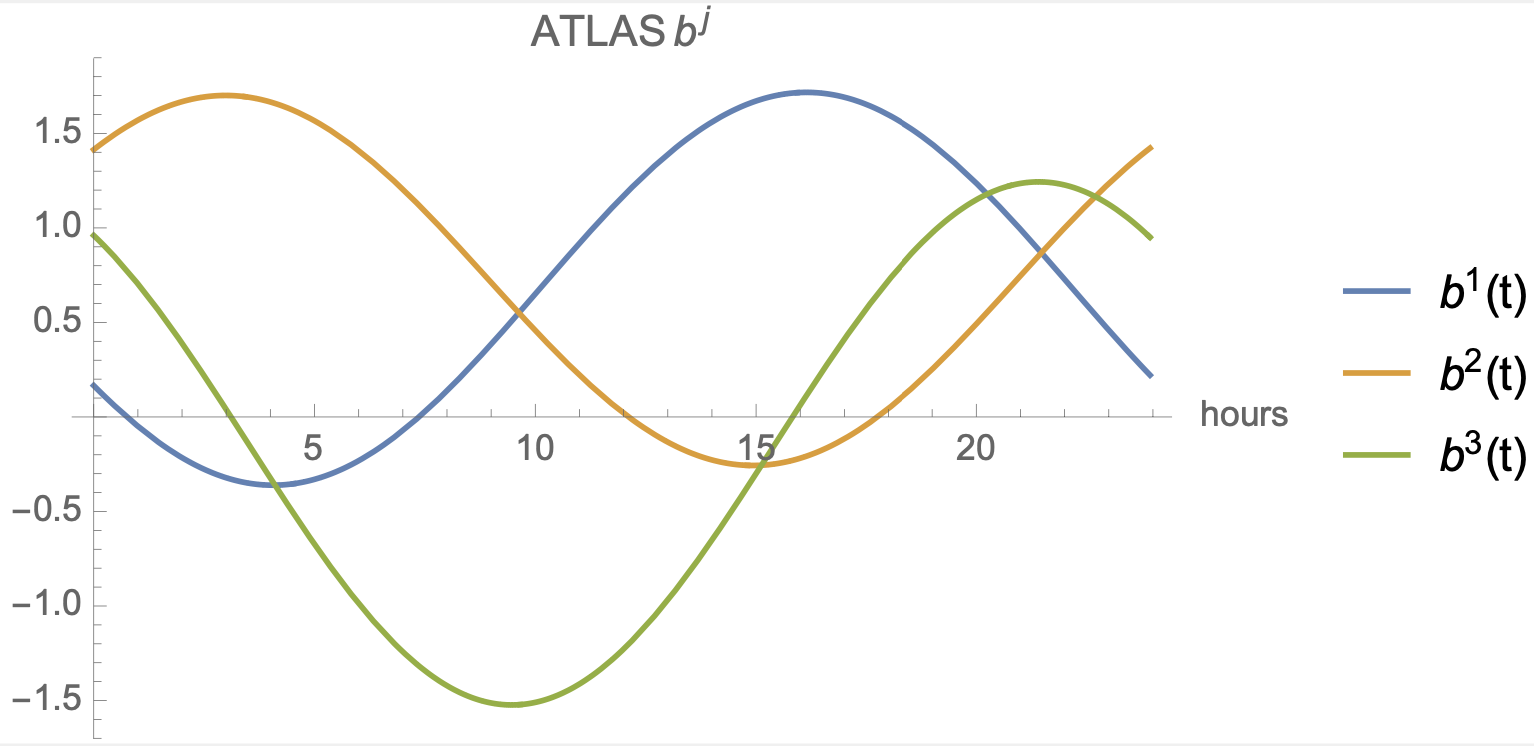
\includegraphics[scale=0.40]{figs/intro_theory/ATLASbj.png}
\caption{Components $b^j$ from Eq.~\eqref{ATLAScomps} 
plotted over a sidereal day for $b_{\text SCF}^J \equiv  1$. 
The (small) effects of setting $\delta = |-0.704^\circ|$ are also included.}
\label{fig:ATLASbj}
\end{figure}
%
It is then found that
%
\begin{align}
\label{ATLAScomps}
b^0 = \; & b^T \\
b^1 = \; & -b^Z\sin\chi\cos\psi + \cos(\omega_\oplus T_\oplus)(b^X\cos\chi\cos\psi + b^Y\sin\psi) \nonumber \\
      & + \sin(\omega_\oplus T_\oplus)(b^Y\cos\chi\cos\psi - b^X\sin \psi) \\
b^2 = \; & b^Z\cos\chi + b_X\cos(\omega_\oplus T_\oplus)\sin\chi + b_Y\sin(\omega_\oplus T_\oplus)\sin\chi  \\
b^3 = \; & -b^Z\sin\chi\sin\psi + \cos(\omega_\oplus T_\oplus)(b^X\cos\chi\sin\psi - b^Y\cos\psi) \nonumber \\
      \; & + \sin(\omega_\oplus T_\oplus)(b^Y\cos\chi\sin\psi + b^X\cos\psi)
%
%\begin{pmatrix} b^0 \\ b^1 \\ b^2 \\ b^3 
%\end{pmatrix} 
%= 
%\begin{pmatrix} b^T \\ -b^Z\sin\chi\cos\psi + \cos(\omega_\oplus T_\oplus)(b^X\cos\chi\cos\psi + b^Y\sin\psi)
%+ \sin(\omega_\oplus T_\oplus)(b^Y\cos\chi\cos\psi - b^X\sin \psi) \\
%b^Z\cos\chi + b_X\cos(\omega_\oplus T_\oplus)\sin\chi + b_Y\sin(\omega_\oplus T_\oplus)\sin\chi \\
%-b^Z\sin\chi\sin\psi + \cos(\omega_\oplus T_\oplus)(b^X\cos\chi\sin\psi - b^Y\cos\psi)
%+ \sin(\omega_\oplus T_\oplus)(b^Y\cos\chi\sin\psi + b^X\cos\psi)
%\end{pmatrix}.
\end{align}
%
We observe that the time dependence has been made explicit through
the functions $\cos(\omega_\oplus T_\oplus), \sin(\omega_\oplus T_\oplus)$. 
See Fig.~\ref{fig:ATLASbj}
for the resulting time dependence of the ATLAS 
components. Note that all
components have a distinct shape and that even
in the absence of time-dependent effects
there is a unique dependence on the laboratory location
through the angles $\chi, \psi$. 

For more complicated LIV backgrounds, like $c$- and $d$-type coefficients
introduced in Sec.~\ref{ssec:canddtype}, additional applications of the net rotation
matrix must be performed. For example,
%
\begin{equation}
\label{cuexample}
(c_{u_i})^{\mu\nu} = \left[R(T_\oplus)\right]^\mu_{\hphantom{\mu}\alpha}
\left[R(T_\oplus)\right]^\nu_{\hphantom{\nu}\beta}(c_{u_i})_{\text{SCF}}^{\alpha\beta},
\end{equation}
where the parentheses () have been introduced for clarity.
%
%
\subsubsection{Another explicit example}
\label{sec:phase_comp1}
%
%
We now revisit the cross section $d\sigma/dQ^2$ from Eq.~\eqref{DYsigmadQ2}.
It involves combinations of the coefficients
described in Eq.~\eqref{eq:quarkcoeffs}. Evaluation of $d\sigma/dQ^2$ in the
ATLAS detector frame reveals that the only time-dependent
coefficients that appear are $c_f^{33}, d_f^{33}$. We must re-express
these coefficients in terms of the SCF 
coefficients using, e.g., Eq.~\eqref{cuexample}. 
We find
%
\begin{align}
\label{c33}
c_{f}^{33} =&
\frac{1}{2}(c_{f}^{XX} + c_{f}^{YY})\left(\cos^2\chi\sin^2\psi + \cos^2\psi\right) +  c_{f}^{ZZ}\sin^2\chi\sin^2\psi
\nonumber\\
& - 2c_{f}^{XZ}\sin\chi\sin\psi
\left[\cos\chi\sin\psi\cos(\omega_{\oplus}T_{\oplus} )
+ \cos\psi\sin(\omega_{\oplus}T_{\oplus})\right]
\nonumber\\
& - 2c_{f}^{YZ}\sin\chi\sin\psi
\left[\cos\chi\sin\psi\sin(\omega_{\oplus}T_{\oplus})
- \cos\psi\cos(\omega_{\oplus}T_{\oplus})\right] \nonumber\\
& + c_{f}^{XY}\left[(\cos^2\chi\sin^2\psi - \cos^2\psi)\sin(2\omega_\oplus T_\oplus) - \cos\chi\sin(2\psi)\cos(2\Omega_\oplus T_\oplus)    \right] \nonumber \\
& +\frac{1}{2}(c_{f}^{XX} - c_{f}^{YY})\left[(\cos^2\chi\sin^2\psi - \cos^2\psi)\cos(2\omega_\oplus T_\oplus) \right. \nonumber\\
& \left.+ \cos\chi\sin(2\psi)\sin(2\omega_\oplus T_\oplus)\right],
\end{align}
%
and similarly for $d_f^{33}$. 
We see that the coefficients with SCF superscript 
indices $XX+YY$ and $ZZ$ are only associated to time-independent effects. 
Those with indices $XZ, YZ, XY, XX-YY$ introduce 
sidereal time-dependent effects and are of primary interest.
Inserting 
Eq.~\eqref{c33} into the laboratory-frame
expression of Eq.~\eqref{DYsigmadQ2} and
noting the constraint
%
\begin{equation}
c_{u_i}^{\mu\nu} - c_{d_i}^{\mu\nu} = d_{d_i}^{\mu\nu} - d_{u_i}^{\mu\nu},
\end{equation}
%
results in the observable of interest for our analysis.
%
%
\subsection{Initial conditions and shifts}
\label{sec:timeshift}
%
%
The previous sections focused on the spatial transformation from the 
SCF to the ATLAS detector frame and the implications for observables. 
In this section, we describe an important temporal transformation
that must be accounted for.

We begin by asking:
%
\begin{itemize}
\centering
\item[] \emph{Where on the equator at the vernal equinox 2000 ($T=0$)
is the Sun directly overhead (at noon local time)?}
\end{itemize}
%
At this location, the standard laboratory frame $z$ axis
is oriented such that 
$\widehat{z} \parallel \widehat{X}$, $\widehat{y} \parallel \widehat{Y}$, 
and $T = T_\oplus = 0$, assuming the origin of 
$T_\oplus$ is chosen to occur on the equinox date. This location
is found by noting there are 
$(4 + \frac{25}{60} \simeq 4.417)$ local hours that 
must elapse for the Sun to be approximately overhead at noon in the UTC 
timezone at longitude 0$^{\circ}$ (recall that the equinox
occurs at 7:35 am UTC). Therefore, the Sun
is overhead on the equator at a longitude \emph{advanced} by 
\begin{align}
\label{angularshift}
\lambda_0 &= 4.417\;\text{hr}\cdot\frac{2\pi}{24 \text{hr}}
\cdot\frac{180}{\pi} \nonumber\\
&= 66.25^{\circ},
\end{align}
which is in the Indian Ocean west of the Maldives, matching the claim 
in Ref.~\cite{kd16}. 
Note it is only at $\lambda_0$
that a (hypothetical) laboratory with $T = T_\oplus$ has its local zenith
pointing toward the Sun.

For a laboratory positioned at any other longitude, 
$\widehat{y} \parallel \widehat{Y}$ at an earlier
or later time than the equinox.  
Given the direction of Earth's rotation, 
for $\lambda < \lambda_0$, 
$T - T_\oplus > 0$, and for $\lambda > \lambda_0$, 
$T - T_\oplus < 0$. 
The time it takes for such laboratory to advance 
depends on a linear longitudinal shift,
and the time for $\widehat{y}$ to 
continually realign with $\widehat{Y}$ is a sidereal 
day with period 23 hr 56 min 4.091 s $\simeq$ 23.934 hr. 
This latter dependence on the sidereal day, 
as opposed to a 24-hour solar
day, is because the Earth is slightly changing
its angular position relative to the Sun
by an amount quantified by the sidereal day.
We find 
\begin{align}
\label{relation}
T - T_\oplus = \frac{\lambda_0 - \lambda}{360^{\circ}}\cdot 
(23.9344697\bar{2}\;\text{hr}),
\end{align}
which is Eq. (43) in Ref.~\cite{kd16} reported with higher precision. 
Note that this result is independent of the latitude of the laboratory. 
Also note that $T - T_\oplus$ can more generally depend
on a integer number $n$ of 
sidereal days, such that an 
additional shift $\frac{2\pi}{\omega_{\oplus}}n$
needs to be included on the right-hand side 
of Eq.~\eqref{relation} if the origin $T_\oplus = 0$ 
\textit{isn't} chosen on the 2000 vernal equinox date. 
%
As a relevant example, for ATLAS 
\begin{equation}
\lambda = 6.055279086^\circ,
\end{equation}
giving
\begin{align}
\label{TshiftATLAS}
T - T_\oplus\bigg|_{\text{ATLAS}} = 4.002\;\text{hr}.
\end{align}
Note that $2\times 10^{-3}\;\text{hr} = 7.28725\;\text{s}$. 
Thus, rounding to the nearest second, for the ATLAS 
experiment $\widehat{y}\parallel \widehat{Y}$ 
on March 20th, 2000 at 11:35:24 UTC.
It is this date and time 
that we identify with $T_\oplus\big|_{\text{ATLAS}} = 0$.
All data timestamps are assigned a 
unique $T_\oplus$ which is measured relative to this initial condition.
%
%\subsection{Example: $T_{\text Unix}$ comparison}

Since we have chosen to initialize our laboratory clock
with the local sidereal time, $t = T_\oplus$, 
every laboratory measurement comes with a time stamp $T_\oplus$.
However, suppose that events are instead known with 
respect to a different time origin, for instance
``Unix time", where $T_{\text{Unix}} = 0$ is defined as January 
1st, 0:00:00 UTC, 1970. To convert from Unix time to local time,
we must subtract off the difference
\begin{equation}
\label{Tshift}
(T_\oplus = 0) - (T_{\text{Unix} = 0}) = 953552124\;\text s
\end{equation}
from each event to compute how much time has elapsed since $T_\oplus = 0$. 
In Tab.~\ref{tab:datestimes} we 
compare the various dates and times discussed so far, as well as the sidereal
and solar phases with reference to $T_\oplus$ for ATLAS. 
%
\begin{table}
\centering 
\small
\begin{tabular}{c c c c c c c c} % centered columns (4 columns)
\hline\hline
event & calendar date & $T_{\text{Unix}}$
& $T$ & $T_\oplus$ & $\oplus\angle$ & $\odot\angle$ \\
%$\left(\frac{\mathcal{O}_{\rm SME}}{\mathcal{O}_{\rm SM}}-1\right)$  \\
\hline
1&$|$ 01/01/1970 00:00:00$|$& 0 $\qquad\qquad\hspace{.5mm}|$& -953537717
$|$& -953552124 $|$& 0.371415 $|$&  0.517083 \\
%
2&$|$ 01/01/2000 12:00:00$|$& 946728000 $\hspace{.5mm}|$& -6809717 $\quad|$& -6824124 $\quad|$& 0.35914 $\hspace{1.75mm}|$& 0.0170833\\
%
3&$|$ 20/03/2000 07:35:17$|$& 953537717 $\hspace{.5mm}|$& 0 $\qquad\qquad\hspace{1.0mm}|$& -14407 $\qquad|$& 0.857198 $|$& 0.833252\\
%
4&$|$ 20/03/2000 11:35:24$|$& 953552124 $\hspace{.5mm}|$& 14407 $\qquad\hspace{1mm}|$& 0 $\qquad\qquad\hspace{1mm}|$& 0 $\qquad\quad\hspace{1mm}|$& 0\\
%
5&$|$ 25/01/2021 18:49:42$|$& 1611600582$|$& 658062865  $\hspace{1mm}|$& 658048458 $\hspace{1mm}|$& 0.590071 $|$& 0.301597 \\
%
6&$|$ 25/03/2021 18:49:42$|$& 1616698182$|$& 663160465 $\hspace{1mm}|$& 663146058 $\hspace{1mm}|$& 0.117588 $|$& 0.301597 \\
\hline\hline 
\end{tabular}
\caption{Times other than the calendar date (GMT) are given in seconds. Sidereal ($\oplus\angle$) and solar ($\odot\angle$) phases are calculated
with respect to $T_\oplus$ for ATLAS.}
\label{tab:datestimes}
\end{table}
%
Alternatively, the bin for a given event $T_\oplus$ may be calculated from
\begin{align}
\text{bin \#} =  
\text{mod}\left[\frac{T_\oplus - \text{mod}[T_\oplus,\frac{2\pi}{n\omega_\oplus}]}
{\frac{2\pi}{n\omega_\oplus}},n\right] + 1, 
\label{eq:sid_phase_bin}
\end{align}
where $n$ is the number of bins (intervals) the sidereal day has been split into. For example, 
for $n=1$ the length of the interval is the sidereal day, which
is 23.94 hr. For $n=2$, there are two intervals of duration 23.94/2 = 11.97 hr, 
and so on. 



\subsection{Minimal SME coefficients probed in this analysis}
\label{subsec:WC}

As shown in Sec.~\ref{sec:phase_comp}, for a given flavor $f$
there are four coefficient types $XZ, YZ, XY, XX-YY$ that induce
sidereal time dependence in the Drell-Yan dilepton distribution 
$d\sigma/dQ^2$. In the basis of $c$- and 
$d$-coefficients (Eq.~\eqref{eq:quarkcoeffs}) there are
three independent coefficient types per generation. This gives
$3\times 4 = 12$ coefficients for $(u,d)$ quarks and 12 more 
for $(s,c)$ quarks. Note that we are not sensitive to 
the third generation $(b,t)$. Together this gives 24 SME coefficients.
%We plan to probe 24 Wilson coefficients which 
%have the time-dependent behaviour:\footnote{For an example of 
%how the numerical prefactors in the equations that follow 
%depend on the ATLAS laboratory coordinates and sidereal quantities 
%see, e.g., Eq. (4.19) of Ref.~\cite{Kostelecky:2016pyx}, where 
%$\Omega_\oplus = \omega_\oplus = 
%2\pi/(23\;\text{hr}\;56\;\text{min}\;4.091\;\text{s})$
%is the Earth's sidereal frequency 
%and $T_\oplus$ is the local sidereal time.}
%
For the first generation, the functional dependence attached to 
each coefficient is given by
%
\begin{eqnarray}
  d_u^{XZ} &:& 6.28069 \cos(\omega_\oplus T_\oplus)-41.0569 \sin(\omega_\oplus T_\oplus) 
               = 41.5345 \cos (\omega_\oplus T_\oplus+ 1.419) \label{eq:duXZ}\\
  d_u^{YZ} &:& 41.0569 \cos(\omega_\oplus T_\oplus)+6.28069 \sin(\omega_\oplus T_\oplus)   
               = 41.5345 \cos (\omega_\oplus T_\oplus+ 0.151798) \label{eq:duYZnum}       \\
  d_u^{XX-YY} &:& 77.6067 \cos(2\omega_\oplus T_\oplus )+24.3128 \sin(2\omega_\oplus T_\oplus ) 
               = 81.326 \cos (2 \omega_\oplus T_\oplus+ 0.303597)  \\
  d_u^{XY} &:& -48.6256 \cos(2\omega_\oplus T_\oplus )+155.213 \sin(2\omega_\oplus T_\oplus )
               = 162.652 \cos (2 \omega_\oplus T_\oplus+ 1.87439)  \\
  c_u^{XZ} &:& 8.084 \cos(\omega_\oplus T_\oplus)-52.8451 \sin(\omega_\oplus T_\oplus)            
                 = 53.4599 \cos (\omega_\oplus T_\oplus+ 1.419) \\
  c_u^{YZ} &:& 52.8451 \cos(\omega_\oplus T_\oplus)+8.084 \sin(\omega_\oplus T_\oplus)            
               = 53.4599 \cos (\omega_\oplus T_\oplus+ 0.151798)      \\
  c_u^{XX-YY} &:& 99.8891 \cos(2\omega_\oplus T_\oplus )+31.2935 \sin(2 \omega_\oplus T_\oplus)  
                 = 104.676 \cos (2 \omega_\oplus T_\oplus+ 0.303597)  \\
  c_u^{XY} &:& -62.5869 \cos(2\omega_\oplus T_\oplus )+199.778 \sin(2\omega_\oplus T_\oplus )      
                 = 209.352 \cos (2 \omega_\oplus T_\oplus+ 1.87439)  \\
  c_d^{XZ} &:& 0.181551 \cos(\omega_\oplus T_\oplus)-1.1868 \sin(\omega_\oplus T_\oplus)           
                 = 1.20061 \cos (2 \omega_\oplus T_\oplus+ 1.87439)  \\
  c_d^{YZ} &:& 1.1868 \cos(\omega_\oplus T_\oplus)+0.181551 \sin(\omega_\oplus T_\oplus)           
                   = 1.20061 \cos (\omega_\oplus T_\oplus+ 1.419) \\
  c_d^{XX-YY} &:& 2.24331 \cos(2\omega_\oplus T_\oplus )+0.702788 \sin(2 \omega_\oplus T_\oplus) 
                   = 2.35082 \cos (2 \omega_\oplus T_\oplus+ 0.303597)  \\
  c_d^{XY} &:& -1.40558 \cos(2\omega_\oplus T_\oplus )+4.48662 \sin(2 \omega_\oplus T_\oplus) 
                   = 4.70164 \cos (2 \omega_\oplus T_\oplus+ 1.87439)  \\
  \label{eq:cdXY}   
\end{eqnarray}
%
and similarly for $(u,d)\leftrightarrow(s,c)$. 
%Note these coefficients first appear
%in Eq.~\eqref{eq:quarkcoeffs} and control the Lorentz-violating corrections to 
%the dilepton distribution as described in Eq.~\eqref{sigmaprime}. 
Figure~\ref{fig:SME_effects} shows the signature of these
coefficients as a function of sidereal phase $\omega_\oplus T_\oplus$. Note that each
coefficient type is strictly associated with either first or second
harmonics of the sidereal phase $\omega_\oplus T_\oplus$. 
%
\begin{figure}[ht]
	\centering
	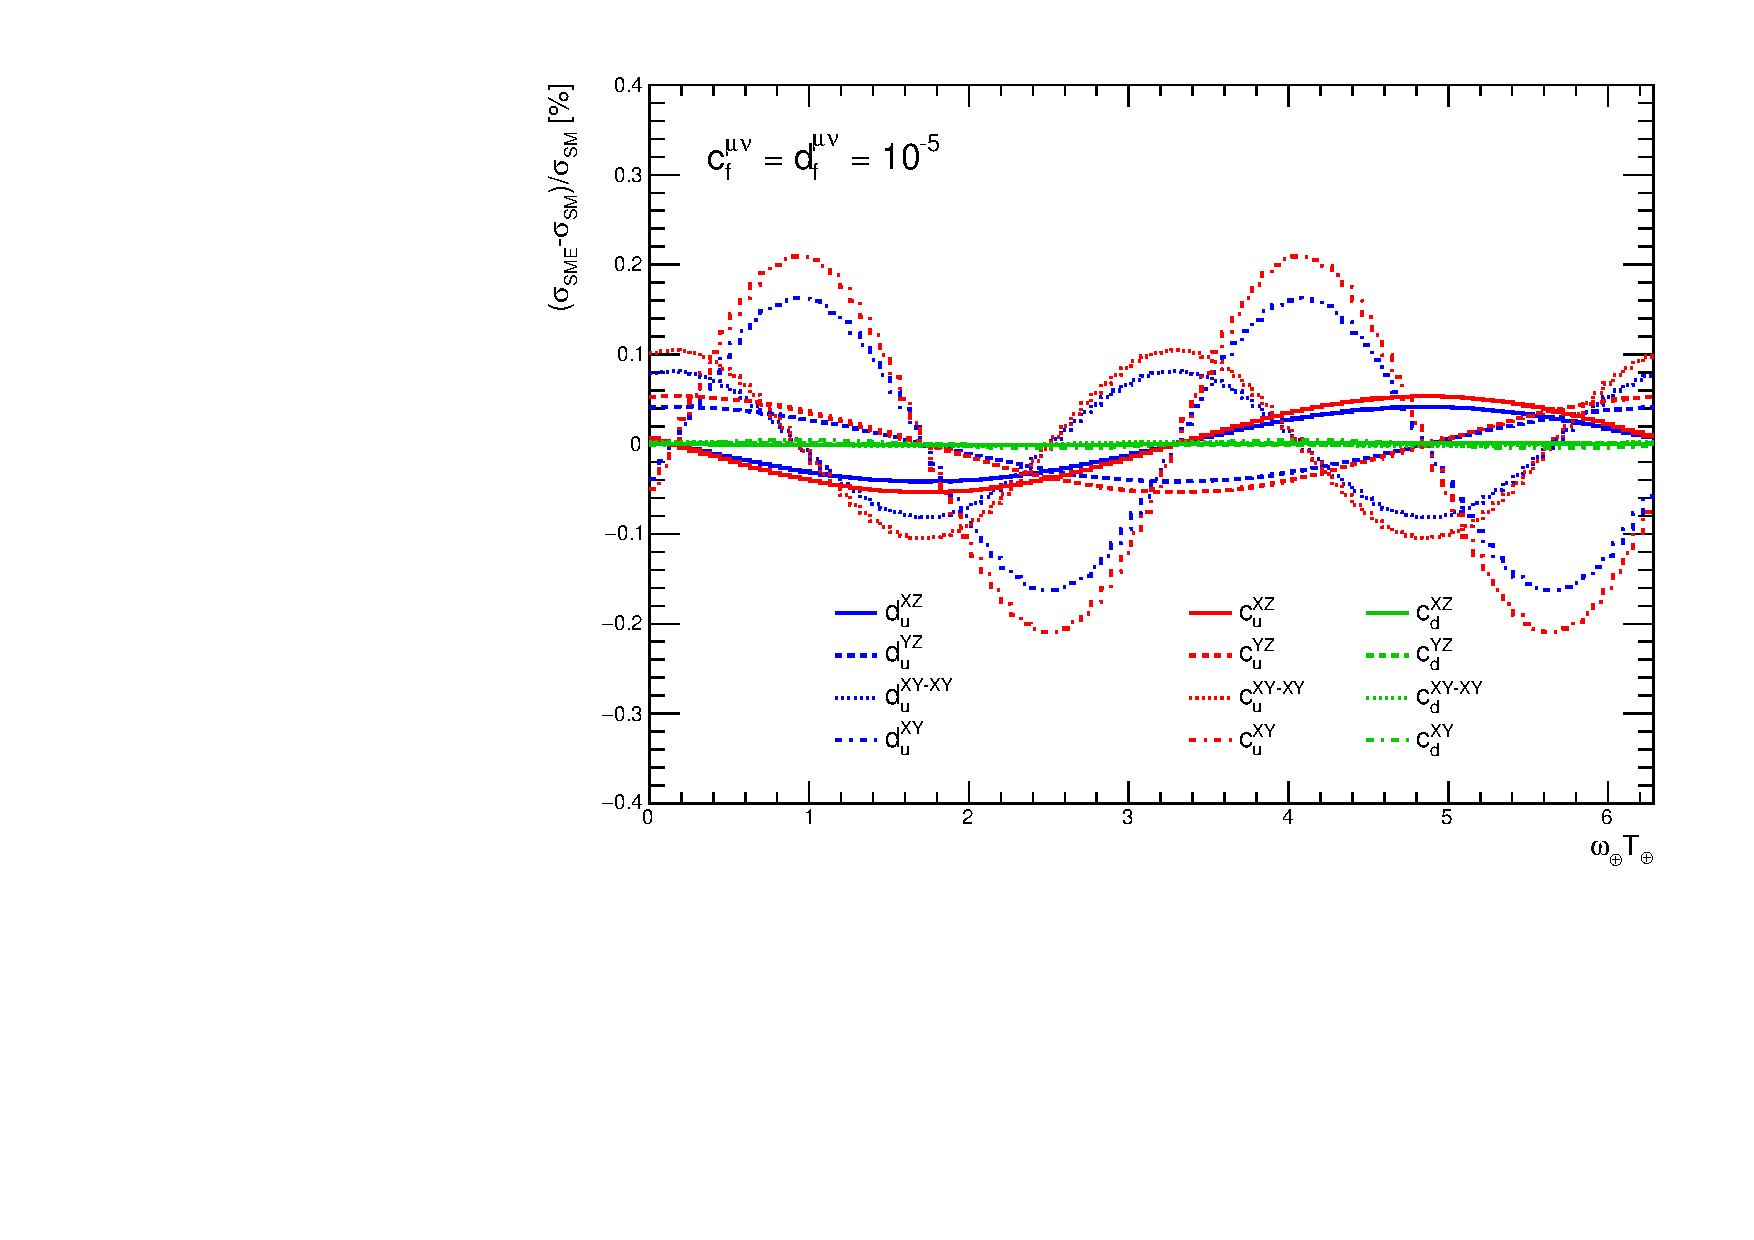
\includegraphics[scale=0.75]{figs/SMEeffects.pdf}
	\caption{Functional forms of the time dependence associated with 
    each SME coefficient, as expressed in 
    Eqs.~\ref{eq:duXZ}-\ref{eq:cdXY}.}
	\label{fig:SME_effects}
\end{figure}
%
%
\subsection{Nonminimal quark-sector effects}
%
%
Thus far we have focused on the minimal SME in the quark sector.
From an effective field theory viewpoint, nonrenormalizable operators 
of mass dimension $d>4$ parametrize the effects of new physics 
suppressed by the associated characteristic energy scale. The more
energetic a given process the more relevant nonrenormalizable operators
become. For example, a $d=5$ operator has a SME coefficient
with dimension GeV$^{-1}$. The dominant (tree-level) insertions of
this operator introduces an expansion parameter $\delta = (E/\Lambda)$,
where $E$ is the process scale (e.g. the energy
of the initial-state partons in the Drell-Yan procees), 
and $\Lambda$ the scale of new physics (e.g the Planck scale). 
The larger $E$ is, the more relevant the expansion parameter. A $d=6$
operator would include a leading-order correction controlled
by $\delta^2$. Though clearly suppressed relative to the
$d=5$ operator, since $\Lambda$ is fixed the influence of the $d=6$
operator grows more rapidly. Nonrenormalizable operators
are extensively studied in Lorentz-invariant new-physics
searches at the LHC because they generically
parametrize new physics too heavy to be 
produced on-shell by the colliding beamlines. 

Nonrenormalizable effects from the nonminimal SME 
have also been investigated in 
Drell-Yan dilepton production~\cite{Kostelecky:2019fse}. 
The $d=5$ Lagrange density was considered:
%
\begin{equation}
{\cal L}_{a^{(5)}} = -\frac{1}{2}\sum_f a_f^{(5)\mu\alpha\beta}
\bar\psi_f \gamma_\mu iD_{(\alpha}iD_{\beta)}\psi_f + \text{h.c.},
\end{equation}
where the parenthesis surrounding $\alpha, \beta$ denotes index symmetrization
and h.c. is shorthand for Hermitian conjugation. 
%
\begin{table}[t]
\centering
\begin{tabular}{|c|c|c|}\hline
& {\textbf{HERA}} & {\textbf{LHC}} \\ \hline
 $|a^{(5)TXX}_{\text{S}u}- a^{(5)TYY}_{\text{S}u} |$& $4.3\times 10^{-7}$ & $1.5\times 10^{-8}$ \\
 $|a^{(5)TXY}_{\text{S}u}|$& $6.5\times 10^{-7}$ & $2.7\times 10^{-9}$ \\
 $|a^{(5)TXZ}_{\text{S}u}|$ & $1.1\times 10^{-6}$ & $7.2\times 10^{-9}$ \\
 $|a^{(5)TYZ}_{\text{S}u} |$&  $7.4\times 10^{-7}$ & $7.0\times 10^{-9}$ \\
\hline
\end{tabular}
\caption{Comparison of HERA and LHC sensitivity to $a^{(5)}$-type coefficients.
The limits from HERA come from a recent ZEUS analysis~\cite{ZEUS:2022msi} and coincide with the
positive upper limit report in units of GeV$^{-1}$. 
The quoted values for LHC come from simulations assuming uncorrelated
systematic uncertainties. Table adapted from Refs.~\cite{Kostelecky:2019fse},\cite{ZEUS:2022msi}.
\label{tablea5}}
\end{table}
%
We will refer to the SME coefficients that 
appear as the $a^{(5)}$-type coefficients. From Table~\ref{tablea5} 
it is observed that the LHC could expect up to two orders 
of magnitude more sensitivity to these coefficients than what was obtained
by the ZEUS Collaboration~\cite{ZEUS:2022msi}. This increased sensitivity
has its origin in the increased collision energy of the LHC relative to HERA.

The predictions of Table~\ref{tablea5} are limited to photon exchange. When
electroweak bosons are exchanged, the $a^{(5)}$-type coefficients cannot be treated in isolation.
The reasons are exactly the same as for why the $c$-type coefficients
can not be treated independently of the $d$-type coefficients when
a $W^\pm$ or $Z$ is exchanged, as discussed in Sec.~\ref{ssec:LIVDY}. 
Analogous to the $d$-type coefficients, the other set of coefficients
relevant for the nonminimal effects probed here are called the $b^{(5)}$-type 
coefficients. 

Predictions for Drell-Yan on the $Z$ pole and including the
$b^{(5)}$-type coefficients are currently being calculated by
the theory STA members~\cite{LS24}. Because the $a^{(5)}$-
and $b^{(5)}$-type coefficients are analogous in structure to the
$c$- and $d$-type coefficients, we expect a similar enhancement
of nonminimal LIV signatures on the $Z$ pole. Therefore, it is reasonable
to expect a greater relative sensitivity to these coefficients
than estimated in Table~\ref{tablea5}. 

Since the $a^{(5)}$- and $b^{(5)}$-type coefficients have an odd number
of Lorentz indices, they also produce striking CPT-violating effects.
For example, in deep inelastic scattering, when summing
the antiquark contributions these coefficients appear with opposite
signs to the quark contributions. Thus, for the sea quarks in the proton
the effect cancels out. The ZEUS analysis was therefore only sensitive
to the $u$ and $d$ quark $a^{(5)}$ coefficients. In contrast,
the leading Drell-Yan diagram involves $q\bar q$ fusion. The appearance
of particle and antiparticle in this diagram does not
produce the same cancellation effect as in deep inelastic scattering. 
Therefore, the Drell-Yan process can probe the CPT properties
of quarks. Our analysis will be the first probe of the CPT 
properties of sea quarks.





\clearpage
\section{Methodology} %% [Uta]
\label{lab:Methodology}
\el{Definition of the observable, i.e. binned cross section. Comment on uncertainties on efficiencies and on origin of the Monte Carlo correction. Stress that using efficiencies from data removes time dependent effects. Explain the $F_\text{MC}(\mu)$ has two uncertainties: a statistical one and a systematic one ($\delta \mu \sim 1$). The latter is due to the uncertainty on the SM cross section used as normalization and is constant across the three main periods of data taking (2015+2016, 2017, 2018).}
%%%% 
%%% upto here, motivation, SME frame, how to compute sidereal effects are done.
%%% Keep this section simple. No need to describe details on Z counting. 
%%% Let's explain contents / input from Z counting. 
%%% Is the luminosity measurement published? 
%%%




\subsection{Use of the Z-counting luminosity measurement}

The results to be used for this analysis are those presented in the Z-counting luminosity measurement~\cite{ATL-DAPR-PUB-2021-001}\footnote{The results originally reported were based on the full Run-2 results obtained using the Tag10 ATLAS official luminosity measurement. The search presented in this Note will use the updated results using the luminosity Tag11.}. This Section contains a brief introduction to the methodology used for a time-dependent measurement of the Z-boson production at ATLAS as presented in the Z-counting PUB note. \color{red}{Appendix~\ref{sec:Zcount_app}}\color{black} contains a full overview of the methodology, transferred to a more commonly used ATLAS analysis framework.\\

The methodology was first established as an alternative measurement of the luminosity recorded by the ATLAS experiment, where the Z-boson decay into dileptons during \color{red}{physics running}\color{black} is used to provide additional checks against residual time, pile-up, or beam-condition-dependent biases that may affect the baseline ATLAS luminosity values, the determination of which is detailed in Ref~\cite{ATLAS-CONF-2019-021}.

The Drell-Yan production of dilepton pairs is a well understood process, with the clean Z-boson signature of two high-transverse momentum, oppositely charged leptons\footnote{Z-boson decays to $\tau$ leptons or quarks are not considered here, as they are much more difficult to reconstruct and prone to very high background levels.} providing robustness against varying pileup conditions. Thus, a luminosity measurement can be obtained by measuring the number of produced Z-bosons, $N_Z$, using the formula

\begin{equation}
\int \mathcal{L}_Z dt = \frac{N_Z^{corr}}{\sigma_Z}
\label{eq:Zcount:RawLumi}
\end{equation}

where $\sigma_Z$ is the Z production cross section. Experimentally, precise measurements of $\sigma_{Z\rightarrow e^+e^-}$ ($\sigma_{Z\rightarrow \mu^+\mu^-}$) have been obtained with systematic uncertainties (excluding luminosity) of about 1.0\% (1.5\%)~\cite{ATLAS:2019zci}. The value of the $Z\rightarrow \ell^+\ell^-$ cross-section is predicted by calculations at next-to-next-to-leading order QCD with a total uncertainty of 3-4\% at 90\% CL, where the uncertainty is driven by the current knowledge of the proton parton distribution functions (PDFs). As the uncertainties in the baseline ATLAS luminosity are below 2\%~\cite{ATLAS-CONF-2019-021}, the Z-counting luminosity is not competitive as an absolute measurement, but has many powerful features as a relative luminometer.

The Z-counting procedure is performed as a function of time, in units of "luminosity blocks" (LBs), the smallest time interval for which luminosities are measured in ATLAS. These typically correspond to 60 seconds intervals, but occasionally account for a shorter amount of time depending on trigger or data acquisition configurations.

For each lepton flavour the raw rate of detected $Z$s is measured on a LB-by-LB basis. To obtain the $Z$ production rate, the raw rate is corrected to account for the trigger and reconstruction efficiencies. These data-driven efficiencies are subject to additional corrections, derived as a function of the average number of simultaneous collisions, $\left< \mu \right>$, from Monte Carlo simulations. A small background subtraction is also applied in order to account for dilepton pairs in the event selection phase space originating from diboson and $t\bar{t}$ events.

%% Thus, the general form for calculating the $Z$-counting based instantaneous luminosity as shown in Eq~\ref{eq:Zcount:RawLumi} has to be modified as follows
%% 
%% \begin{equation}
%% \mathcal{L}_{Z\rightarrow \ell^+\ell^-} (LB) = \frac{N_{Z\rightarrow \ell^+\ell^-}(LB)\cdot (1-f_\text{bkg})}{\sigma_\text{theo}\times A^\text{MC}_{Z\rightarrow \ell^+\ell^-}\cdot \varepsilon^\text{T\&P}_{Z\rightarrow \ell^+\ell^-}(LB) \cdot F^\text{MC}_{Z\rightarrow \ell^+\ell^-}(\left< \mu \right>)\cdot t(LB)}
%% \label{eq:Zcount:ZLumi}
%% \end{equation}
%% 
%% where

$N_Z^{corr}$ is obtained after correcting following effects which described in the public note\cite{ATL-DAPR-PUB-2021-001}:

\begin{itemize}
   \item The fraction of background in the Z peak region, which is 0.5\% in both the electron and muon channel.
   \item $Z\rightarrow \ell^+\ell^-$ cross-section of 1970$~pb$. 
   \item Acceptance of the fiducial phase space. 
   \item Trigger efficiency and reconstruction efficiency measured for each LB.
   \item Efficiency correction factor to take into account the average pileup, $<\mu>$, dependence. 
   \item duration of each LB.
\end{itemize}

Each correction is carefully assessed in a per-LB (or per-pileup) basis, obtaining an independent measurement of the instantaneous luminosity recorded by ATLAS, with which we can monitor the time and pileup stability of the nominal luminosity measurement or, in the case of this analysis, search for Lorentz-invariance violation in the production of the Z-boson cross-section.\\

The methodology was originally developed to run on the DataQuality ATLAS analysis framework, using the WZFinder tool. This framework, with which the results this analysis will be based on were obtained, runs on Tier-0 ATLAS data.

\subsection{Sidereal phase in this analysis}
%The final distribution to probe the LIV effect is the double ratio, $R_D$ defined in Eq.~\ref{eq:double_ratio}, 

In the actual analysis, we use a double ratio between the $N_Z^{corr}$ and the integrated luminosity ($\mathcal{L}i$). 
% The $N_Z^{corr}$ is from the reconstructed $Z$ bosons ($N_Z^i$).
\begin{equation}
  R_D = \frac{ N_{Z_i}^{corr} /\Sigma N_{Z_i}^{corr}}{\int\mathcal{L}_i dt / \Sigma \int\mathcal{L}_idt},
\label{eq:double_ratio}
\end{equation}
where the index $i$ indicates bin number as function of the sidereal phase. 
By normalizing with total summation of each value, systematic uncertainties related to normalization are fully canceled, 
also most of uncertainties on object efficiencies and all theory related uncertainties are canceled. 
However, any time-dependent effects may remain and need to be evaluated, e.g. arising from the 
time-dependence of the baseline ATLAS luminosity measurement. These effects are discussed in Section~\ref{lab:Systematic}.

Some details for these input variables described below.

\begin{itemize}
 \item \textbf{Integrated luminosity for each LB, $\int\mathcal{L}_idt$}, provided by the ATLAS luminosity group.
   The measured luminosity of Lucid is used in the analysis. 
   Need to have selection and merging scheme for ``bad'' LBs and LBs which have shorter duration. 
   As a cross check, the measured luminosity based on the track counting method is used.
 \item \textbf{the corrected number of $Z$ bosons}, $N_{Z_i}^{corr}$, for each LB of $i$.
   The luminosity group provides three values with error for each LB, the electron channel, the muon channel and the combined value.
   We study each channel. The final result will be extracted with the combined value.
   The error of each measurements includes statistical uncertainty and the systematic uncertainty of the corrections. 
  \item \textbf{Sidereal bin assignment}, described in Eq.\ref{eq:sid_phase_bin} in Section~\ref{sec:phase_comp}. 
   The start and end time stamps of each LB is available in the unix time. 
   We use them and compute a time stamp of middle of each lumi block, and convert it in the sidereial time at ATLAS detector in sun centered frame.
   The number of bin can be optimized according to data statistics. We set default number of bins as 100 according to a Toy study described in Section~\ref{sec:number_of_bins}.
\end{itemize}



%%%%%
Summary table of the input LBs for each year is shown in Table~\ref{tab:data_LBs}.
Here, need to describe selection of LBs. Remove low duration, zero for one of output, etc.. 
%%%%%

\begin{table}
\centering 
\begin{tabular}{c | c c c} % centered columns (4 columns)
year & number of runs & number of LBs & Integrated luminosity ($fb^{-1}$)\\
\hline
2015  & ~66  & ~22,850  & ~3.10  \\
2016  & 150  & ~91,111  & 33.28  \\
2017  & 186  & ~86,471  & 44.61  \\
2018  & 194  & ~92,711  & 58.70  \\
\hline 
Total & 596  & 293,143  & 139.69 \\
\end{tabular}
\caption{\label{tab:data_LBs} Summary of input data for each year}
\end{table}

Once the binned histogram on the double ratio is obtained, we fit it with expected formula discussed in Section~\ref{sec:theorydetails}.
Also, we are planning to fit with genelic functional form. 


\subsection{Samples and steps to unblind the LIV search}

 This analysis is the first search in ATLAS to probe the sidereal effect, we do not look final result until ATLAS exotic group approve the unblinding. 
The blind the result is established by NOT perform the final fit with probing period with sidereal period (23 hour 56 minutes 04 seconds) with real data.
This is checked by TOY study described in Section~\ref{lab:ToyStudy}. We found that looking at data with 24 hours to verify day-night effect would unblind the data effectively. 

Because any physics process could have LIV effect, we would not rely on any specific kinetics region as a ``control region''.
Instead, we check the data behavior with different periods to compute the phase.
We have verified that if we use 1 hour as a period to compute the phase, instead of the sidereal
period $T_{\text{sid.}}$, any LIV signal can be wiped out.
With this approach, we can verify the final statistical analysis procedure and statistical uncertainty.
However, it turned out that 1 hour period is too short to reveal the potential issue,
i.e. missing measurements on particular time period (any experimental effect or analysis issue could be wiped out as well).
Therefore, we propose following steps to unblind:

\begin{enumerate}
\item check any bias with data driven TOY sample (randomly generated number of Z with data luminosity measurement)
\item analyze the real data set with scrambling time stamp
\item probe $R_D$ with probing period of 1 hour
\item probe $R_D$ with probing period with 7 hours and 24 hours step by step.
\end{enumerate}
After confirming no bias within statistics and systematics uncertainties, unblind the $R_D$ with the sidereal phase.

Step-1 and -2 are described in Section~\ref{lab:ToyStudy} and \ref{lab:DataScrambling}. 
Exotic group already approved to proceed Step-2 in a LPX meeting in September 2023.
Once all statistics tool and systematic studies are done, we would ask to move Step-3 and later. 

At the end, we do not use normal ATLAS MC simulation samples. 
This is because nominal systematic effects from both theoritical and experimental sources are canceled out in the double ratio. 
Only time dependent systematics are affected in the search. This is discussed in Section~\ref{lab:Systematic}.

%%More description on blinding strategy are discussed in Section.~\ref{sec:step_by_step_unblind_test}.

\subsection{Statistics analysis on the fitting as function of the sidereal phase}
%%The framework of the fit is Roofit. Details, i.e. treatment of systematic uncertainties, are described in Section~\ref{lab:Syst_stat}.

A statistics treament to extract the LIV search result is summarized here. 
Basically we do a binned fit as function of the probing phase with chisquare minimization. 
In this fit, we include extra terms to take into account systematic uncertainty. 

%% \subsection{Statistical analyses}
\label{lab:DataScrambling_stat}

%% chi2 analysis.

The chi-squared ($\chi^{2}$) fit method is used to determine a signal strengh from a givent
 dataset (a double ratio). This method is commonly employed in various scientific 
 disciplines to assess how well a model describes the observed data.
 The formula for the chi-squared statistic is:
 \begin{equation}
    \chi^2 = \sum \frac{(O_i - E_i)^2}{\sigma_i^2},
 \end{equation}

 where 
 \begin{itemize}
    \item $i$ is the bin index, and it's range is [0-99] becuase we use 100 bins.
    \item $O_i$ is the observed value for data point $i$.
    \item $E_i$ is the expected value for data point $i$.
    \item $\sigma_i^2$ is the uncertainty (standard deviation) associated with the observed value.
 \end{itemize}

Datasets and theory models:
\begin{itemize}
    \item Dataset is a  double ratio obserable binned in a probing perioud.
     Total number of bin is 100 (see Section.~\ref{lab:ToyStudy}). The dataset is eigher toy, scrambled data or real data when
     this analysis is unblinded.
    
     \item Thery models are analytic fuctions predicted by SME theory described in 
     Section~\ref{lab:Theory}. Each model is fitted to a dataset independent to other models.
     and Each model has a free parameter, $\mu$, which is the signal strength.
    
    \item Degree of freedom: 100 bins minus number of free parameters which one in our case.
     So the DoF is 99.
\end{itemize}
 %% Ablet

\subsubsection{$\chi^{2}$ fit}
For a given theory prediction $f$ with a parameter $\mu$ and dataset $\{y_{i}\}$, a $\chi^{2}$ estimator is constructed as:
\begin{equation}
    \chi^{2} (\mu) = \sum_{i}^{100} \left(\frac{y_{i} - f_{i}(\mu)}{\sigma_{i}}\right)^{2}.
\end{equation}\label{eq:chi2_estimator}

Here, the $\{\sigma_{i}\}$ are the uncertainties carried with the dataset (e.g statistical uncertainties of the dataset). In this analysis, the double ratio observable, $R$, contains 100 data points within the 0 to $2\pi$ range (sidereal phase). Therefore, the index $i$ runs from 1 to 100. 

\subsubsection{Profiled $\chi^{2}$ fit}
The $\chi^{2}$ estimator described in the EQ~\ref{eq:chi2_estimator} does not consider a systematic effect. Thus, this section introduces a $\chi2^{2}$ estimator with an additional nuisance parameter.

Assume this analysis has a systematic uncertainty $\textbf{S}$.  A sigma variation of this systematic will the shifts (absolute shifts with sign) a data point by $s_{i}$ in $ith$ bin; the data point $y_{i}$ increase or decrease by $s_{i}$. In this case, the dataset and theory predictions are $\{y_{i}\}$, $f_{i}(\mu)$, and input uncertainties are $\{\sigma_{i}\}$ and $\{s_{i}\}$.

The formula \ref{eq:chi2_estimator} does not take into account the $s_{i}$. We can add one nuisance parameter, $\beta$, to the theoretical model to carry a systematic variation. The modified theory will be:
\begin{equation}
    F_{i}(\beta, \mu) = f_{i}(\mu) + \beta s_{i}.
\end{equation}\label{eq:modefied_func}
Here, $\{s_{i}\}$ are constant (they have plus and minus sign). The $\beta$ is a standard normal Gaussian distributed variable centered at ZERO and varies within [-1,1] range, which corresponds to a plus-minus one sigma variation of the systematic $\textbf{S}$. In this case, the original $\chi^{2}$ estimator become a two-parameter estimator (profiled $\chi^{2}$ estimator):

\begin{equation}
    \chi^{2} (\beta, \mu) = \sum_{i}^{100} \left(\frac{y_{i} - F_{i}(\beta, \mu)}{\sigma_{i}}\right)^{2} + \beta^{2}.
\end{equation}\label{eq:profile_chi2_estimator}


\subsubsection{Test with toy systematics}

%The toy dataset used in this study is provided by Yuji. 
The toy data represents the signal-free data corresponding to full ATLAS Run2 luminosity. Plots in Figure~\ref{fig:data_with_sys_shift} show the Double Ratio (R) of this signal-free dataset. The black color shows the nominal data points, and the gray color shows the shifted data due to a systematic variation (e.g., plus one sigma). The blue line in the right plot is a signal shape and strength used to obtain a shift in data. 

\begin{figure}
\centering
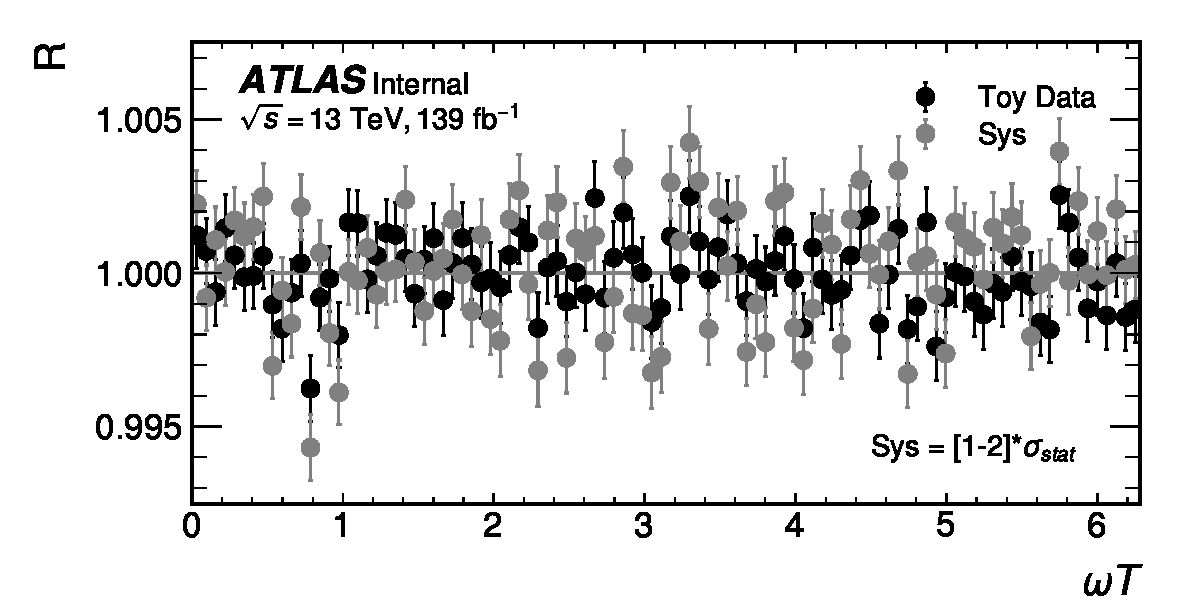
\includegraphics[width=0.45\textwidth]{figs/App_profile_chi2/profile_chi2_rnd_sys_PlusOneSigma_shifts}
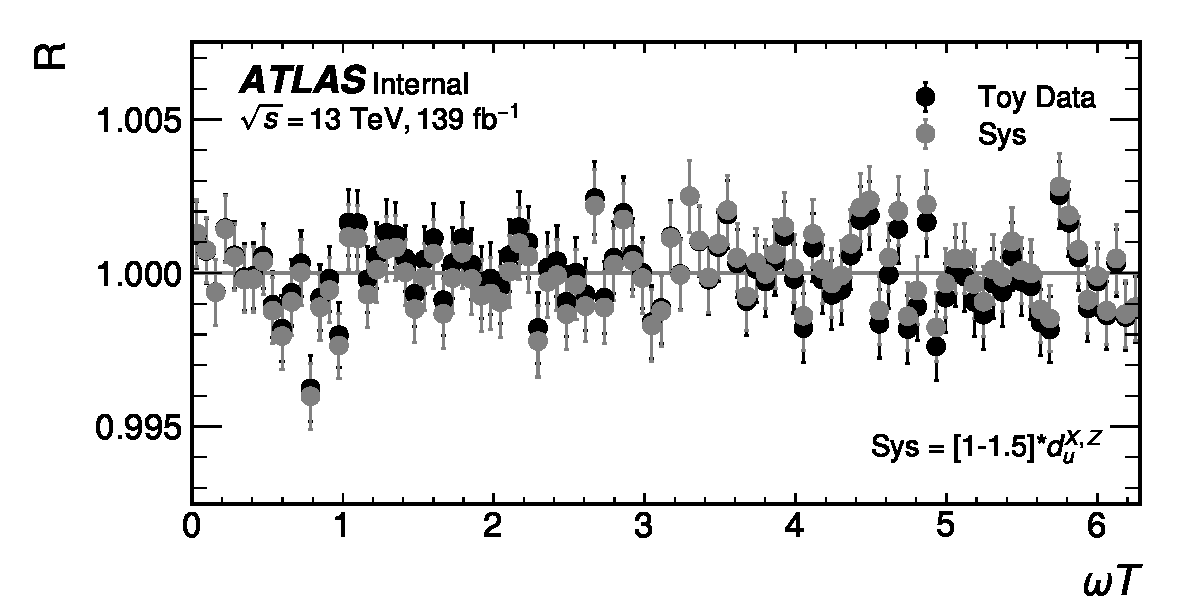
\includegraphics[width=0.45\textwidth]{figs/App_profile_chi2/profile_chi2_shape_sys_du_XZ_shifts}
\caption{The black color shows nominal data points, and the gray color shows shifted data points due to a systematic variation. The randomized systematic impacts top left (case 2). The systematic effect introduces a shape to data, top right (case 3)}
\label{fig:data_with_sys_shift}
\end{figure}



To test the profiled $\chi^{2}$ estimator, three cases for a set of systematic uncertainty are considered:

\begin{enumerate}
    \item $\beta = 0$. This is a default case where no systematic variations are included. This is for $\chi^{2}$ fit to the data points with black color in Figure~\ref{fig:data_with_sys_shift}, without profiling.
    
    \item $s_{i} = RandomChoise([-1,1])\times RandomNumber([1,2])\times \sigma_{i}$. Both the sign and size of $s_{i}$ are randomly chosen. Because we assume that the systematic impacts on data points are not correlated. 
    
    \item $s_{i} = RandomNumber([1,1.5])\times {d_{u}^{X,Z}}_{i}$. Add small signals to mimic shifts in data due to systematics. The size of $s_{i}$ is randomized between 1-1.5 times the signal in $ith$ point.
\end{enumerate}

Case 1 is one parameter $\chi^{2}$ fit since $\beta = 0$. To perform the profiled $\chi^{2}$ fit, $scipy$ python package is used (it is easier to implement in Python rather than in RooFit). The original $\chi^{2}$ fit in equation \ref{eq:chi2_estimator} is used to validate $scipy$ and $RooFit$ packages. Results from these two packages agreed very well up to high precision. 

In case 2, the size and sign of $s_{i}$ are randomly chosen so that they don't introduce some shapes (for example, cos- or sin-like oscillation). The $s_{i}$ are the difference between black and gray points in the left plot in Figure~\ref{fig:data_with_sys_shift}.

In case 3, the size and direction of shifts (sign) $\{s_{i}\}$ are introduced by a signal shape. The $d_{u}^{X,Z}$ is considered the shape, and the signal strength is set to $\mu = 1E^{-5}$. The $\{s_{i}\}$ are the difference between black and gray points in the right plot in Figure~\ref{fig:data_with_sys_shift}. As we can see in the plot, the shifts in data will introduce a signal-like shape to the dataset.


\begin{figure}
\centering
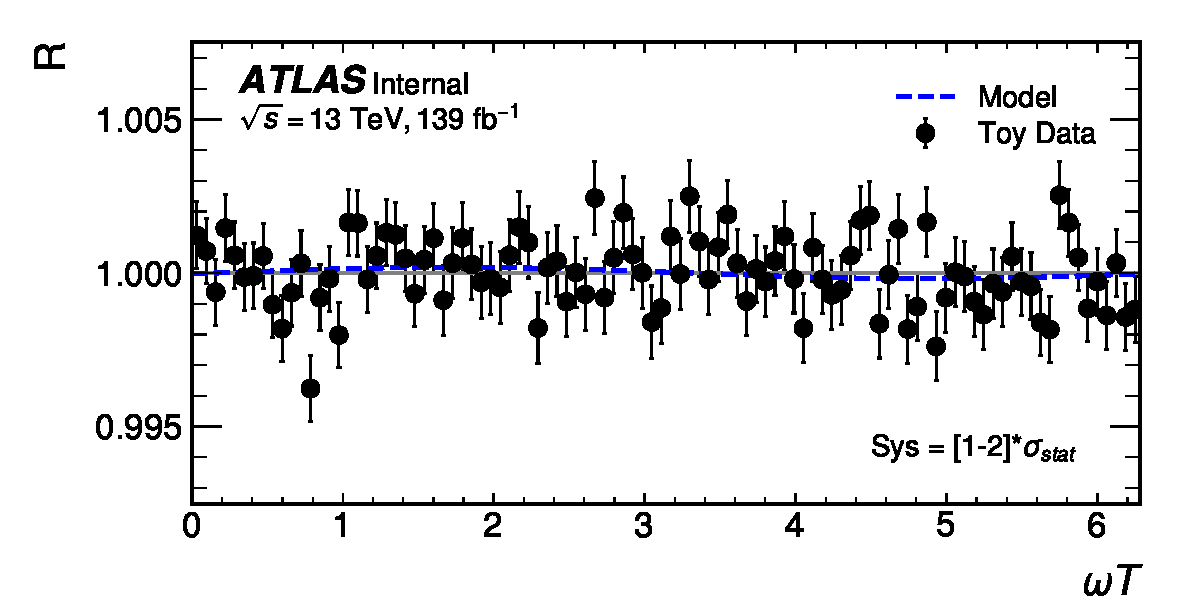
\includegraphics[width=0.45\textwidth]{figs/App_profile_chi2/profile_chi2_rnd_sys_PlusOneSigma_ToyData_postfit}
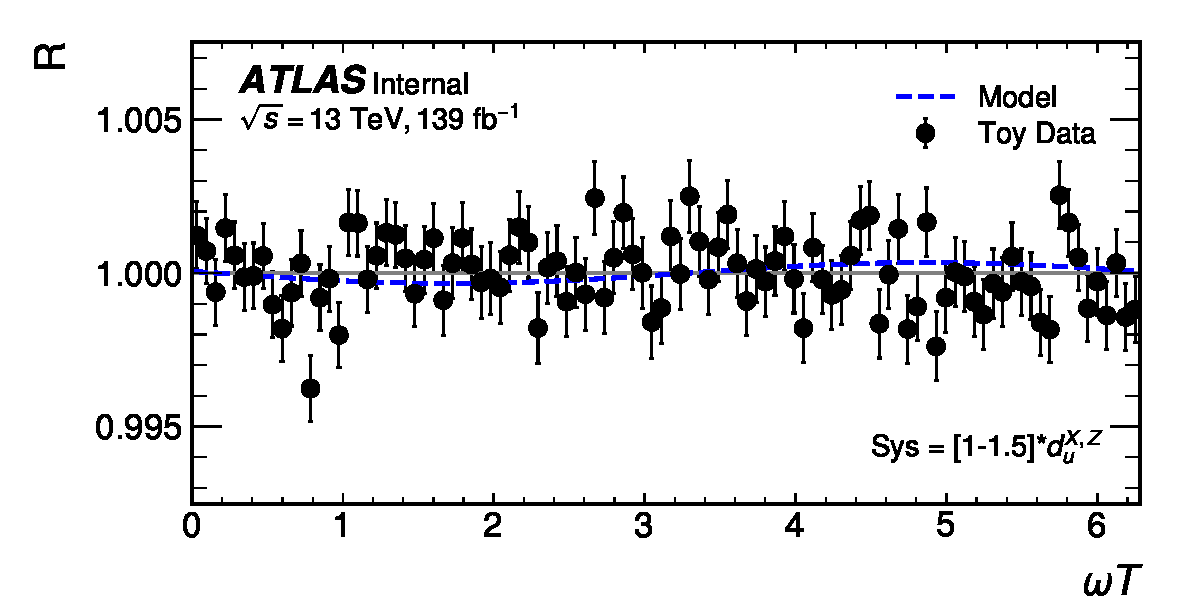
\includegraphics[width=0.45\textwidth]{figs/App_profile_chi2/profile_chi2_shape_sys_du_XZ_postfit}\\
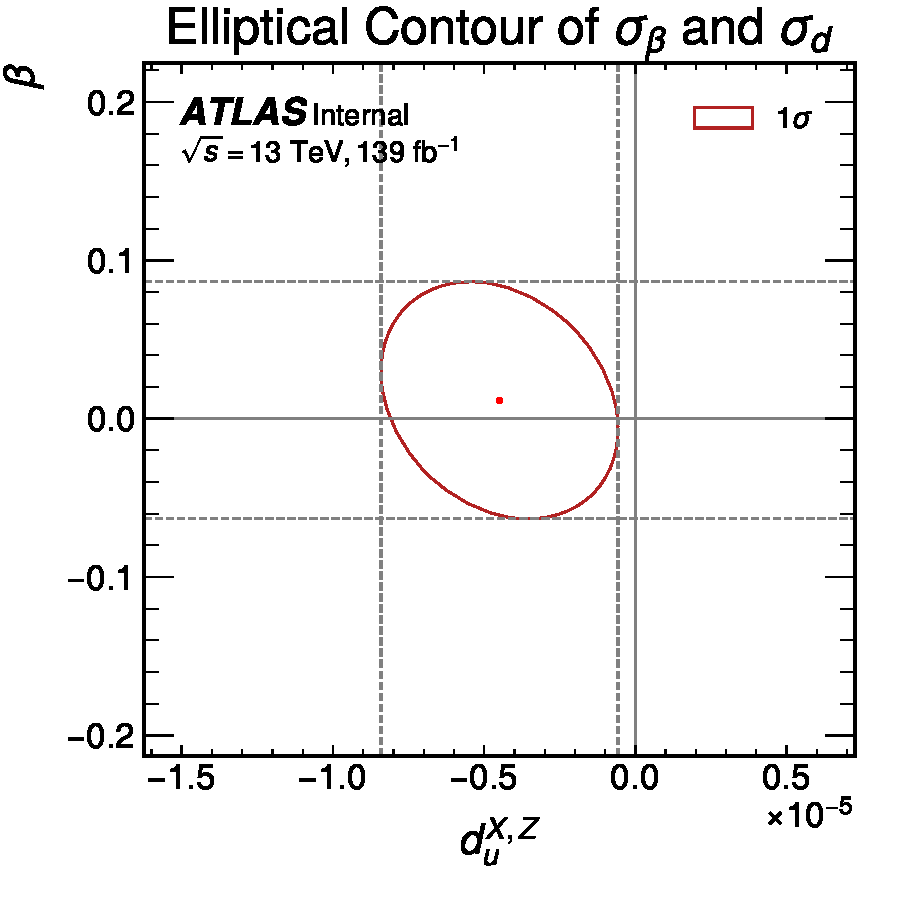
\includegraphics[width=0.45\textwidth]{figs/App_profile_chi2/profile_chi2_rnd_sys_du_XZ}
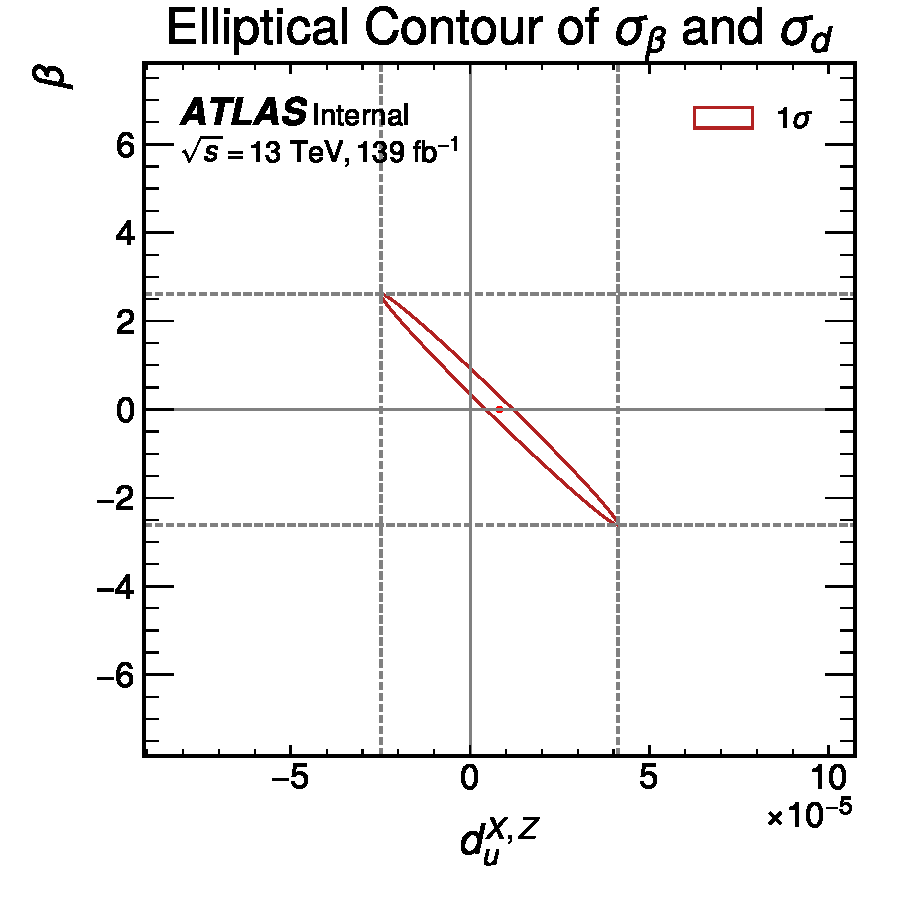
\includegraphics[width=0.45\textwidth]{figs/App_profile_chi2/profile_chi2_shape_sys_du_XZ}
\caption{Fit from the randomized systematic impacts top left (case 2). The fit with the systematics introduces a shape to data, top right (case 3). Corresponding one sigma contours from profiled $\chi^{2}(\beta, \mu)$ in the bottom plots.}
\label{fig:profile_chi2_fit_test}
\end{figure}

A profiled $\chi^{2}$ (Equition~\ref{eq:profile_chi2_estimator}) is fitted to Cases 2 and 3. The fit results are shown in Figure~\ref{fig:profile_chi2_fit_test}. The top left plot shows the toy data and fitted model (blue line). Since data is signal free and the systematic impact does not introduce any shapes to data, the fitted signal amplitude (or strength) is small. The bottom left plot shows the corresponding one-sigma contour. The input size for $\beta$ is [-1, 1] and it is constrained after the fit. The top right plot Figure~\ref{fig:profile_chi2_fit_test} shows the toy data and fitted model with profiled shape systematics (this systematic introduces signal like shape). From the corresponding contour plot (bottom right), one can see the impact of systematic uncertainty on the parameter estimation.

Fitted signal strength and its uncertainty from three cases are compared in Figure~\ref{fig:profile_chi2_fit_comparison}. The impact of the systematic is small for randomized uncertainty (Sys(rnd)) because this kind of systematics does not introduce oscillation shapes. The large impact is seen for a systematic that can introduce a signal-like shape (Sys(CORR)) to data.


\begin{figure}
\centering
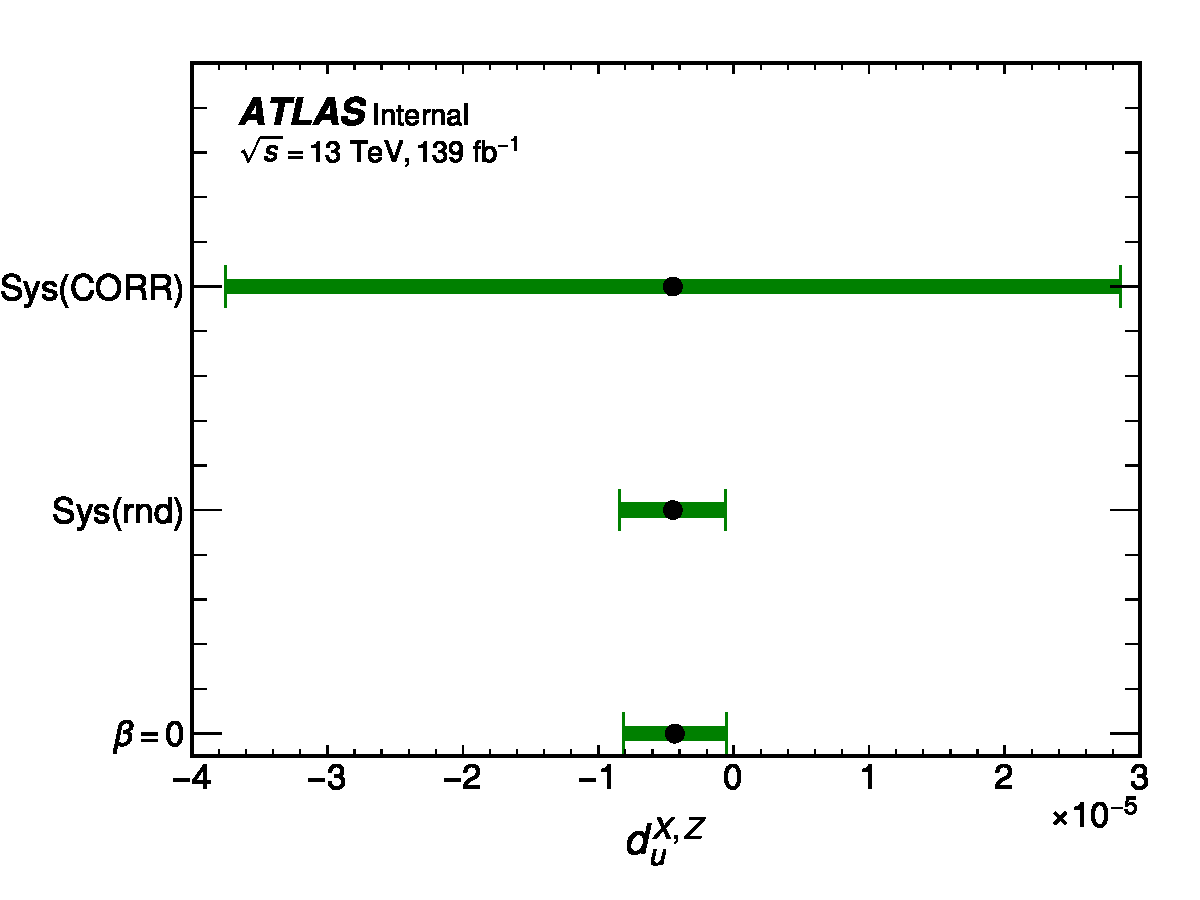
\includegraphics[width=0.6\textwidth]{figs/App_profile_chi2/profile_chi2_compare_fit_results}
\caption{Comparison of the fitted parameter $d_{u}^{X,Z}$ from $\chi^{2}$ ($\beta=0$) and profiled $\chi^{2}(\beta, \mu)$ fits using toy systematics in Case 2 (Sys(rnd)) and 3 (Sys(CORR)).}
\label{fig:profile_chi2_fit_comparison}
\end{figure}
 %% Ablet




\clearpage
\section{Time dependence of data}  
\label{sec:data_time_dependence}
We begin our study by discussing the large time dependence observed in data and associated to the actual interval of time over which the LHC delivered luminosity to the ATLAS detector. 

Data is taken in small chunks, called LumiBlocks (LBs), with an average duration of about 60 sec. The distribution of LB durations across the entire Run~II data taking period (2015-2018) is shown in the left panel of figure~\ref{fig:LBs}. The total number of LBs during Run-II is summarized in Table~\ref{tab:LBs}.

\begin{figure}[H]
\centering
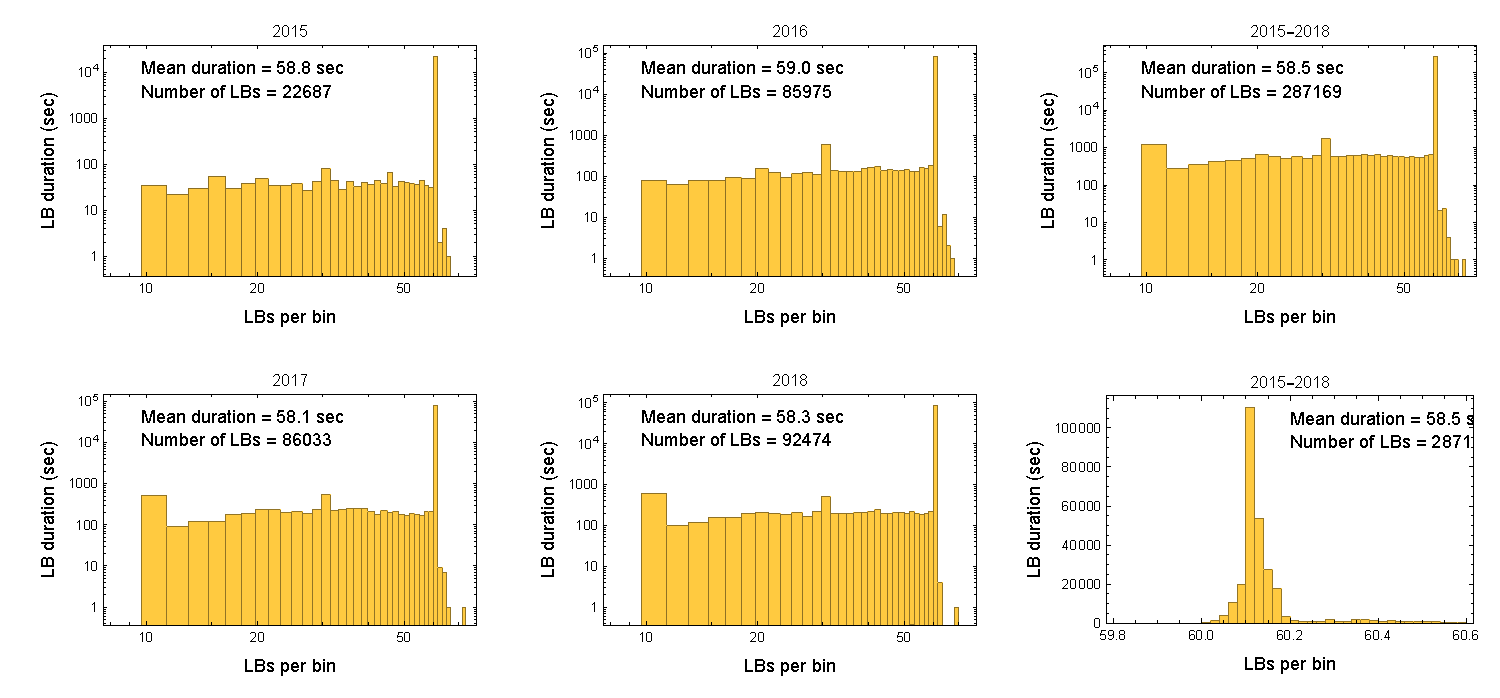
\includegraphics[width=\textwidth]{figs/Mathematica-oldchi2/LB_duration_log_allyears}
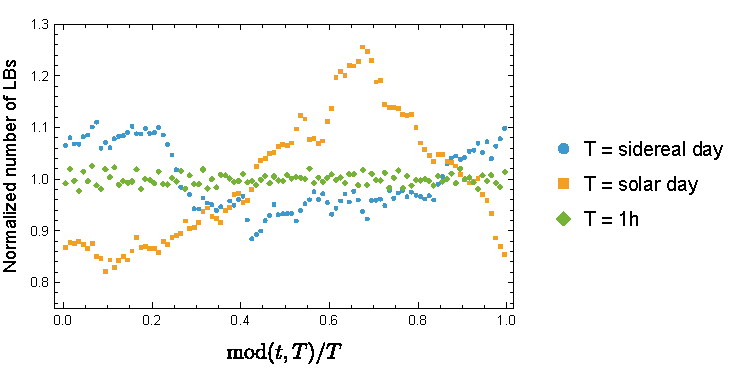
\includegraphics[width=0.7 \textwidth]{figs/Mathematica-oldchi2/LB_phase}
\caption{Distribution of the LumiBlocks durations (top panel) and phases (bottom panel) across the entire data taking period.}
\label{fig:LBs}
\end{figure}

\begin{table}[H]
    \centering
    \begin{tabular}{|c|c|} \hline
         Year & Number of LBs \\ \hline 
         2015 & 22687 \\
         2016 & 85975 \\
         2017 & 86033 \\
         2018 & 92474 \\ \hline
         total & 287169 \\ \hline
        \end{tabular}
    \caption{Yearly and total number of LBs in Run-II.}
    \label{tab:LBs}
\end{table}

Each LB has a unique time stamp which is taken to be the average of its initial and final time stamps. From this time stamp, the time in the Sun-Centered-Frame is constructed as discussed in Sec.~\ref{sec:timeshift}. Finally, for a giving testing period (e.g. solar day ($T = 24\text{hr}$), sidereal day ($T = 23.93\text{hr}$), \ldots), each time stamp, $t$, is converted to a phase in the interval $[0,1]$:
%
\begin{align}
t \rightarrow \phi (T) = \text{mod}[ t , T ]/T  \; .  
\end{align}
%
In the right panel of figure~\ref{fig:LBs} we show the normalized distribution of the LBs phases calculated using three testing periods: $T_\text{solar}$, $T_\text{sidereal}$ and $T = 1 \text{hr}$. As can be seen there is a very large solar day dependence, with much more data taken near $\phi (T_\text{solar}) \sim 0.7$ which corresponds to the middle of the night in Geneva (about $4\text{am}$).  

In figure~\ref{fig:Lumi_phase} we show the normalized distribution of the integrated Luminosity across the four data taking years. The pattern of peak luminosity recorded in the middle of the night is consistent across the four years. The 2015-2018 cumulative distribution is essentially identical to the LB distribution presented in figure~\ref{fig:LBs}.

\begin{figure}[H]
\centering
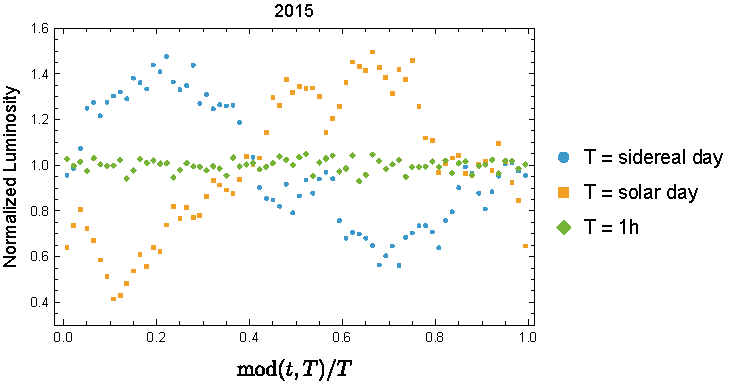
\includegraphics[width=0.49\textwidth]{figs/Mathematica-oldchi2/Lumi_phase_2015}
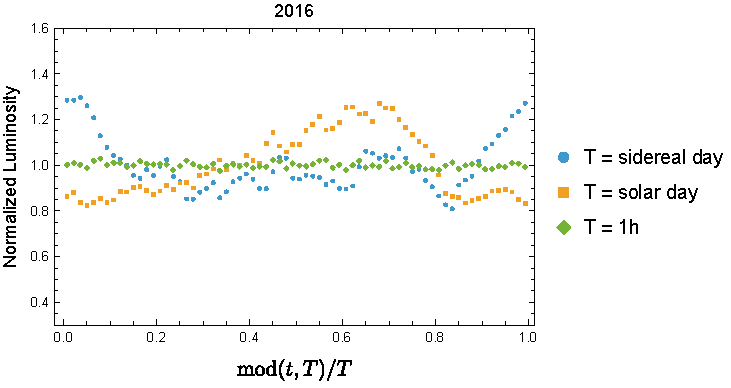
\includegraphics[width=0.49\textwidth]{figs/Mathematica-oldchi2/Lumi_phase_2016}
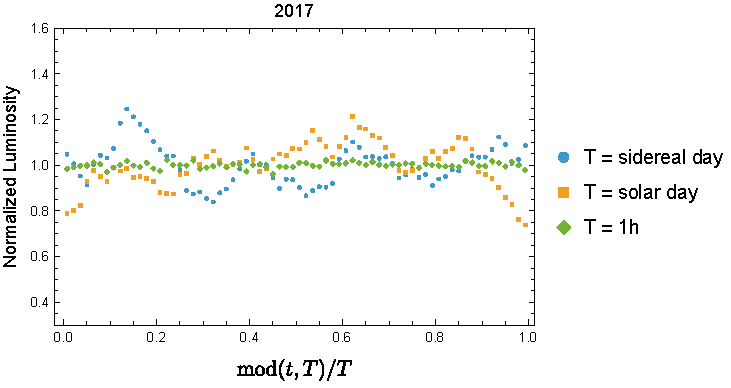
\includegraphics[width=0.49\textwidth]{figs/Mathematica-oldchi2/Lumi_phase_2017}
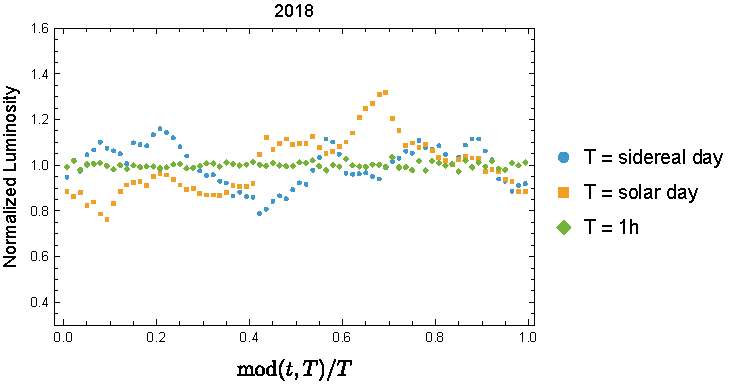
\includegraphics[width=0.49\textwidth]{figs/Mathematica-oldchi2/Lumi_phase_2018}
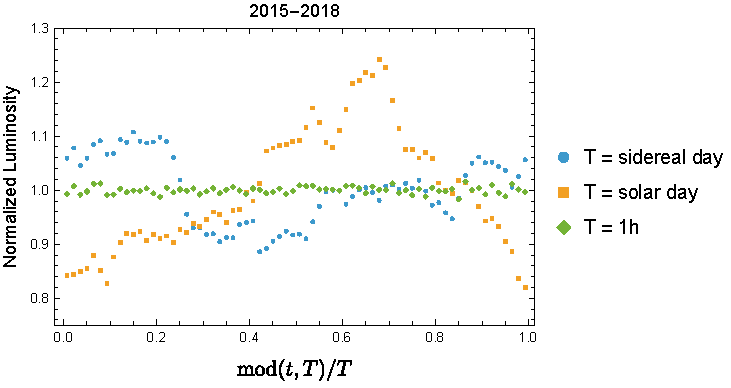
\includegraphics[width=0.49\textwidth]{figs/Mathematica-oldchi2/Lumi_phase_allyears}
\caption{Normalized distribution of the integrated Luminosity as a function of the phase for the four data taking years.}
\label{fig:Lumi_phase}
\end{figure}

In the next step, we construct time distributions of simulated $Z$ counts. For each LB, we combine time stamp, efficiency ($\varepsilon$), Monte Carlo correction factor ($F_\text{MC}(\mu)$ with $\mu$ taken from data) and luminosity with the fiducial NNLO SM cross section:
%
\begin{align}
N_\text{fid}^\text{SM} (t) = \sigma_\text{SM}\cdot  A_\text{SM}\cdot \varepsilon(t) \cdot  F_\text{MC} (\mu(t)) \cdot {\cal L}_\text{inst}(t) \cdot \Delta t
\label{eq:NZsim}
\end{align}
%
where all time dependent quantities are taken from data. The resulting normalized distribution as a function of phase is shown in the left panel of figure~\ref{fig:NZsimulated}. We also Poisson sampled each $N_\text{fid}^\text{SM} (t)$ and constructed the corresponding normalized distribution, which is presented in the right panel of figure~\ref{fig:NZsimulated}.

\begin{figure}[H]
\centering
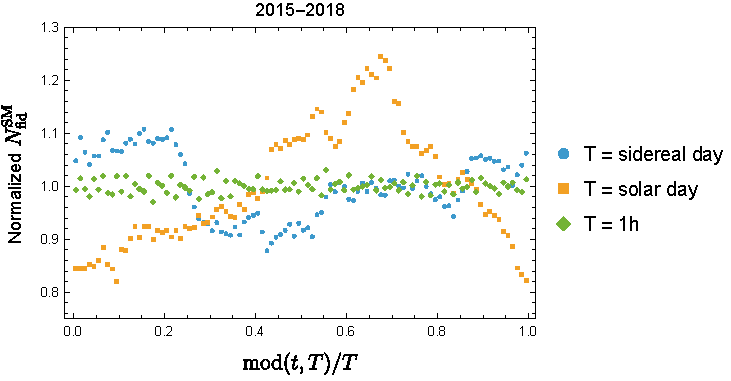
\includegraphics[width=0.49\textwidth]{figs/Mathematica-oldchi2/Nfiducial_theory_phase}
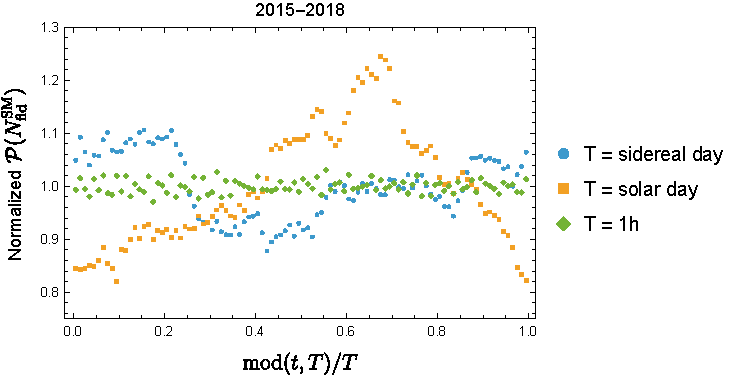
\includegraphics[width=0.49\textwidth]{figs/Mathematica-oldchi2/Nfiducial_theory(Poisson)_phase}
\caption{Normalized distribution of simulated $Z$ counts. Time stamps, Luminosity and efficiencies are taken from data. The left panel is obtained from the central values of the simulated Z counts in each LB ($N_\text{fid}^\text{SM}$). The right panel is obtained by Poisson sampling Z counts in each LB (${\cal P} (N_\text{fid}^\text{SM})$).}
\label{fig:NZsimulated}
\end{figure}

From this preliminary distributions it is clear that the data has a strong time dependence which is completely dominated by the actual data taking pattern. In the next section we begin exploring the time distribution of the cross section measured in each LB which is expected to be free from these effect. 
%

\clearpage
\section{Double ratio simulation studies: single sampling}
\label{sec:double_ratio}
In this section we begin our investigation of the ratio $R_D$. All the studies we present use use the full information for each LB with the exception of the actual $Z\to (e^+e^-,\mu^+\mu^-)$ counts. The basic strategy, which we implement in small sequential steps, is to use the SM fiducial cross section $\sigma_\text{fid}$ and the measured efficiencies and luminosities, to simulate $Z$ counts in each LB. This part of the analysis is, therefore, completely blinded to Drell-Yan data. We take 
$\sigma_\text{fid} = \sigma_\text{SM}^\text{NNLO} A^\text{MC}_{Z\to \ell^+\ell^-}$, where the NNLO cross section is $\sigma_\text{SM}^\text{NNLO} = 1929\; \text{pb}$ and the Monte Carlo calculated acceptances for electrons and muons are $A^\text{MC}_{Z\to e+e^-} = 0.2996$ and $A^\text{MC}_{Z\to \mu^+\mu^-} = 0.3323224$, respectively.

We label each subsection using the formula used to calculate the corrected $Z$ count. We focus on the muon case only.

\subsection{\texorpdfstring{$N_Z^\text{corr} = \sigma_\text{fid} \cdot {\cal L}_\text{inst}\cdot  \Delta t$}{NZcorr = sigmafid * Linst * Delta t}}
\label{ssec:all_constant}
We begin by a toy study in which we fix the SM fiducial cross section to $\sigma_\text{fid} = 750\; \text{pb}$ and the instantaneous luminosity to ${\cal L}_\text{inst} = 10^{34}\; \text{cm}^{-2} \text{s}^{-1} = 10^{-2}\;  \text{pb}^{-1} \text{s}^{-1}$. The duration $\Delta t$ of each LB is taken from data. The $Z$ count in each LB (identified by its time stamp $t$) is then constructed as\footnote{$N_Z^\text{corr}$ is the $Z$ count corrected for effects of efficiencies. In this toy study we do not include efficiencies but keep the notation for consistency.} $N_Z^\text{corr}(t) = {\cal P} (\sigma_\text{fid} \cdot {\cal L}_\text{inst} \cdot \Delta t)$, where $\Delta t$ is the duration of the LB at time $t$ and ${\cal P}$ stands for Poisson sampling. We then choosing a testing period $T$ (sidereal day, solar day, 1 hour) and histogram the $N_Z^\text{corr}(t)$ counts and the luminosities ${\cal L}= {\cal L}_\text{inst} \cdot \Delta t$ in 100 bins of $\text{mod} (t,T)/T \in [0,1]$. The resulting counts are $N_{Z_i}^\text{corr}$ and ${\cal L}_i$ with $i\in[1,100]$. We then construct the ratio 
%
\begin{align}
R_D = \frac{ N_{Z_i}^\text{corr} / \sum N_{Z_i}^\text{corr} }{ {\cal L}_i / \sum {\cal L}_i} \; .
\label{eq:RD}
\end{align}
%
We calculate this ratio separately for data taken in 2015+2016, 2017 and 2018. The three distributions are then stitched together in the range $[0,3]$ as shown in figure~\ref{fig:toy_RD}. We see that the standard deviation of the 100 bins for this example is $\sigma_{R_D} = 1.5 \times 10^{-3}$.

Using the signal formulas discussed in Eqs.~\ref{eq:duXZ}-\ref{eq:cdXY}, we perform a fit to the 12 SME coefficients. The results are shown in figure~\ref{fig:toy_fits}. The central values are not zero because they have been obtained by a single Poisson sampling.

Finally, we perform a Gaussianity check on the distribution of a given sidereal bin (we choose bin 1) by resampling 1000 times. The histogram of $R_D$ in the first bin and various Gaussianity tests are presented in figure~\ref{fig:toy_Gaussianity}.

\begin{figure}[H]
\centering
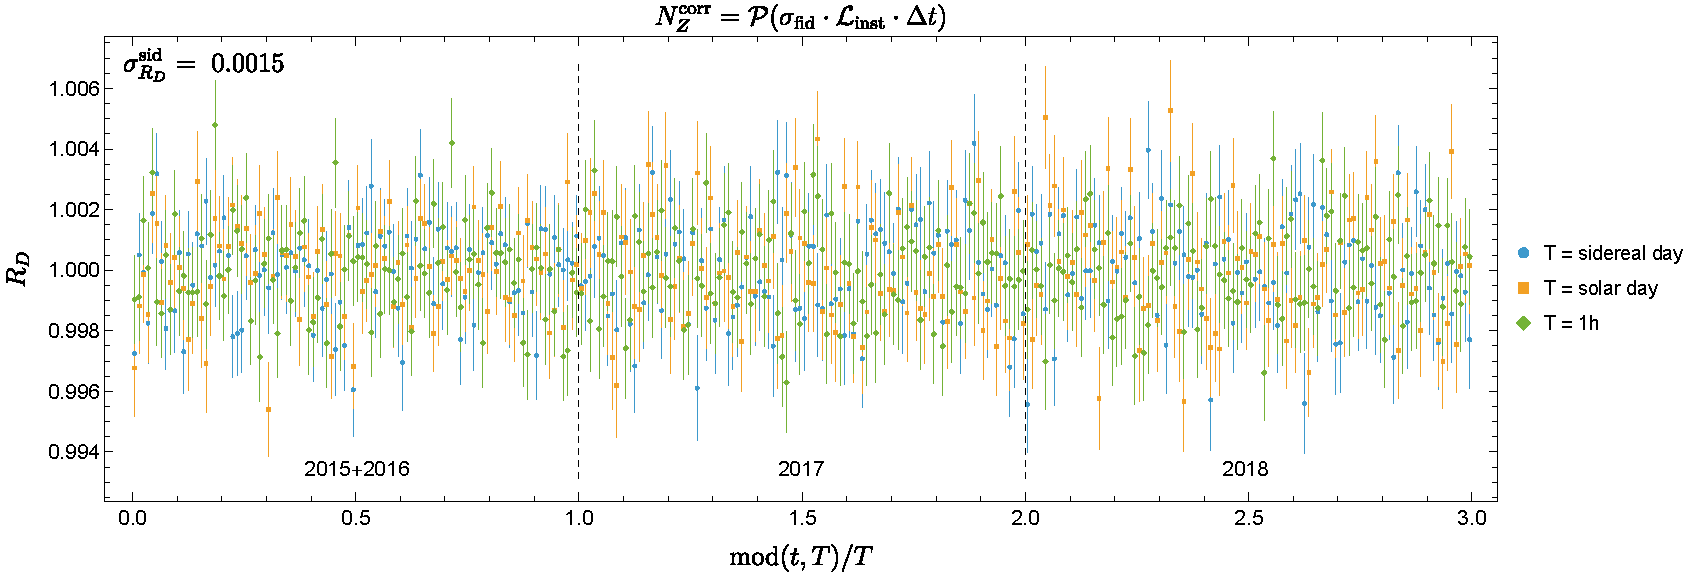
\includegraphics[width=\textwidth]{figs/Mathematica-oldchi2/xs(sigmaFID)_phase(LBlive)}
\caption{$R_D$ distribution for the toy study described in the text. In the upper right corner we show the standard deviation of the sidereal day distribution.}
\label{fig:toy_RD}
\end{figure}

\begin{figure}[H]
\centering
\begin{minipage}[H]{0.49\textwidth}
    \vspace{1.6cm}
    \centering
    \begin{tabular}{|l|c|}
        \hline
        $d_u^{XZ}$ & $(-1.4 \pm 3.0)\times 10^{-6}$ \\
        $d_u^{YZ}$ & $(-1.9 \pm 2.8)\times 10^{-6}$ \\
        $d_u^{XX-YY}$ & $(0.24 \pm 1.6)\times 10^{-6}$ \\
        $d_u^{XY}$ & $(3. \pm 7.7)\times 10^{-7}$ \\
        $c_u^{XZ}$ & $(-1.1 \pm 2.4)\times 10^{-6}$ \\
        $c_u^{YZ}$ & $(-1.5 \pm 2.2)\times 10^{-6}$ \\
        $c_u^{XX-YY}$ & $(0.19 \pm 1.2)\times 10^{-6}$ \\
        $c_u^{XY}$ & $(2. \pm 6.0)\times 10^{-7}$ \\
        $c_d^{XZ}$ & $(-0.48 \pm 1.1)\times 10^{-4}$ \\
        $c_d^{YZ}$ & $(-0.66 \pm 0.98)\times 10^{-4}$ \\
        $c_d^{XX-YY}$ & $(0.8 \pm 5.4)\times 10^{-5}$ \\
        $c_d^{XY}$ & $(1.1 \pm 2.7)\times 10^{-5}$ \\
        \hline
        \end{tabular}
\end{minipage}
\begin{minipage}[H]{0.49\textwidth}
    \vspace{0pt}
    \centering
   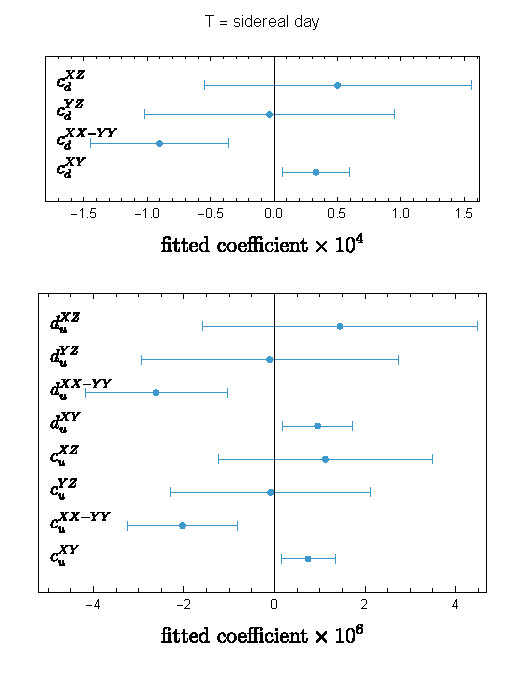
\includegraphics[width=\textwidth]{figs/Mathematica-oldchi2/xs(sigmaFID)_phase(LBlive)_fit}
\end{minipage}
\caption{Fit results for the $N_Z = \sigma_\text{fid} \cdot {\cal L}_\text{inst} \cdot \Delta t$ study.}
\label{fig:toy_fits}
\end{figure}

\begin{figure}[H]
\centering
\begin{minipage}[H]{0.49\textwidth}
    \vspace{0.8cm}
    \centering
   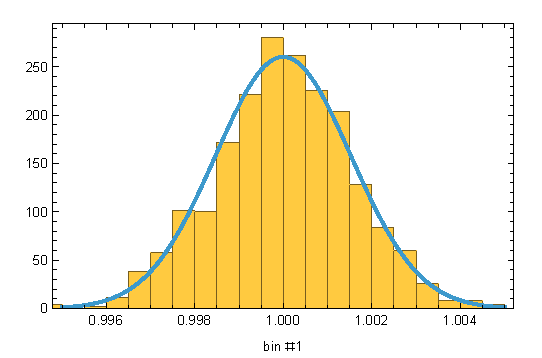
\includegraphics[width=\textwidth]{figs/Mathematica-oldchi2/xs(sigmaFID)_phase(LBlive)_bin1_GaussianityHist}
\end{minipage}
\begin{minipage}[H]{0.49\textwidth}
    \vspace{0cm}
    \centering
    \begin{tabular}{l|ll}
        & \text{Statistic} & \text{P-Value} \\ \hline 
 \text{Anderson-Darling} & 0.418497 & 0.830165 \\
 \text{Baringhaus-Henze} & 0.672449 & 0.459449 \\
 \text{Cram{\' e}r-von Mises} & 0.06435 & 0.786632 \\
 \text{Jarque-Bera ALM} & 0.570246 & 0.748594 \\
 \text{Kolmogorov-Smirnov} & 0.0200947 & 0.806376 \\
 \text{Kuiper} & 0.0353756 & 0.594088 \\
 \text{Mardia Combined} & 0.570246 & 0.748594 \\
 \text{Mardia Kurtosis} & 0.343257 & 0.731405 \\
 \text{Mardia Skewness} & 0.419634 & 0.51712 \\
 \text{Pearson }$\chi ^2$ & 31.424 & 0.445 \\
 \text{Shapiro-Wilk} & 0.99867 & 0.668533 \\
 \text{Watson }$U^2$ & 0.061504 & 0.578408 \\
        \hline
        \hline
        \end{tabular}
\end{minipage}
\caption{Gaussianity checks of the distribution of $R_D$ in the first sidereal bin.}
\label{fig:toy_Gaussianity}
\end{figure}

\subsection{\texorpdfstring{
$N_Z^\text{corr} = \sigma_\text{fid} \cdot \epsilon \cdot F_\text{MC}(\mu)\cdot {\cal L}$ 
with $\delta \epsilon= \delta F^\text{MC}(\mu) = 0$}{NZcorr = sigmafid * epsilon * FMC * L with delta epsilon = delta FMC = 0}}
\label{ssec:no_eFMC_errors}
%
In the next study we include the effects of the efficiency ($\epsilon$) and of the Monte Carlo correction ($F_\text{MC}(\mu)$) to produce a more accurate simulation of the actual $Z$ count. At this stage we take the values of $\epsilon$ and $\mu$ in each LB from data but do not include uncertainties on either $\epsilon$ nor $F^\text{MC}(\mu)$. The dependence of $F^\text{MC}(\mu)$ on $\mu$ is~\cite{ATL-DAPR-PUB-2021-001}:
%
\begin{align}
F^\text{MC}_{Z\to e^+e^-} & = 
\begin{cases}
    0.907628 - 0.000328652\; \mu - 3.0512 \times 10^{-6} \mu^2 & 2015/2016 \\
    0.904096 - 0.000172139\; \mu - 4.35328\times 10^{-6} \mu^2 & 2017 \\
    0.90238 - 8.75767 \times 10^{-5} \mu - 5.79201 \times 10^{-6} \mu^2 & 2018 \\
\end{cases},
\\
F^\text{MC}_{Z\to \mu^+\mu^-} & = 
\begin{cases}
    0.990074 - 5.34716 \times 10^{-6} \mu - 3.23366 \times 10^{-6} \mu^2 & 2015/2016 \\
   0.991619 - 1.21674\times 10^{-4} \mu - 1.58362 \times 10^{-6} \mu^2 & 2017 \\
    0.990808 - 9.99749*10^{-5} \mu - 1.40241 \times 10^{-6} \mu^2 & 2018 \\
\end{cases}.
\end{align}

We construct the simulated $Z\to\mu\mu$ counts for each LB using $N_Z(t) =  {\cal P} ( \sigma_\text{fid} \cdot \epsilon \cdot F^\text{MC}(\mu) \cdot {\cal L})$ and the corresponding corrected count $N_Z^\text{corr} = N_Z(t)/(\epsilon \cdot F^\text{MC}(\mu))$. 

The double ratio $R_D$ is the constructed as in Eq.~(\ref{eq:RD}). The resulting distribution is shown in figure~\ref{fig:RD_noerrors}. The standard deviation of the 100 bins for this example is $\sigma_{R_D} = 1.9 \times 10^{-3}$. Using the signal formulas discussed in Eqs.~\ref{eq:duXZ}-\ref{eq:cdXY}, we perform a fit to the 12 SME coefficients. The results are shown in figure~\ref{fig:RD_noerrors_fits}. The central values are not zero because they have been obtained by a single Poisson sampling.

\begin{figure}[H]
\centering
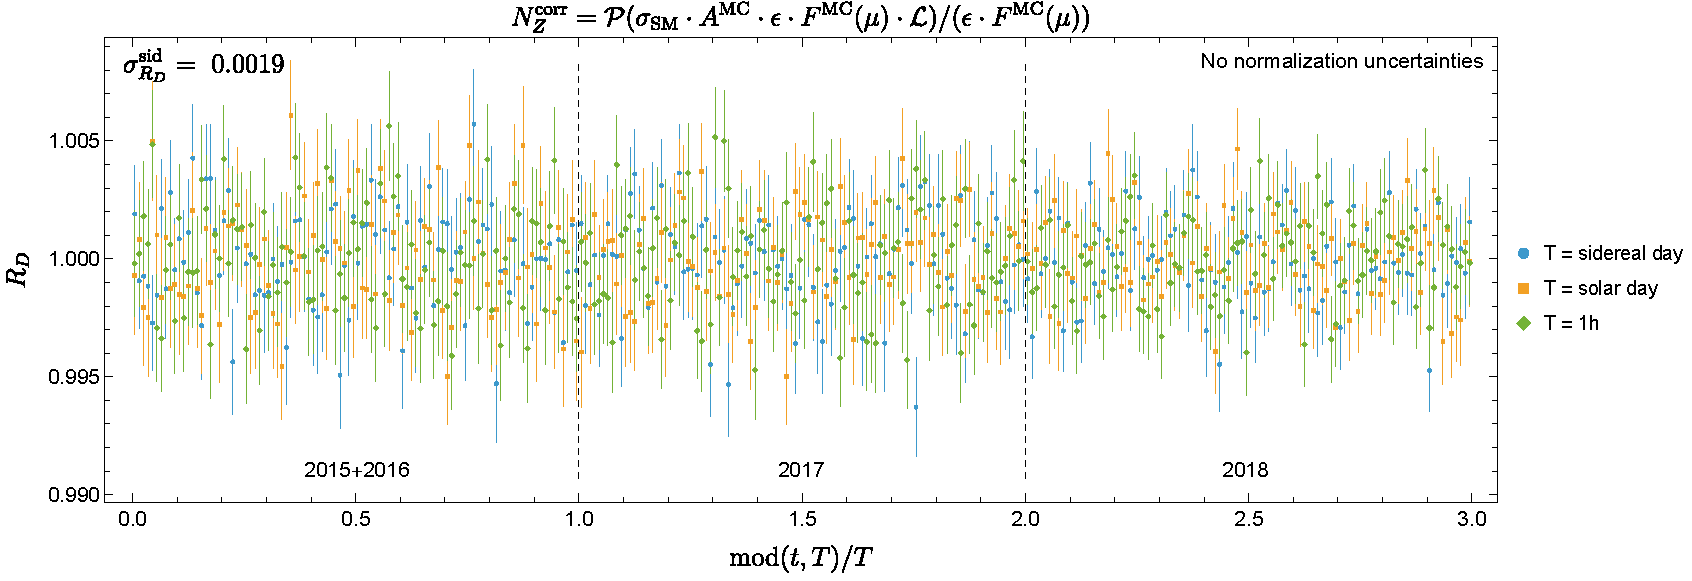
\includegraphics[width=\textwidth]{figs/Mathematica-oldchi2/xs(sigmaFID eps FMC)_noGauss_noNormErr_phase}
\caption{$R_D$ distribution for the toy study described in the text. In the upper right corner we show the standard deviation of the sidereal day distribution.}
\label{fig:RD_noerrors}
\end{figure}

\begin{figure}[H]
\centering
\begin{minipage}[H]{0.49\textwidth}
    \vspace{1.6cm}
    \centering
    \begin{tabular}{|l|c|}
        \hline
        $d_u^{XZ}$ & $(-1.0 \pm 4.0)\times 10^{-6}$ \\
        $d_u^{YZ}$ & $(1.1 \pm 3.8)\times 10^{-6}$ \\
        $d_u^{XX-YY}$ & $(-1.9 \pm 2.0)\times 10^{-6}$ \\
        $d_u^{XY}$ & $(12.7 \pm 9.5)\times 10^{-7}$ \\
        $c_u^{XZ}$ & $(-0.8 \pm 3.1)\times 10^{-6}$ \\
        $c_u^{YZ}$ & $(0.9 \pm 3.0)\times 10^{-6}$ \\
        $c_u^{XX-YY}$ & $(-1.5 \pm 1.5)\times 10^{-6}$ \\
        $c_u^{XY}$ & $(9.8 \pm 7.4)\times 10^{-7}$ \\
        $c_d^{XZ}$ & $(-0.4 \pm 1.4)\times 10^{-4}$ \\
        $c_d^{YZ}$ & $(0.4 \pm 1.3)\times 10^{-4}$ \\
        $c_d^{XX-YY}$ & $(-6.7 \pm 6.8)\times 10^{-5}$ \\
        $c_d^{XY}$ & $(4.4 \pm 3.3)\times 10^{-5}$ \\
        \hline
        \end{tabular}
\end{minipage}
\begin{minipage}[H]{0.49\textwidth}
    \vspace{0pt}
    \centering
   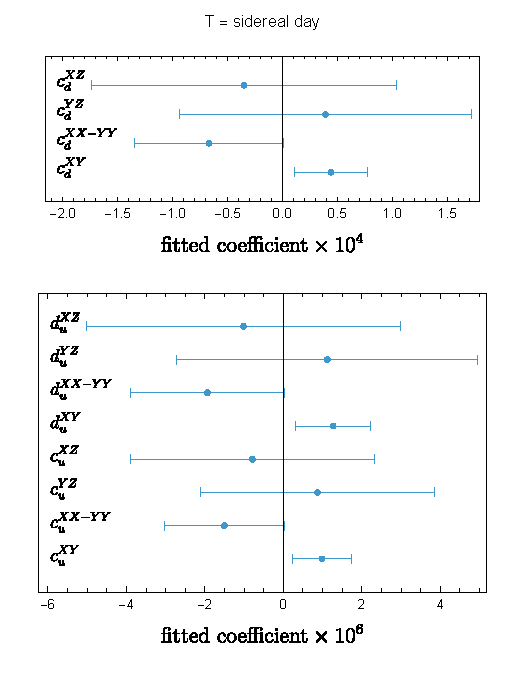
\includegraphics[width=\textwidth]{figs/Mathematica-oldchi2/xs(sigmaFID eps FMC)_noGauss_noNormErr_fit}
\end{minipage}
\caption{Fit results for the $N_Z = \sigma_\text{SM}\cdot A^\text{SM} \cdot \epsilon \cdot F^\text{MC}(\mu) \cdot {\cal L}$. No uncertainties on $\epsilon$ and $F^\text{MC}(\mu)$ are included.}
\label{fig:RD_noerrors_fits}
\end{figure}


\subsection{\texorpdfstring{
$N_Z^\text{corr} = \sigma_\text{fid} \cdot \epsilon \cdot F_\text{MC}(\mu)\cdot {\cal L}$ 
with $\delta \epsilon \neq 0$ and $\delta F^\text{MC}(\mu) = 0$}{NZcorr = sigmafid * epsilon * FMC * L with delta epsilon != 0 and delta FMC = 0}}
\label{ssec:no_FMC_errors}
%
We now repeat the study in Sec.~\ref{ssec:no_eFMC_errors} but including uncertainties on the efficiencies. There are two main changes:
%
\begin{itemize}
    \item In the calculation of the expected number of events (before Poisson sampling) in a given LB we use a value for the efficiency randomly sampled from a Normal distribution corresponding to the measured value $\epsilon \pm \delta \epsilon$ of the efficiency in the given LB:
    \begin{align}
        N_Z (t) = {\cal P} \left( \sigma_\text{fid} \cdot {\cal G} (\epsilon,\delta\epsilon) \cdot F^\text{MC}(\mu) \cdot {\cal L}\right) ,
    \end{align}
    where ${\cal G}(\epsilon,\delta \epsilon)$ stands for Gaussian sampling of a normal distribution with central value $\epsilon$ and standard deviation $\delta \epsilon$.
    \item In the construction of the correct $Z$ count, we propagate the uncertainty from the efficiency:
    \begin{align}
        N_Z^\text{corr} (t) = \frac{N_Z(t)}{(\epsilon \pm \delta \epsilon) \cdot F^\text{MC}(\mu)} .
    \end{align}
\end{itemize}
%
The double ratio $R_D$ is the constructed as in Eq.~(\ref{eq:RD}). The resulting distribution is shown in figure~\ref{fig:RD_noFMCerrors}. The standard deviation of the 100 bins for this example is $\sigma_{R_D} = 2.3 \times 10^{-3}$. Using the signal formulas discussed in Eqs.~\ref{eq:duXZ}-\ref{eq:cdXY}, we perform a fit to the 12 SME coefficients. The results are shown in figure~\ref{fig:RD_noFMCerrors_fits}. The central values are not zero because they have been obtained by a single Poisson sampling.

\begin{figure}[H]
\centering
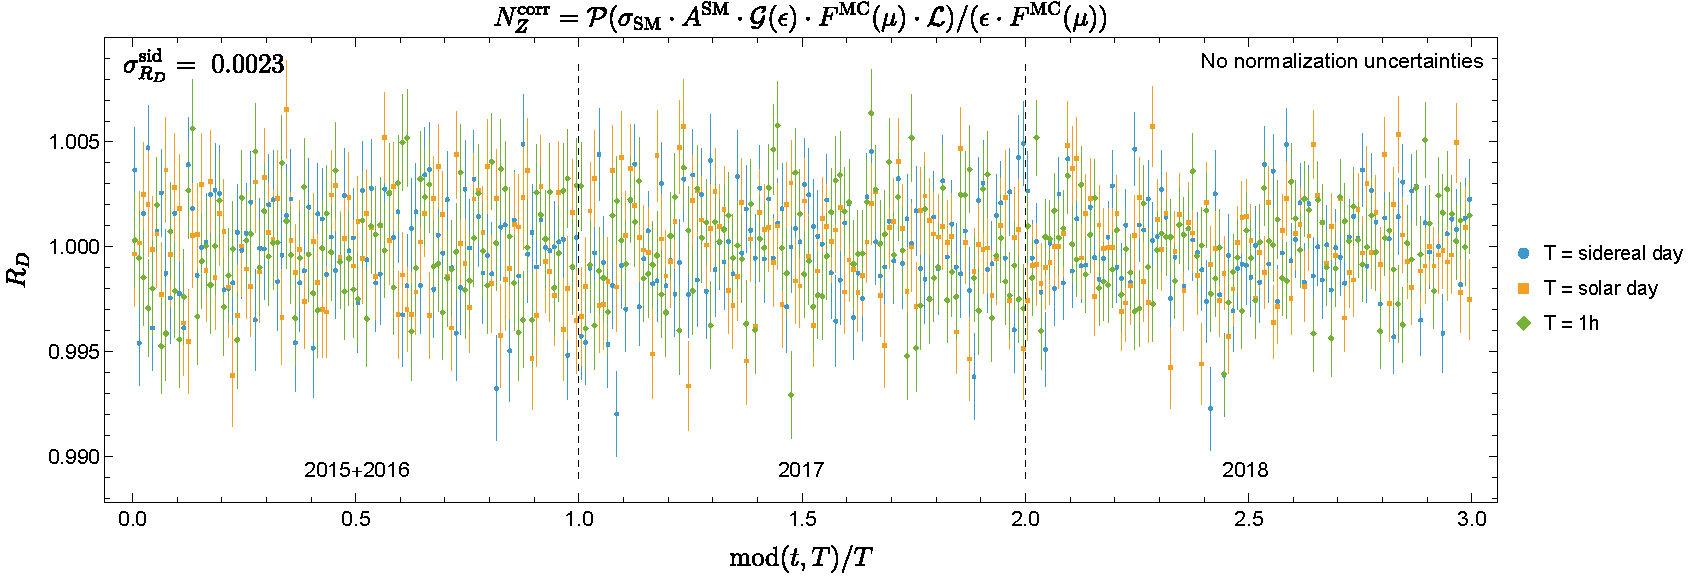
\includegraphics[width=\textwidth]{figs/Mathematica-oldchi2/xs(sigmaFID eps FMC)_noFMCErr_phase}
\caption{$R_D$ distribution for the toy study described in the text. In the upper right corner we show the standard deviation of the sidereal day distribution.}
\label{fig:RD_noFMCerrors}
\end{figure}

\begin{figure}[H]
\centering
\begin{minipage}[H]{0.49\textwidth}
    \vspace{1.6cm}
    \centering
    \begin{tabular}{|l|c|}
        \hline
        $d_u^{XZ}$ & $(0.5 \pm 4.0)\times 10^{-6}$ \\
        $d_u^{YZ}$ & $(-5.7 \pm 3.8)\times 10^{-6}$ \\
        $d_u^{XX-YY}$ & $(-2.4 \pm 2.0)\times 10^{-6}$ \\
        $d_u^{XY}$ & $(-1. \pm 9.5)\times 10^{-7}$ \\
        $c_u^{XZ}$ & $(0.4 \pm 3.1)\times 10^{-6}$ \\
        $c_u^{YZ}$ & $(-4.4 \pm 3.0)\times 10^{-6}$ \\
        $c_u^{XX-YY}$ & $(-1.9 \pm 1.5)\times 10^{-6}$ \\
        $c_u^{XY}$ & $(-0.7 \pm 7.4)\times 10^{-7}$ \\
        $c_d^{XZ}$ & $(0.2 \pm 1.4)\times 10^{-4}$ \\
        $c_d^{YZ}$ & $(-2.0 \pm 1.3)\times 10^{-4}$ \\
        $c_d^{XX-YY}$ & $(-8.3 \pm 6.8)\times 10^{-5}$ \\
        $c_d^{XY}$ & $(-0.3 \pm 3.3)\times 10^{-5}$ \\
                \hline
        \end{tabular}
\end{minipage}
\begin{minipage}[H]{0.49\textwidth}
    \vspace{0pt}
    \centering
   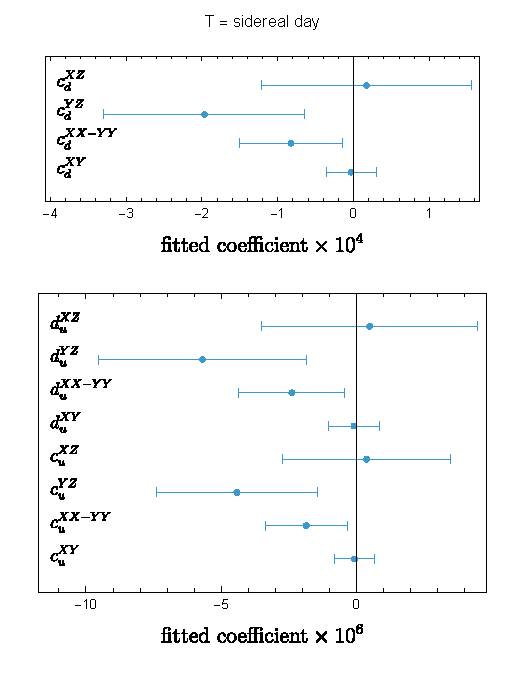
\includegraphics[width=\textwidth]{figs/Mathematica-oldchi2/xs(sigmaFID eps FMC)_noFMCErr_fit}
\end{minipage}
\caption{Fit results for the $N_Z = \sigma_\text{SM}\cdot A^\text{SM} \cdot \epsilon \cdot F^\text{MC}(\mu) \cdot {\cal L}$. No uncertainties on $F^\text{MC}(\mu)$ are included.}
\label{fig:RD_noFMCerrors_fits}
\end{figure}




\subsection{\texorpdfstring{
$N_Z^\text{corr} = \sigma_\text{fid} \cdot \epsilon \cdot F_\text{MC}(\mu)\cdot {\cal L}$ 
with $\delta \epsilon \neq 0$ and $\delta F^\text{MC}(\mu) \neq 0$}{NZcorr = sigmafid * epsilon * FMC * L with delta epsilon != 0 and delta FMC != 0}}
\label{ssec:all_errors_included}
%
We now repeat the study in Sec.~\ref{ssec:no_FMC_errors} but including uncertainties on $F^\text{MC}(\mu)$. This is the most accurate simulation of the expected $Z$ counts that we can produce. There are two effects that play a role: 
%
\begin{enumerate}
    \item The genuine uncertainty on the fitted $F^\text{MC}(\mu)$ function as shown in figure~4 of Ref.~\cite{ATL-DAPR-PUB-2021-001}.
    \item An uncertainty on the normalization which yields $\mu$ and which introduces a $\delta \mu = 1$ (or 1/2) which is 100\% correlated across all LBs in years 2015/2016, 2017 and 2018. 
\end{enumerate} 
%
As of now we do not have a parametrized version of the genuine $F^\text{MC}(\mu)$ uncertainty and we use $\delta \mu = 1$ in each LB as a proxy for the correct uncertainty. As can be seen in figure~4 of Ref.~\cite{ATL-DAPR-PUB-2021-001}, this procedure yields, in first approximation, the correct uncertainty (which, in any case, turns out to be subdominant compared to the uncertainty on the efficiency $\epsilon$). 

The simulated expected number of events and the corrected counts read:
%
\begin{align}
        N_Z (t)  & = {\cal P} \left( \sigma_\text{fid} \cdot {\cal G} (\epsilon,\delta\epsilon) \cdot F^\text{MC}({\cal G}(\mu,\delta \mu)) \cdot {\cal L}\right) , \label{eq:NZfull}\\
        N_Z^\text{corr} (t) & = \frac{N_Z(t)}{(\epsilon \pm \delta \epsilon) \cdot F^\text{MC}(\mu \pm \delta \mu)} .\label{eq:NZcorrfull}
    \end{align}
%
The double ratio $R_D$ is the constructed as in Eq.~(\ref{eq:RD}). The resulting distribution is shown in figure~\ref{fig:RD_Allerrors}. The standard deviation of the 100 bins for this example is $\sigma_{R_D} = 2.4 \times 10^{-3}$. Using the signal formulas discussed in Eqs.~\ref{eq:duXZ}-\ref{eq:cdXY}, we perform a fit to the 12 SME coefficients. The results are shown in figure~\ref{fig:RD_Allerrors_fits}. The central values are not zero because they have been obtained by a single Poisson sampling.

We see that the impact of including the uncertainty on $F^\text{MC}(\mu)$ is negligible. 

\begin{figure}[H]
\centering
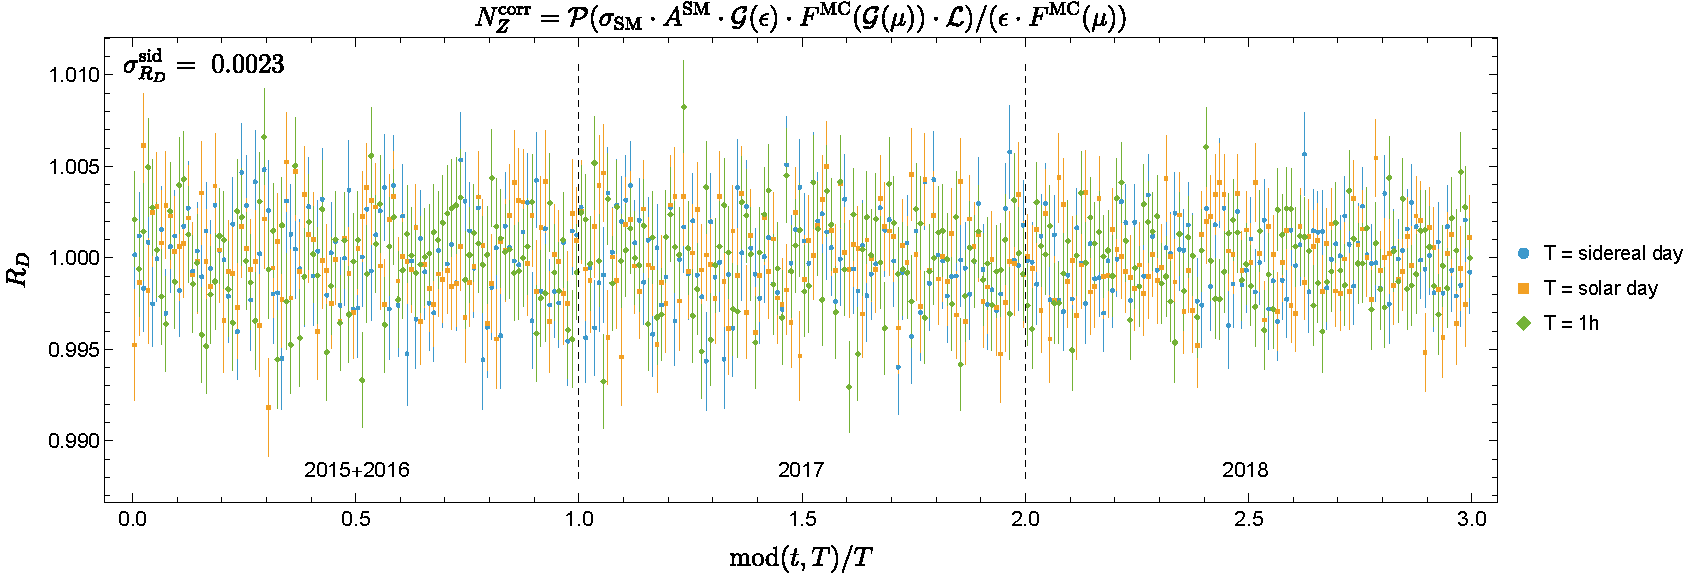
\includegraphics[width=\textwidth]{figs/Mathematica-oldchi2/xs(sigmaFID eps FMC)_phase}
\caption{$R_D$ distribution for the toy study described in the text. In the upper right corner we show the standard deviation of the sidereal day distribution. This is the most accurate simulation of $N_Z$ that we can produce.}
\label{fig:RD_Allerrors}
\end{figure}

\begin{figure}[H]
\centering
\begin{minipage}[H]{0.49\textwidth}
    \vspace{1.6cm}
    \centering
    \begin{tabular}{|l|c|}
        \hline
        $d_u^{XZ}$ & $(-0.7 \pm 4.8)\times 10^{-6}$ \\
        $d_u^{YZ}$ & $(-4.1 \pm 4.6)\times 10^{-6}$ \\
        $d_u^{XX-YY}$ & $(-1.1 \pm 2.4)\times 10^{-6}$ \\
        $d_u^{XY}$ & $(-1. \pm 11.)\times 10^{-7}$ \\
        $c_u^{XZ}$ & $(-0.5 \pm 3.7)\times 10^{-6}$ \\
        $c_u^{YZ}$ & $(-3.2 \pm 3.6)\times 10^{-6}$ \\
        $c_u^{XX-YY}$ & $(-0.8 \pm 1.8)\times 10^{-6}$ \\
        $c_u^{XY}$ & $(-1.0 \pm 8.9)\times 10^{-7}$ \\
        $c_d^{XZ}$ & $(-0.2 \pm 1.7)\times 10^{-4}$ \\
        $c_d^{YZ}$ & $(-1.4 \pm 1.6)\times 10^{-4}$ \\
        $c_d^{XX-YY}$ & $(-3.7 \pm 8.1)\times 10^{-5}$ \\
        $c_d^{XY}$ & $(-0.4 \pm 4.0)\times 10^{-5}$ \\
                                \hline
        \end{tabular}
\end{minipage}
\begin{minipage}[H]{0.49\textwidth}
    \vspace{0pt}
    \centering
   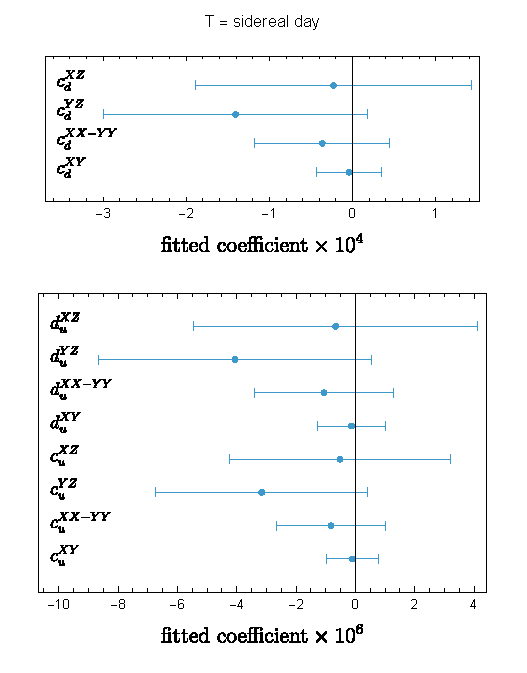
\includegraphics[width=\textwidth]{figs/Mathematica-oldchi2/xs(sigmaFID eps FMC)_fit}
\end{minipage}
\caption{Fit results for the $N_Z = \sigma_\text{SM}\cdot A^\text{SM} \cdot \epsilon \cdot F^\text{MC}(\mu) \cdot {\cal L}$. All sources of uncertainties are included. These results are based on the most accurate simulation of $N_Z$ that we can produce.}
\label{fig:RD_Allerrors_fits}
\end{figure}

\begin{figure}[H]
\centering
\includegraphics[width=\textwidth]{figs/Mathematica-oldchi2/NZ_over_time.pdf}
\caption{Expected number of $Z$ events (before efficiencies corrections) per LB. The LBs are time ordered.}
\label{fig:NZ_over_time}
\end{figure}

\clearpage
\section{Double ratio simulation studies: single sampling with signal injection}
\label{sec:double_ratio_injection_studies}
In this section we perform various signal injection tests. We only consider the double ratio constructed as in section~\ref{ssec:all_errors_included} (i.e. with all sources of uncertainties taken into account). We consider in turn the injection of a fairly large coefficient ($d_u^{YZ} = 1.35 \times 10^{-4}$) and injected it both with a sidereal and solar phase. The former corresponds to a possible signal while the latter simulates a potential day/night effect. The purposes of these studies are:
\begin{enumerate}
    \item Test to what extent we are able to recover the signal using our 100 bins fitting procedure.
    \item Test to what extent one single scrambling of the time stamps erases the signal. This is essential for proving the feasibility of a partial unblinding of the data (i.e. using the observed $Z$ counts but scrambling the time stamps).
    \item Test the extent of the solar/sidereal phase signal cross contamination. How large of a sidereal coefficient is observed if a solar phase signal is injected (and vice versa). 
    \item Test the size of the fitted coefficient as a function of the testing phase. 
\end{enumerate}
%

\subsection{Sidereal phase signal injection: recovery test}
\label{ssec:SiderealInjectionRecovery}
%
The construction of a simulated set of $Z$ counts with an injected sideral signal is achieved by simply replacing the SM fiducial cross section in Eqs.~(\ref{eq:NZfull}) and (\ref{eq:NZcorrfull}):
%
\begin{align}
    \sigma_\text{fid} = A^\text{SM} \sigma_\text{SM}^\text{NNLO} 
    \longrightarrow
    \sigma_\text{fid} \left[ 1 + d_u^{YZ} \big[ a \cos (\omega_\oplus T_\oplus) + b \sin (\omega_\oplus T_\oplus) \big] \right]
\end{align}
%
where the numerical values for $a$ and $b$ are taken from Eq.~(\ref{eq:duYZnum}). For a solar signal we use the same formula but replace the sidereal frequency $\omega_\oplus = 2\pi/T_\text{sidereal}$ with $\omega_\odot = 2\pi/T_\text{solar} = 2\pi/(24\; \text{hr})$. The $R_D$ distribution and the fit results for a sidereal, solar and 1 hr testing phase are presented in figures~\ref{fig:RD_sidereal_signal}, \ref{fig:RD_sidereal_signal_fits_sidsol} and \ref{fig:RD_sidereal_signal_fits_1h}. 

Several comments are in order:
\begin{itemize}
\item Using the sidereal testing phase, we extract $\left[d_u^{YZ}\right]_\text{fit} = (1.25 \pm 0.05)\times 10^{-4}$ which is quite compatible with the injected signal  $\left[d_u^{YZ}\right]_\text{injected} = 1.35 \times 10^{-4}$.
\item Using the sidereal testing phase, we find large reconstructed signals for all $YZ$ coefficients (and not only for $d_u^{YZ}$) because the time structure induced by these coefficients is identical (up to an overall rescaling factor). 
\item Using the sidereal testing phases, no coefficient other than the $YZ$ ones deviates from zero. Because of linearity, this demonstrates that, if multiple coefficients are present (e.g. a $YZ$ and an $XY$), they can all be identified (of course, we cannot distinguish between $c_d$, $c_u$ and $d_u$).
\item As can be seen in the right side of figure~\ref{fig:RD_sidereal_signal_fits_sidsol}, a large sidereal signal will induce (smaller) but still sizable solar day effects. 
\end{itemize}

\begin{figure}[H]
\centering
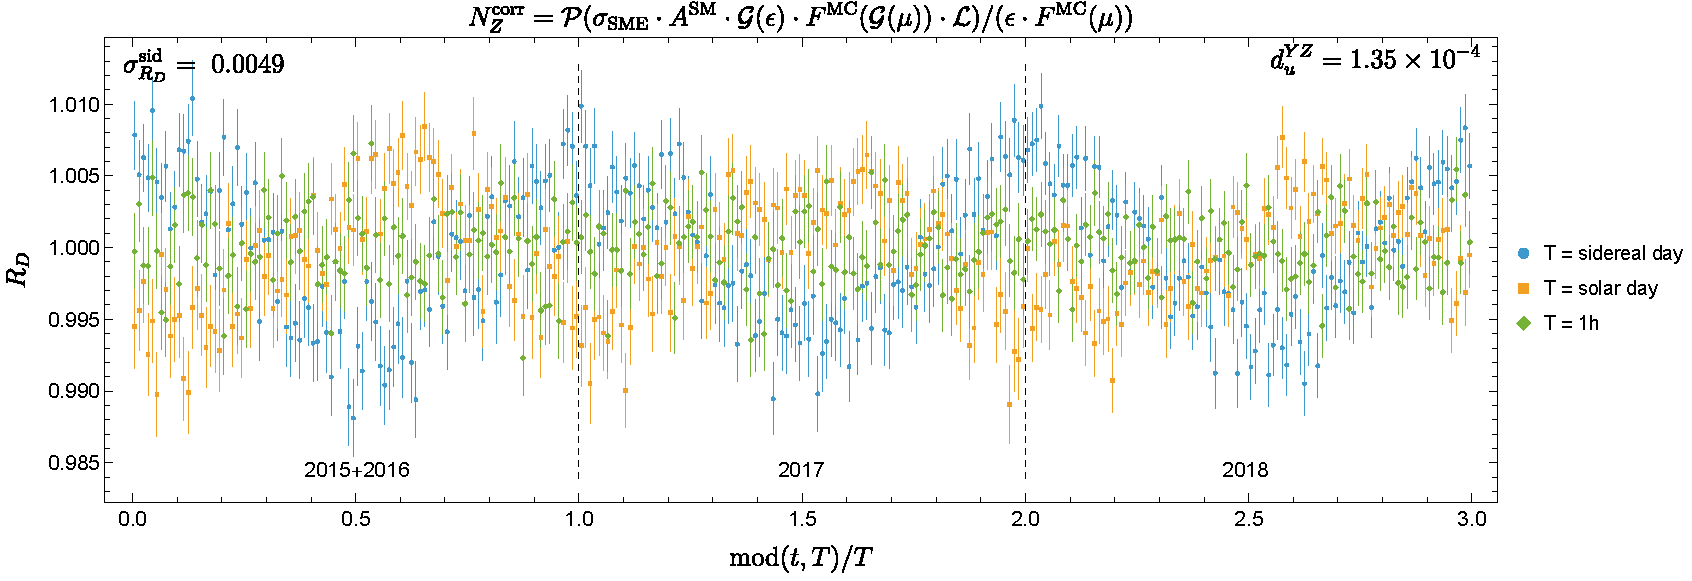
\includegraphics[width=\textwidth]{figs/Mathematica-oldchi2/xs(sigmaFIDSME eps FMC)_phase}
\caption{$R_D$ distribution with a sidereal signal injection ($d_u^{YZ} = 1.35 \times 10^{-4}$). In the upper right corner we show the standard deviation of the sidereal day distribution.}
\label{fig:RD_sidereal_signal}
\end{figure}

\begin{figure}[H]
\centering
\begin{minipage}[H]{\textwidth}
    \vspace{0pt}
    \centering
   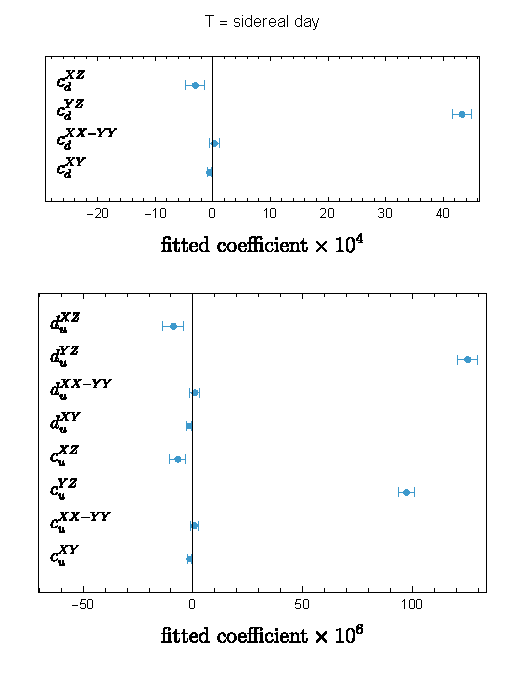
\includegraphics[width=0.49\textwidth]{figs/Mathematica-oldchi2/xs(sigmaFIDSME eps FMC)_fit_sday}
   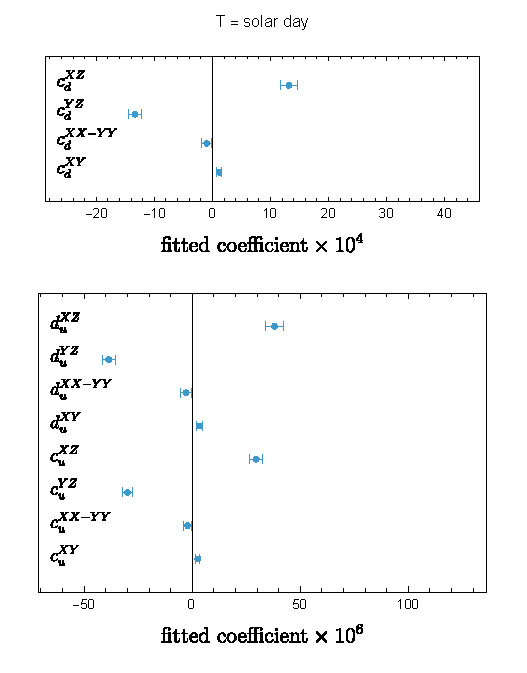
\includegraphics[width=0.49\textwidth]{figs/Mathematica-oldchi2/xs(sigmaFIDSME eps FMC)_fit_day}
\end{minipage}
\begin{minipage}[H]{\textwidth}
    \vspace{1.6cm}
    \centering
    \begin{tabular}{|l|c|}
        \hline
        $d_u^{XZ}$ & $(-8.9 \pm 4.8)\times 10^{-6}$ \\
        $d_u^{YZ}$ & $(1.252 \pm 0.046)\times 10^{-4}$ \\
        $d_u^{XX-YY}$ & $(0.9 \pm 2.4)\times 10^{-6}$ \\
        $d_u^{XY}$ & $(-1.8 \pm 1.1)\times 10^{-6}$ \\
        $c_u^{XZ}$ & $(-6.9 \pm 3.7)\times 10^{-6}$ \\
        $c_u^{YZ}$ & $(9.73 \pm 0.36)\times 10^{-5}$ \\
        $c_u^{XX-YY}$ & $(0.7 \pm 1.8)\times 10^{-6}$ \\
        $c_u^{XY}$ & $(-1.40 \pm 0.89)\times 10^{-6}$ \\
        $c_d^{XZ}$ & $(-3.1 \pm 1.7)\times 10^{-4}$ \\
        $c_d^{YZ}$ & $(4.33 \pm 0.16)\times 10^{-3}$ \\
        $c_d^{XX-YY}$ & $(3.0 \pm 8.1)\times 10^{-5}$ \\
        $c_d^{XY}$ & $(-6.2 \pm 4.0)\times 10^{-5}$ \\
                \hline
        \end{tabular}
        \;\;\;\;\;\;\;\;\;\;\;\;\;\;\;\;\;\;
    \begin{tabular}{|l|c|}
        \hline
        $d_u^{XZ}$ & $(3.81 \pm 0.41)\times 10^{-5}$ \\
        $d_u^{YZ}$ & $(-3.86 \pm 0.32)\times 10^{-5}$ \\
        $d_u^{XX-YY}$ & $(-2.8 \pm 2.4)\times 10^{-6}$ \\
        $d_u^{XY}$ & $(3.4 \pm 1.2)\times 10^{-6}$ \\
        $c_u^{XZ}$ & $(2.96 \pm 0.32)\times 10^{-5}$ \\
        $c_u^{YZ}$ & $(-3.00 \pm 0.25)\times 10^{-5}$ \\
        $c_u^{XX-YY}$ & $(-2.2 \pm 1.9)\times 10^{-6}$ \\
        $c_u^{XY}$ & $(2.61 \pm 0.90)\times 10^{-6}$ \\
        $c_d^{XZ}$ & $(1.32 \pm 0.14)\times 10^{-3}$ \\
        $c_d^{YZ}$ & $(-1.33 \pm 0.11)\times 10^{-3}$ \\
        $c_d^{XX-YY}$ & $(-9.8 \pm 8.4)\times 10^{-5}$ \\
        $c_d^{XY}$ & $(1.16 \pm 0.40)\times 10^{-4}$ \\
                        \hline
        \end{tabular}
\end{minipage}
\caption{Sidereal signal injection test ($d_u^{YZ} = 1.35 \times 10^{-4}$): fit results for sidereal (left) and solar (right) testing phases.}
\label{fig:RD_sidereal_signal_fits_sidsol}
\end{figure}

\begin{figure}[H]
\centering
\begin{minipage}[H]{0.49\textwidth}
    \vspace{1.6cm}
    \centering
    \begin{tabular}{|l|c|}
        \hline
        $d_u^{XZ}$ & $(-5.0 \pm 4.8)\times 10^{-6}$ \\
        $d_u^{YZ}$ & $(2.9 \pm 4.8)\times 10^{-6}$ \\
        $d_u^{XX-YY}$ & $(1.3 \pm 2.5)\times 10^{-6}$ \\
        $d_u^{XY}$ & $(6. \pm 12.)\times 10^{-7}$ \\
        $c_u^{XZ}$ & $(-3.9 \pm 3.7)\times 10^{-6}$ \\
        $c_u^{YZ}$ & $(2.3 \pm 3.7)\times 10^{-6}$ \\
        $c_u^{XX-YY}$ & $(1.0 \pm 1.9)\times 10^{-6}$ \\
        $c_u^{XY}$ & $(4.9 \pm 9.5)\times 10^{-7}$ \\
        $c_d^{XZ}$ & $(-1.7 \pm 1.7)\times 10^{-4}$ \\
        $c_d^{YZ}$ & $(1.0 \pm 1.7)\times 10^{-4}$ \\
        $c_d^{XX-YY}$ & $(4.5 \pm 8.5)\times 10^{-5}$ \\
        $c_d^{XY}$ & $(2.2 \pm 4.2)\times 10^{-5}$ \\
        \hline
        \end{tabular}
\end{minipage}
\begin{minipage}[H]{0.49\textwidth}
    \vspace{0pt}
    \centering
   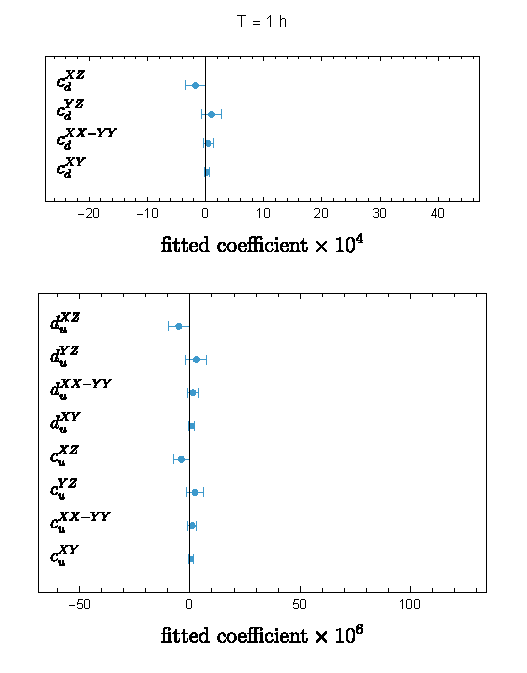
\includegraphics[width=\textwidth]{figs/Mathematica-oldchi2/xs(sigmaFIDSME eps FMC)_fit_1h}
\end{minipage}
\caption{Sidereal signal injection test ($d_u^{YZ} = 1.35 \times 10^{-4}$): fit results for 1 hr testing phase.}
\label{fig:RD_sidereal_signal_fits_1h}
\end{figure}

\subsection{Sidereal phase signal injection: scrambling}
\label{ssec:SiderealInjectionScrambling}
%
In figures~\ref{fig:RD_sidereal_signal_scrambled} and \ref{fig:RD_sidereal_signal_scrambled_fits_sidsol}, we demonstrate that a random scrambling of all time stamps is sufficient to completely erase the presence of a strong sidereal signal. Note that, after scrambling, the standard deviation over the 100 bins in $R_D$ drops from 0.0049 to 0.0026 (which is typical of a SM simulation without signal injection). 

\begin{figure}[H]
\centering
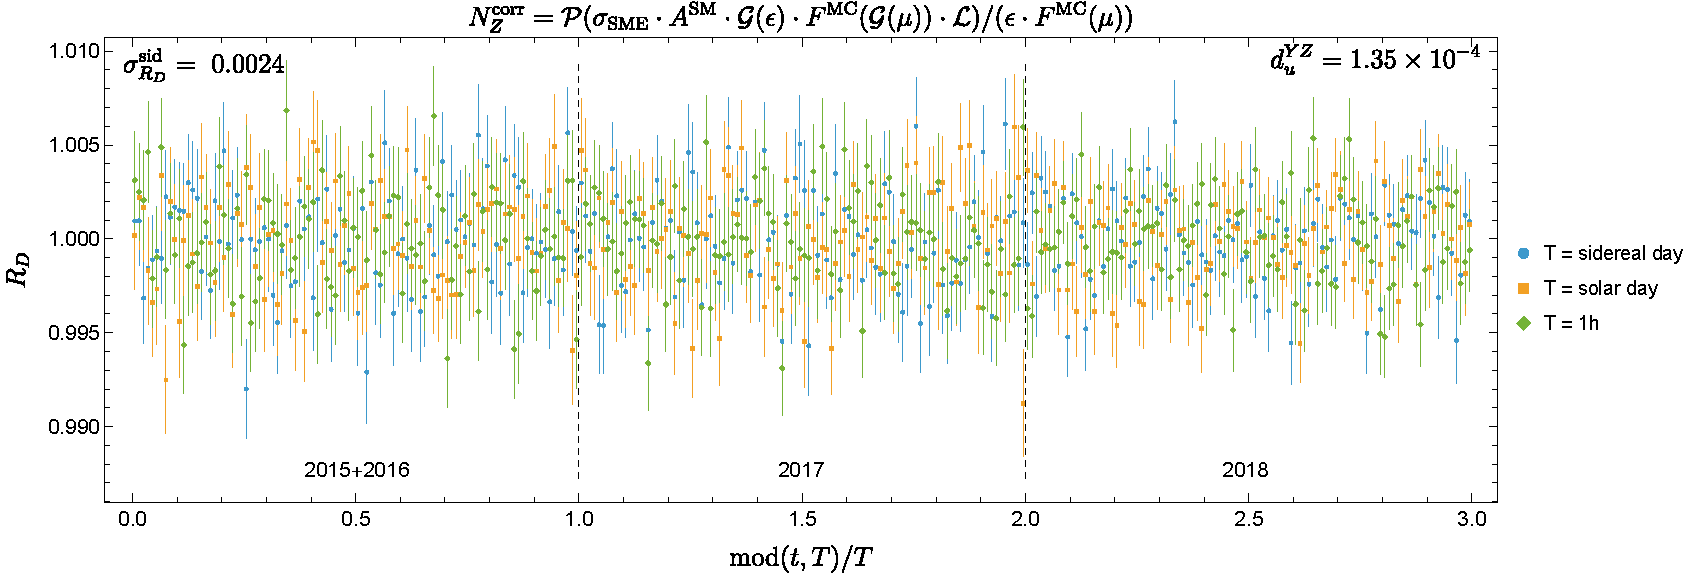
\includegraphics[width=\textwidth]{figs/Mathematica-oldchi2/xs(sigmaFIDSME eps FMC)_randomized_phase}
\caption{$R_D$ distribution with a sidereal signal injection ($d_u^{YZ} = 1.35 \times 10^{-4}$) after one scrambling. In the upper right corner we show the standard deviation of the sidereal day distribution.}
\label{fig:RD_sidereal_signal_scrambled}
\end{figure}


\begin{figure}[H]
\centering
\begin{minipage}[H]{\textwidth}
    \vspace{0pt}
    \centering
   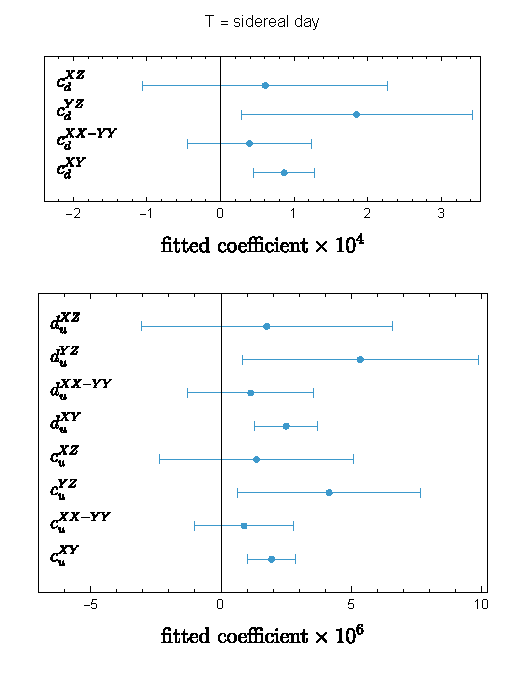
\includegraphics[width=0.49\textwidth]{figs/Mathematica-oldchi2/xs(sigmaFIDSME eps FMC)_randomized_fit_sday}
   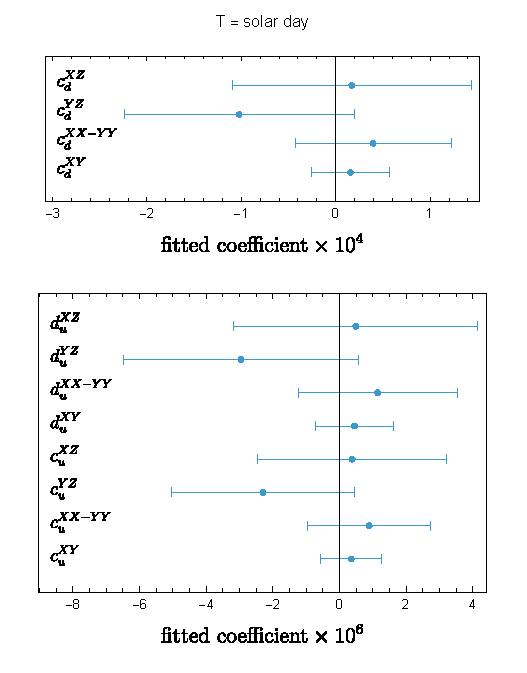
\includegraphics[width=0.49\textwidth]{figs/Mathematica-oldchi2/xs(sigmaFIDSME eps FMC)_randomized_fit_day}
\end{minipage}
\begin{minipage}[H]{\textwidth}
    \vspace{1.6cm}
    \centering
    \begin{tabular}{|l|c|}
        \hline
        $d_u^{XZ}$ & $(-8.9 \pm 4.8)\times 10^{-6}$ \\
        $d_u^{YZ}$ & $(1.252 \pm 0.046)\times 10^{-4}$ \\
        $d_u^{XX-YY}$ & $(0.9 \pm 2.4)\times 10^{-6}$ \\
        $d_u^{XY}$ & $(-1.8 \pm 1.1)\times 10^{-6}$ \\
        $c_u^{XZ}$ & $(-6.9 \pm 3.7)\times 10^{-6}$ \\
        $c_u^{YZ}$ & $(9.73 \pm 0.36)\times 10^{-5}$ \\
        $c_u^{XX-YY}$ & $(0.7 \pm 1.8)\times 10^{-6}$ \\
        $c_u^{XY}$ & $(-1.40 \pm 0.89)\times 10^{-6}$ \\
        $c_d^{XZ}$ & $(-3.1 \pm 1.7)\times 10^{-4}$ \\
        $c_d^{YZ}$ & $(4.33 \pm 0.16)\times 10^{-3}$ \\
        $c_d^{XX-YY}$ & $(3.0 \pm 8.1)\times 10^{-5}$ \\
        $c_d^{XY}$ & $(-6.2 \pm 4.0)\times 10^{-5}$ \\
                \hline
        \end{tabular}
        \;\;\;\;\;\;\;\;\;\;\;\;\;\;\;\;\;\;
    \begin{tabular}{|l|c|}
        \hline
        $d_u^{XZ}$ & $(3.81 \pm 0.41)\times 10^{-5}$ \\
        $d_u^{YZ}$ & $(-3.86 \pm 0.32)\times 10^{-5}$ \\
        $d_u^{XX-YY}$ & $(-2.8 \pm 2.4)\times 10^{-6}$ \\
        $d_u^{XY}$ & $(3.4 \pm 1.2)\times 10^{-6}$ \\
        $c_u^{XZ}$ & $(2.96 \pm 0.32)\times 10^{-5}$ \\
        $c_u^{YZ}$ & $(-3.00 \pm 0.25)\times 10^{-5}$ \\
        $c_u^{XX-YY}$ & $(-2.2 \pm 1.9)\times 10^{-6}$ \\
        $c_u^{XY}$ & $(2.61 \pm 0.90)\times 10^{-6}$ \\
        $c_d^{XZ}$ & $(1.32 \pm 0.14)\times 10^{-3}$ \\
        $c_d^{YZ}$ & $(-1.33 \pm 0.11)\times 10^{-3}$ \\
        $c_d^{XX-YY}$ & $(-9.8 \pm 8.4)\times 10^{-5}$ \\
        $c_d^{XY}$ & $(1.16 \pm 0.40)\times 10^{-4}$ \\
                        \hline
        \end{tabular}
\end{minipage}
\caption{Sidereal signal injection test ($d_u^{YZ} = 1.35 \times 10^{-4}$) after one scrambling of all time stamps: fit results for sidereal (left) and solar (right) testing phases.}
\label{fig:RD_sidereal_signal_scrambled_fits_sidsol}
\end{figure}



\subsection{Sidereal phase signal injection: scan over the testing phase}
\label{ssec:SiderealInjectionScan}
%
In this section we study, as a function of the testing phase, the extraction of the coefficient $d_u^{YZ}$ from a sample in which a $d_u^{YZ} = 1.35 \times 10^{-4}$ sidereal signal has been injected. The results of this test is presented in figure~\ref{fig:RD_sidereal_signal_scan} (the four lower panels focus on the restricted [23 hr, 25 hr] range). Around the sidereal and solar phases we scan the testing phase with a granularity of 1 min (going below this is problematic because the average LB duration is about 1 min). 

This analysis suggests a possible strategy to decide whether a positive observation is a genuine sidereal signal or a day/night effect: just check whether the largest extracted coefficient is the output of a sidereal or solar testing phase. 

\begin{figure}[H]
\centering
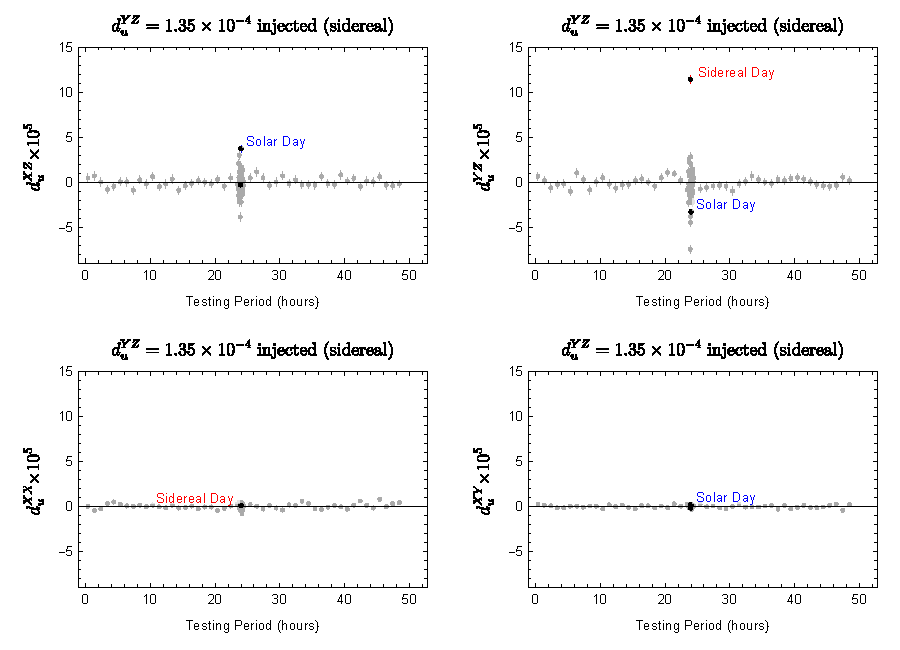
\includegraphics[width=0.8\textwidth]{figs/Mathematica-oldchi2/fit_duYZinjected_scan-wide}
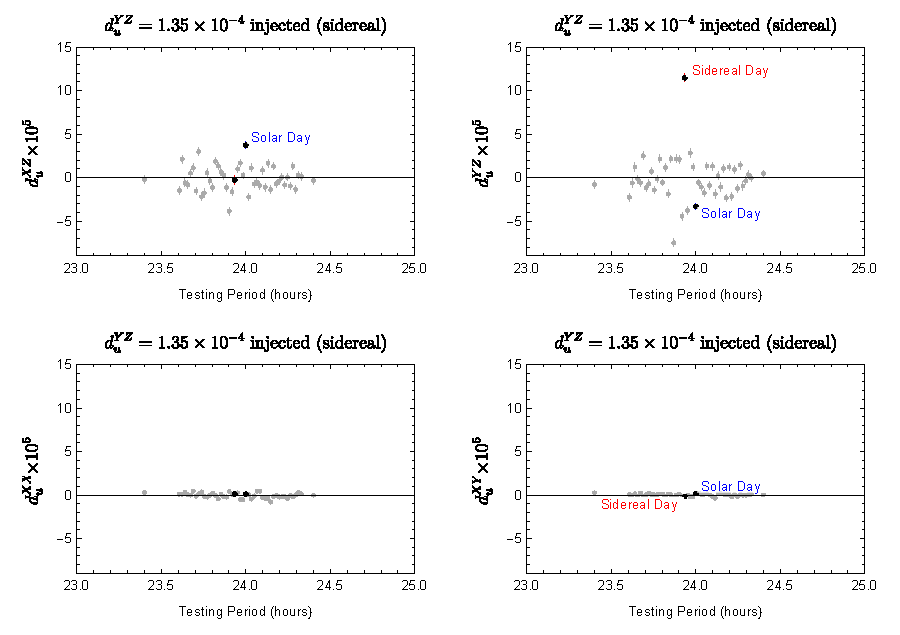
\includegraphics[width=0.8\textwidth]{figs/Mathematica-oldchi2/fit_duYZinjected_scan-narrow}
\caption{Sidereal signal injection ($d_u^{YZ} = 1.35 \times 10^{-4}$). Fit for the $d_u^{YZ}$ coefficient as a function of the testing phase. Red and blue fits correspond to the sidereal and solar testing phases.}
\label{fig:RD_sidereal_signal_scan}
\end{figure}



\subsection{Solar phase signal injection: recovery test}
\label{ssec:SolarInjectionRecovery}
%
Same as section~\ref{ssec:SiderealInjectionRecovery} but with a solar signal injected. Results are presented in figures~\ref{fig:RD_solar_signal}, \ref{fig:RD_solar_signal_fits_sidsol} and \ref{fig:RD_solar_signal_fits_1h}. \textcolor{red}{There is one feature of these results which I do not understand. Using a solar testing phase I find $\left[ d_u^{YZ}\right]_\text{fit} = (6.4 \pm 0.3) \times 10^{-5}$ which is a factor two smaller than the injected one.}

\begin{figure}[H]
\centering
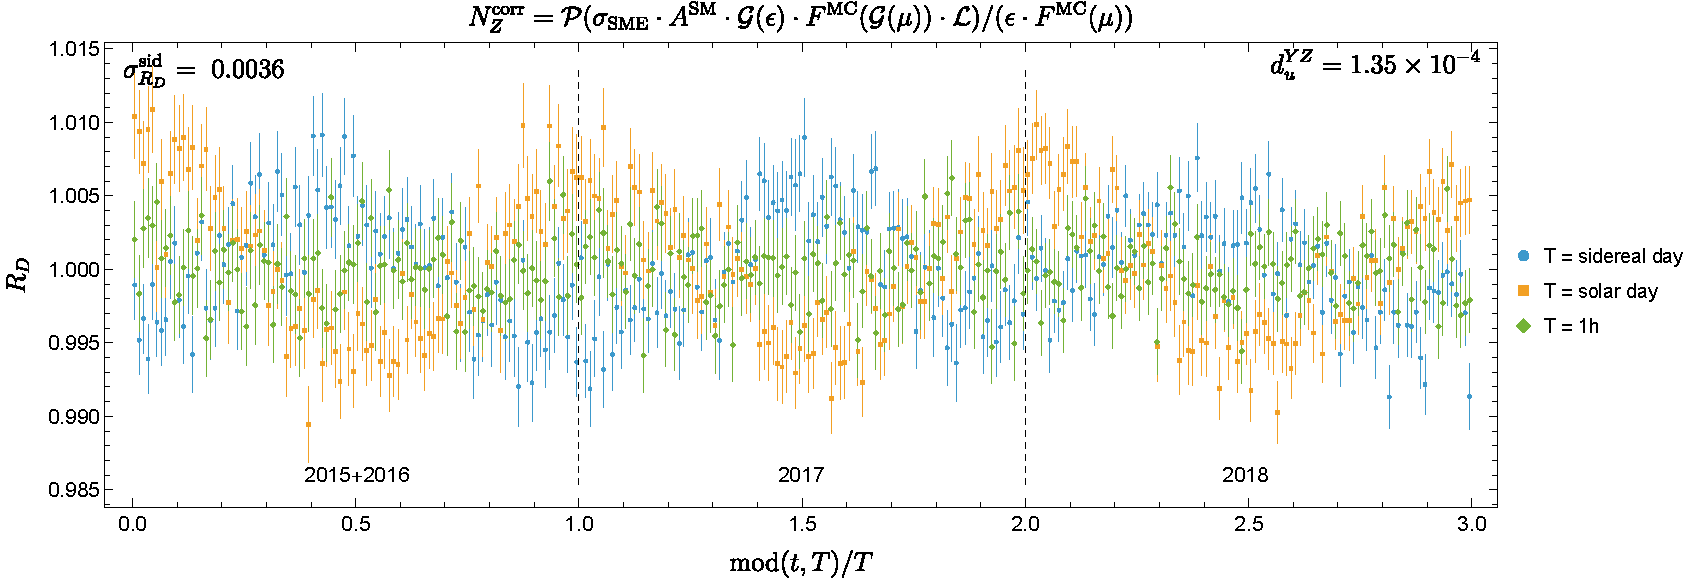
\includegraphics[width=\textwidth]{figs/Mathematica-oldchi2/xs(sigmaFIDSMEsolar eps FMC)_phase}
\caption{$R_D$ distribution with a solar signal injection ($d_u^{YZ} = 1.35 \times 10^{-4}$). In the upper right corner we show the standard deviation of the sidereal day distribution.}
\label{fig:RD_solar_signal}
\end{figure}

\begin{figure}[H]
\centering
\begin{minipage}[H]{\textwidth}
    \vspace{0pt}
    \centering
   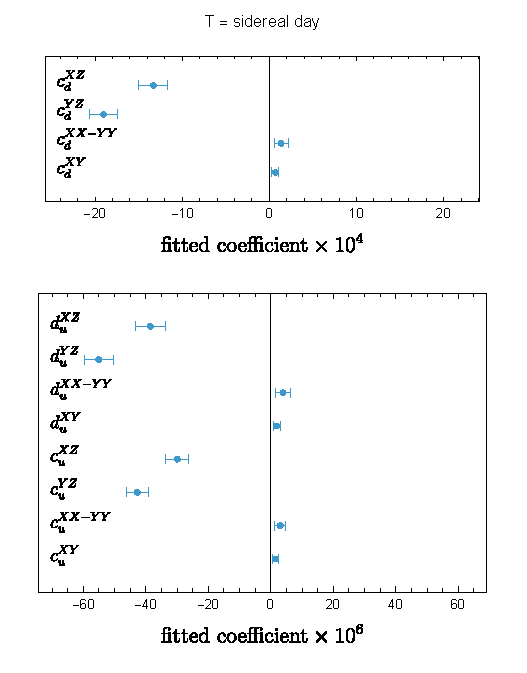
\includegraphics[width=0.49\textwidth]{figs/Mathematica-oldchi2/xs(sigmaFIDSMEsolar eps FMC)_fit_sday}
   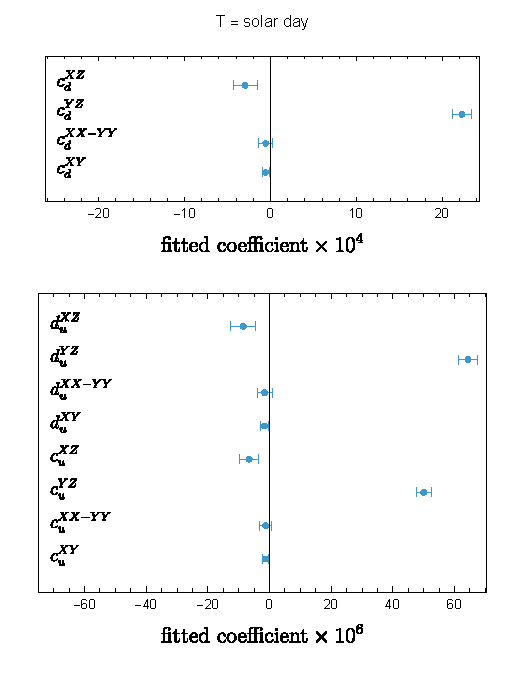
\includegraphics[width=0.49\textwidth]{figs/Mathematica-oldchi2/xs(sigmaFIDSMEsolar eps FMC)_fit_day}
\end{minipage}
\begin{minipage}[H]{\textwidth}
    \vspace{1.6cm}
    \centering
    \begin{tabular}{|l|c|}
        \hline
$d_u^{XZ}$ & $(-3.85 \pm 0.48)\times 10^{-5}$ \\
$d_u^{YZ}$ & $(-5.50 \pm 0.46)\times 10^{-5}$ \\
$d_u^{XX-YY}$ & $(3.9 \pm 2.3)\times 10^{-6}$ \\
$d_u^{XY}$ & $(1.9 \pm 1.1)\times 10^{-6}$ \\
$c_u^{XZ}$ & $(-2.99 \pm 0.37)\times 10^{-5}$ \\
$c_u^{YZ}$ & $(-4.27 \pm 0.36)\times 10^{-5}$ \\
$c_u^{XX-YY}$ & $(3.0 \pm 1.8)\times 10^{-6}$ \\
$c_u^{XY}$ & $(1.51 \pm 0.89)\times 10^{-6}$ \\
$c_d^{XZ}$ & $(-1.33 \pm 0.17)\times 10^{-3}$ \\
$c_d^{YZ}$ & $(-1.90 \pm 0.16)\times 10^{-3}$ \\
$c_d^{XX-YY}$ & $(1.35 \pm 0.81)\times 10^{-4}$ \\
$c_d^{XY}$ & $(6.7 \pm 4.0)\times 10^{-5}$ \\
                        \hline
        \end{tabular}
        \;\;\;\;\;\;\;\;\;\;\;\;\;\;\;\;\;\;
    \begin{tabular}{|l|c|}
        \hline
$d_u^{XZ}$ & $(-8.5 \pm 4.1)\times 10^{-6}$ \\
$d_u^{YZ}$ & $(6.44 \pm 0.32)\times 10^{-5}$ \\
$d_u^{XX-YY}$ & $(-1.6 \pm 2.4)\times 10^{-6}$ \\
$d_u^{XY}$ & $(-1.6 \pm 1.2)\times 10^{-6}$ \\
$c_u^{XZ}$ & $(-6.6 \pm 3.2)\times 10^{-6}$ \\
$c_u^{YZ}$ & $(5.00 \pm 0.25)\times 10^{-5}$ \\
$c_u^{XX-YY}$ & $(-1.2 \pm 1.9)\times 10^{-6}$ \\
$c_u^{XY}$ & $(-1.25 \pm 0.90)\times 10^{-6}$ \\
$c_d^{XZ}$ & $(-2.9 \pm 1.4)\times 10^{-4}$ \\
$c_d^{YZ}$ & $(2.23 \pm 0.11)\times 10^{-3}$ \\
$c_d^{XX-YY}$ & $(-5.5 \pm 8.4)\times 10^{-5}$ \\
$c_d^{XY}$ & $(-5.6 \pm 4.0)\times 10^{-5}$ \\
                                \hline
        \end{tabular}
\end{minipage}
\caption{Solar signal injection test ($d_u^{YZ} = 1.35 \times 10^{-4}$): fit results for sidereal (left) and solar (right) testing phases.}
\label{fig:RD_solar_signal_fits_sidsol}
\end{figure}


\begin{figure}[H]
\centering
\begin{minipage}[H]{0.49\textwidth}
    \vspace{1.6cm}
    \centering
    \begin{tabular}{|l|c|}
        \hline
$d_u^{XZ}$ & $(5.1 \pm 4.8)\times 10^{-6}$ \\
$d_u^{YZ}$ & $(6.8 \pm 4.8)\times 10^{-6}$ \\
$d_u^{XX-YY}$ & $(1.2 \pm 2.5)\times 10^{-6}$ \\
$d_u^{XY}$ & $(11. \pm 12.)\times 10^{-7}$ \\
$c_u^{XZ}$ & $(4.0 \pm 3.7)\times 10^{-6}$ \\
$c_u^{YZ}$ & $(5.3 \pm 3.7)\times 10^{-6}$ \\
$c_u^{XX-YY}$ & $(0.9 \pm 1.9)\times 10^{-6}$ \\
$c_u^{XY}$ & $(8.8 \pm 9.5)\times 10^{-7}$ \\
$c_d^{XZ}$ & $(1.8 \pm 1.7)\times 10^{-4}$ \\
$c_d^{YZ}$ & $(2.4 \pm 1.7)\times 10^{-4}$ \\
$c_d^{XX-YY}$ & $(4.1 \pm 8.5)\times 10^{-5}$ \\
$c_d^{XY}$ & $(3.9 \pm 4.2)\times 10^{-5}$ \\
        \hline
        \end{tabular}
\end{minipage}
\begin{minipage}[H]{0.49\textwidth}
    \vspace{0pt}
    \centering
   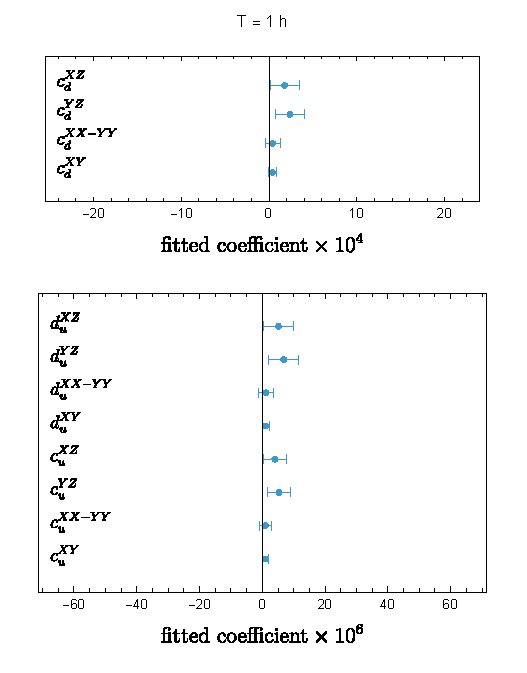
\includegraphics[width=\textwidth]{figs/Mathematica-oldchi2/xs(sigmaFIDSMEsolar eps FMC)_fit_1h}
\end{minipage}
\caption{Solar signal injection test ($d_u^{YZ} = 1.35 \times 10^{-4}$): fit results for 1 hr testing phase.}
\label{fig:RD_solar_signal_fits_1h}
\end{figure}


\subsection{Solar phase signal injection: scrambling}
\label{ssec:SolarInjectionScrambling}
%
In figures~\ref{fig:RD_solar_signal_scrambled} and \ref{fig:RD_solar_signal_scrambled_fits_sidsol}, we demonstrate that a random scrambling of all time stamps is sufficient to completely erase the presence of a strong solar signal.


\begin{figure}[H]
\centering
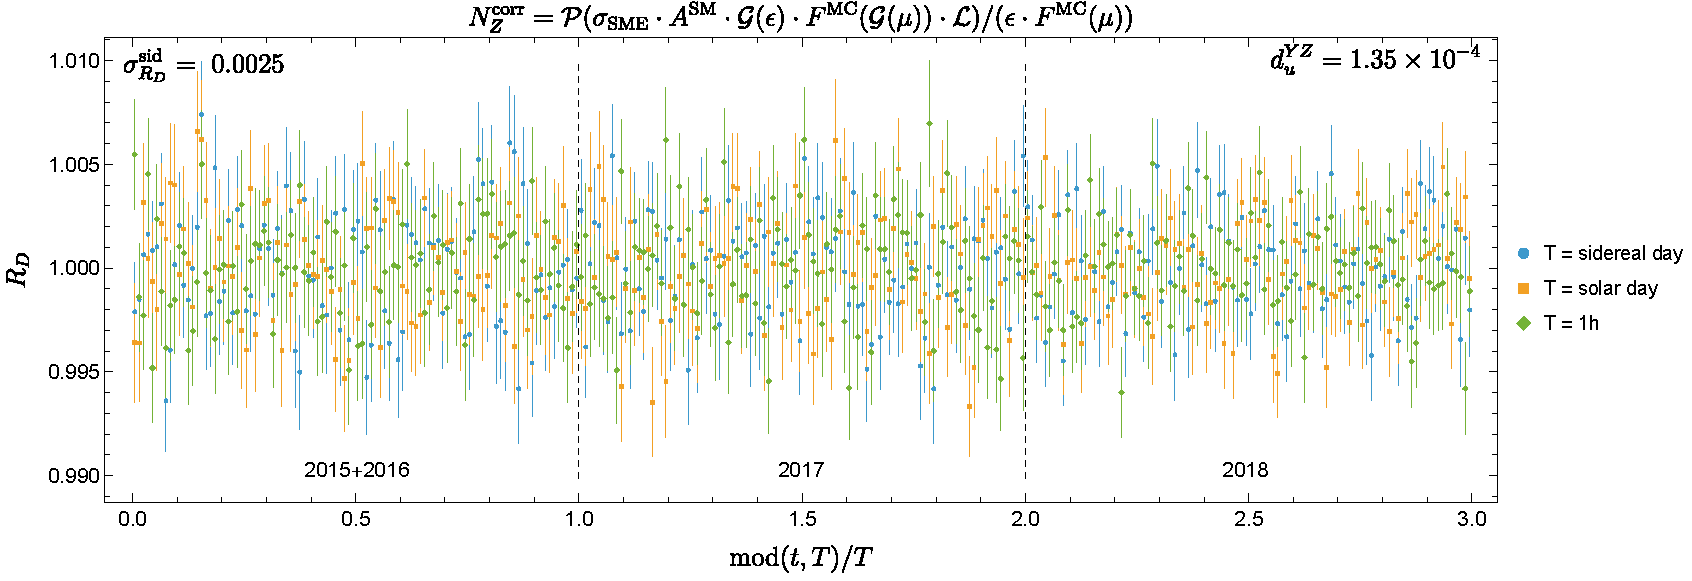
\includegraphics[width=\textwidth]{figs/Mathematica-oldchi2/xs(sigmaFIDSMEsolar eps FMC)_randomized_phase}
\caption{$R_D$ distribution with a solar signal injection ($d_u^{YZ} = 1.35 \times 10^{-4}$) after one scrambling. In the upper right corner we show the standard deviation of the sidereal day distribution.}
\label{fig:RD_solar_signal_scrambled}
\end{figure}


\begin{figure}[H]
\centering
\begin{minipage}[H]{\textwidth}
    \vspace{0pt}
    \centering
   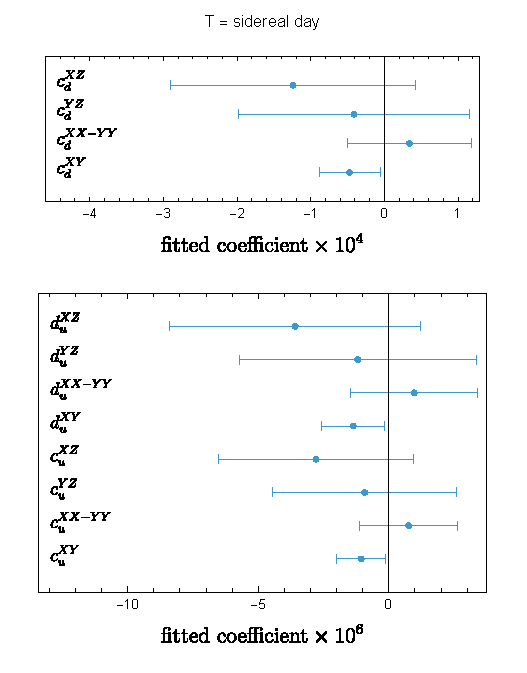
\includegraphics[width=0.49\textwidth]{figs/Mathematica-oldchi2/xs(sigmaFIDSMEsolar eps FMC)_randomized_fit_sday}
   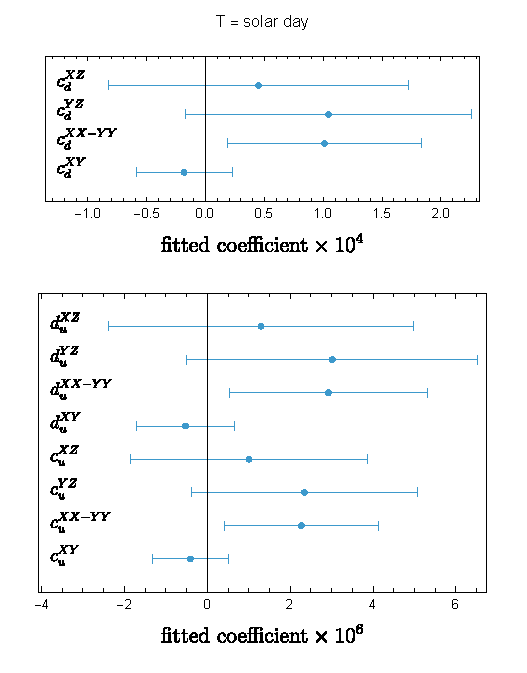
\includegraphics[width=0.49\textwidth]{figs/Mathematica-oldchi2/xs(sigmaFIDSMEsolar eps FMC)_randomized_fit_day}
\end{minipage}
\begin{minipage}[H]{\textwidth}
    \vspace{1.6cm}
    \centering
    \begin{tabular}{|l|c|}
        \hline
$d_u^{XZ}$ & $(-3.6 \pm 4.8)\times 10^{-6}$ \\
$d_u^{YZ}$ & $(-1.2 \pm 4.5)\times 10^{-6}$ \\
$d_u^{XX-YY}$ & $(1. \pm 2.4)\times 10^{-6}$ \\
$d_u^{XY}$ & $(-14. \pm 12.)\times 10^{-7}$ \\
$c_u^{XZ}$ & $(-2.8 \pm 3.7)\times 10^{-6}$ \\
$c_u^{YZ}$ & $(-0.9 \pm 3.5)\times 10^{-6}$ \\
$c_u^{XX-YY}$ & $(0.8 \pm 1.9)\times 10^{-6}$ \\
$c_u^{XY}$ & $(-10.6 \pm 9.3)\times 10^{-7}$ \\
$c_d^{XZ}$ & $(-1.2 \pm 1.7)\times 10^{-4}$ \\
$c_d^{YZ}$ & $(-0.4 \pm 1.6)\times 10^{-4}$ \\
$c_d^{XX-YY}$ & $(3.4 \pm 8.4)\times 10^{-5}$ \\
$c_d^{XY}$ & $(-4.7 \pm 4.1)\times 10^{-5}$ \\
                \hline
        \end{tabular}
        \;\;\;\;\;\;\;\;\;\;\;\;\;\;\;\;\;\;
    \begin{tabular}{|l|c|}
        \hline
$d_u^{XZ}$ & $(1.3 \pm 3.7)\times 10^{-6}$ \\
$d_u^{YZ}$ & $(3.0 \pm 3.5)\times 10^{-6}$ \\
$d_u^{XX-YY}$ & $(2.9 \pm 2.4)\times 10^{-6}$ \\
$d_u^{XY}$ & $(-5. \pm 12.)\times 10^{-7}$ \\
$c_u^{XZ}$ & $(1.0 \pm 2.9)\times 10^{-6}$ \\
$c_u^{YZ}$ & $(2.3 \pm 2.7)\times 10^{-6}$ \\
$c_u^{XX-YY}$ & $(2.3 \pm 1.9)\times 10^{-6}$ \\
$c_u^{XY}$ & $(-4.1 \pm 9.2)\times 10^{-7}$ \\
$c_d^{XZ}$ & $(0.4 \pm 1.3)\times 10^{-4}$ \\
$c_d^{YZ}$ & $(1.0 \pm 1.2)\times 10^{-4}$ \\
$c_d^{XX-YY}$ & $(10.1 \pm 8.3)\times 10^{-5}$ \\
$c_d^{XY}$ & $(-1.8 \pm 4.1)\times 10^{-5}$ \\
                        \hline
        \end{tabular}
\end{minipage}
\caption{Solar signal injection test ($d_u^{YZ} = 1.35 \times 10^{-4}$) after one scrambling of all time stamps: fit results for sidereal (left) and solar (right) testing phases.}
\label{fig:RD_solar_signal_scrambled_fits_sidsol}
\end{figure}

\subsection{Solar phase signal injection: scan over the testing phase}
\label{ssec:SolarInjectionScan}
%
In this section we study, as a function of the testing phase, the extraction of the coefficient $d_u^{YZ}$ from a sample in which a $d_u^{YZ} = 1.35 \times 10^{-4}$ solar signal has been injected. The results of this test is presented in figure~\ref{fig:RD_solar_signal_scan} (the four lower panels focus on the restricted [23 hr, 25 hr] range). Around the sidereal and solar phases we scan the testing phase with a granularity of 1 min (going below this is problematic because the average LB duration is about 1 min). 

\begin{figure}[H]
\centering
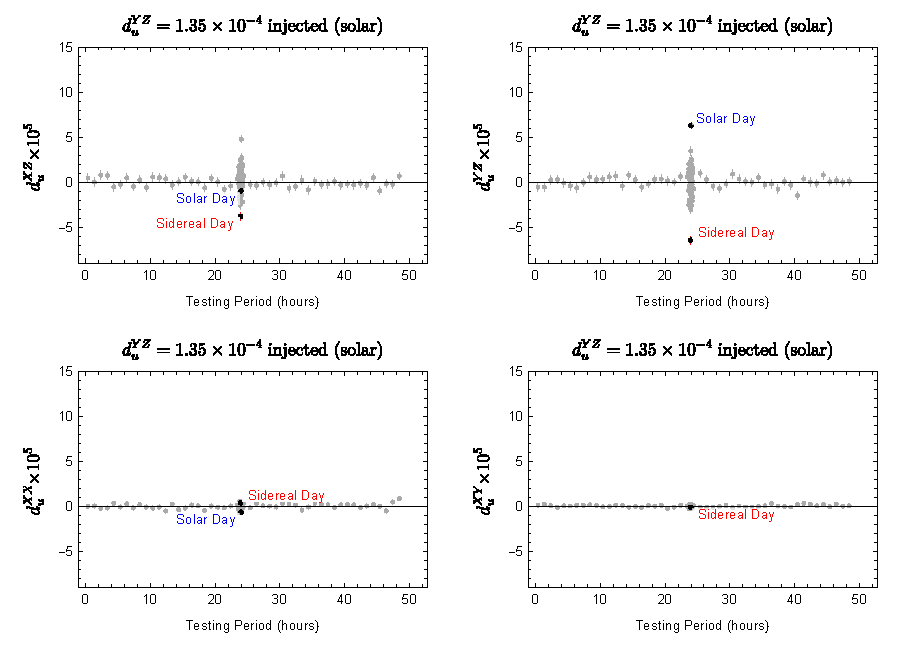
\includegraphics[width=0.8\textwidth]{figs/Mathematica-oldchi2/fit_duYZinjected_solar_scan-wide}
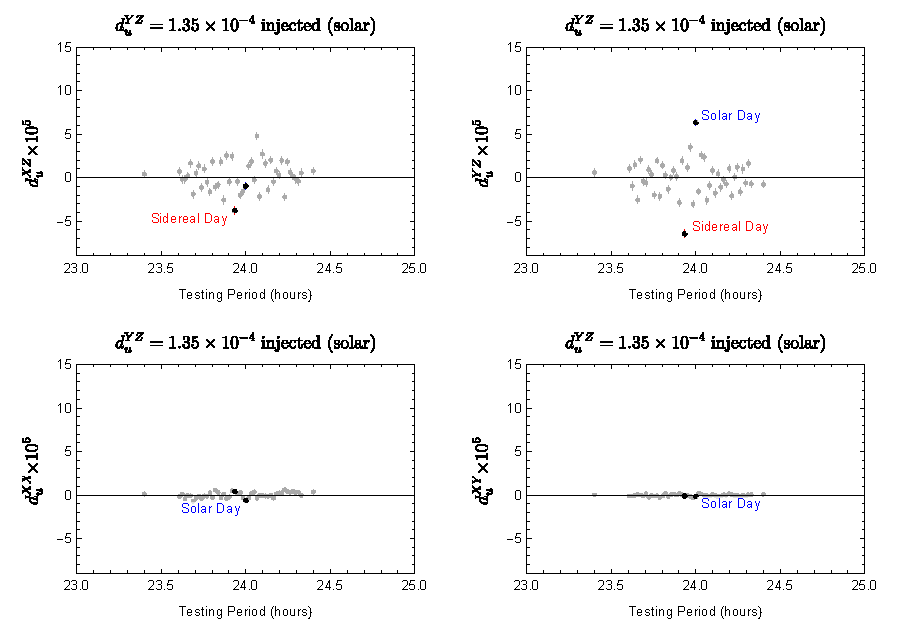
\includegraphics[width=0.8\textwidth]{figs/Mathematica-oldchi2/fit_duYZinjected_solar_scan-narrow}
\caption{Solar signal injection ($d_u^{YZ} = 1.35 \times 10^{-4}$). Fit for the $d_u^{YZ}$ coefficient as a function of the testing phase. Red and blue fits correspond to the sidereal and solar testing phases.}
\label{fig:RD_solar_signal_scan}
\end{figure}



\clearpage
\section{Double ratio simulation studies: multiple sampling}
\label{sec:double_ratio_multiple}
In this section we investigate whether there are intrinsic time structures which might bias the signal extraction. We do this by considering 1000 iterations of the various analyses presented in section~\ref{sec:double_ratio} and \ref{sec:double_ratio_injection_studies}.

In particular, we will:
\begin{enumerate}
    \item Study the distribution of the extracted coefficients in multiple SM samples to check whether they are centered around zero.
    \item Consider one sample which yields a 3 sigma deviation from zero for one coefficient (which is to be expected when looking at 1000 samples) and scramble its time stamps 1000 times. The purpose is to see whether some memory of the 3 sigma tension remains after scrambling.
    \item We generate one sample with a sidereal signal injection and scramble its time stamps 1000 times. This is a test for partial unblinding of the data.
    \item We generate 1000 injected samples (with the same coefficient) and study each one of them over a range of testing phases. We then look at the average of the extracted coefficient for each testing phase. This will produce a ``chirp'' structure (in the testing phase vs fitted coefficient plane). When looking at a given sample, the fitted coefficients will lie on a ``sampled'' version of this curve. 
\end{enumerate}

\subsection{SM simulation: multiple samples}
\label{ssec:SM_1000}
%
We repeated 1000 times the analysis presented in section~\ref{ssec:all_errors_included} with the purpose of checking whether the fitted coefficients are distributed around zero. This is indeed the case as can be seen in figure~\ref{fig:SM_1000}. In the figures we display both the average uncertainty of the fitted values ($\langle \delta d_u^{YZ} \rangle$) and the standard deviation of the central values ($\sigma ([d_u^{YZ}]_\text{CV})$). The (expected) agreement between the two signal a nice Gaussian distribution of the results. This agreement persists for all other coefficiences (not shown).

In figures~\ref{fig:SM_1000_fits_sidsol} and \ref{fig:SM_1000_fits_1h} we show the average and standard deviations for all fitted coefficients. We see that they are all strictly centered at zero.

\begin{figure}[H]
\centering
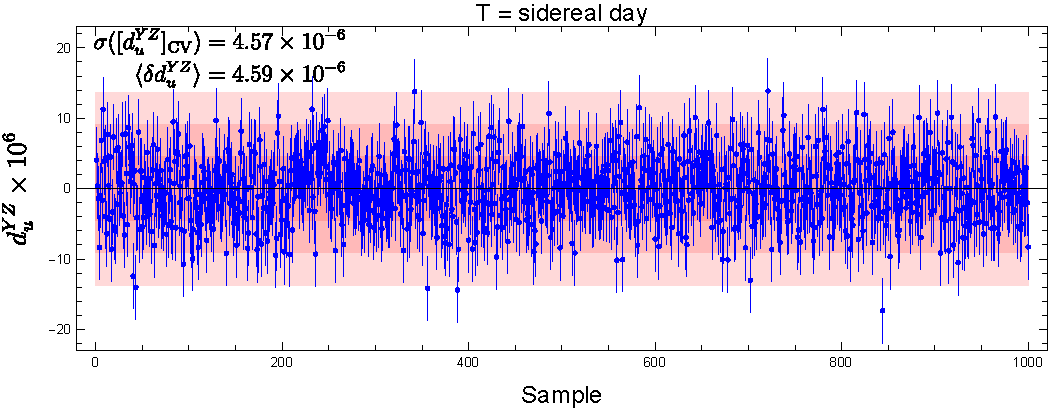
\includegraphics[width=\textwidth]{figs/Mathematica-oldchi2/fit_duYZ_SM_1000samples_sday}
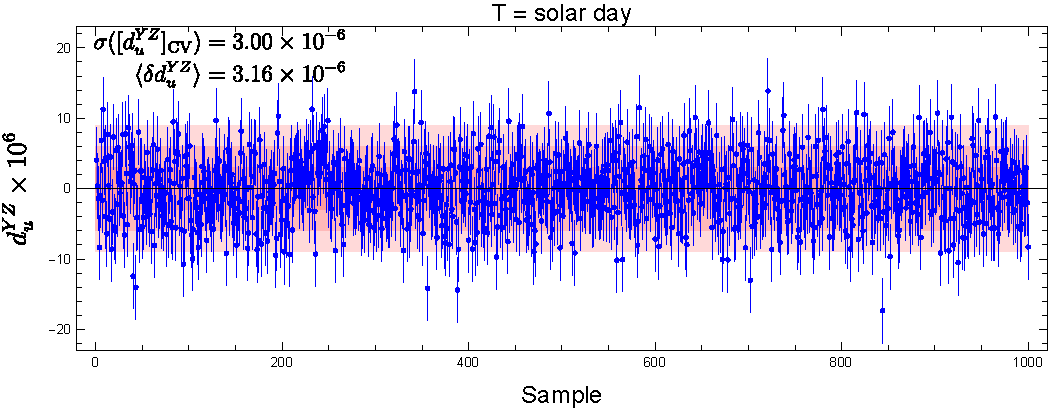
\includegraphics[width=\textwidth]{figs/Mathematica-oldchi2/fit_duYZ_SM_1000samples_day}
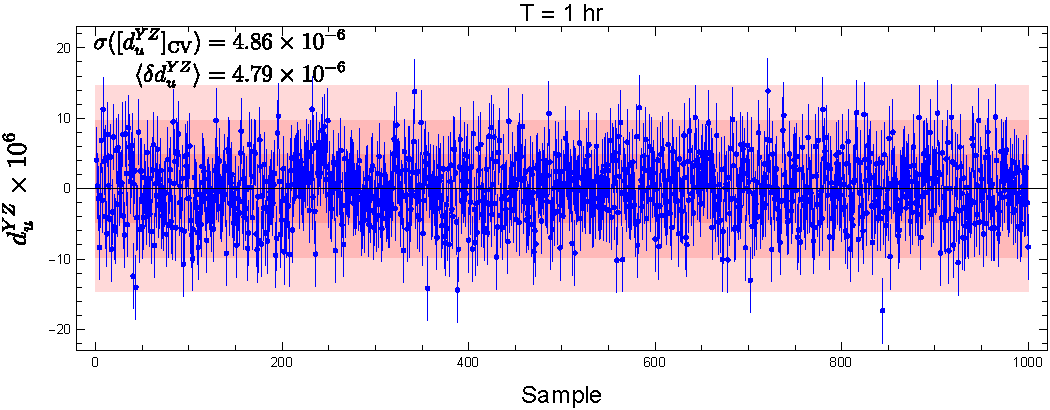
\includegraphics[width=\textwidth]{figs/Mathematica-oldchi2/fit_duYZ_SM_1000samples_1}
\caption{Distribution of the fitted coefficient $d_u^{YZ}$ extracted from 1000 SM samples. The three panels correspond to sidereal, solar and 1 hr testing phases. \textcolor{red}{The solar distribution seems too narrow. }}
\label{fig:SM_1000}
\end{figure} 


\begin{figure}[H]
\centering
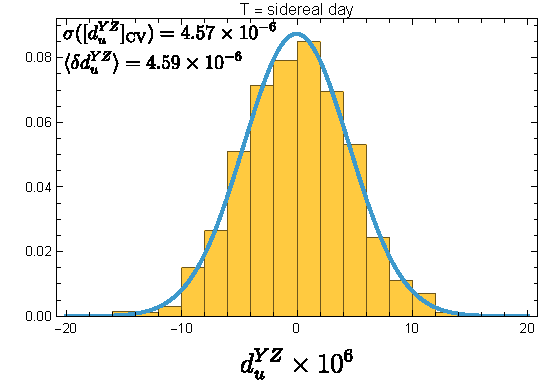
\includegraphics[width=.32\textwidth]{figs/Mathematica-oldchi2/fit_duYZ_SM_1000samples_sday_hist}
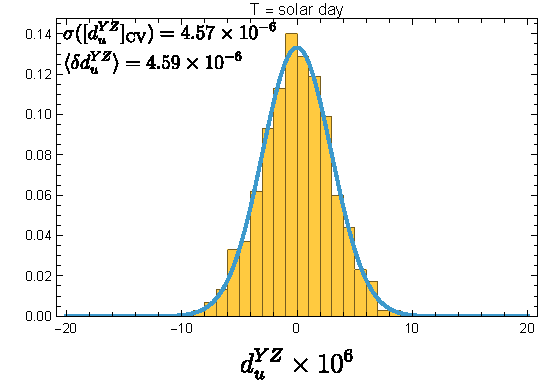
\includegraphics[width=.32\textwidth]{figs/Mathematica-oldchi2/fit_duYZ_SM_1000samples_day_hist}
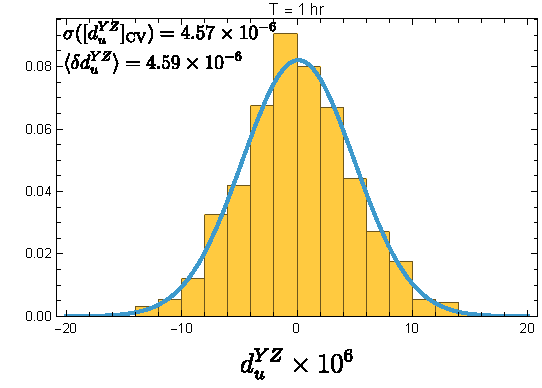
\includegraphics[width=.32\textwidth]{figs/Mathematica-oldchi2/fit_duYZ_SM_1000samples_1_hist}
\caption{Histogram of the distribution of the fitted coefficient $d_u^{YZ}$ extracted from 1000 SM samples. The three panels correspond to sidereal, solar and 1 hr testing phases. \textcolor{red}{The solar distribution seems too narrow. }}
\label{fig:SM_1000_hist}
\end{figure} 




\begin{figure}[H]
\centering
\begin{minipage}[H]{\textwidth}
    \vspace{0pt}
    \centering
   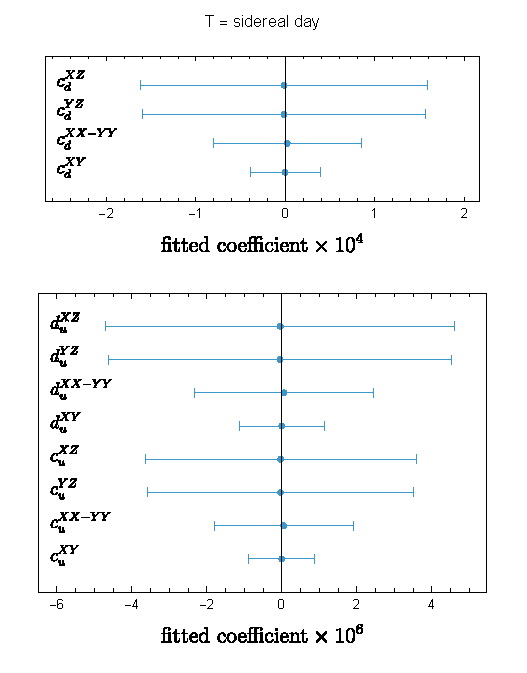
\includegraphics[width=0.49\textwidth]{figs/Mathematica-oldchi2/fit_duYZ_SM_1000samples_sday_fit}
   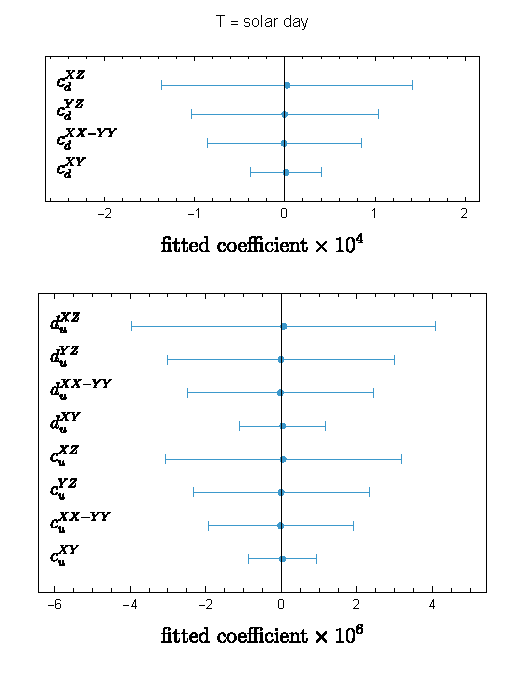
\includegraphics[width=0.49\textwidth]{figs/Mathematica-oldchi2/fit_duYZ_SM_1000samples_day_fit}
\end{minipage}
\begin{minipage}[H]{\textwidth}
    \vspace{1.6cm}
    \centering
    \begin{tabular}{|l|c|}
        \hline
$d_u^{XZ}$ & $(0. \pm 4.6)\times 10^{-6}$ \\
$d_u^{YZ}$ & $(-0. \pm 4.6)\times 10^{-6}$ \\
$d_u^{XX-YY}$ & $(0. \pm 2.4)\times 10^{-6}$ \\
$d_u^{XY}$ & $(0. \pm 11.)\times 10^{-7}$ \\
$c_u^{XZ}$ & $(0. \pm 3.6)\times 10^{-6}$ \\
$c_u^{YZ}$ & $(-0. \pm 3.5)\times 10^{-6}$ \\
$c_u^{XX-YY}$ & $(0. \pm 1.9)\times 10^{-6}$ \\
$c_u^{XY}$ & $(0. \pm 8.8)\times 10^{-7}$ \\
$c_d^{XZ}$ & $(0. \pm 1.6)\times 10^{-4}$ \\
$c_d^{YZ}$ & $(-0. \pm 1.6)\times 10^{-4}$ \\
$c_d^{XX-YY}$ & $(0.2 \pm 8.3)\times 10^{-5}$ \\
$c_d^{XY}$ & $(0. \pm 3.9)\times 10^{-5}$ \\
                \hline
        \end{tabular}
        \;\;\;\;\;\;\;\;\;\;\;\;\;\;\;\;\;\;
    \begin{tabular}{|l|c|}
        \hline
$d_u^{XZ}$ & $(0. \pm 4.0)\times 10^{-6}$ \\
$d_u^{YZ}$ & $(0. \pm 3.0)\times 10^{-6}$ \\
$d_u^{XX-YY}$ & $(-0. \pm 2.5)\times 10^{-6}$ \\
$d_u^{XY}$ & $(0. \pm 11.)\times 10^{-7}$ \\
$c_u^{XZ}$ & $(0. \pm 3.1)\times 10^{-6}$ \\
$c_u^{YZ}$ & $(0. \pm 2.3)\times 10^{-6}$ \\
$c_u^{XX-YY}$ & $(-0. \pm 1.9)\times 10^{-6}$ \\
$c_u^{XY}$ & $(0.3 \pm 8.9)\times 10^{-7}$ \\
$c_d^{XZ}$ & $(0. \pm 1.4)\times 10^{-4}$ \\
$c_d^{YZ}$ & $(0. \pm 1.0)\times 10^{-4}$ \\
$c_d^{XX-YY}$ & $(-0. \pm 8.5)\times 10^{-5}$ \\
$c_d^{XY}$ & $(0.1 \pm 3.9)\times 10^{-5}$ \\
                        \hline
        \end{tabular}
\end{minipage}
\caption{Sidereal signal injection test ($d_u^{YZ} = 1.35 \times 10^{-4}$): fit results for sidereal (left) and solar (right) testing phases.}
\label{fig:SM_1000_fits_sidsol}
\end{figure}


\begin{figure}[H]
\centering
\begin{minipage}[H]{0.49\textwidth}
    \vspace{1.6cm}
    \centering
    \begin{tabular}{|l|c|}
        \hline
$d_u^{XZ}$ & $(0.3 \pm 4.9)\times 10^{-6}$ \\
$d_u^{YZ}$ & $(0.1 \pm 4.9)\times 10^{-6}$ \\
$d_u^{XX-YY}$ & $(-0. \pm 2.4)\times 10^{-6}$ \\
$d_u^{XY}$ & $(0. \pm 12.)\times 10^{-7}$ \\
$c_u^{XZ}$ & $(0.2 \pm 3.8)\times 10^{-6}$ \\
$c_u^{YZ}$ & $(0. \pm 3.8)\times 10^{-6}$ \\
$c_u^{XX-YY}$ & $(-0. \pm 1.9)\times 10^{-6}$ \\
$c_u^{XY}$ & $(0.3 \pm 9.6)\times 10^{-7}$ \\
$c_d^{XZ}$ & $(0. \pm 1.7)\times 10^{-4}$ \\
$c_d^{YZ}$ & $(0. \pm 1.7)\times 10^{-4}$ \\
$c_d^{XX-YY}$ & $(-0.1 \pm 8.3)\times 10^{-5}$ \\
$c_d^{XY}$ & $(0.1 \pm 4.3)\times 10^{-5}$ \\
        \hline
        \end{tabular}
\end{minipage}
\begin{minipage}[H]{0.49\textwidth}
    \vspace{0pt}
    \centering
   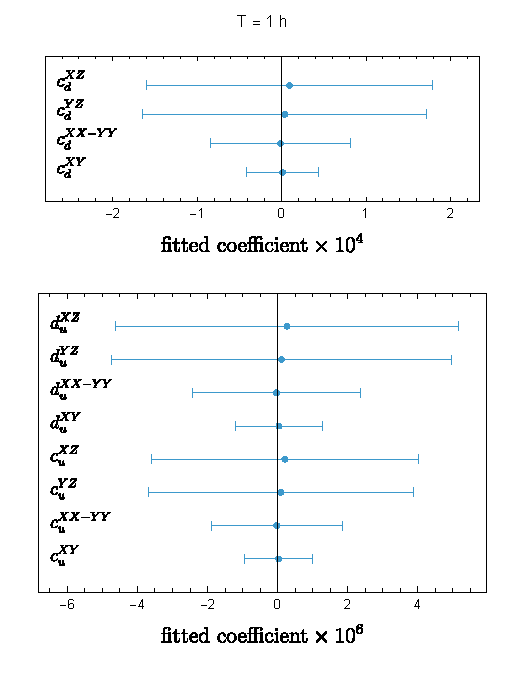
\includegraphics[width=\textwidth]{figs/Mathematica-oldchi2/fit_duYZ_SM_1000samples_1_fit}
\end{minipage}
\caption{Sidereal signal injection test ($d_u^{YZ} = 1.35 \times 10^{-4}$): fit results for 1 hr testing phase.}
\label{fig:SM_1000_fits_1h}
\end{figure}


\subsection{Multiple time scramblings of ``bad'' sample}
\label{ssec:bad_sample}
%
In this section we select one of the samples we generated in section~\ref{ssec:SM_1000} for a which the fitted value of a coefficient deviates from zero at the three sigma level. Sample \#844 yields a $3.8\;\sigma$ tension: $\left[d_u^{YZ}\right]_\text{fit} = -(1.73 \pm 0.46) \times 10^{-5}$. Note that this is not an anomaly but simply a statistical necessity given the number of the generated samples. The question is whether multiple scramblings of this sample will retain a memory of this tension. The result of this study is presented in figure~\ref{fig:SM_1000_bad_sample}, from which we see that no memory of the initial tension remains in the 1000 successive scramblings. 

\begin{figure}[H]
\centering
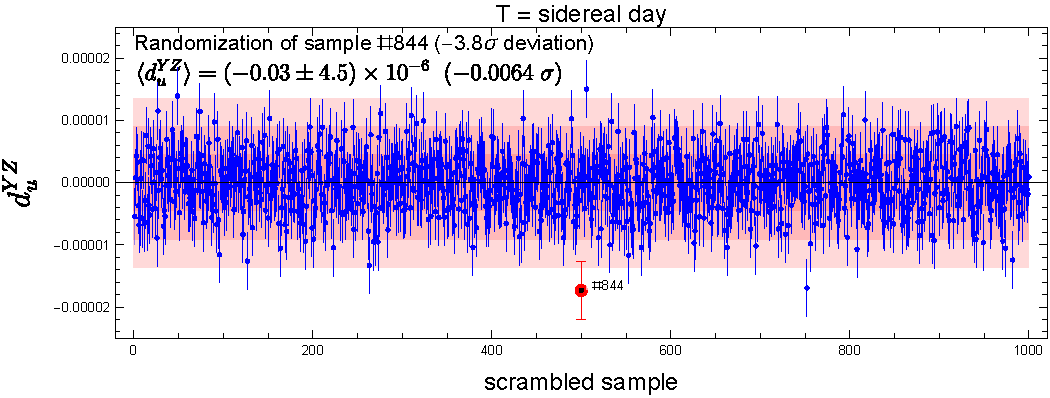
\includegraphics[width=\textwidth]{figs/Mathematica-oldchi2/fit_duYZ_SM_sample844_1000scrambles}
\caption{1000 scramblings of sample \#844 which displays an accidental 3.8 sigma tension.}
\label{fig:SM_1000_bad_sample}
\end{figure}


\subsection{Multiple time scramblings of an injected signal}
\label{ssec:signal_1000scramblings}
%
In this test, we inject a $d_u^{YZ} = 1.35 \times 10^{-4}$ signal. Typically this signal will yield results like those presented in section~\ref{ssec:SiderealInjectionRecovery} (figures~\ref{fig:RD_sidereal_signal} and \ref{fig:RD_sidereal_signal_fits_sidsol}). Here we consider 1000 scrambles of the time stamps of this sample and perform a sidereal time analysis. The purpose of this is to show that no memory of the signal remains. The result of this study is presented in figure~\ref{fig:sidereal_signal_1000_scrambles}.

\begin{figure}[H]
\centering
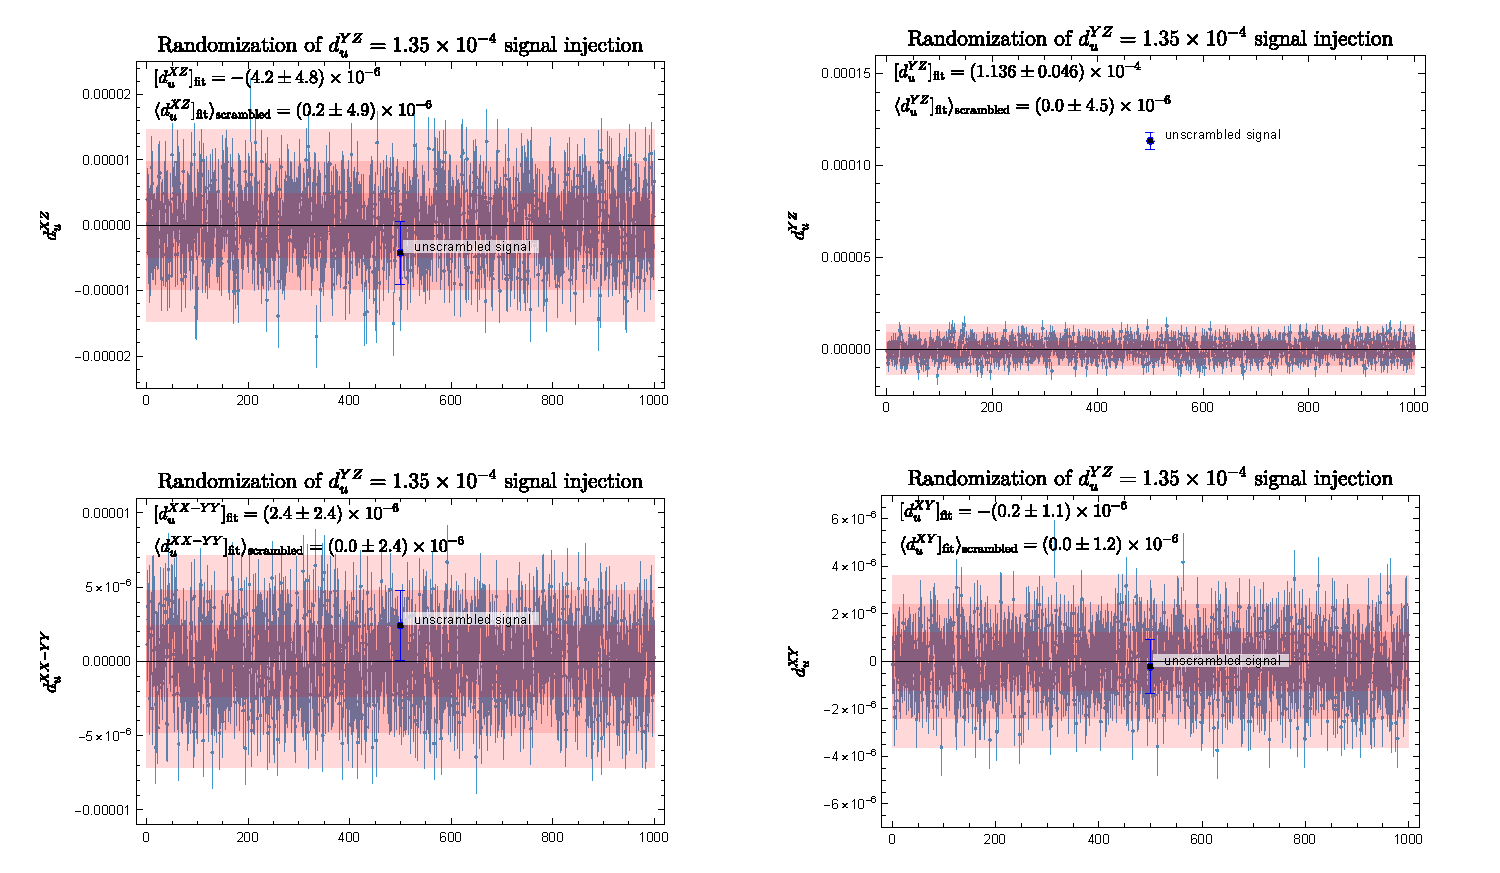
\includegraphics[width=\textwidth]{figs/Mathematica-oldchi2/fit_duYZinjected_1000scrambles}
\caption{Distribution of the fitted coefficient $d_u^{YZ}$ obtained by scrambling 1000 times the time stamps of an injected signal. }
\label{fig:sidereal_signal_1000_scrambles}
\end{figure}


\subsection{Multiple samples of an injected signal analyzed over a range of testing phases}
\label{ssec:signal_1000samples_phasesscan}
%
In this section, we inject a $d_u^{YZ} = 1.35 \times 10^{-4}$ signal and generate 1000 samples. Each sample is than analyzed over a range of testing phases. For each testing phase we then average the 1000 fit outcomes. The results of this analysis are presented in figures~\ref{fig:sidereal_signal_1000_scrambles_scan_wide} and \ref{fig:sidereal_signal_1000_scrambles_scan_narrow}. The results we obtain for the sidereal, solar and 1 hr testing phases are summarized in figure~\ref{fig:sidereal_signal_1000_scrambles_scan_fit}. The ``chirp'' structures that we observe in figure~\ref{fig:sidereal_signal_1000_scrambles_scan_narrow} are not affected by the Poisson/Gaussian sampling and are a reflection of the intrinsic time structure of the data. 

\begin{figure}[H]
\centering
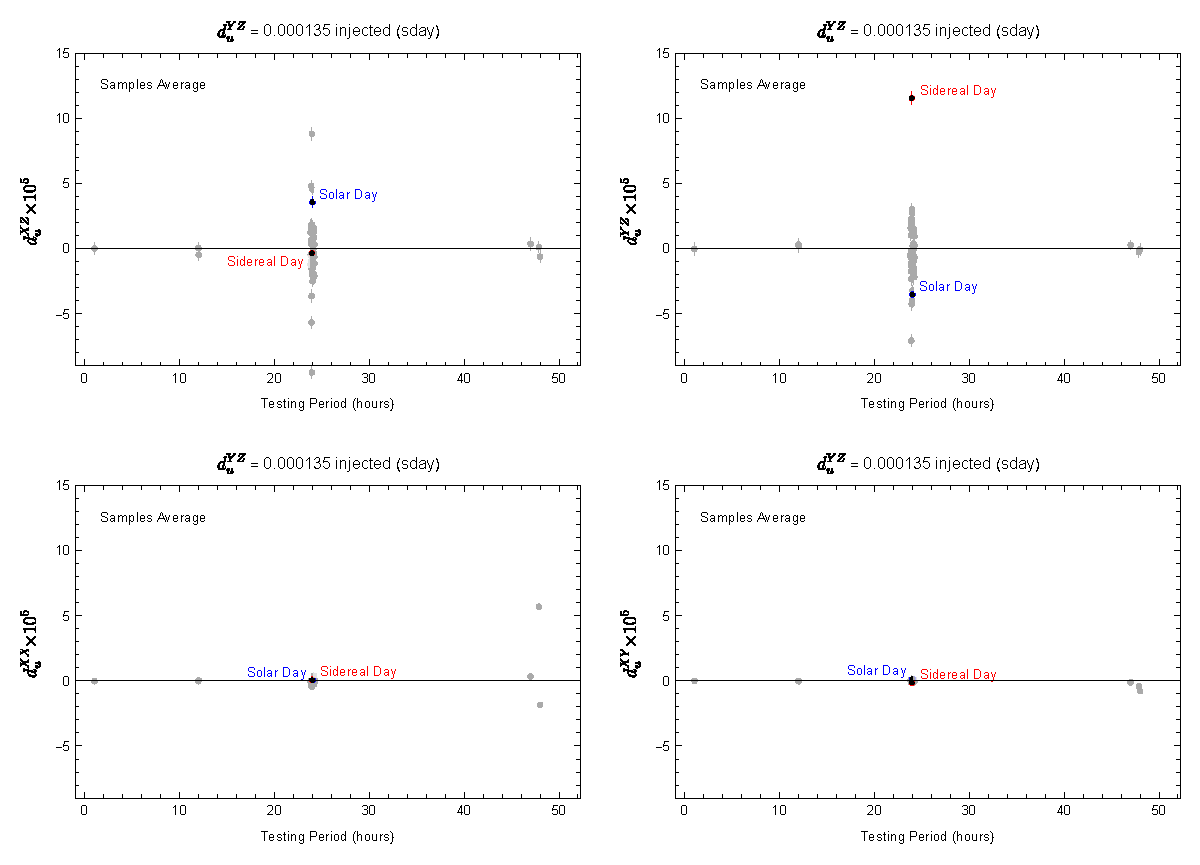
\includegraphics[width=\textwidth]{figs/Mathematica-oldchi2/fit_duYZinjected_1000samples_phasescan_wide}
\caption{Averages (over 1000 injections of a $d_u^{YZ} = 1.35 \times 10^{-4}$ sidereal signal) of the fit results for various SME coefficients as a function of the testing phase.}
\label{fig:sidereal_signal_1000_scrambles_scan_wide}
\end{figure}

\begin{figure}[H]
\centering
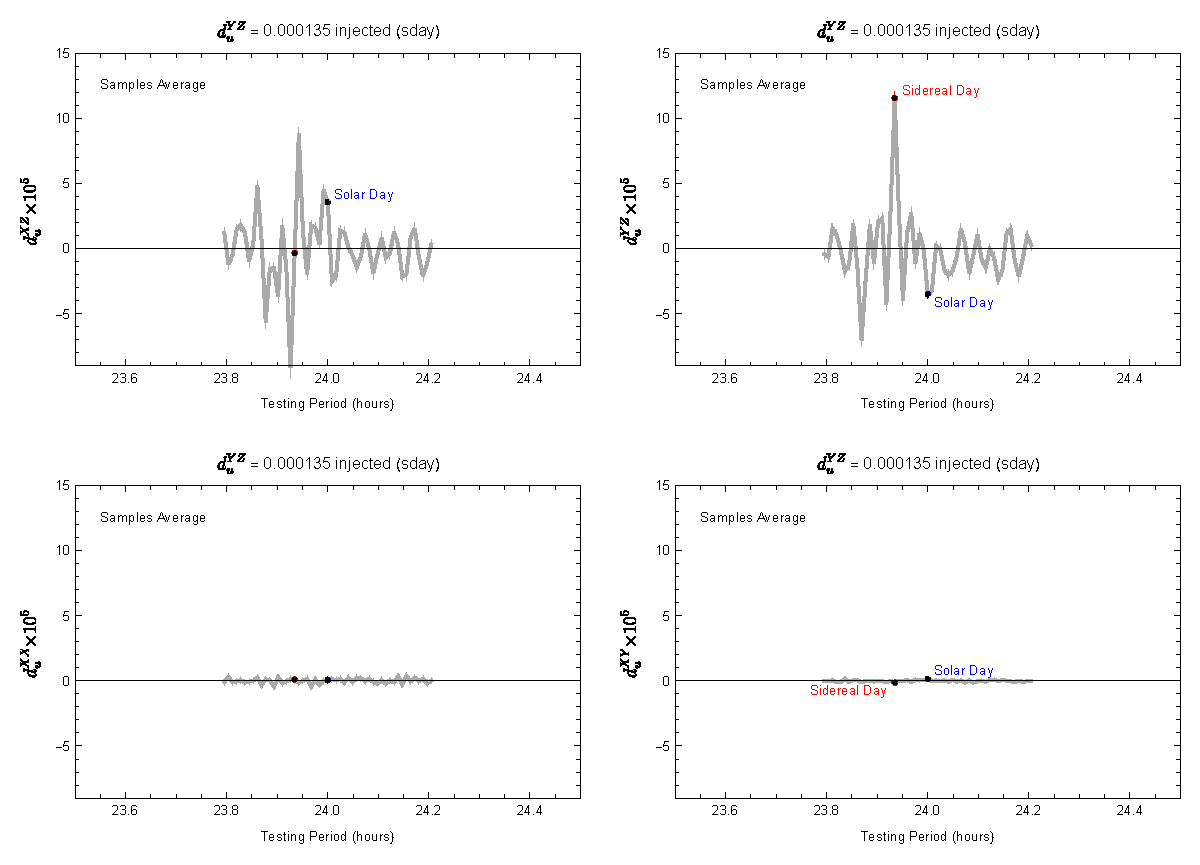
\includegraphics[width=\textwidth]{figs/Mathematica-oldchi2/fit_duYZinjected_1000samples_phasescan_narrow}
\caption{Averages (over 1000 injections of a $d_u^{YZ} = 1.35 \times 10^{-4}$ sidereal signal) of the fit results for various SME coefficients as a function of the testing phase (zoom).}
\label{fig:sidereal_signal_1000_scrambles_scan_narrow}
\end{figure}



\begin{figure}[H]
\centering
\begin{minipage}[H]{0.49\textwidth}
    \vspace{0pt}
    \centering
   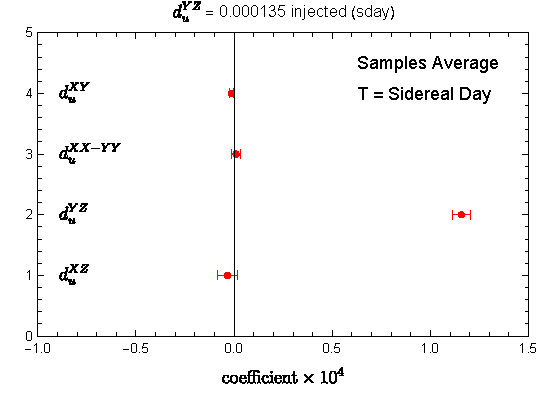
\includegraphics[width=\textwidth]{figs/Mathematica-oldchi2/fit_duYZinjected_1000samples_averages_sday}
\end{minipage}
\begin{minipage}[H]{0.49\textwidth}
    \vspace{0pt}
    \centering
 \begin{tabular}{|l|c|}
        \hline
        $d_u^{XY}$ & $ (-1.4 \pm 1.1)\times 10^{-6}$ \\
        $d_u^{XX-YY}$ & $ (1. \pm 2.3)\times 10^{-6}$ \\
        $d_u^{YZ}$ & $ (1.158 \pm 0.047)\times 10^{-4}$ \\
        $d_u^{XZ}$ & $ (-3.4 \pm 5.0)\times 10^{-6}$ \\
        \hline
    \end{tabular}
\end{minipage}
\begin{minipage}[H]{0.49\textwidth}
    \vspace{0pt}
    \centering
   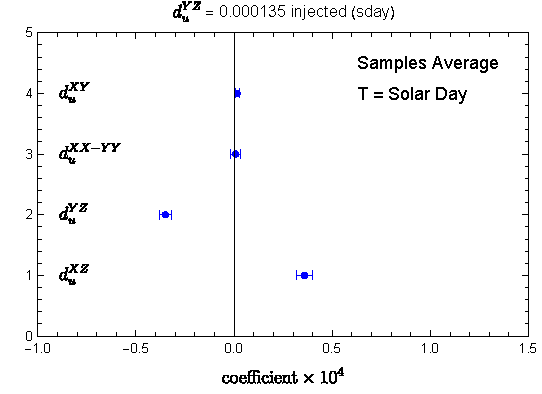
\includegraphics[width=\textwidth]{figs/Mathematica-oldchi2/fit_duYZinjected_1000samples_averages_day}
\end{minipage}
\begin{minipage}[H]{0.49\textwidth}
    \vspace{0pt}
    \centering
    \begin{tabular}{|l|c|}
        \hline
        $d_u^{XY}$ & $ (1.6 \pm 1.1)\times 10^{-6}$ \\
        $d_u^{XX-YY}$ & $ (0.7 \pm 2.4)\times 10^{-6}$ \\
        $d_u^{YZ}$ & $ (-3.50 \pm 0.32)\times 10^{-5}$ \\
        $d_u^{XZ}$ & $ (3.6 \pm 0.40)\times 10^{-5}$ \\
        \hline
        \end{tabular}
\end{minipage}
\begin{minipage}[H]{0.49\textwidth}
    \vspace{0pt}
    \centering
   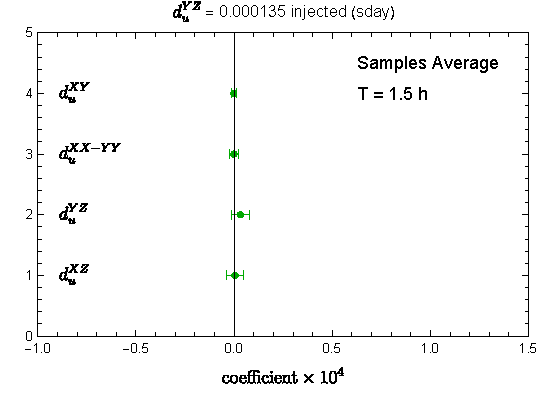
\includegraphics[width=\textwidth]{figs/Mathematica-oldchi2/fit_duYZinjected_1000samples_averages_1.5}
\end{minipage}
\begin{minipage}[H]{0.49\textwidth}
    \vspace{0pt}
    \centering
    \begin{tabular}{|l|c|}
        \hline
        $d_u^{XY}$ & $ (0.03 \pm 1.2)\times 10^{-6}$ \\
        $d_u^{XX-YY}$ & $ (-0.2 \pm 2.4)\times 10^{-6}$ \\
        $d_u^{YZ}$ & $ (-0.2 \pm 4.7)\times 10^{-6}$ \\
        $d_u^{XZ}$ & $ (0.1 \pm 4.8)\times 10^{-6}$ \\
        \hline
        \end{tabular}
\end{minipage}
\caption{Sidereal signal injection test ($d_u^{YZ} = 1.35 \times 10^{-4}$): fit results for sidereal (left) and solar (right) testing phases.}
\label{fig:sidereal_signal_1000_scrambles_scan_fit}
\end{figure}




\clearpage
\section{To do}
\begin{itemize}
    \item Varying the number of bins.
    \item Investigate different options to assign a unique time stamp to LBs. Options are: (1) Using $t_\text{initial}$ or $t_\text{final}$ rather than the average; (2) Use a random time in the $[t_\text{initial},t_\text{final}]$ range; (3) Investigate whether it makes sense to split LBs if the $[t_\text{initial},t_\text{final}]$ range straddles two time bins.
    \item Scrambling of 15 mins bins.
    \item Do an unbinned study using the Lomb-Scargle approach.
    \item Add constraints on $c_s^{AB}$, $d_s^{AB}$ and $a^{(5)ABC}$ coefficients.
\end{itemize}

\clearpage
\section{Luminosity-data driven toy studies}  %% [Yuji]
\label{lab:ToyStudy}
%%% 4 Luminosity-data driven toy studies %% [Yuji]   

Main purpose of TOY study is to check basic principles of the measurement. 
This toy study is used for understanding of binning and sidereal phase, and estimating sensitivity also evaluate effect of systematic uncertainties. 

In this section, basics of our TOY model is described and show several studies with changing conditions. 

\subsection{Basic TOY model}
\label{sec:basic_TOYmodel}
One of most important target of this TOY study is to find any structure or non-uniformity in the double ratio as function of the sidereal phase. 
Because physics runs were taken when LHC was ready and setup, therefore the distribution of the time stamp of LBs is not uniform.
A time stamp depends on starting time of a run which depends on LHC beam condition and life time and ATLAS detector status. Also, instatenous luminosity is not uniform. 
It's not simple to simulate this time structure, therefore we use the actual time stamp of Run-2 data for this toy studies.
Fig.~\ref{fig:toy_lumiProfile} (left) shows the time profile of LBs of full Run-2 data, and their duration are plotted in Fig.~\ref{fig:toy_lumiProfile} (right).

\begin{figure}[b]
\centering
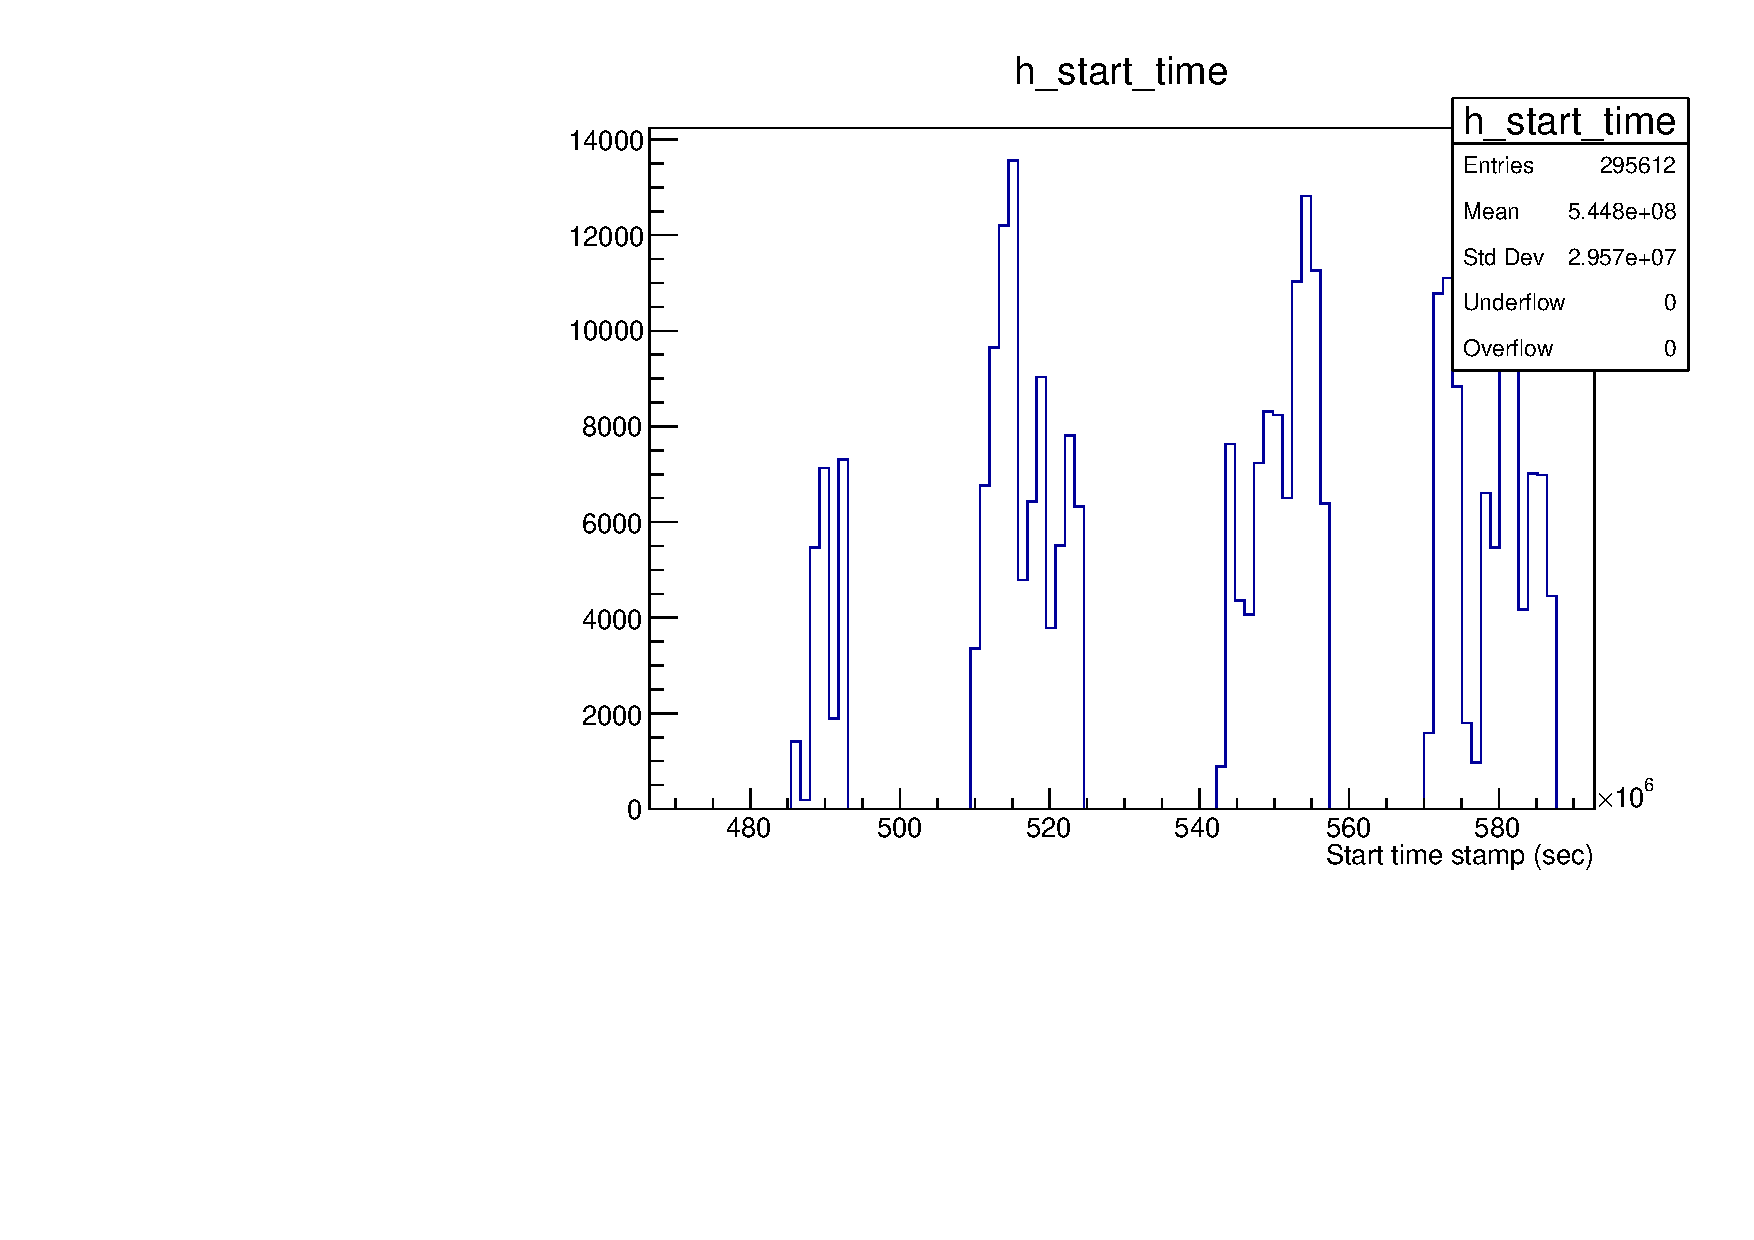
\includegraphics[width=0.4\textwidth]{figs/toy/fig_bin100_LIVxsec_0_random1_period1000_probe24_SigConfig0_LumiProf0_h_start_time.pdf}
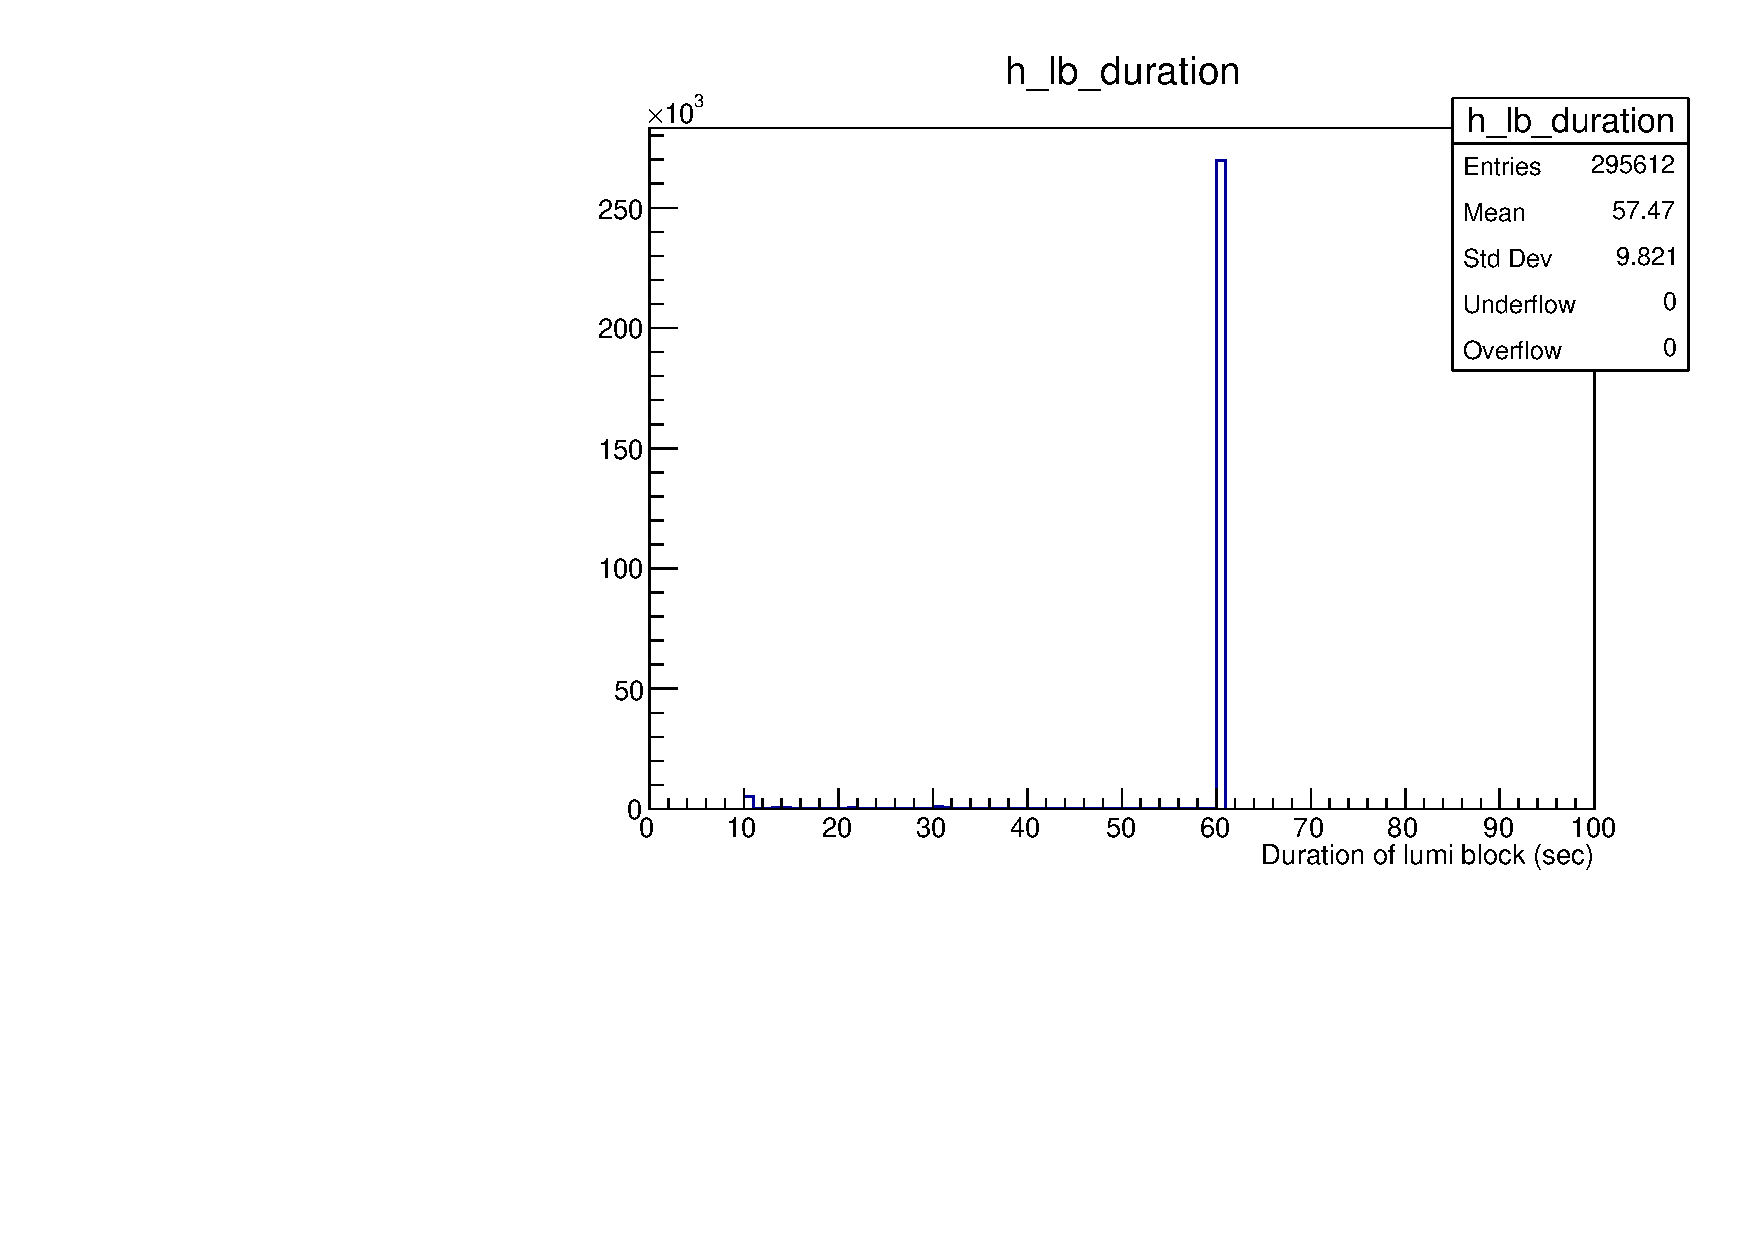
\includegraphics[width=0.4\textwidth]{figs/toy/fig_bin100_LIVxsec_0_random1_period1000_probe24_SigConfig0_LumiProf0_h_lb_duration.pdf}
\caption{\label{fig:toy_lumiProfile} Distribution of the time stamps of each Lumi block (left) and their duration (right). }
\end{figure}

As a basic TOY sample, the number of Z is computed each LB according to its duration and compute the Sidereal phase with following condition 
using only the time stamp of Lumi Block, and not use of other information in the actual data:
\begin{enumerate}
 \item use actual time stamp of each LB of Run-2 data.
 \item a Z fiducial cross sectin of 750 pb. (and inject LIV effect as function of sidereal phase if necessary)
 \item a flat instanteous luminosity of $1.0 \times 10^{34} cm^{-2} s^{-1}$ (as a simplest case). 
 \item introduce random effect on the computed number of Z by applying poisson statistics in each LB. 
 \item Siderial period, $T$, is 23h 56m 04s ($\sim$ 365 / 366 days). 
 \item $T_0$ is set March 20th 11:35 UTC, which is $T_0$ of SCF at the center of the ATLAS detector. (See Section~\ref{lab:Theory}).
\end{enumerate}

Histogram of number of LBs as function of the generated Sidereal period and sidereal phase are shown in Fig.~\ref{fig:toy_lb_period}.
These distributions are not flat because of run time (ATLAS is taking data when LHC makes collision when ATLAS detector is ready.) 
Distribution of the integrated luminosity as a function of sidereal phase and number of Z boson are shown in Fig.~\ref{fig:toy_numZ_phase}. 
Non-uniform structure of this distribution is due to the non-uniform profile of time stamp of the lumi blocks.
For example, a fill in 2018 started at 8:00 and lasted 7 hours and no other fill on the same day. In this case, 
we have measured the number of Z only 7 hours over 24 hours. 

\begin{figure}
\centering
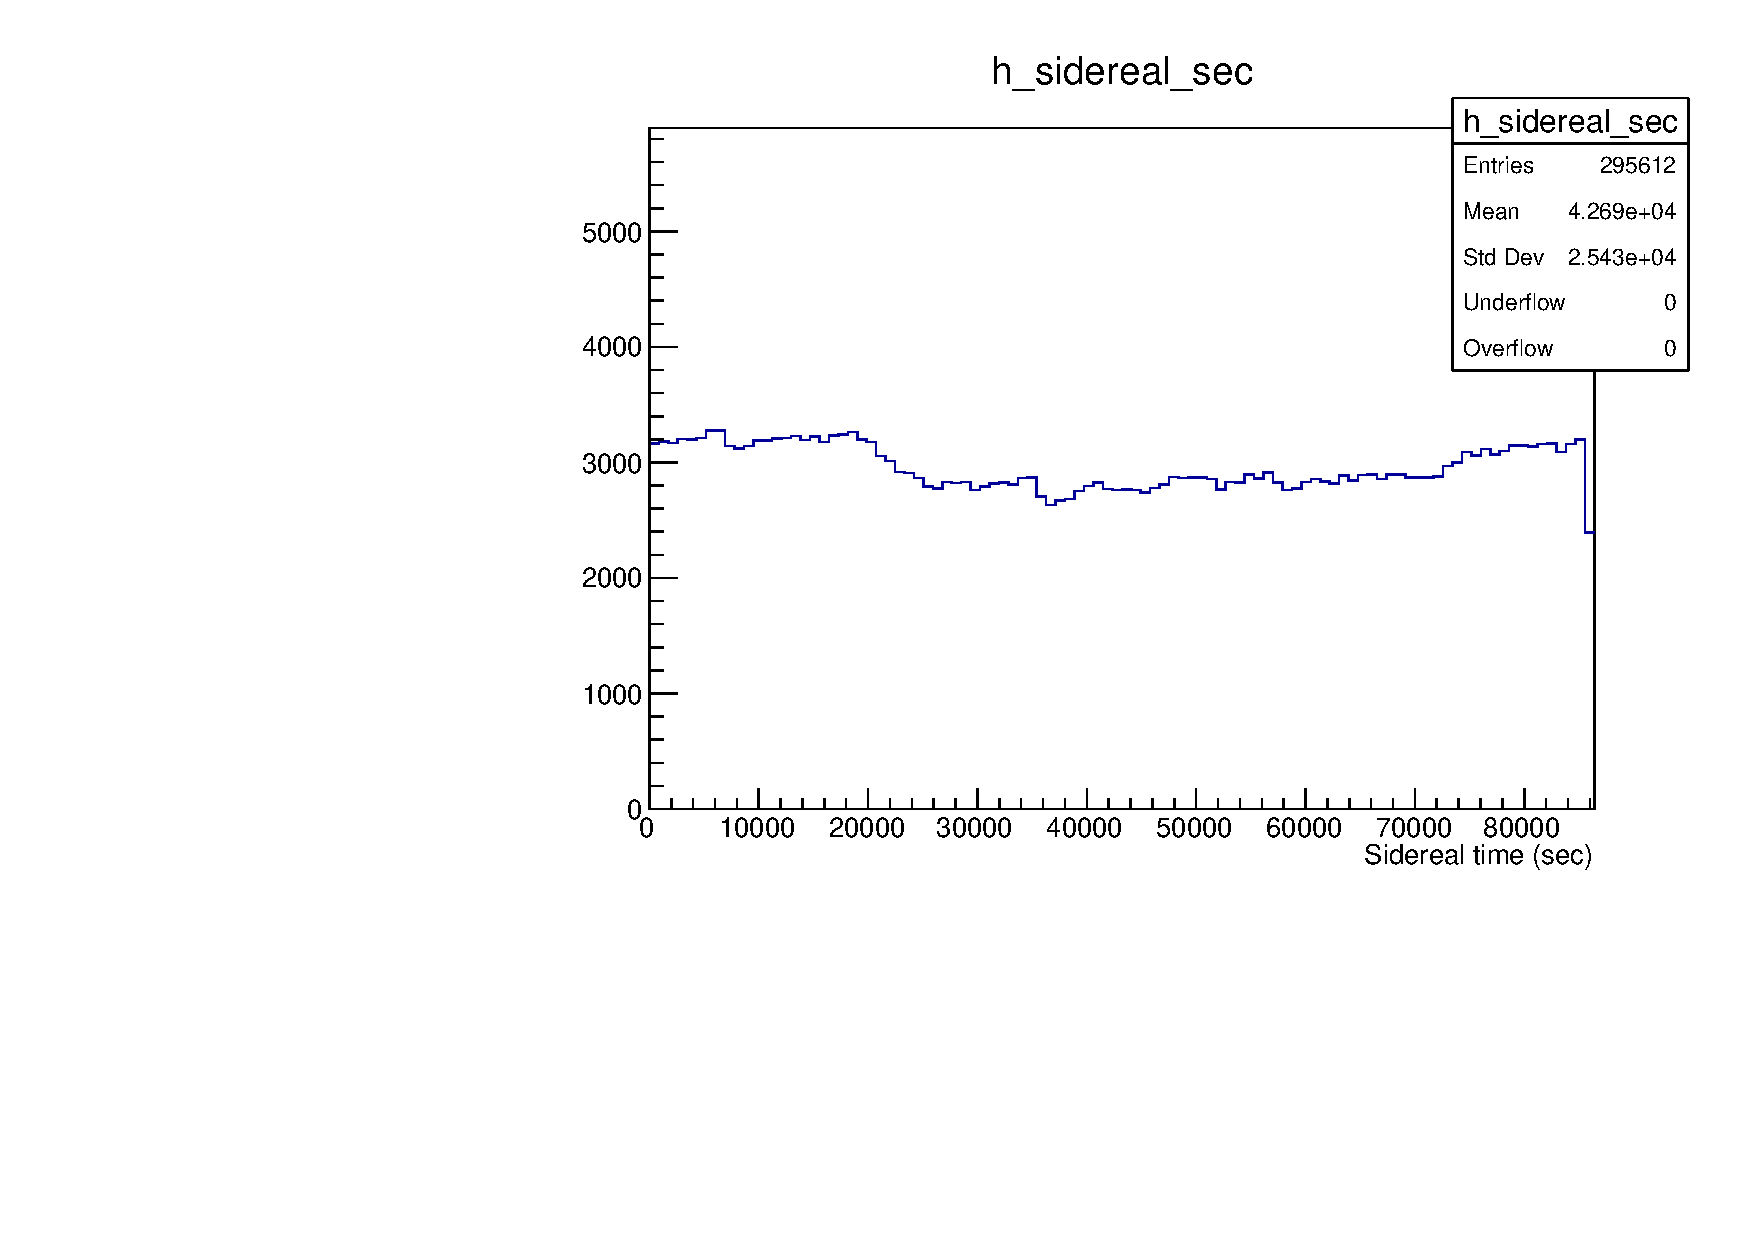
\includegraphics[width=0.4\textwidth]{figs/toy/fig_bin100_LIVxsec_0_random1_period1000_probe24_SigConfig0_LumiProf0_h_sidereal_sec.pdf}
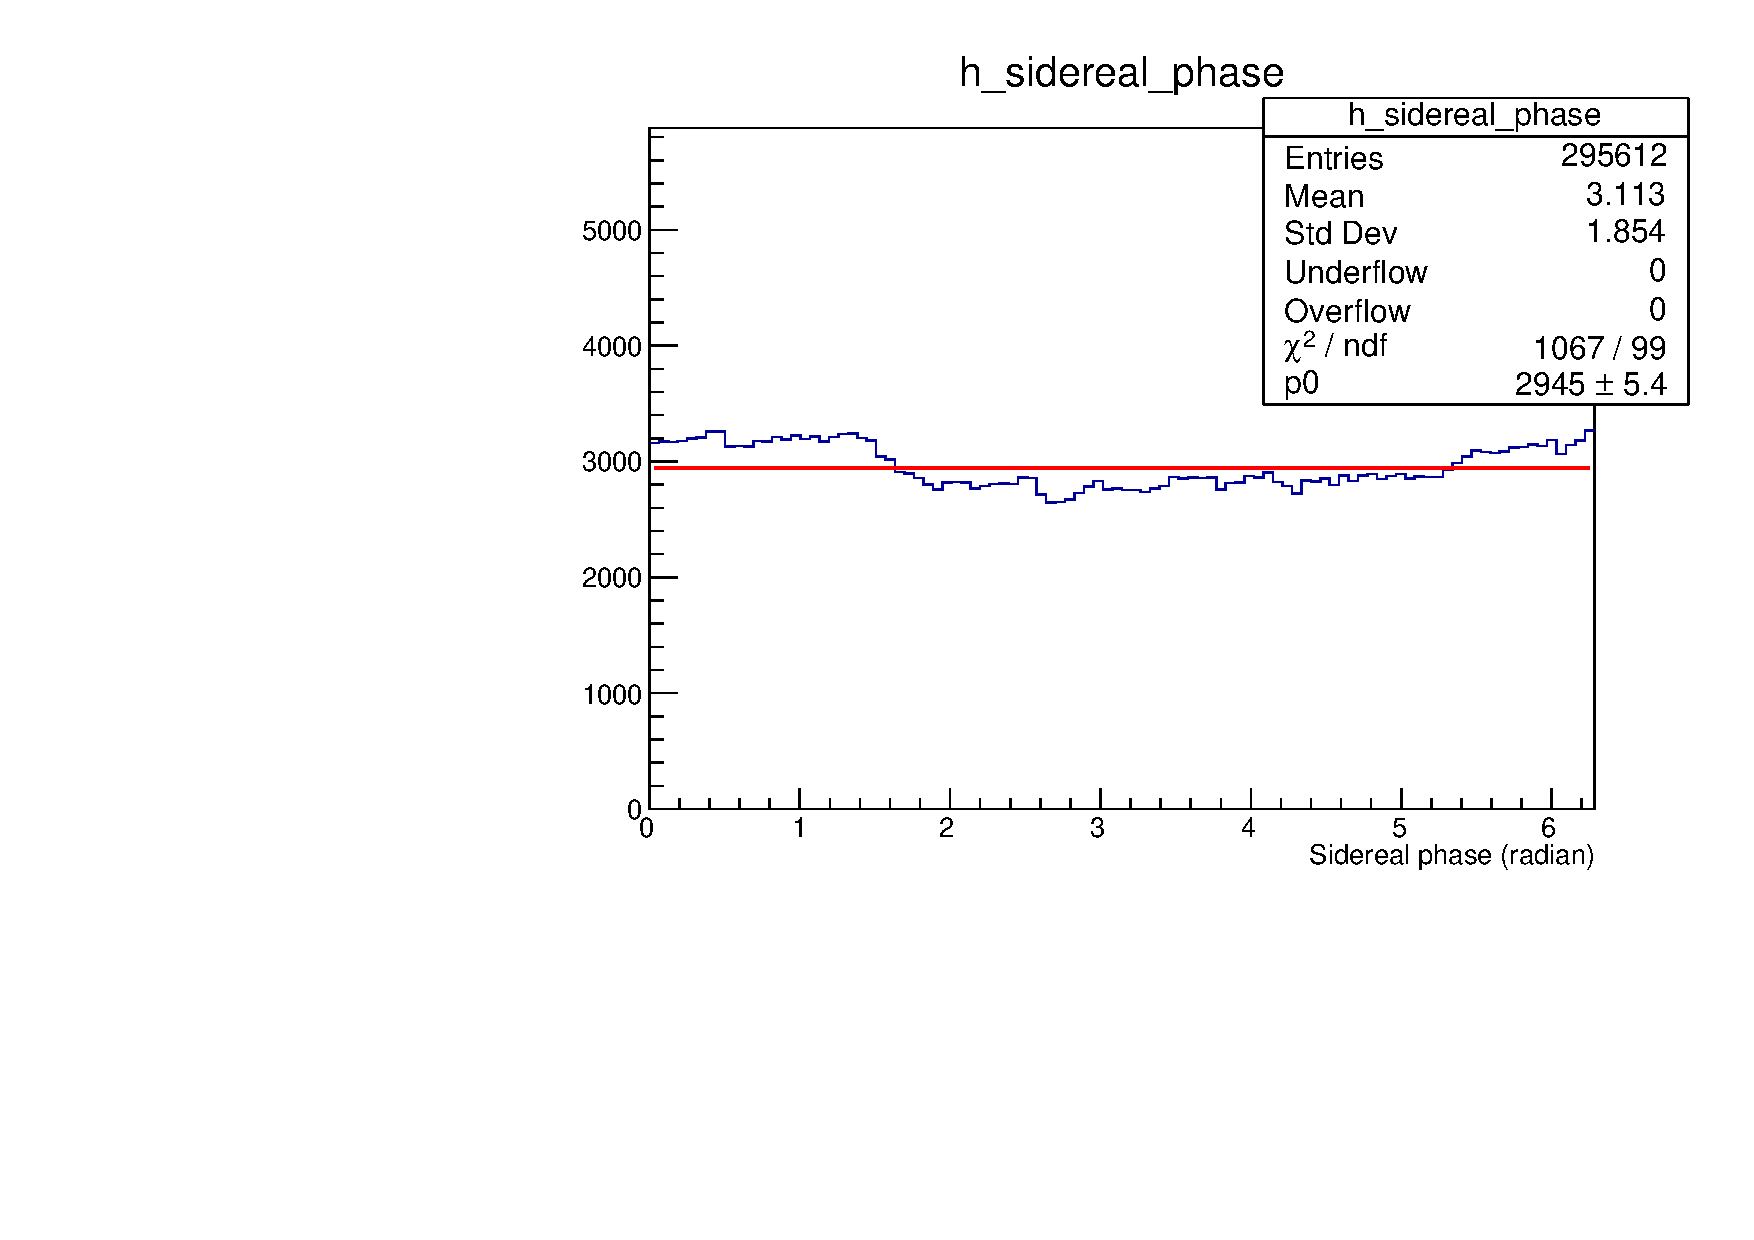
\includegraphics[width=0.4\textwidth]{figs/toy/fig_bin100_LIVxsec_0_random1_period1000_probe24_SigConfig0_LumiProf0_h_sidereal_phase.pdf}
\caption{\label{fig:toy_lb_period} Distribution of Lumi block as function of the sidereal period (left) and the sidereal phase (right). }
\end{figure}

\begin{figure}
\centering
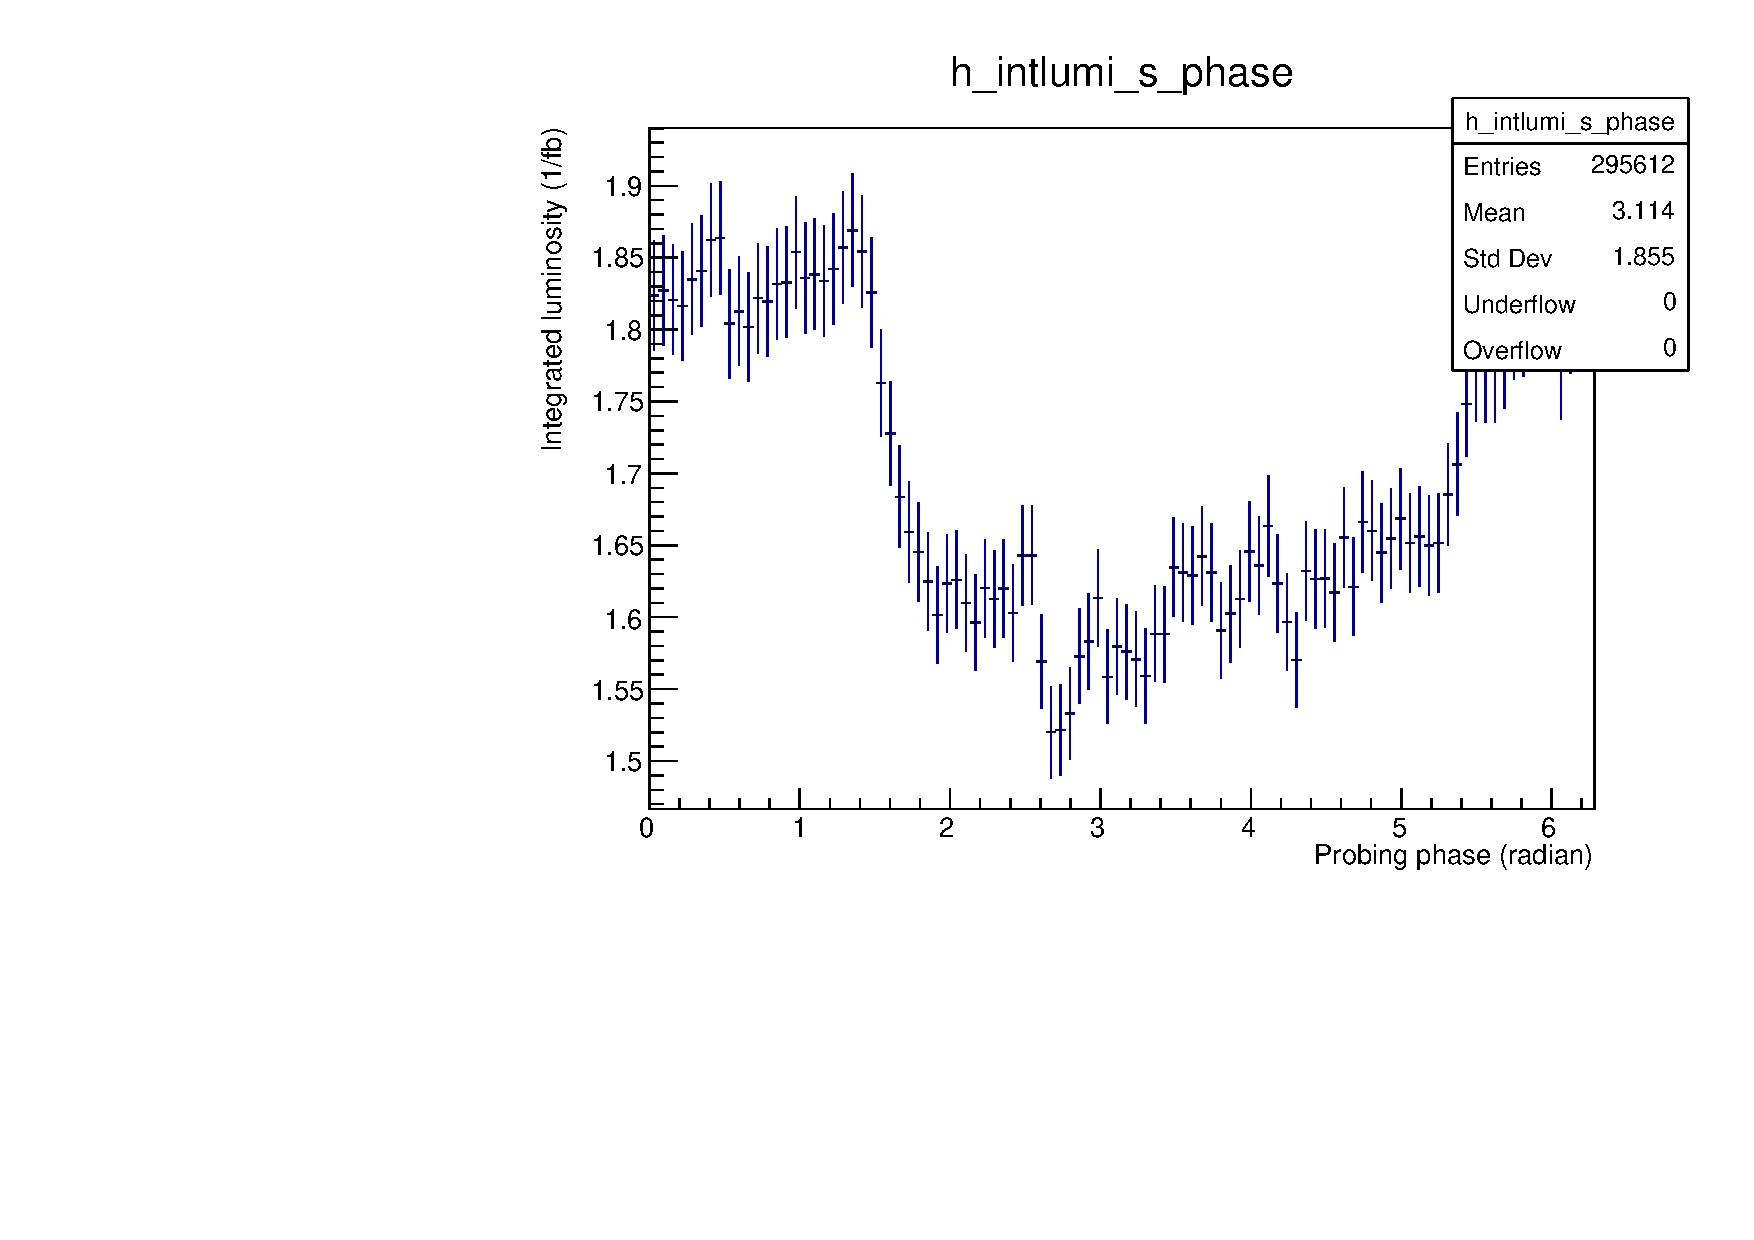
\includegraphics[width=0.4\textwidth]{figs/toy/fig_bin100_LIVxsec_0_random1_period1000_probe24_SigConfig0_LumiProf0_h_intlumi_s_phase.pdf}
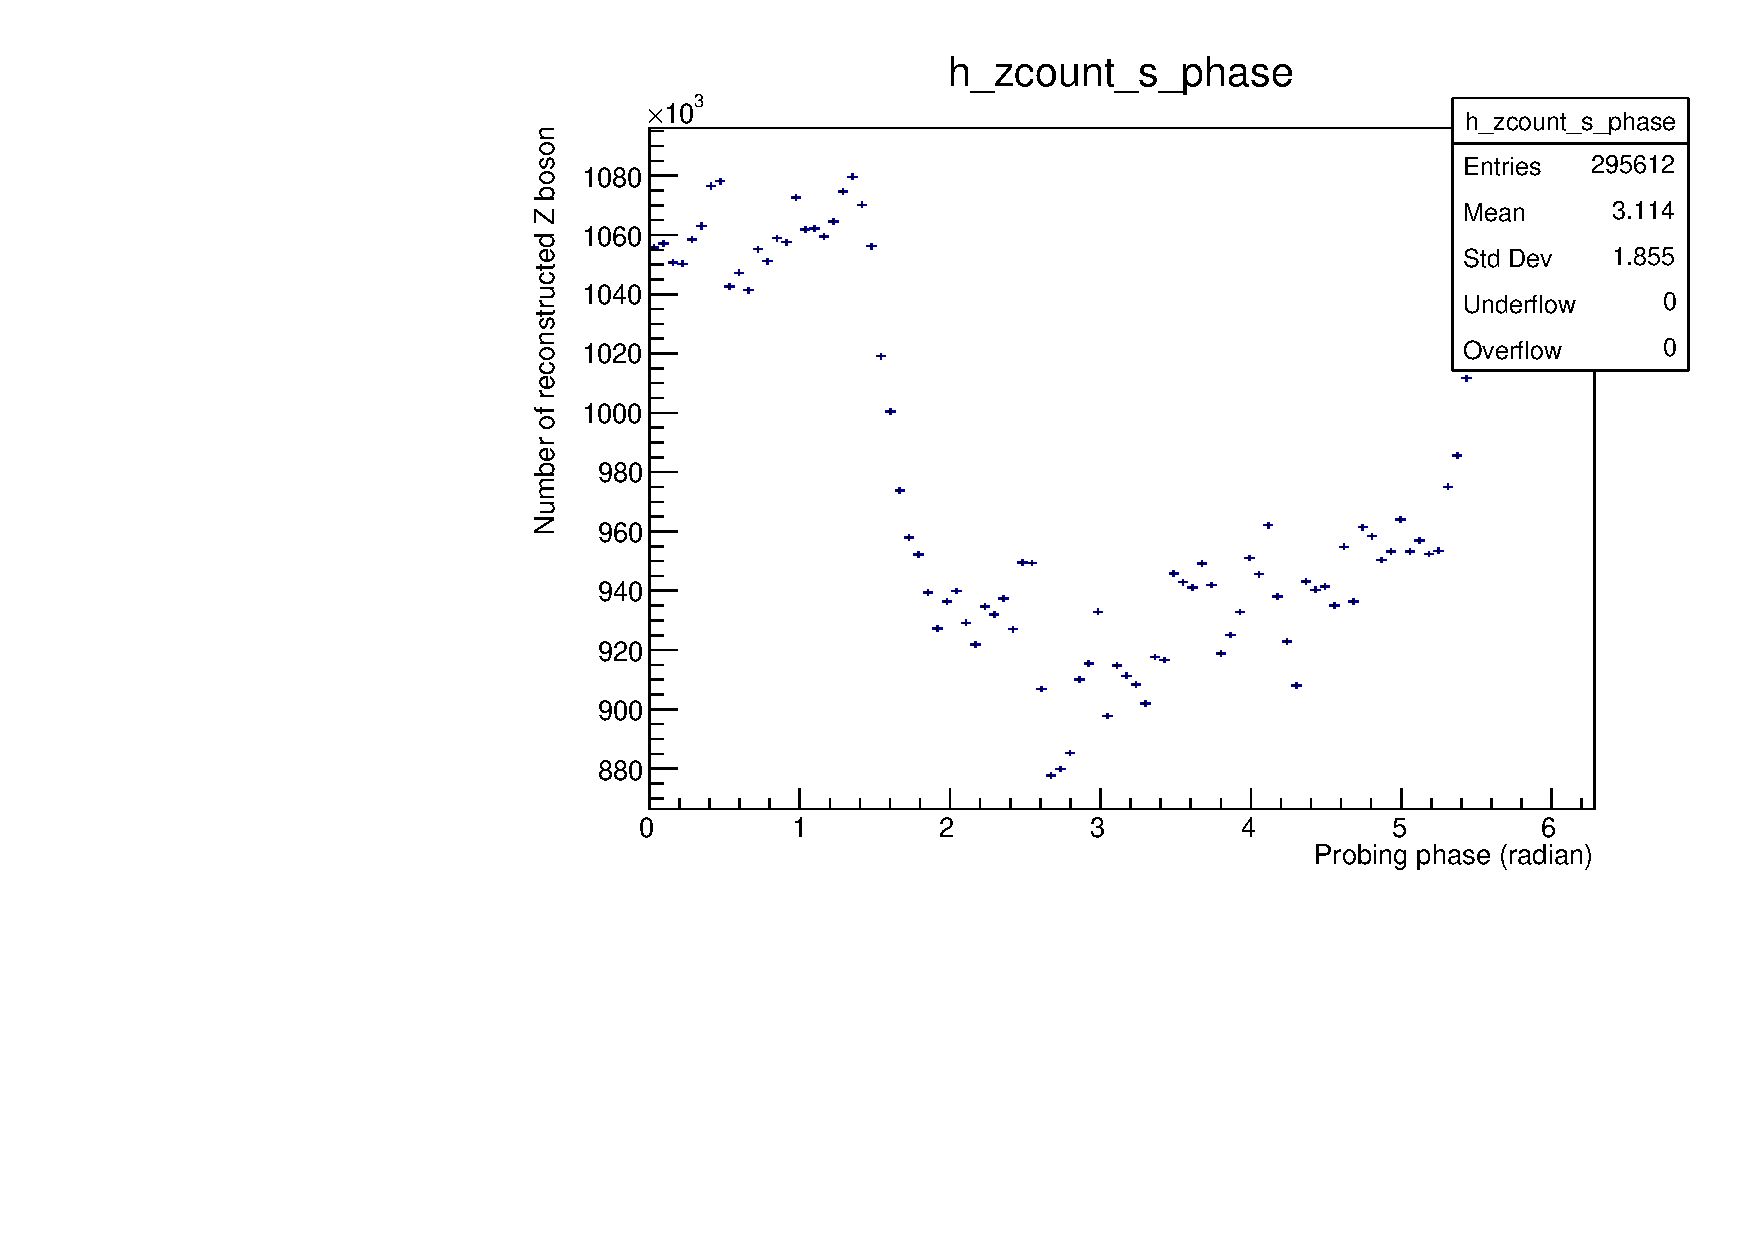
\includegraphics[width=0.4\textwidth]{figs/toy/fig_bin100_LIVxsec_0_random1_period1000_probe24_SigConfig0_LumiProf0_h_zcount_s_phase.pdf}
\caption{\label{fig:toy_numZ_phase} Integrated Lumiminoisty (left) and number of Z boson (right) for each sidereal phase bin (100 bins over 2$\pi$.) }
\end{figure}

In order to probe tiny effect, we take the double ratio as Eq.~\ref{eq:double_ratio}. 
The distribution of the double ratio is shown in Fig.~\ref{fig:toy_Dratio_phase}. 
On this TOY configuration, $\mathcal{L}_{int} = 178.2 fb^{-1}$, because we assume a flat instanteneous luminosity.

\begin{figure}
\centering
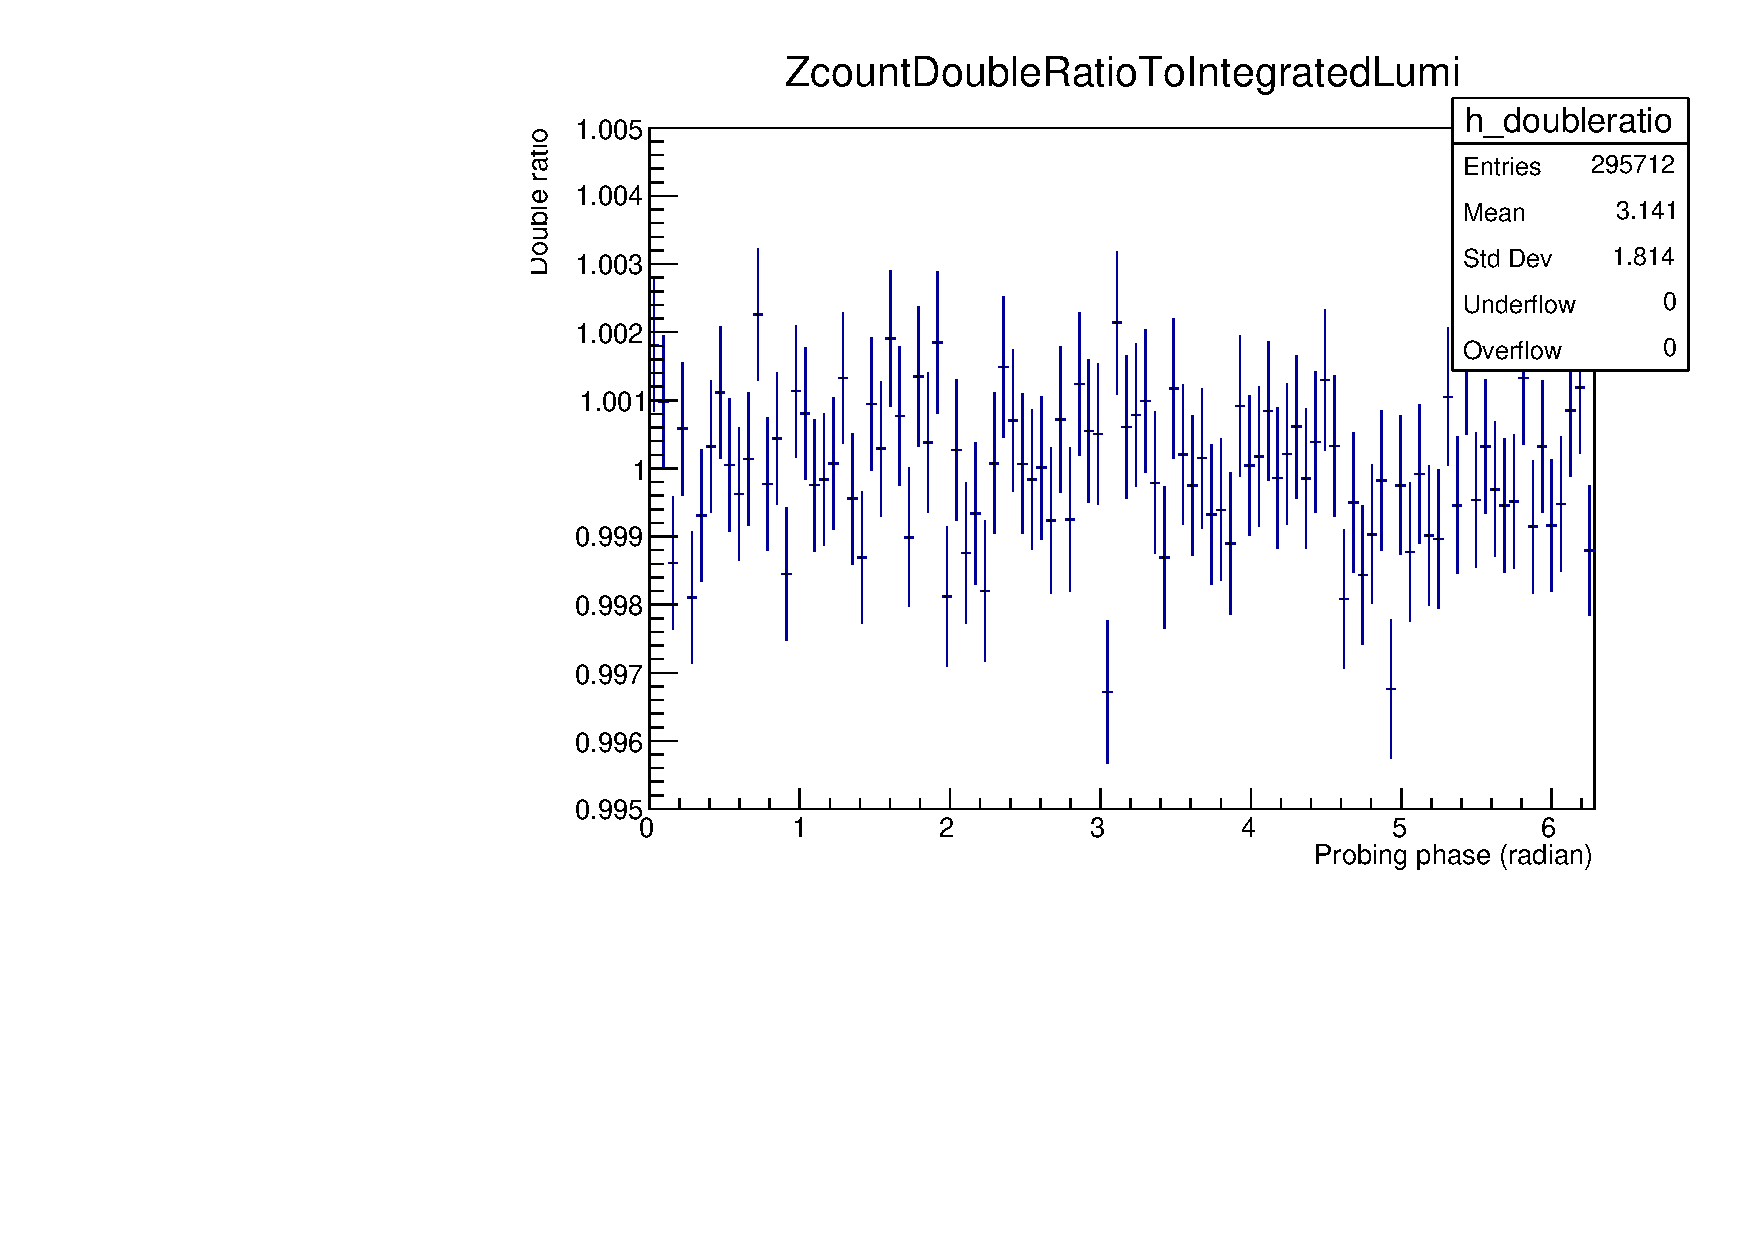
\includegraphics[width=0.4\textwidth]{figs/toy/fig_bin100_LIVxsec_0_random1_period1000_probe24_SigConfig0_LumiProf0_ZcountDoubleRatioToIntegratedLumi.pdf}
\caption{\label{fig:toy_Dratio_phase} The Double ratio for each sidereal phase bin (100 bins over 2$\pi$.) }
\end{figure}

Statistical uncertainties are shown in the error bar in Fig.~\ref{fig:toy_Dratio_phase}. In Figs.~\ref{fig:toy_Dratio_proj}, the projection of the double ratio and
 it's pull are shown. The mean and RMS of the pull distribution are consistent with 1.0, which shows reasonable error propagation has been made. 

\begin{figure}
\centering
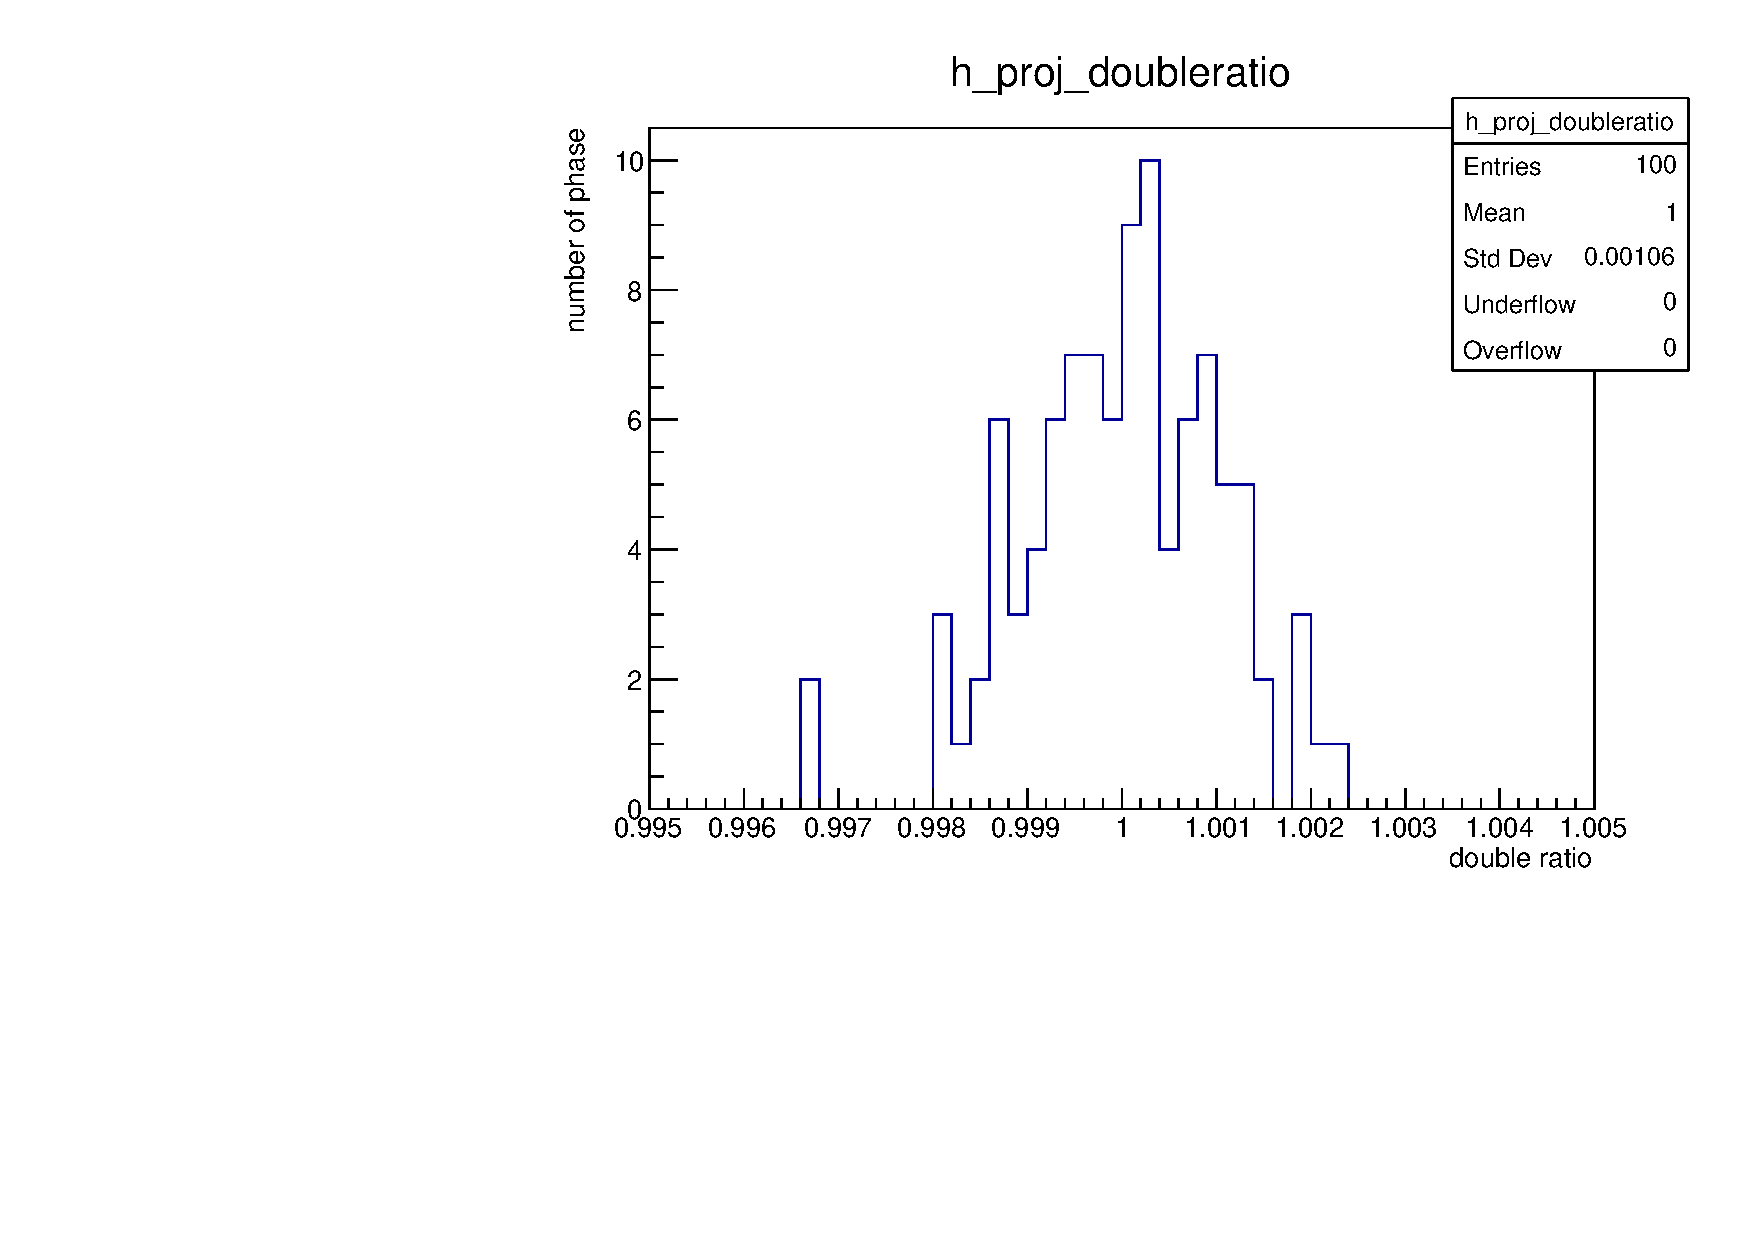
\includegraphics[width=0.4\textwidth]{figs/toy/fig_bin100_LIVxsec_0_random1_period1000_probe24_SigConfig0_LumiProf0_h_proj_doubleratio.pdf}
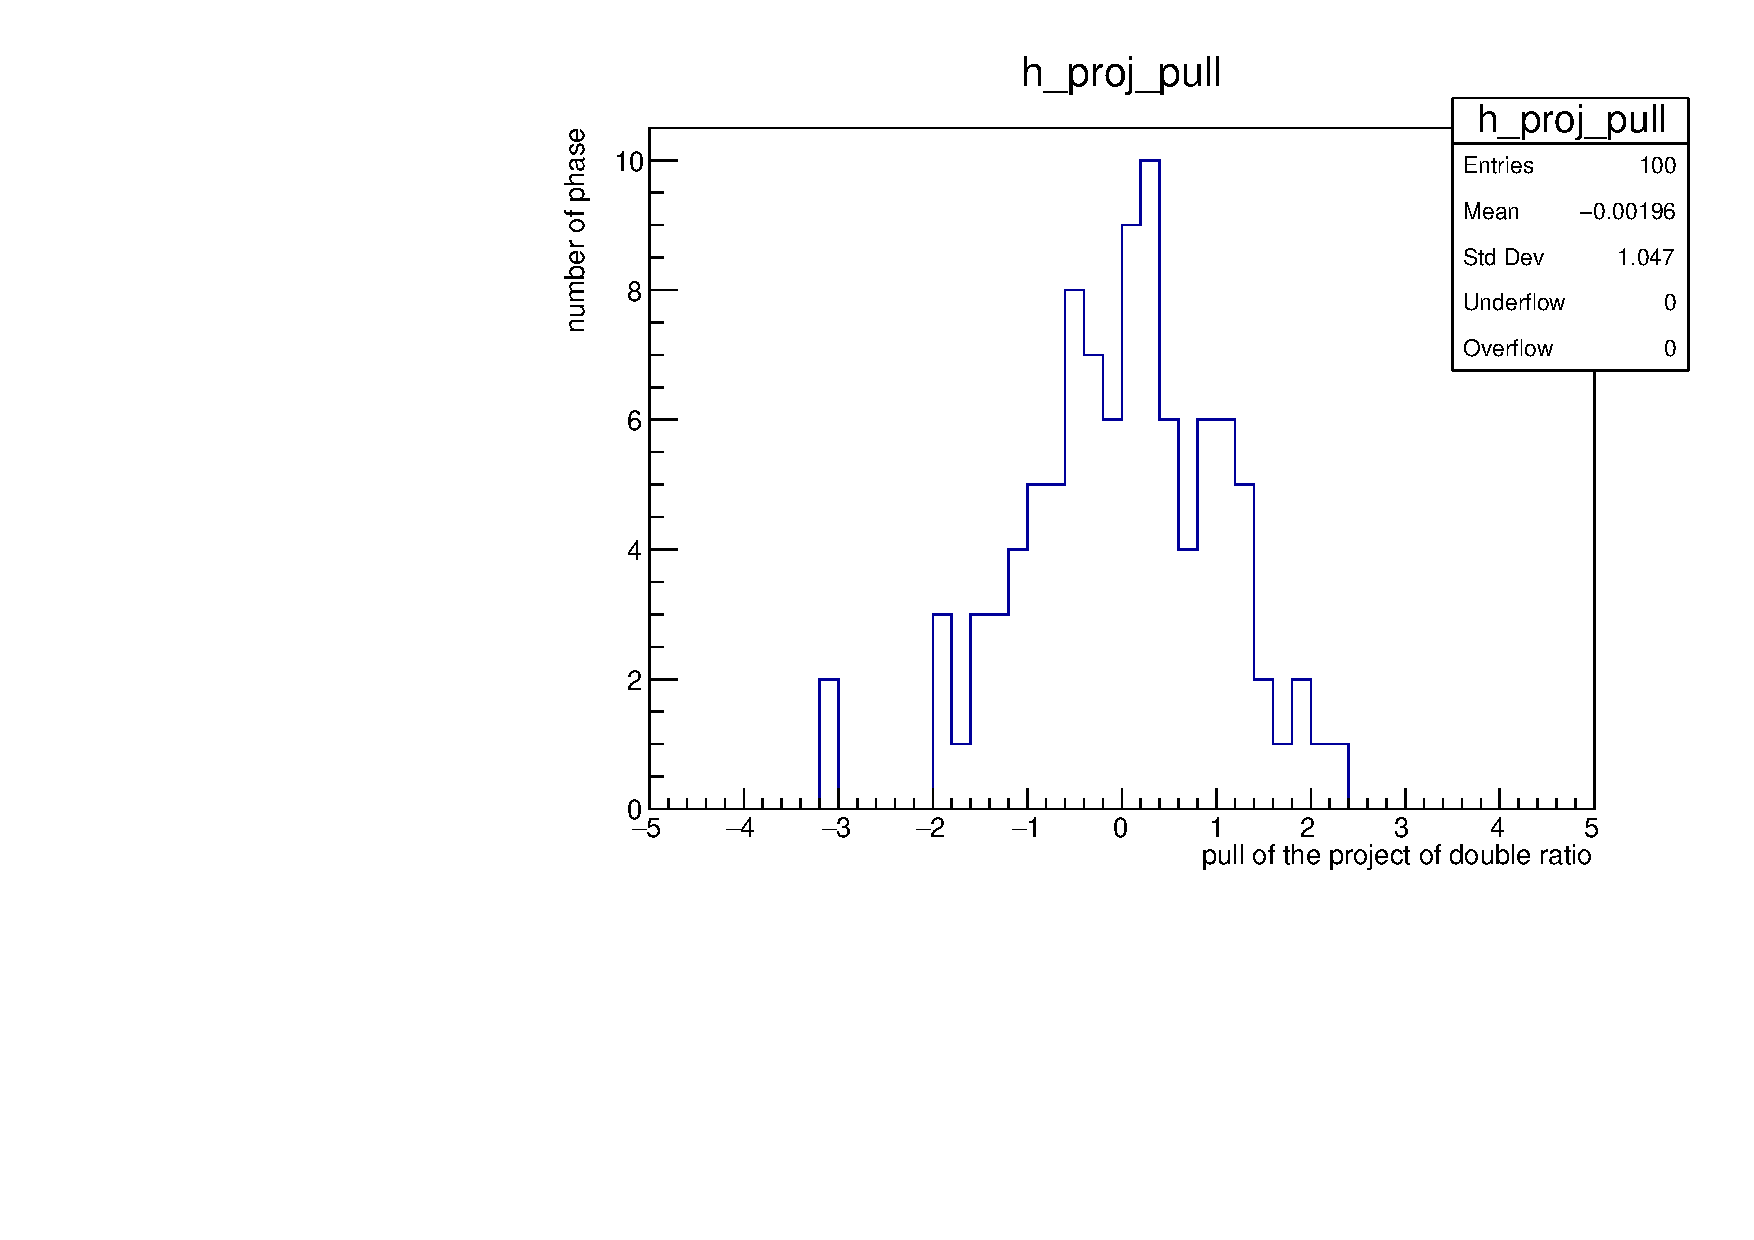
\includegraphics[width=0.4\textwidth]{figs/toy/fig_bin100_LIVxsec_0_random1_period1000_probe24_SigConfig0_LumiProf0_h_proj_pull.pdf}
\caption{\label{fig:toy_Dratio_proj} Projection of Fig.~\ref{fig:toy_Dratio_phase} (left) and pull distribution. }
\end{figure}



%% 
%% 
%% There are three types of TOY sample. 
%% \begin{enumerate}
%% \item[i] simplest: flat instanteneous luminosity (1.0 x $10^{34} cm^{-2}s^{-1}$) with time stamp of data lumi block.
%% \item[ii] data profile: data luminosity profile with with time stamp of data lumi block.
%% \item[iii] realistic: introduce additional efficiency degradation effect in addtion to (ii)
%% \end{enumerate}
%% 

%% \subsection{How the sidereal effect look like}

Figures ~\ref{fig:toy_Dratio_phase_s1pb} show the double ratio in case of LIV signal amplitude of 1 pb with sin wave. 
Just for illustration purpose, prepared with and without statistics fluctuation. 
The amplitude of no randome case is around 0.00133, which is from the cross section ratio of 1 pb over 750 pb, which is used to generate this Toy experiment.

\begin{figure}
\centering
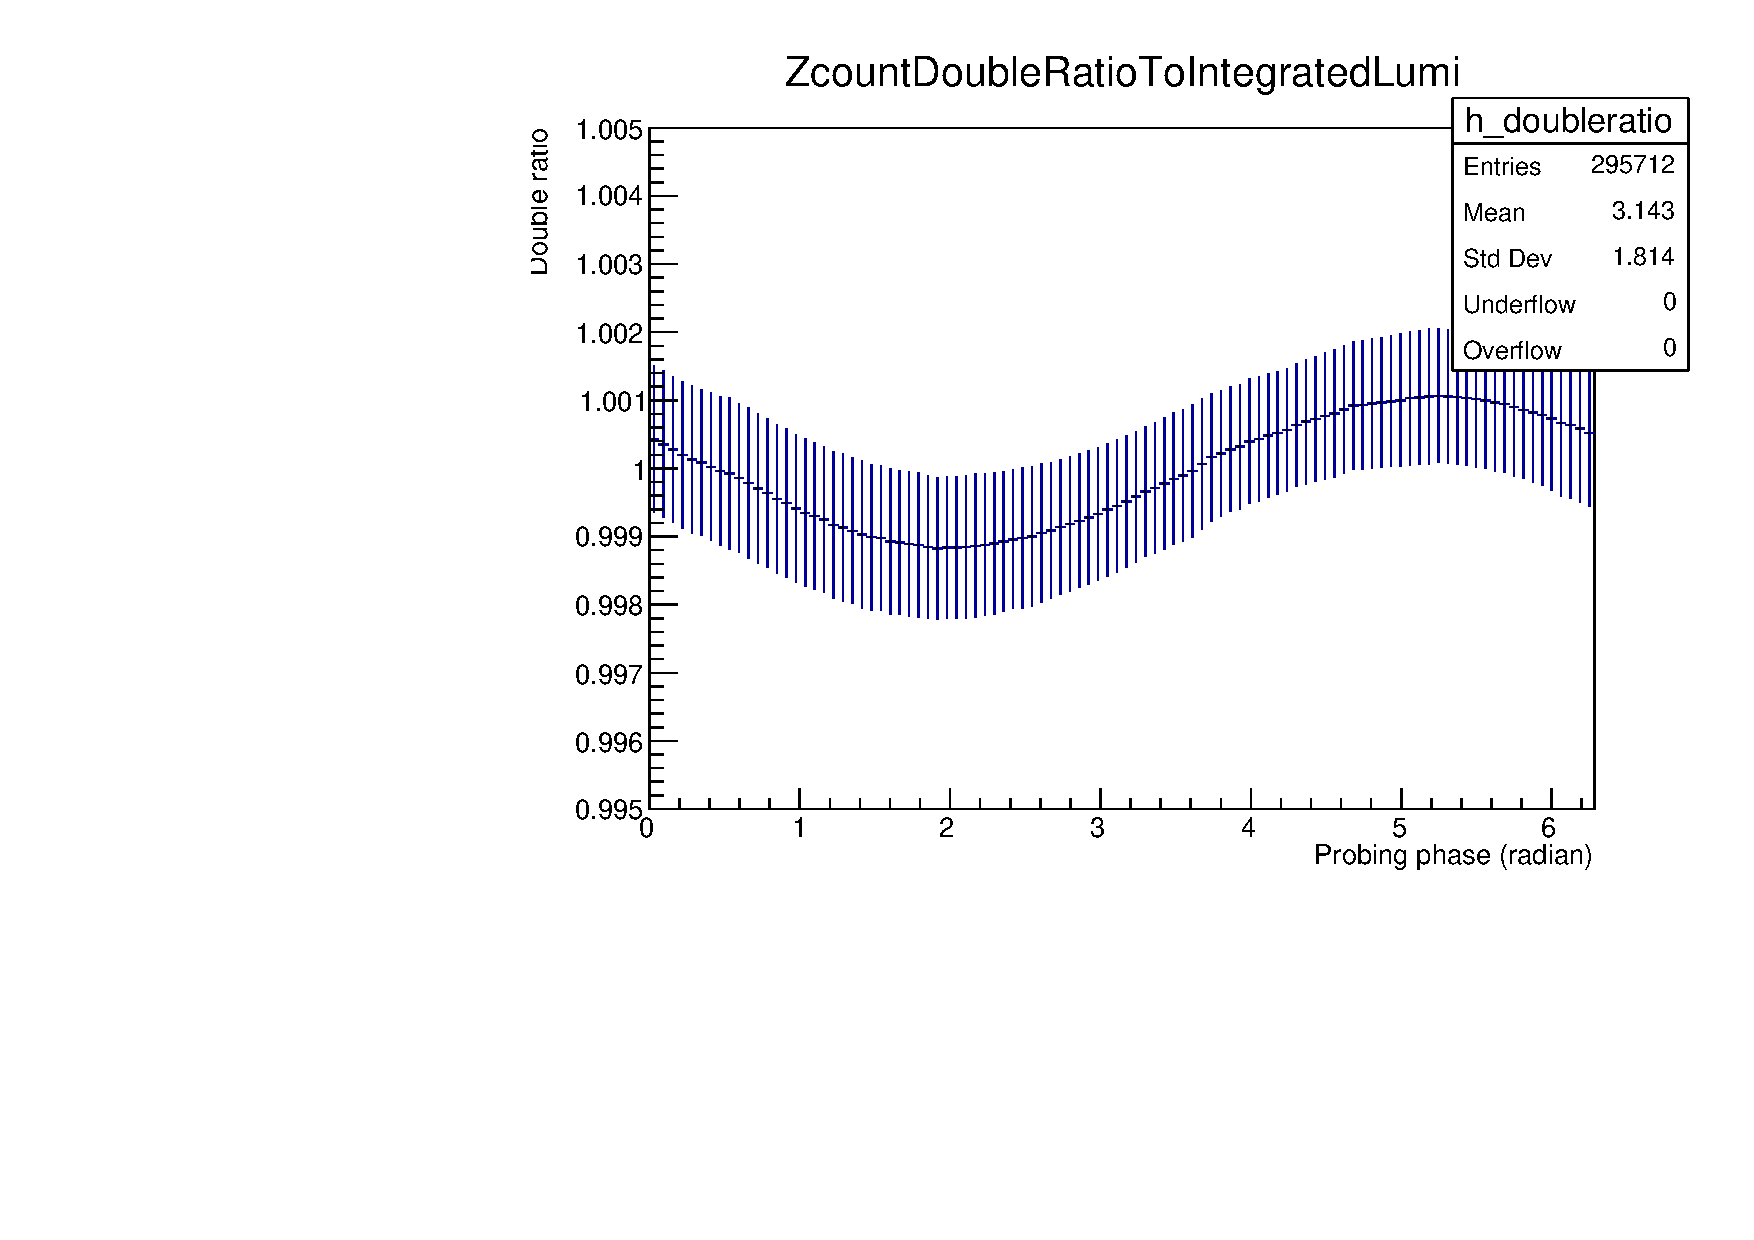
\includegraphics[width=0.4\textwidth]{figs/toy/fig_bin100_LIVxsec_1000_random0_period1000_probe24_SigConfig20_LumiProf0_ZcountDoubleRatioToIntegratedLumi.pdf}
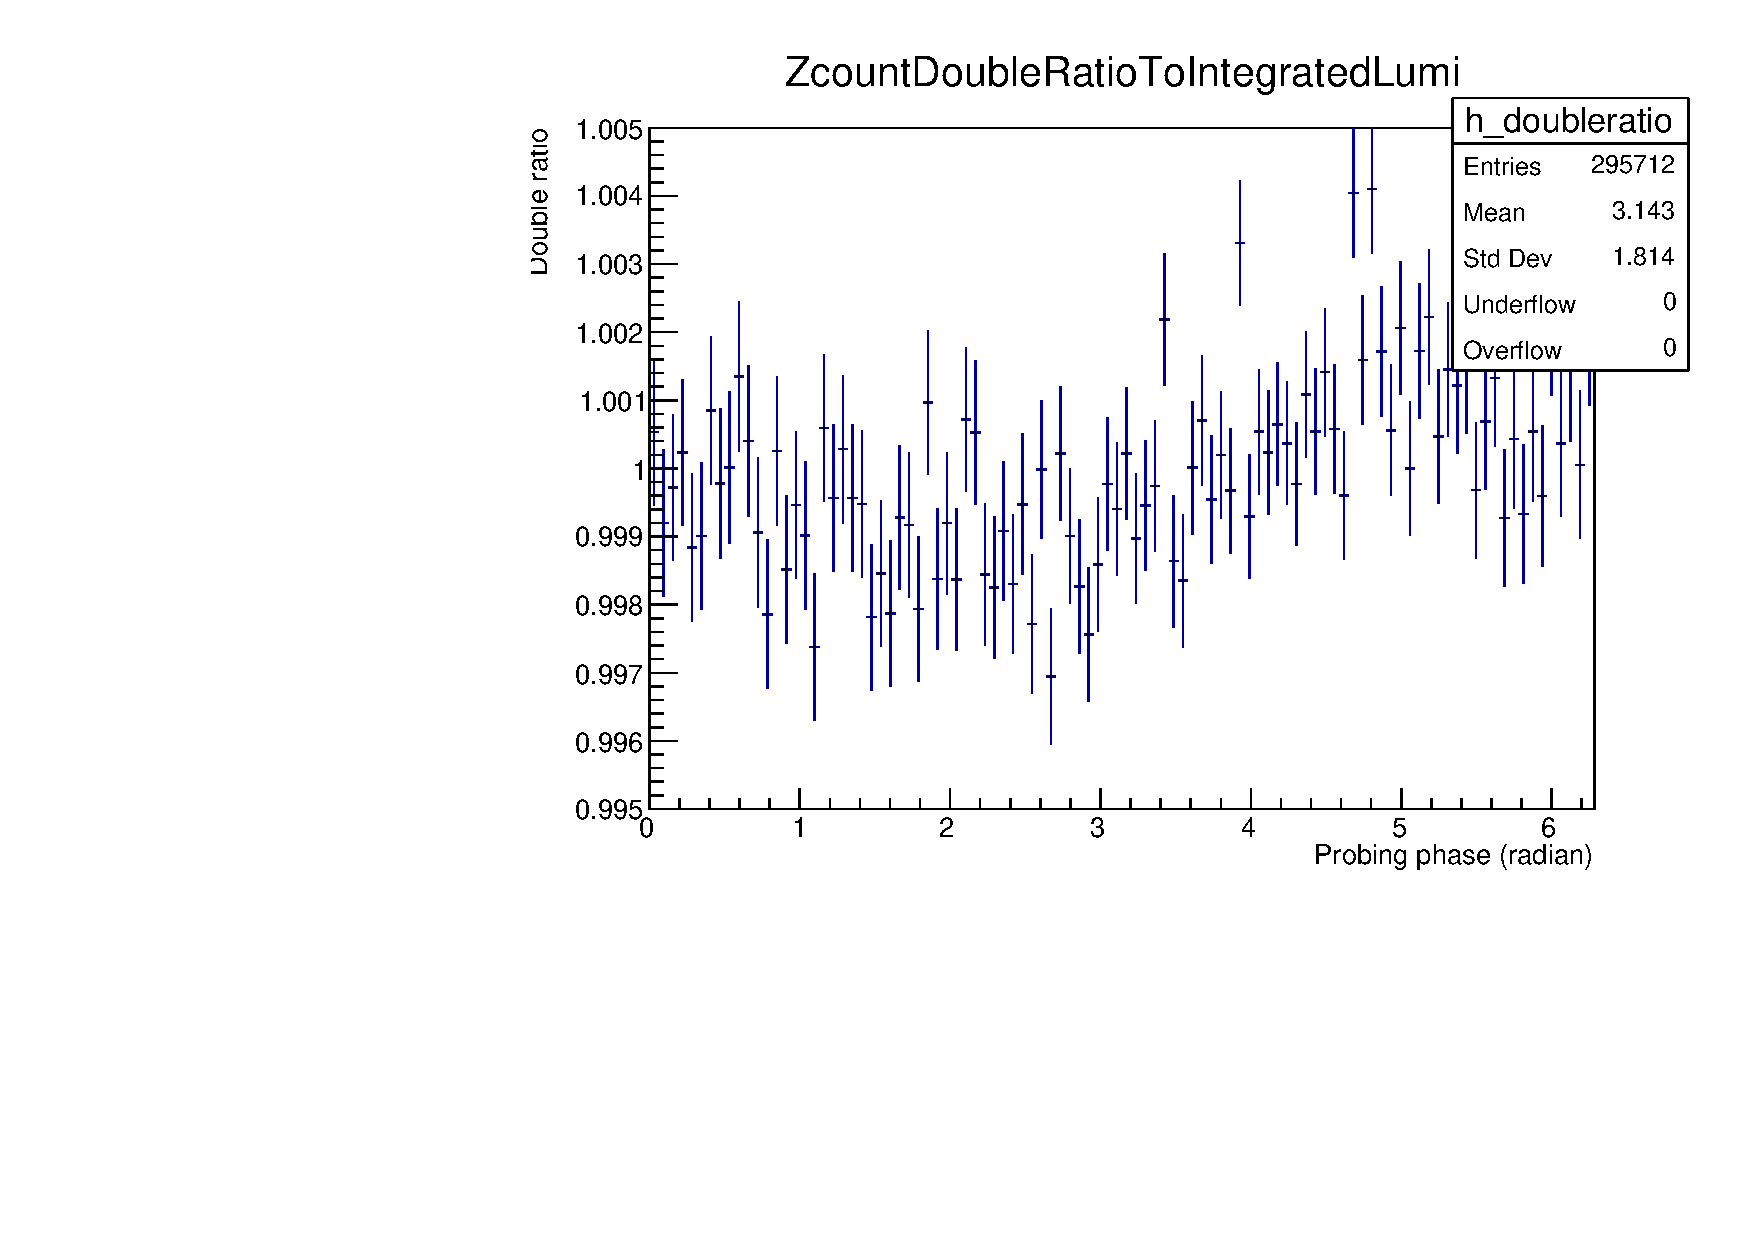
\includegraphics[width=0.4\textwidth]{figs/toy/fig_bin100_LIVxsec_1000_random1_period1000_probe24_SigConfig20_LumiProf0_ZcountDoubleRatioToIntegratedLumi.pdf}
\caption{\label{fig:toy_Dratio_phase_s1pb} The double ratio for each sidereal phase bin (100 bins over 2$\pi$.) with LIV signal amplitude of 1 pb. }
\end{figure}


\subsection{Study with TOY data}

 By using Toy data, some basic studies are performed. 

\subsubsection{No signal case}

 This is test on NULL signal hypothesis. Figure~\ref{fig:toy_Dratio_phase_null} shows the double ratio with NULL signal, for both with and without statistical fluctuation.
Based on this configuration, 1000 Toy experiments are generated and fit simple sin and cosin curve. The results of these fit are shown in Fig.~\ref{fig:toy_1000exp_s0pb}. 
Mean value are consistent with zero, and the RMS is 0.00012. From this, we have statistical limit around 10 to -4. 

\begin{figure}
\centering
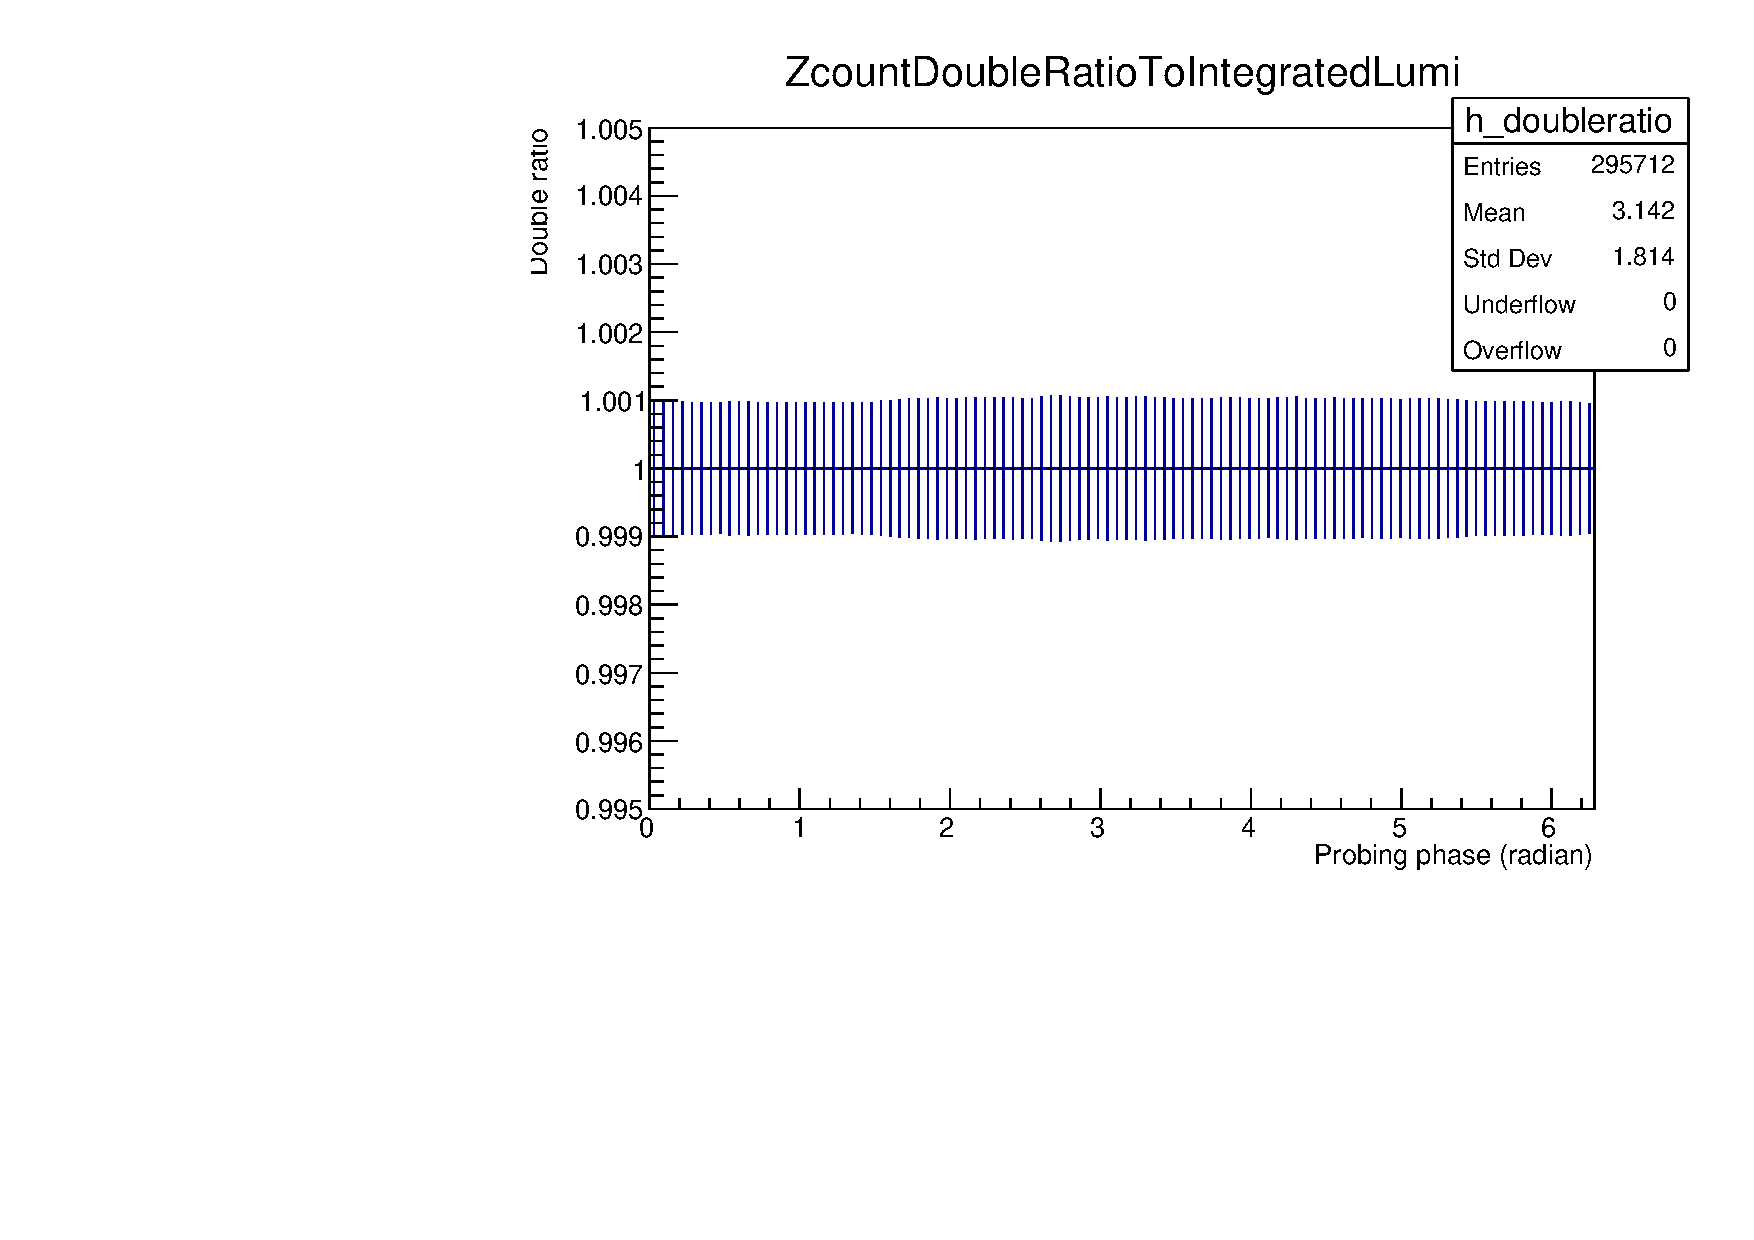
\includegraphics[width=0.4\textwidth]{figs/toy/fig_bin100_LIVxsec_0_random0_period1000_probe24_SigConfig0_LumiProf0_ZcountDoubleRatioToIntegratedLumi.pdf}
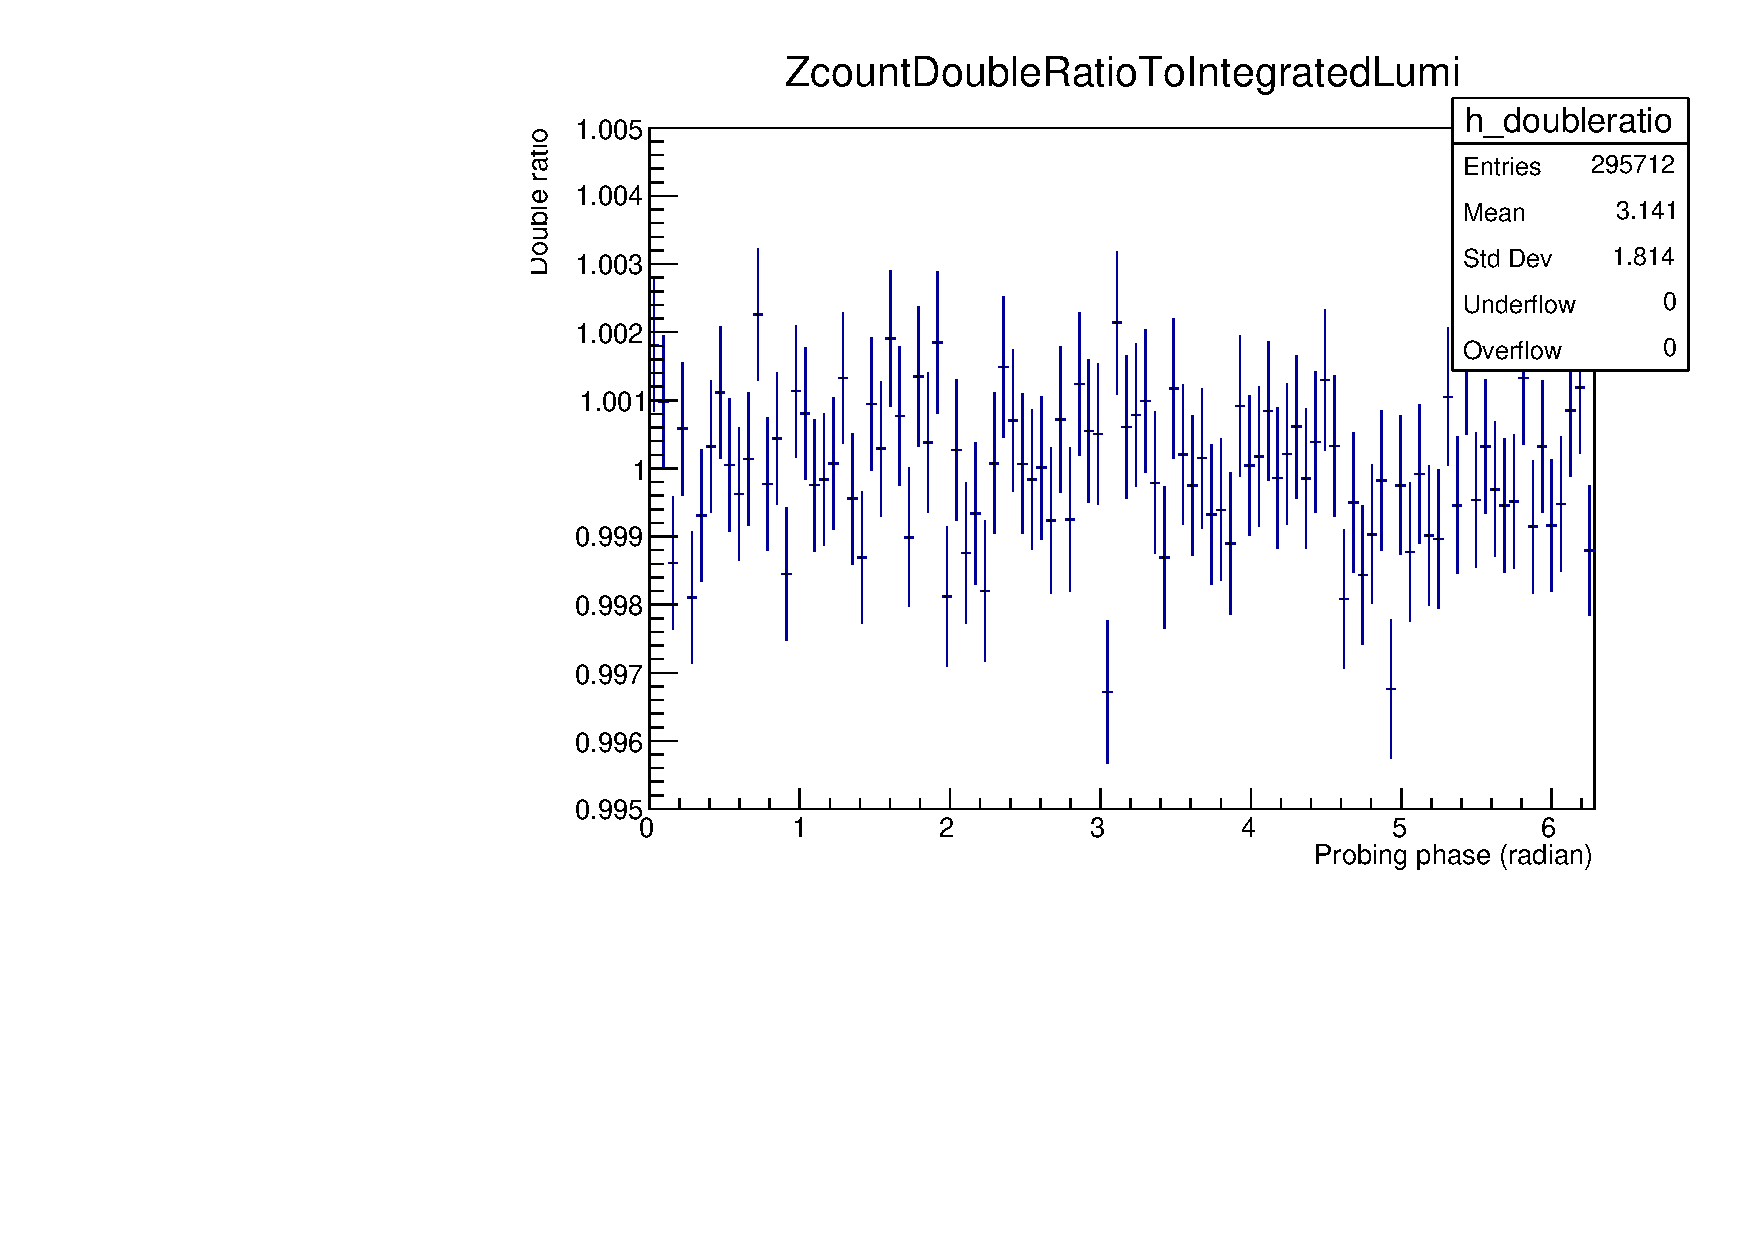
\includegraphics[width=0.4\textwidth]{figs/toy/fig_bin100_LIVxsec_0_random1_period1000_probe24_SigConfig0_LumiProf0_ZcountDoubleRatioToIntegratedLumi.pdf}
\caption{\label{fig:toy_Dratio_phase_null} The double ratio for each sidereal phase bin (100 bins over 2$\pi$.) with LIV signal amplitude of 0 pb (NULL signal). }
\end{figure}


\begin{figure}
\centering
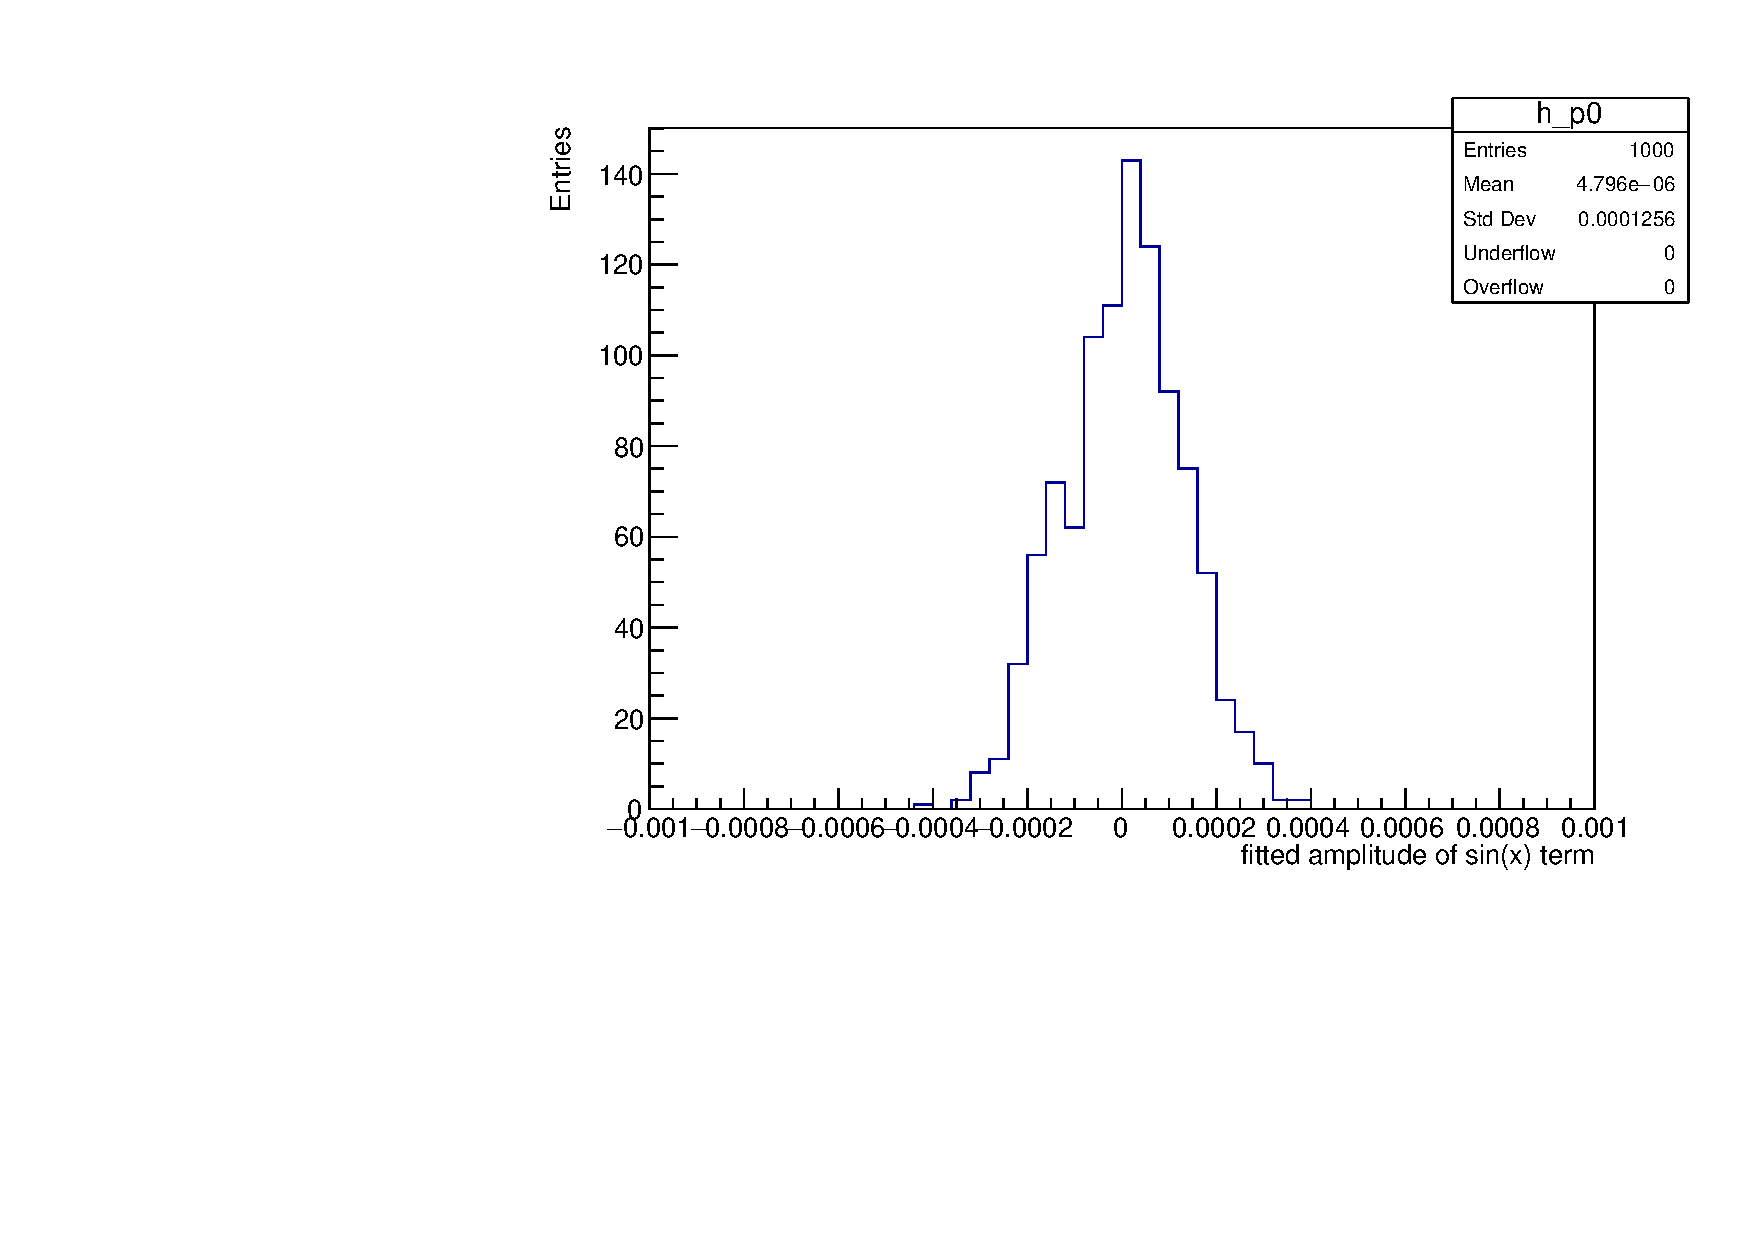
\includegraphics[width=0.4\textwidth]{figs/toy/res_1000_toy_nosignal_p0.pdf}
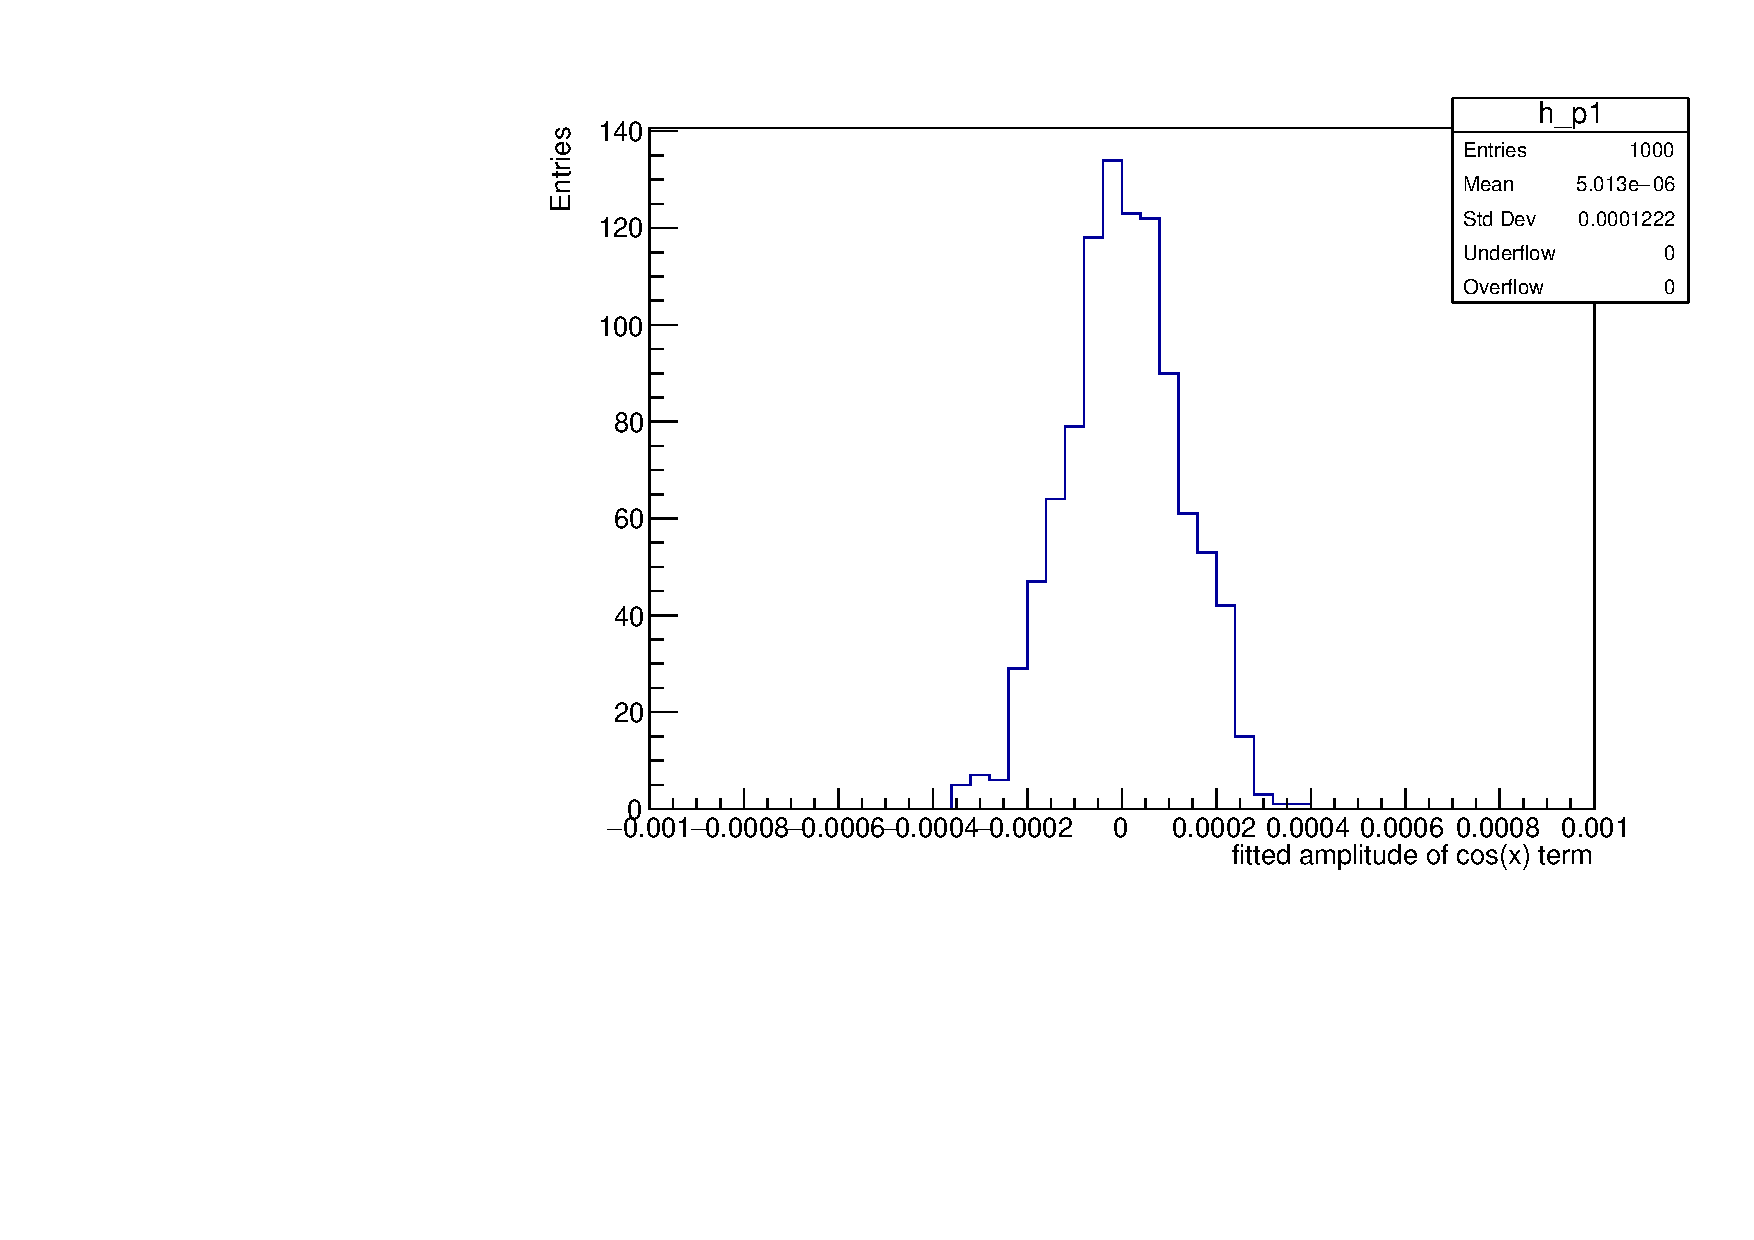
\includegraphics[width=0.4\textwidth]{figs/toy/res_1000_toy_nosignal_p1.pdf}
\caption{\label{fig:toy_1000exp_s0pb} Result of 1000 toy experiement with NULL signal. Fit function is 1 + p0 sin(x)+p1 cos(x). (left) amplitude of sin(x) term, (right) amplitude of cos(x). }
\end{figure}

%\clearpage
%% \subsection{Null hypothesis test}
\label{sec:null_test}

%% Null test is that we perform a fit to data (toy datasets) using SM expectation. 
%% The SM expectation is a flat distribution in which free parameter is an offset (e.g $y = c $).

In this test, 1000 toy datasets generated with SM expection and corresponds 
to Run 2 datase are used. In another words, no signal is injected to these datasets.

Figure~\ref{fig:null_test} show distributions of fit parameters, errors,
$\chi^{2}/ndf$ (ndf is number of degree of freedom) and  $p_{0}$ value of
$\chi^{2}$, from fitting a flat distribution (bkg expection) to the 1000
toy datasets. Since the obserable is a Double Ratio, the fitted off-set (fit parameter)
is allways one in each fit. The normalzed $\chi^{2}$ ($\chi^{2}/ndf$, bottom right plot)
distribution is centered around one which means the toy datasets agree
with a flat distribution (this is what we expected). If we take  $p_0$ > 0.01 as a threshold to determine
if the dataset agree with the SM expectation (flat distribution), then more then 99\% of the toy dataset
passed this cut ($p_0$ > 0.01 ). Since more then 99\% of the samples agree with SM expectation we can conclude
that random fluctuation can not introduce strange shapes that significantly different then a flat distribution.

\begin{figure}[!htb]
  \centering
  \subfloat{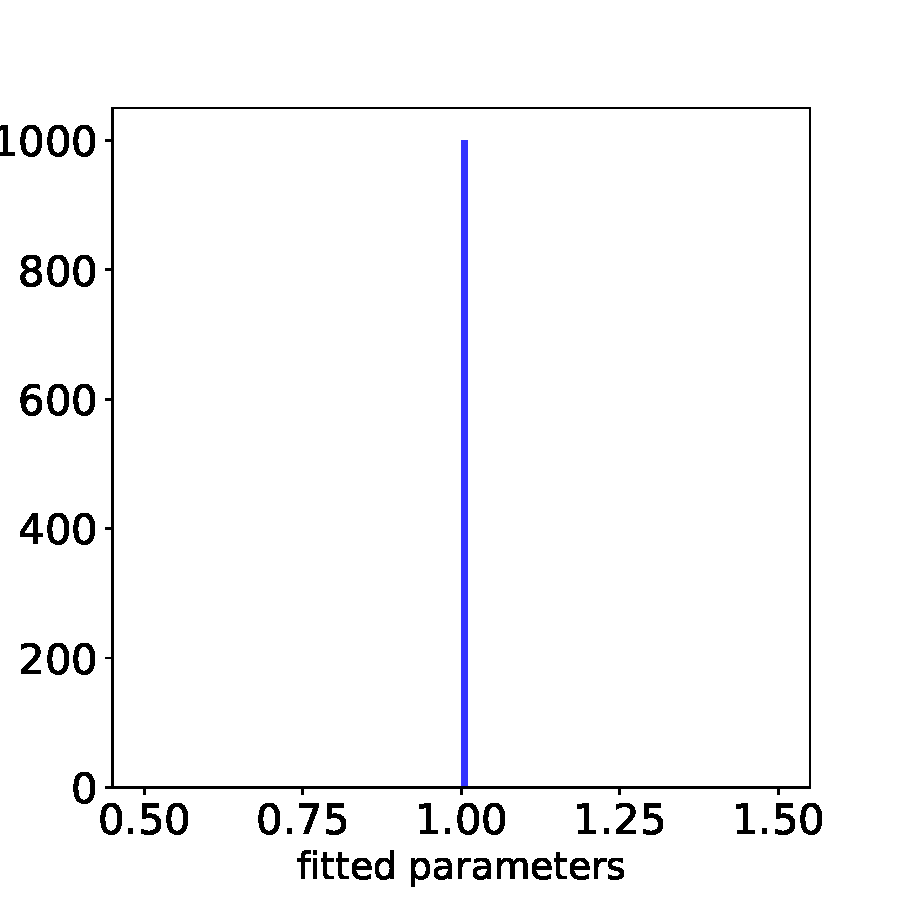
\includegraphics[width=0.40\textwidth]{figs/null_test/Null_test_pars}}
  \subfloat{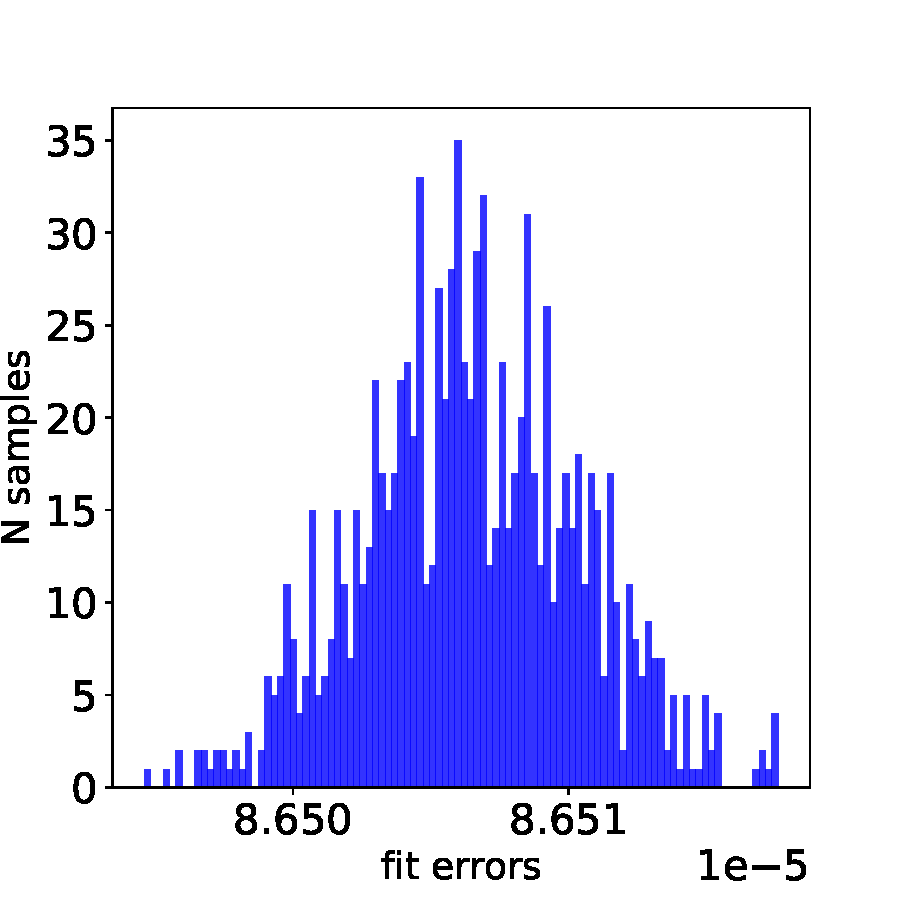
\includegraphics[width=0.40\textwidth]{figs/null_test/Null_test_err}}\\
  \subfloat{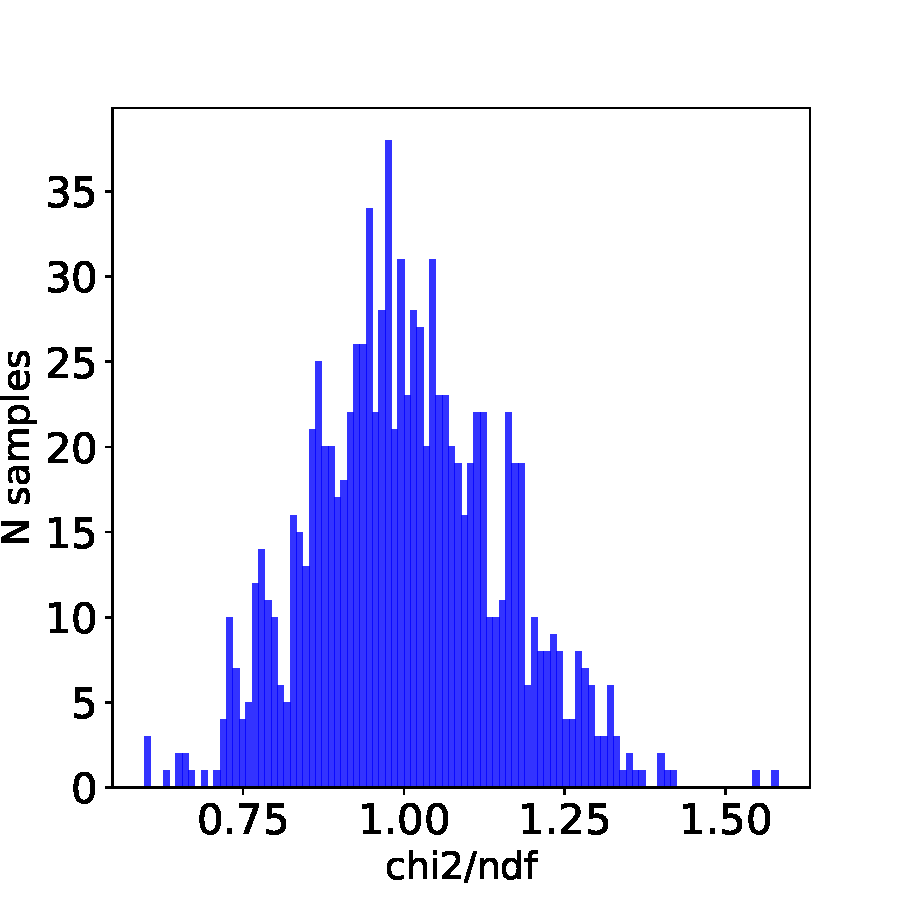
\includegraphics[width=0.40\textwidth]{figs/null_test/Null_test_chi2_ndf}}
  \subfloat{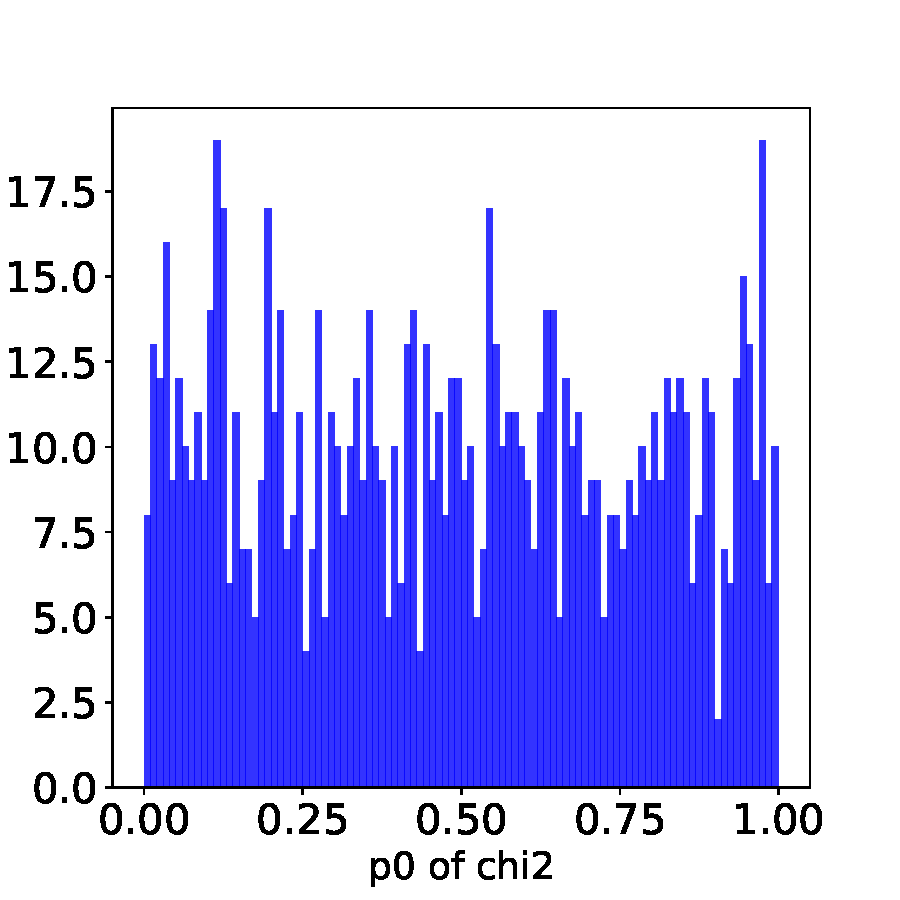
\includegraphics[width=0.40\textwidth]{figs/null_test/Null_test_chi2_p0}}
  \caption{Results of Null Tests on 1000 signal-free toy datasets. Top left plot is estimated parameters, top right is fit errors, bottom left is $\chi^{2}/ndf$ (ndf is number of degree of freedom), bottom right is $p_{0}$ of $\chi^{2}$.}
  \label{fig:null_test}
\end{figure}



%\clearpage
\subsection{Spurious signal test}
\label{sec:spurious_test}

Spurious signals may occur from statistical fluctuations. Therefore, in this section, we test toy datasets to check if there are signal like structures. The toy datasets are signal-free datasets (no signals injected), and generated total of 1000 samples. Each sample (toy dataset) is fitted 12 times, each time with different signal shapes (we have total of 12 signals). Each fit will estimate a coefficient. 

Figure~\ref{fig:spurious_test} shows distributions of 4 example coefficients ($d_u^{XZ}\equiv d_{0}$, $d_u^{YZ} \equiv d_{1}$, $d_u^{XX-YY} \equiv d_{2}$ and $d_u^{XY} \equiv d_{3}$) estimated from 1000 toy datasets. From each plot we can see that mean of each distribution is very close to zero. The Figure~\ref{fig:spurious_test_summary} shows mean and standard deviation of the distributions shown in Figure~\ref{fig:spurious_test}, expanded to all 12 coefficients.



\begin{figure}[!htb]
	\centering
	\subfloat{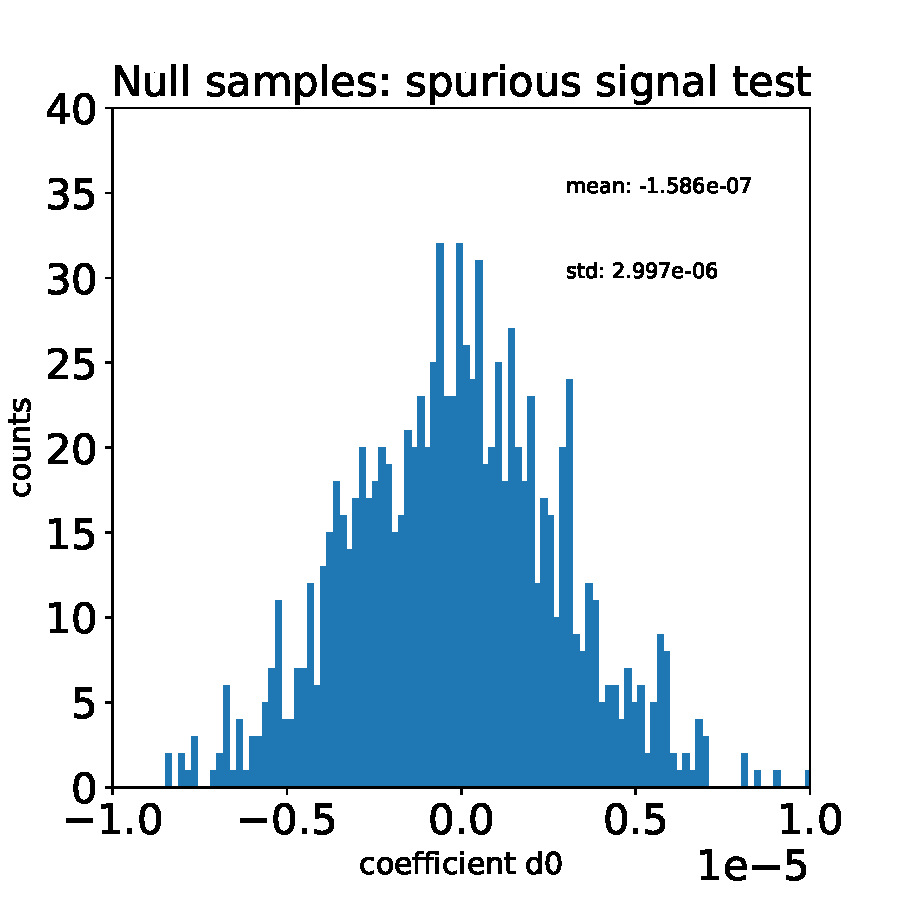
\includegraphics[width=0.48\textwidth]{figs/spurious_test/Null_spurious_test_d0}}
	\subfloat{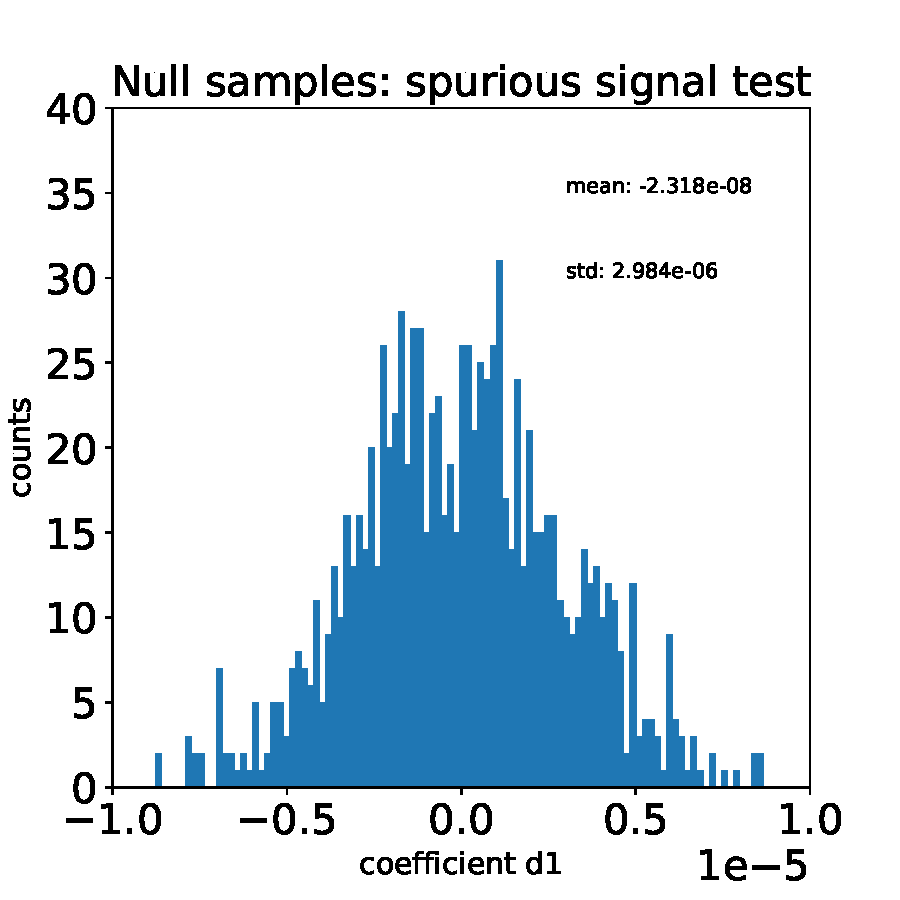
\includegraphics[width=0.48\textwidth]{figs/spurious_test/Null_spurious_test_d1}}\\
	\subfloat{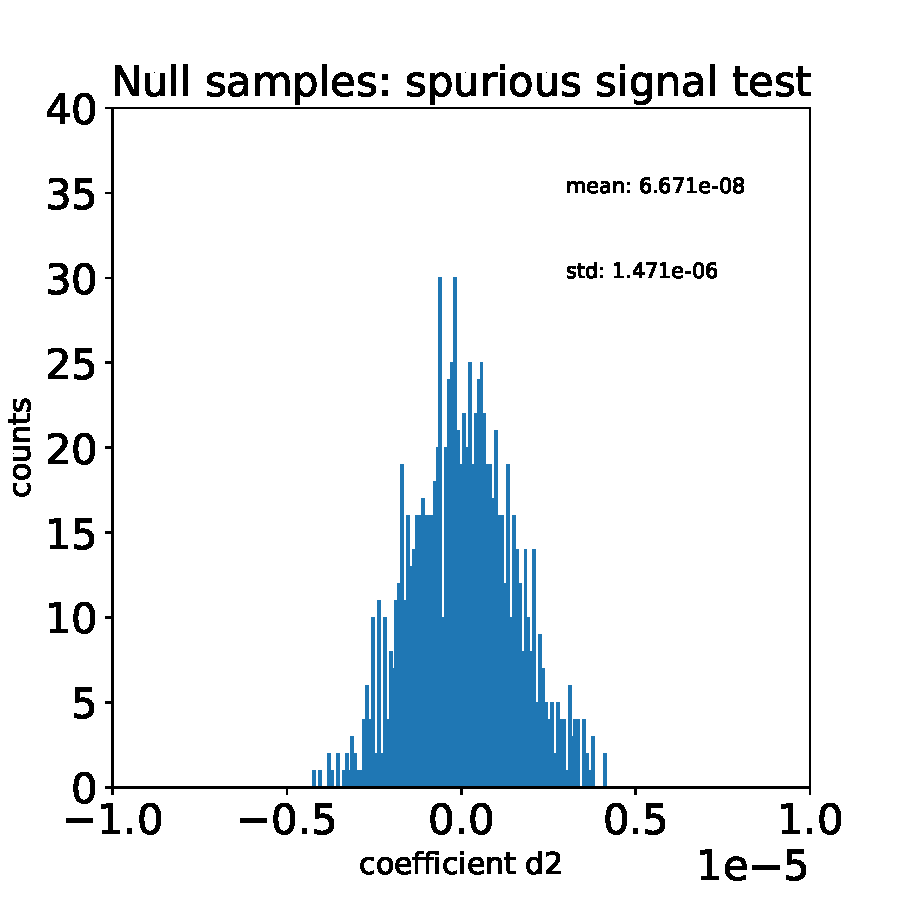
\includegraphics[width=0.48\textwidth]{figs/spurious_test/Null_spurious_test_d2}}
	\subfloat{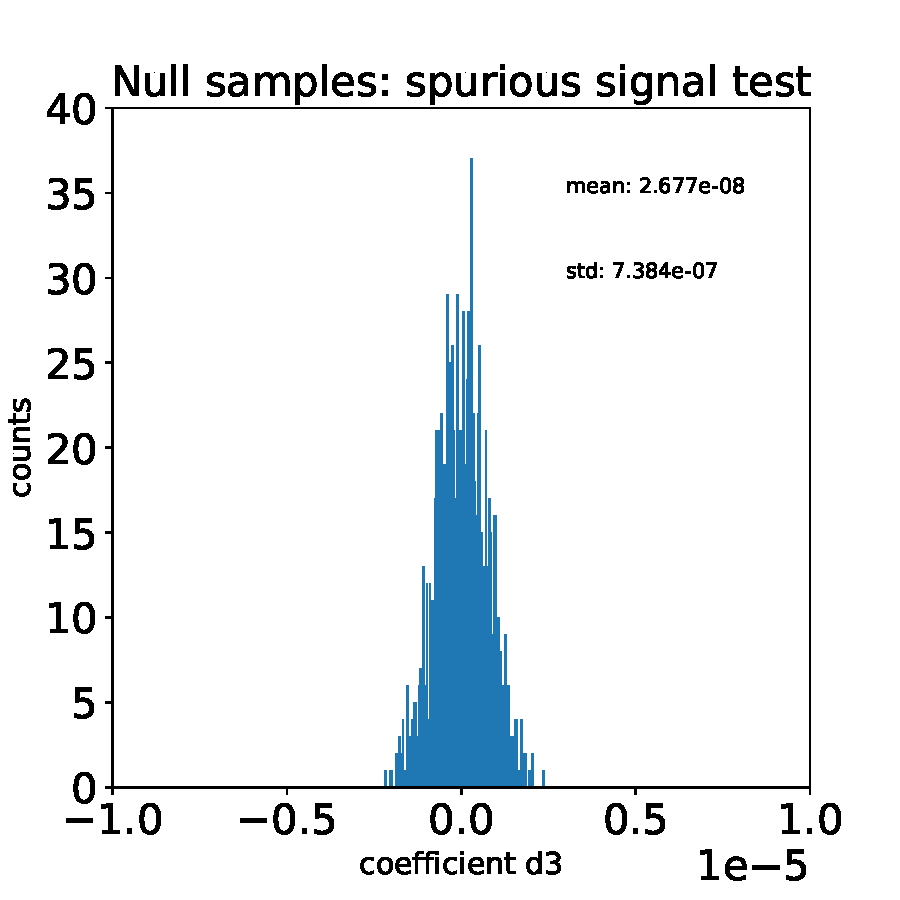
\includegraphics[width=0.48\textwidth]{figs/spurious_test/Null_spurious_test_d3}}
    \caption{Results of spurious signal tests on 1000 signal-free toy datasets. Top left is a distribution of estimated $d_{0}$ parameters, top right is $d_{1}$ parameters, bottom left is $d_{2}$ parameters and bottom right is $d_{3}$ parameters.}
	\label{fig:spurious_test}
\end{figure}


\begin{figure}[!htb]
	\centering
	\subfloat{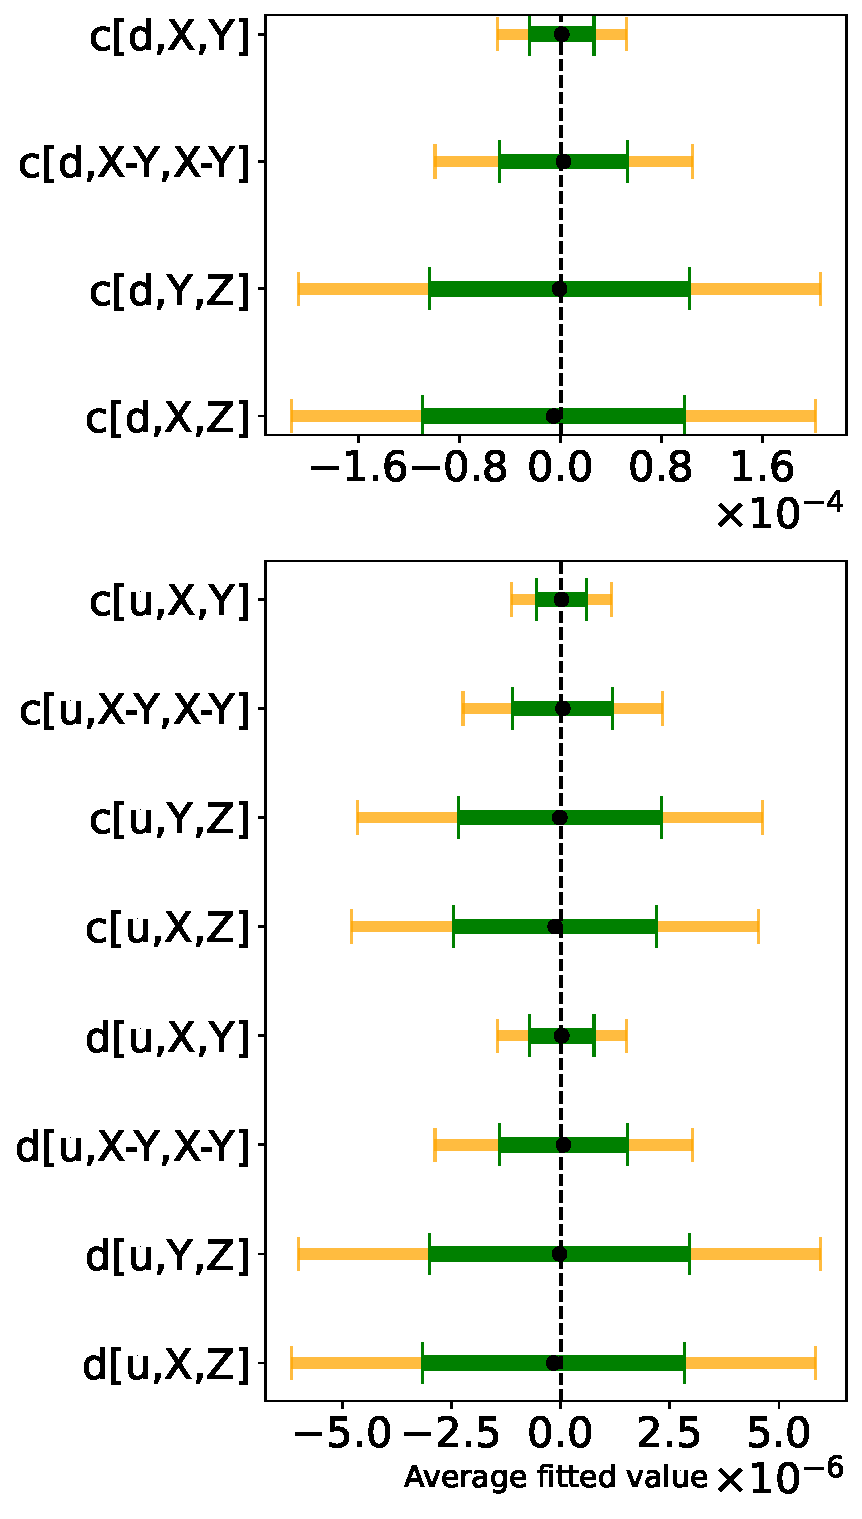
\includegraphics[width=0.48\textwidth]{figs/spurious_test/Null_SigFit_summary_1000samples}}

     \caption{Summary of spurious signal tests on 1000 signal-free toy datasets. Black dot is a numpy mean of corresponding distributions
       in the Figure~\ref{fig:spurious_test}, the green and orange bands are one and two standard diviations calculated with the numpy function. }
	\label{fig:spurious_test_summary}
\end{figure}



\subsubsection{Simple LIV effect}

 This is test with LIV signal amplitude of 1 pb with sin curve. 
Same as NULL case, 1000 toy experiments are generated as same method described in Section~\ref{sec:basic_TOYmodel}, and fitted with simple function. Results are shown in Fig.~\ref{fig:toy_1000exp_s1pb}
The mean of the fitted amplitude of sin (cos) term is 0.0013 (0.000), which is consistent with generated configuration. 

\begin{figure}
\centering
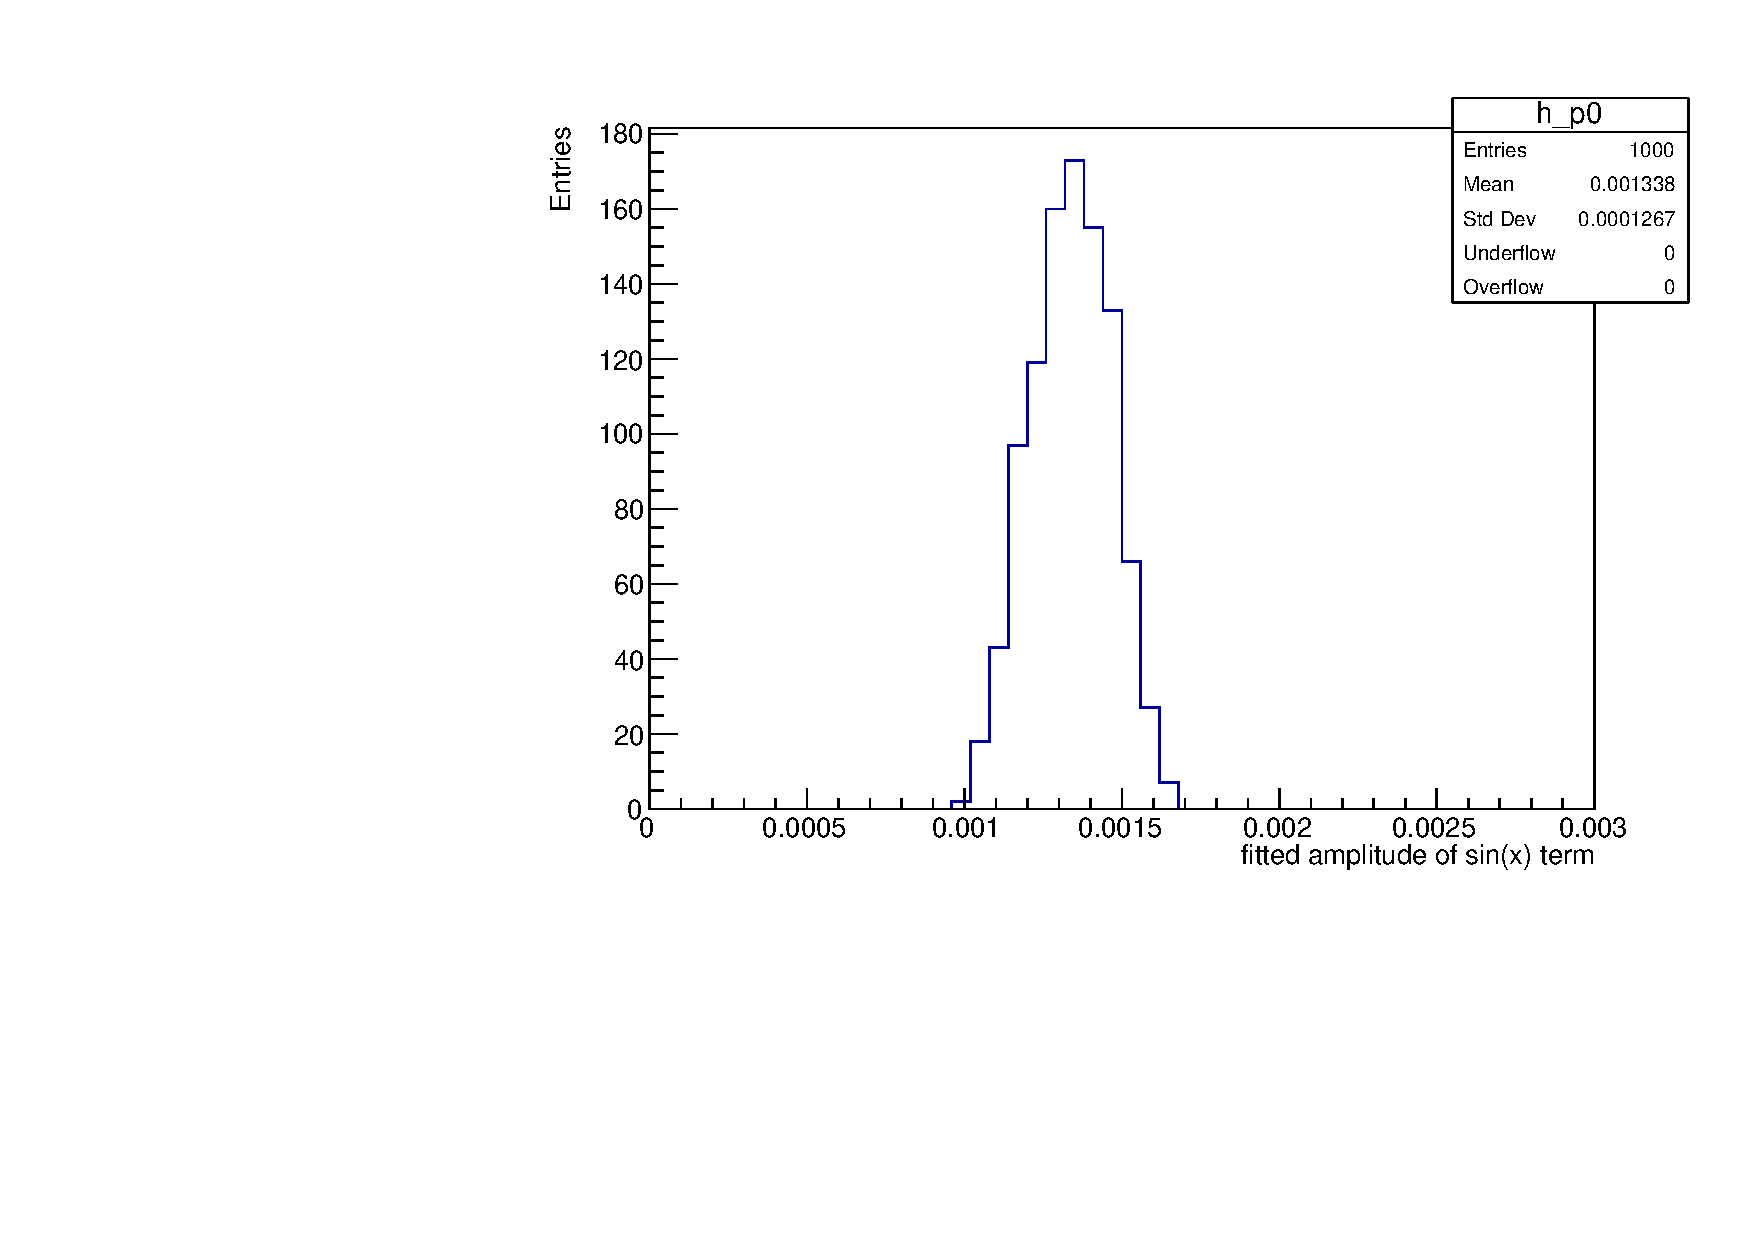
\includegraphics[width=0.4\textwidth]{figs/toy/res_1000_toy_p0.pdf}
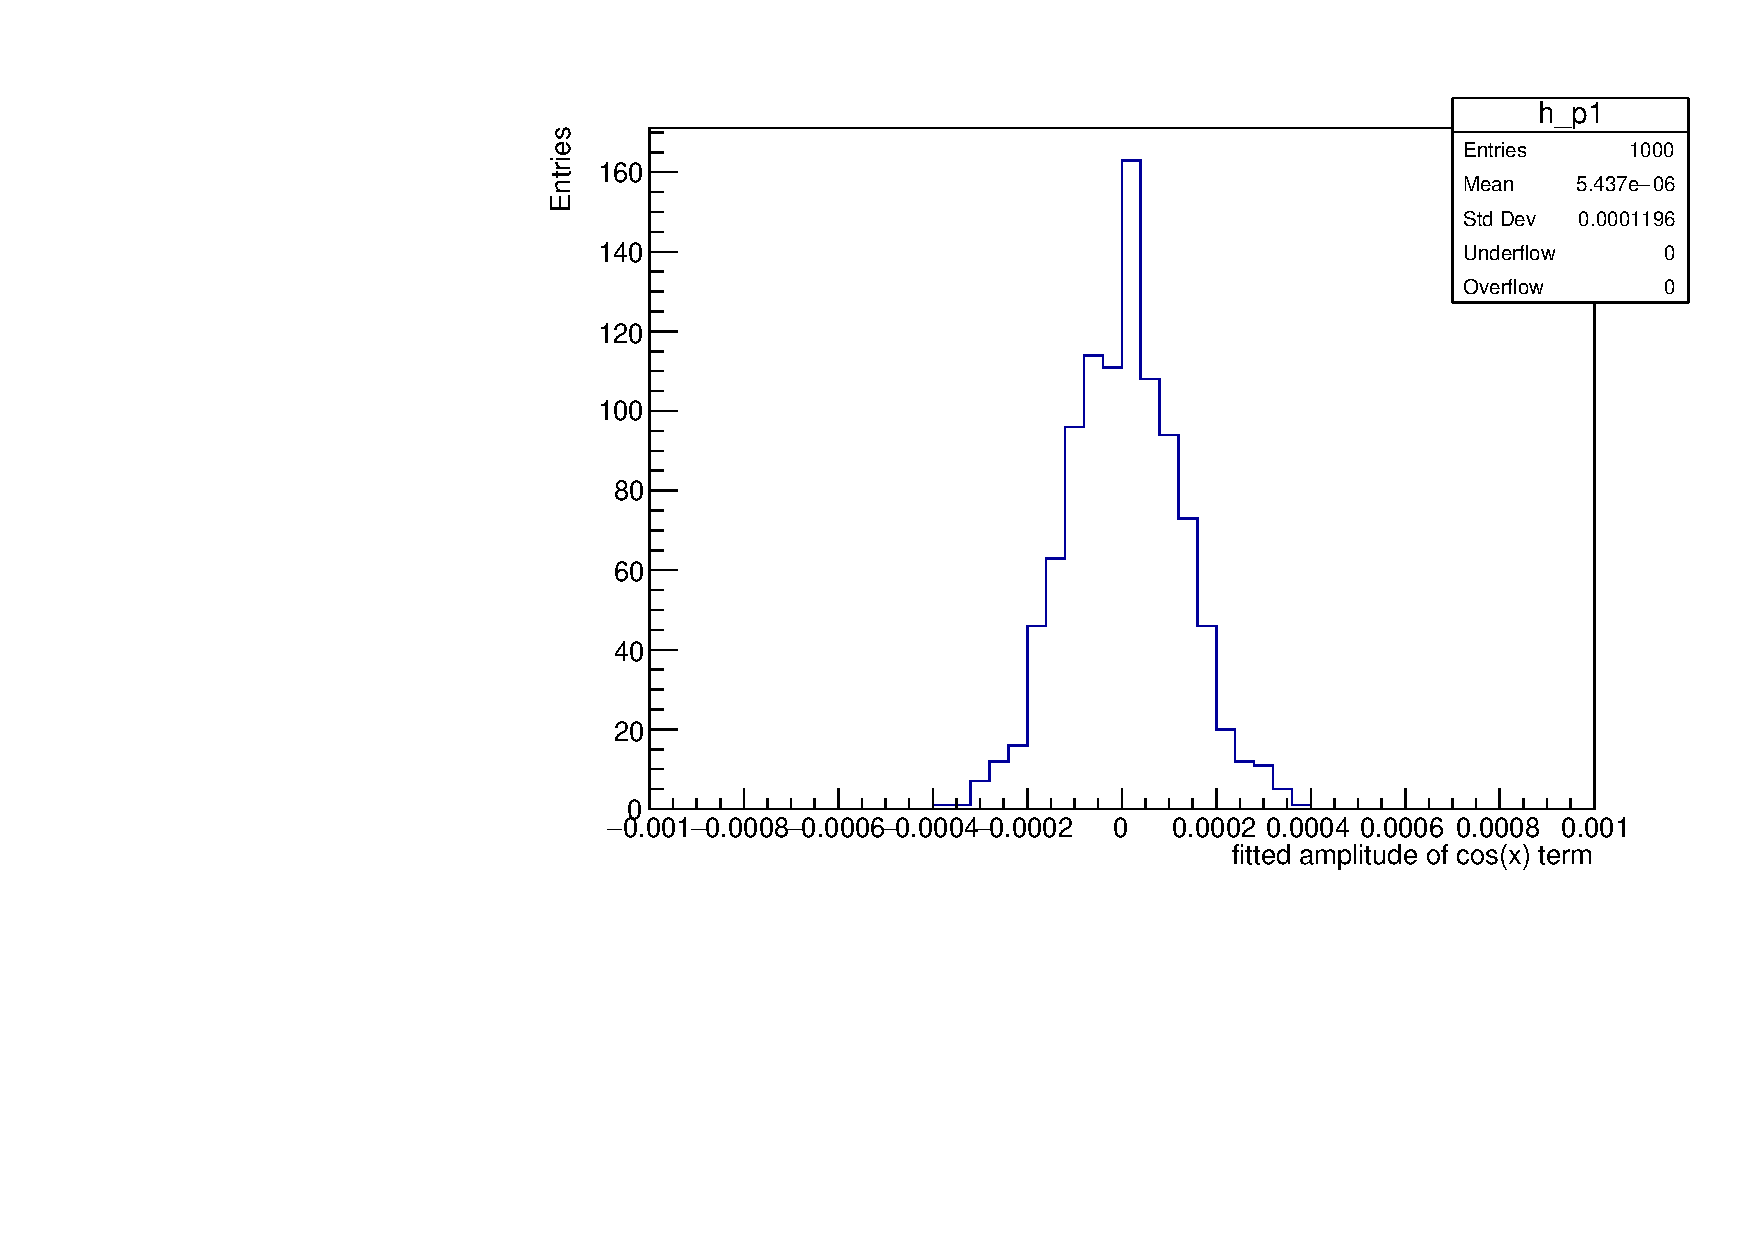
\includegraphics[width=0.4\textwidth]{figs/toy/res_1000_toy_p1.pdf}
\caption{\label{fig:toy_1000exp_s1pb} Result of 1000 toy experiement with LIV signal amplitude of 1 pb. Fit function is 1 + p0 sin(x)+p1 cos(x). 
(left) amplitude of sin(x) term, (right) amplitude of cos(x). }
\end{figure}

Figure~\ref{fig:toy_1000exp_s03pb} shows same set of result close to 3 sigma level sensitivity (only taken into account statistics uncertainty). 
The injected signal amplitude is 300 fb.

\begin{figure}
\centering
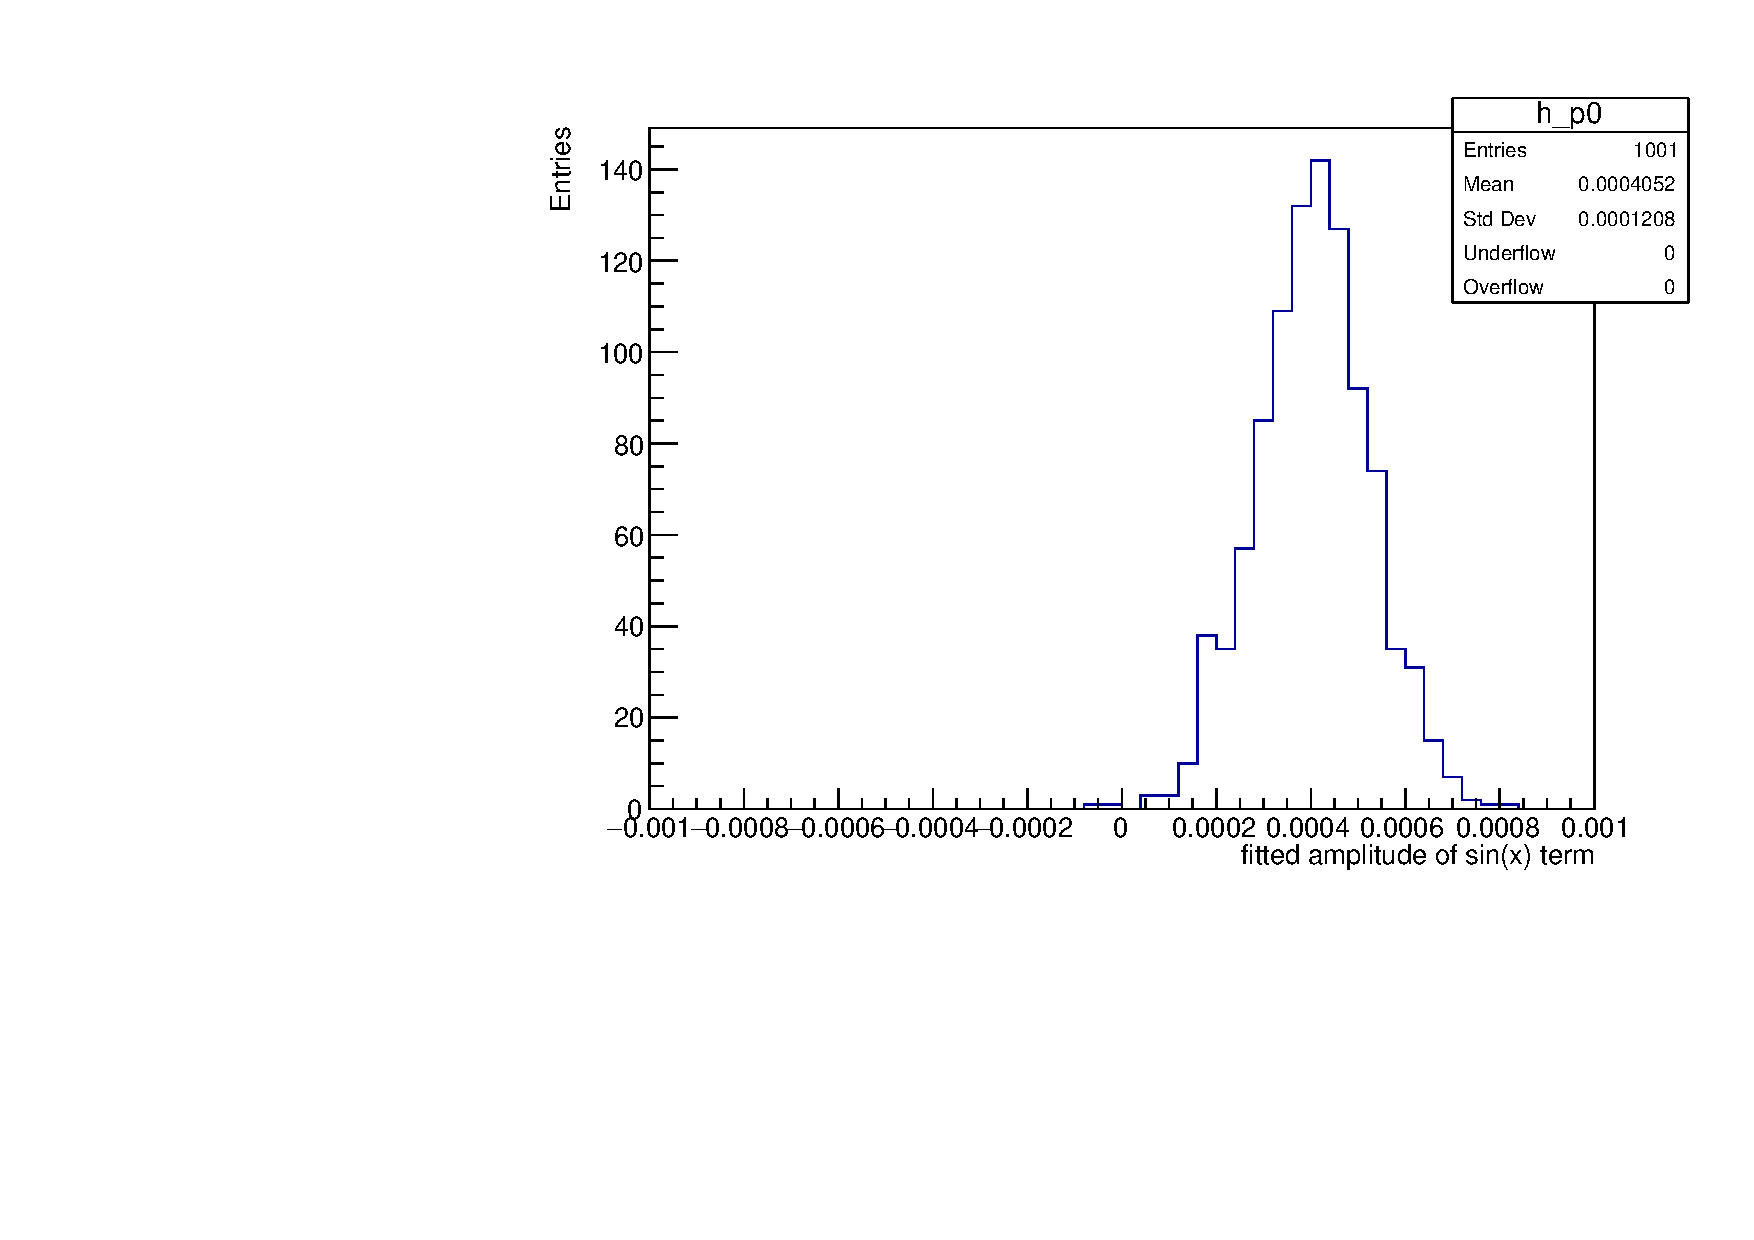
\includegraphics[width=0.4\textwidth]{figs/toy/res_1000_toy_sig0p3_p0.pdf}
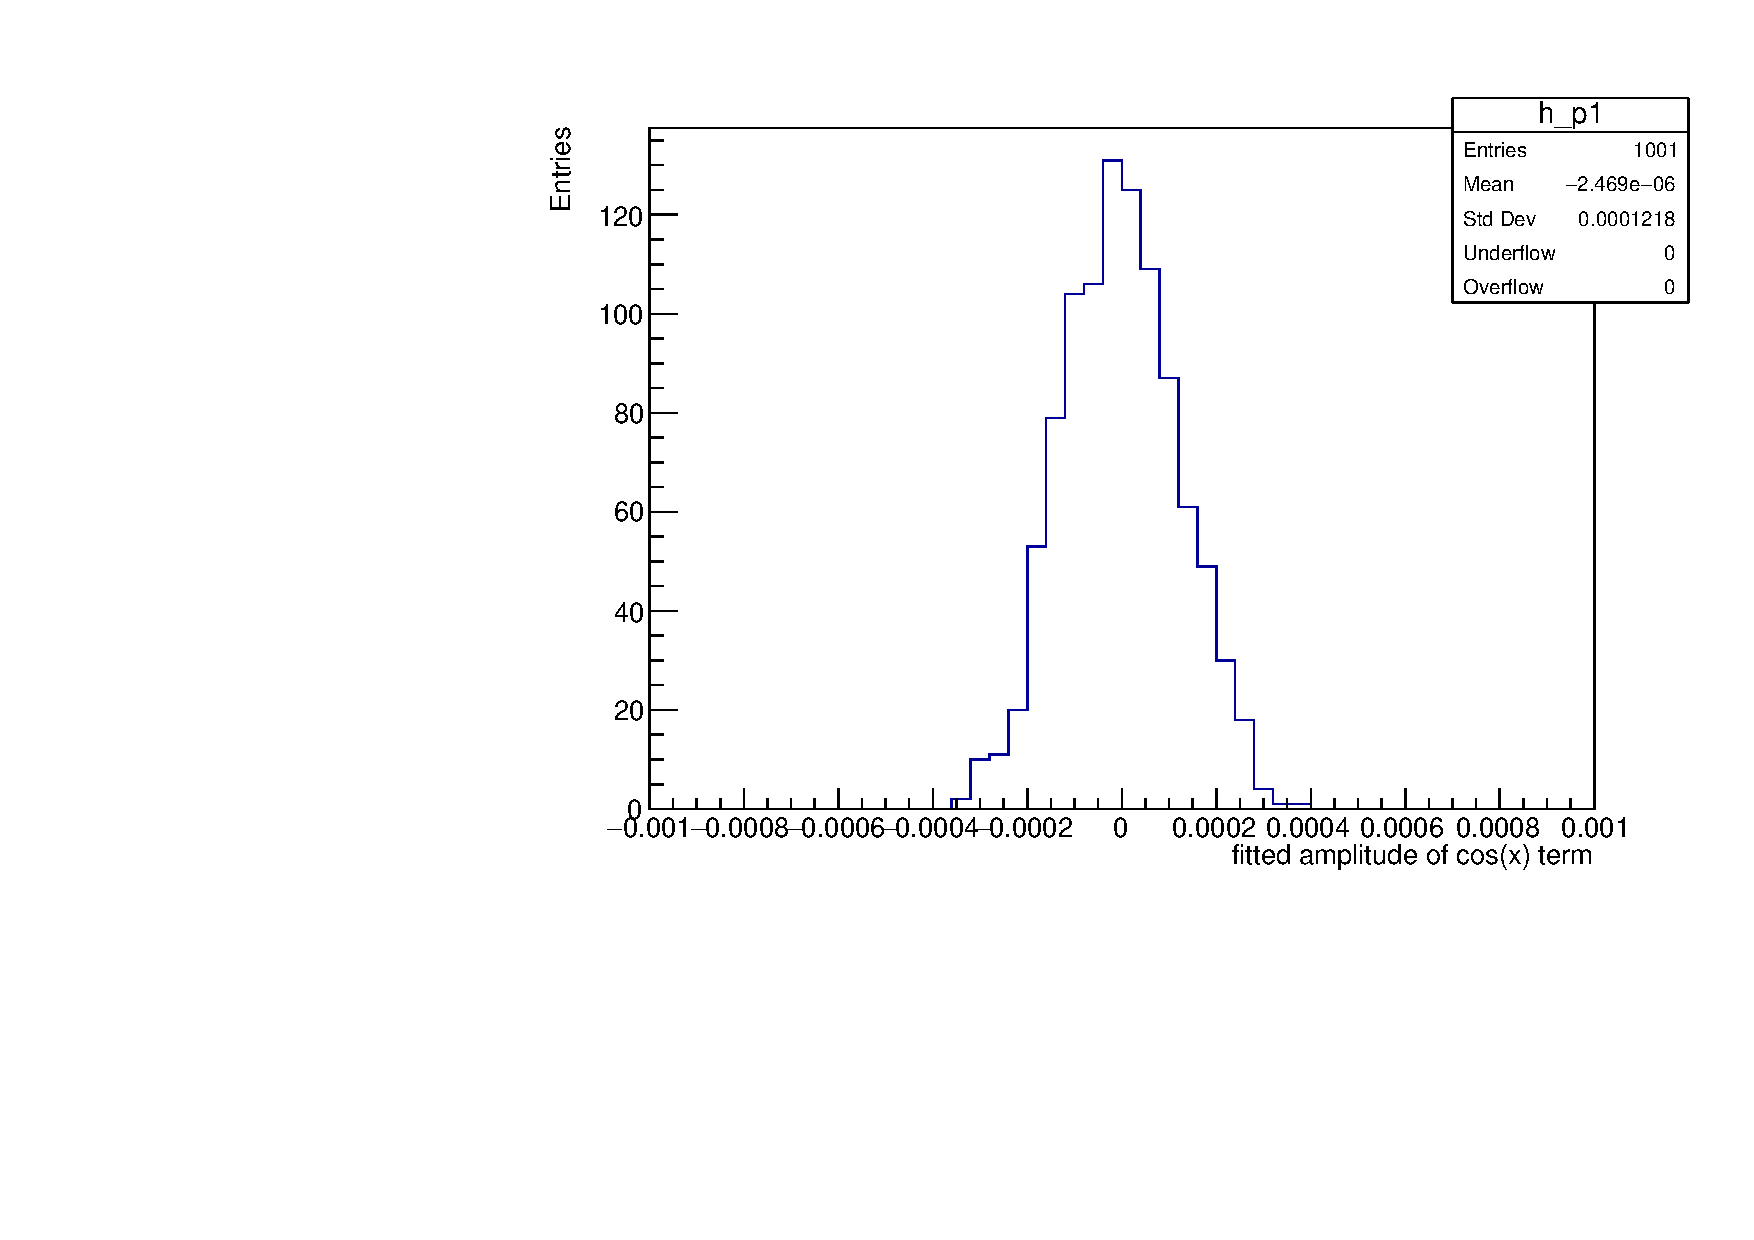
\includegraphics[width=0.4\textwidth]{figs/toy/res_1000_toy_sig0p3_p1.pdf}
\caption{\label{fig:toy_1000exp_s03pb} Result of 1000 toy experiement with LIV signal amplitude of 0.3 pb. Fit function is 1 + p0 sin(x)+p1 cos(x). 
(left) amplitude of sin(x) term, (right) amplitude of cos(x). }
\end{figure}


\subsubsection{Number of bin in sidereal phase}
\label{sec:number_of_bins}
 Number of binning in sidereal phase is scanned with simple Toy. Result is shown in Fig.~\ref{fig:toy_sig_nbins_liv_1pb}, 
which is performed with LIV signal amplitude of 1 pb. As expecdted, low number of bins shows low significance, 
this is just simply cancel negative part and positive part of signal due to coarse binning.
An interesting observation is there are small bias around number of bins from 10 to 15. It has higher than reaching plateau, after number of bins greater than 25. 
This indicates it's better to use enough large number of bins. For finer direction, the Run-2 data provides a large number of Z events, therefore we could use very fine binning. 
Finest limit case would be 1440, which is based on duration of LB (60 seconds) over 24 hours. 
To avoid too fine bin, we choose number of bins of 100 as the default configuration. Here 1 bin corresponds to about 15 min duration for the sidereal phase.

\begin{figure}
\centering
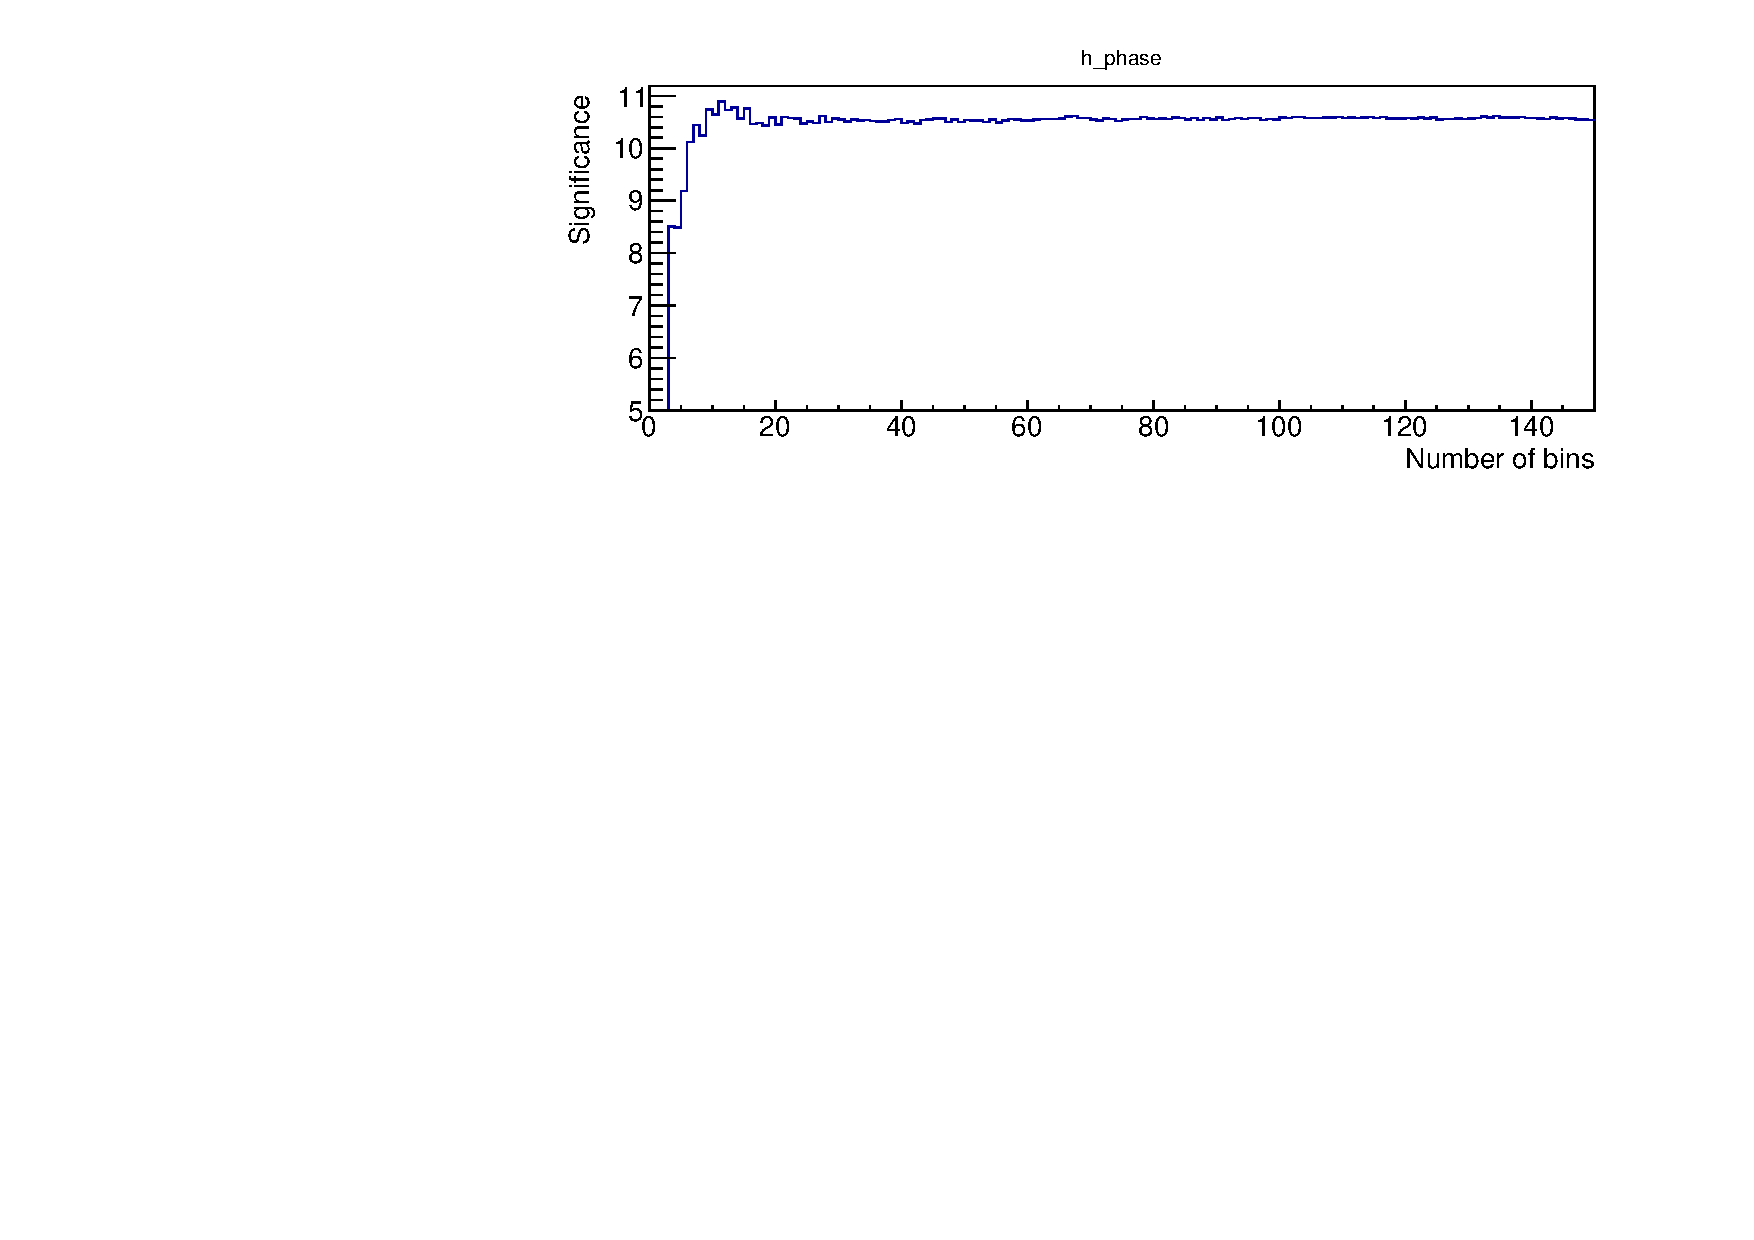
\includegraphics[width=0.8\textwidth]{figs/toy/sig_nbins_liv_1pb.pdf}
\caption{\label{fig:toy_sig_nbins_liv_1pb} Significance (quadrature sum of diviataion from 1 on the double ratio in sidereal 100 bins) as function of number of bins with no random case. Injected LIV amplitude is 1 pb. }
\end{figure}


\subsubsection{Changing probing sidereal period for expected signal}

 This study was made to check if we could check day-night effect. The difference of duration between solar day and the sidereal day is about 4 minutes, 
which corresponds to only $\sim 0.3$\%.  Looking the day-night effect may be effectively reveal the potential LIV effect. Fig.~\ref{fig:toy_sig_periodscale_zoom} 
confirms this hypothesis, we would see LIV signal with probing period with the solar day. In this test, inject signal amplitude is 1 pb sin curve with sidereal phase. 
And the significance is computed by changing the probing period scale factor, $\alpha_{preriod}$. Here the $\alpha_{preriod}$ is 
the scale factor on the period to compute phase. To have the period of solar day, $\alpha_{preriod}$ is 1.00274.  
In the figure, $\alpha_{preriod}$ is scanned from 0.975 to 1.025. Observed periodic peak structure.  Wider range of scan is shown in Fig.~\ref{fig:toy_sig_periodscale}. 

Base on this study, we understood we should not look the double ratio with the period of solar day in order to make blind data analysis.
We are planning to make step by step unblinding. Once all studies are performed, start to make fit on the double ratio with the probing phase of 1 hour and 7 hours.
%% More description on blinding strategy are discussed in Section.~\ref{sec:step_by_step_unblind_test}.
 
\begin{figure}
\centering
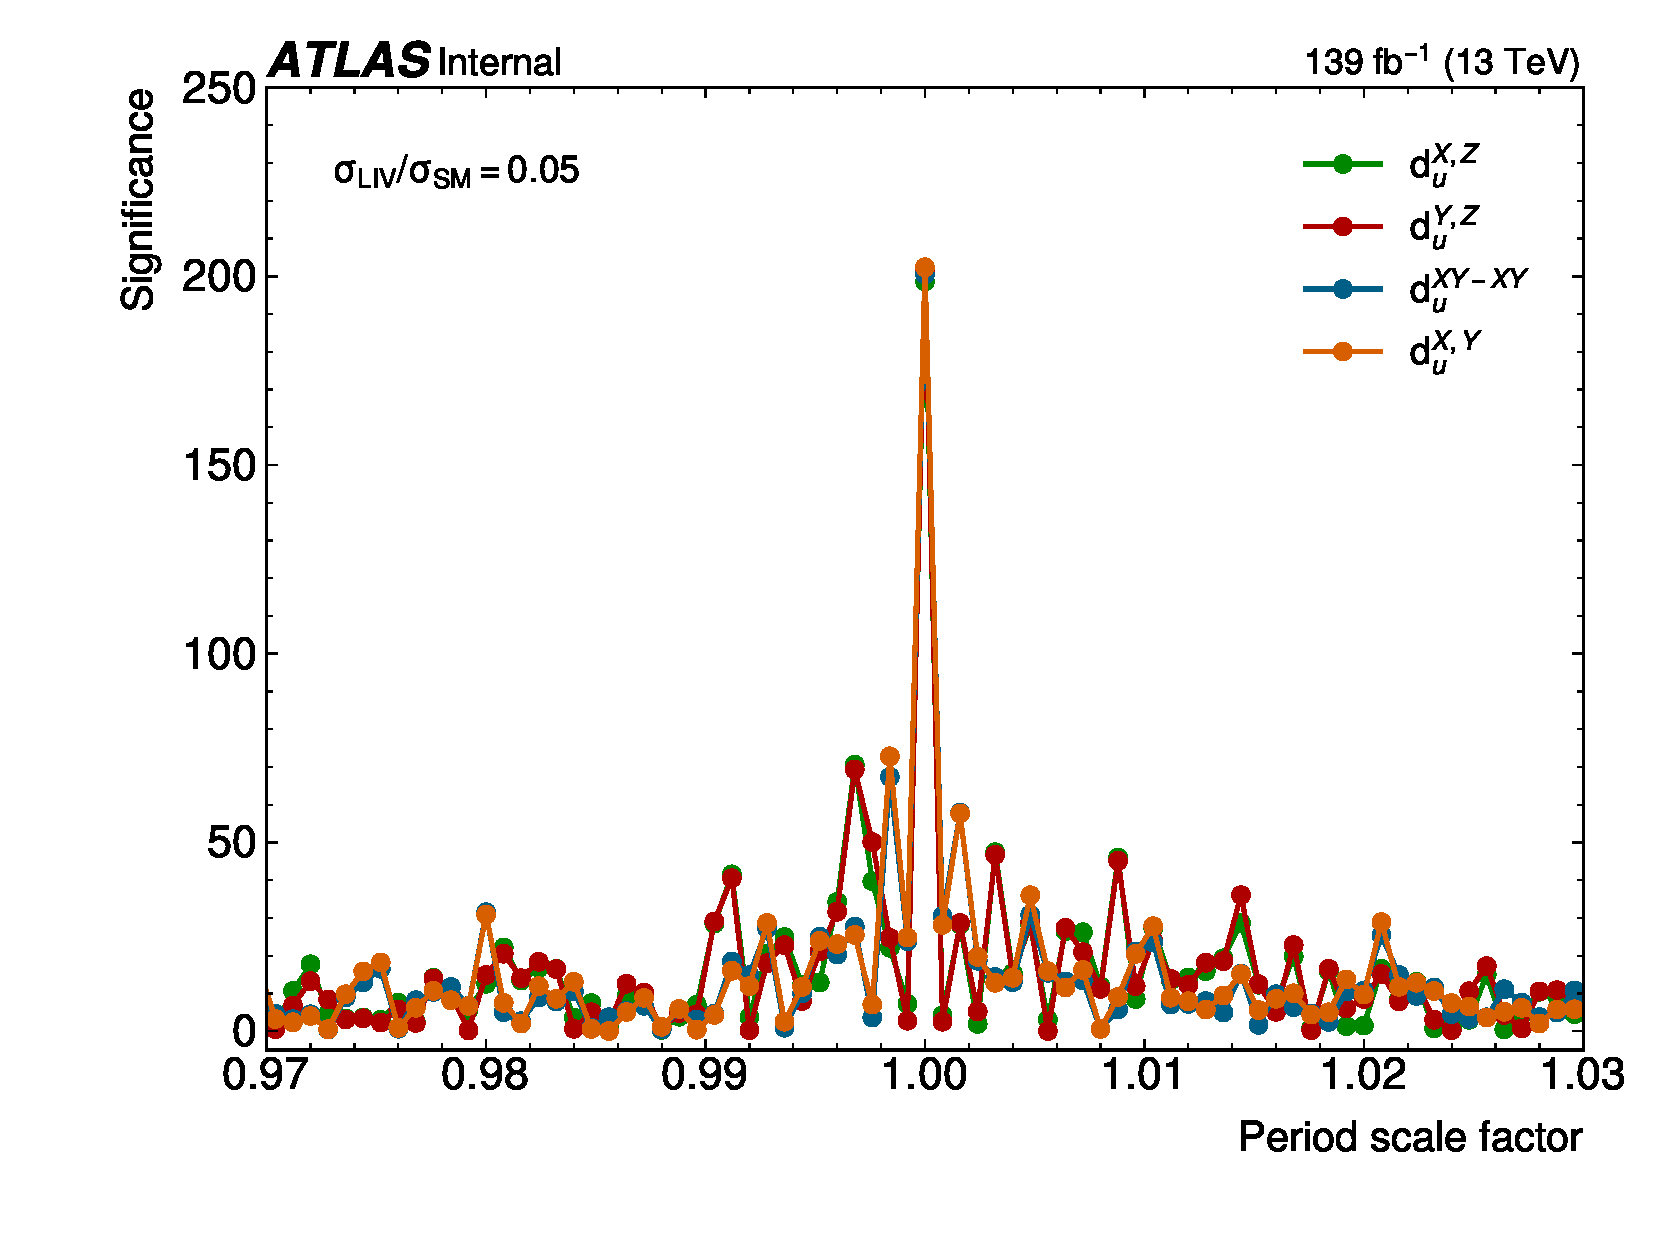
\includegraphics[width=0.6\textwidth]{figs/toy/sig_periodscale_zoom.pdf}
\caption{\label{fig:toy_sig_periodscale_zoom} Significance (quadrature sum of deviataion from 1 on the double ratio in sidereal 100 bins) as function of 
probing period scale factor with no random case. Injected LIV amplitude is 1 pb.  The period with scale factor = 1 is the 23h56m04s, which is used to generate signal.  { TO BE UPDATED with figure from Ablet} }
\end{figure}


\begin{figure}
\centering
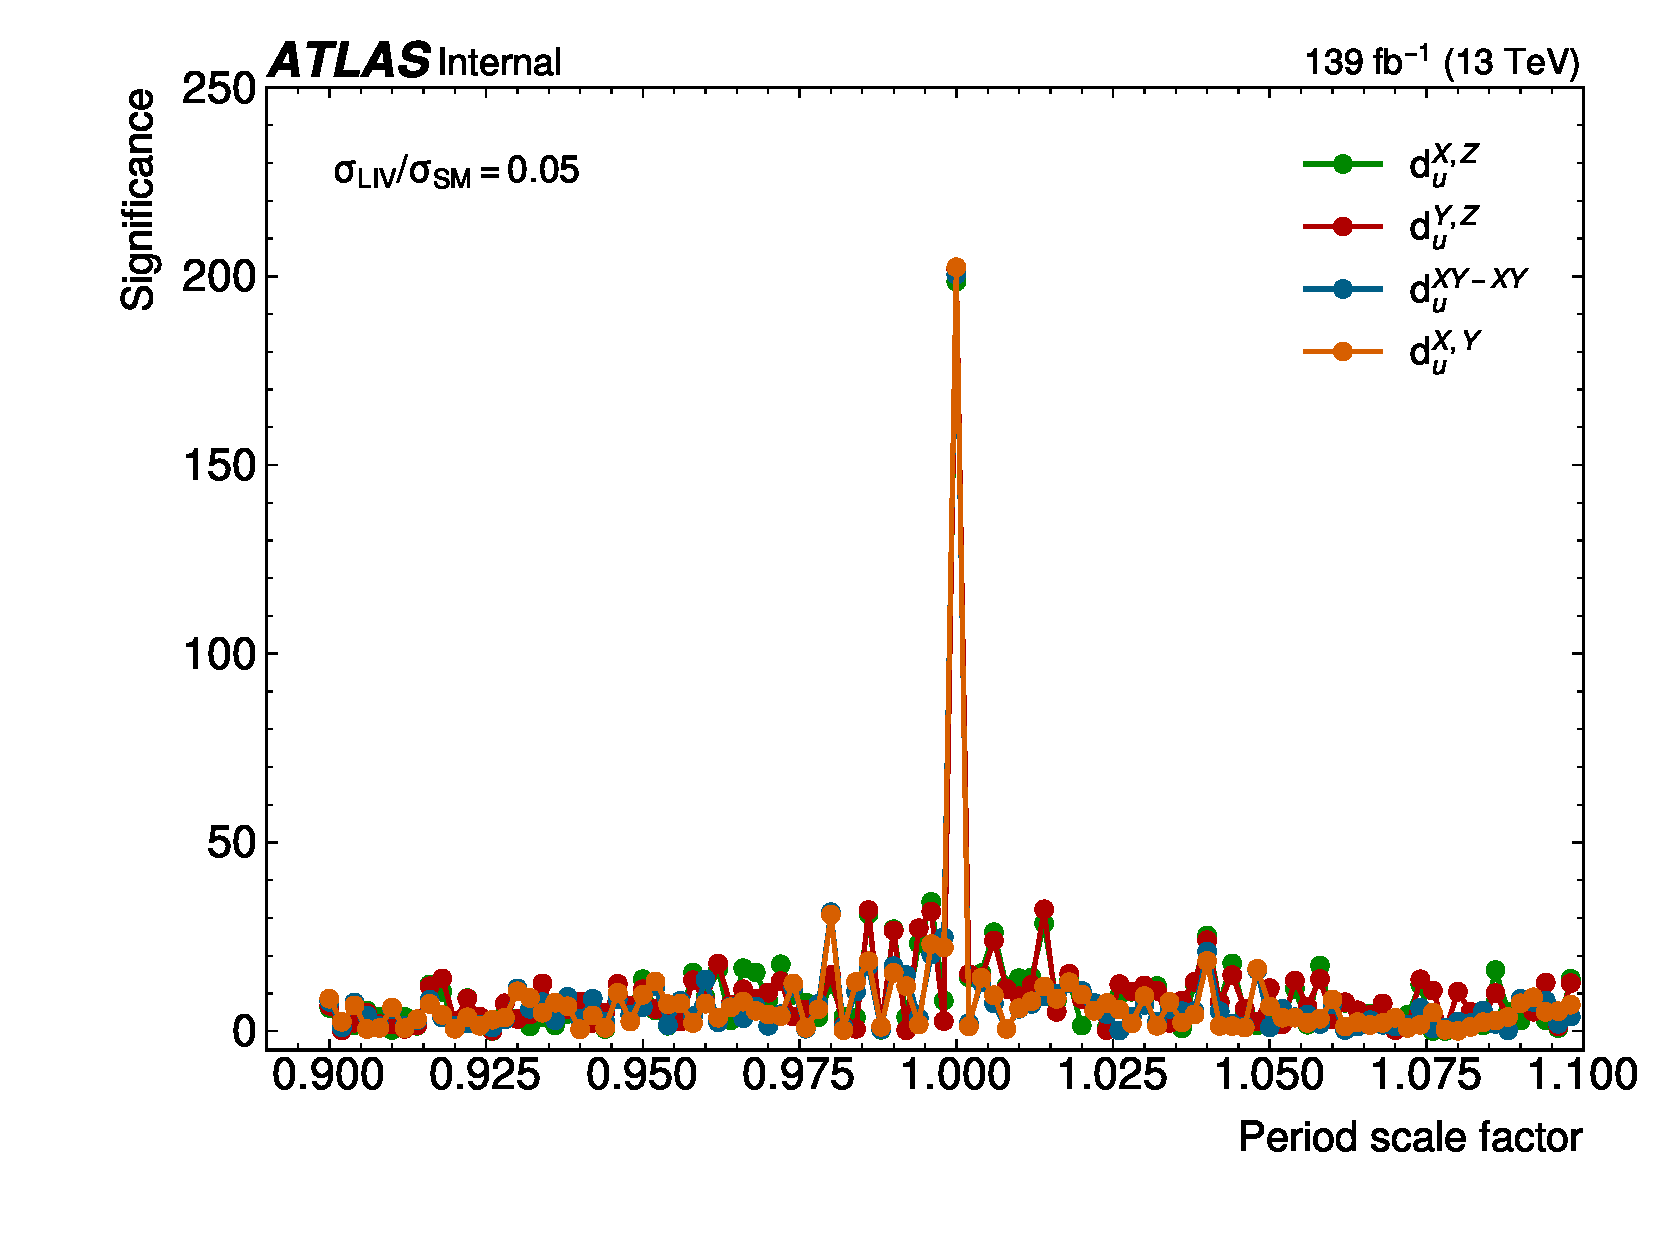
\includegraphics[width=0.6\textwidth]{figs/toy/sig_periodscale2.pdf}
\caption{\label{fig:toy_sig_periodscale} Significance as function of probing period scale factor with no random case. Injected LIV amplitude is 1 pb.  
The period with scale factor = 1 is the 23h56m04s, which is used to generate siganl. { TO BE UPDATED with figure from Ablet}}
\end{figure}
%% \subsubsection{blind TOY study}


\subsubsection{Study on the effect of correction}

 Effect of efficieincy correction is checked also simple TOY study.
Above studies are all not taken into account efficiency effect on the Z counting method. As described in Section~\ref{lab:Methodology},
there are $<\mu>$ dependent efficiency changes, i.e. on lepton reconstruction and trigger. These effects are modeled in Toy generation.
Electron efficiency is parameterized as a function of $<mu>$, and generated Toy based on it. 
Figure~\ref{fig:toy_effect_efficiency}(left) shows the double ratio with NULL signal configuration without applying the efficiency effect. 
The double ratio shows a flat dependence. Once efficiency effect taken into accout as the middle figure of Fig.~\ref{fig:toy_effect_efficiency}, 
structure showing up. This is because profile of $<mu>$ as function of sidereal phase is not flat due to limited statistics. 
This is small effect, but it become large effect on the double ratio. 

 Figure ~\ref{fig:toy_effect_efficiency}(right) shows same one after applying efficiency correction. In case the modeling of efficiency dependence is well understood,
we can minimize the modulation due to $<mu>$ dependent modulation on the double ratio. 
This could be the largest systematic uncertainty of the search.

\begin{figure}
\centering
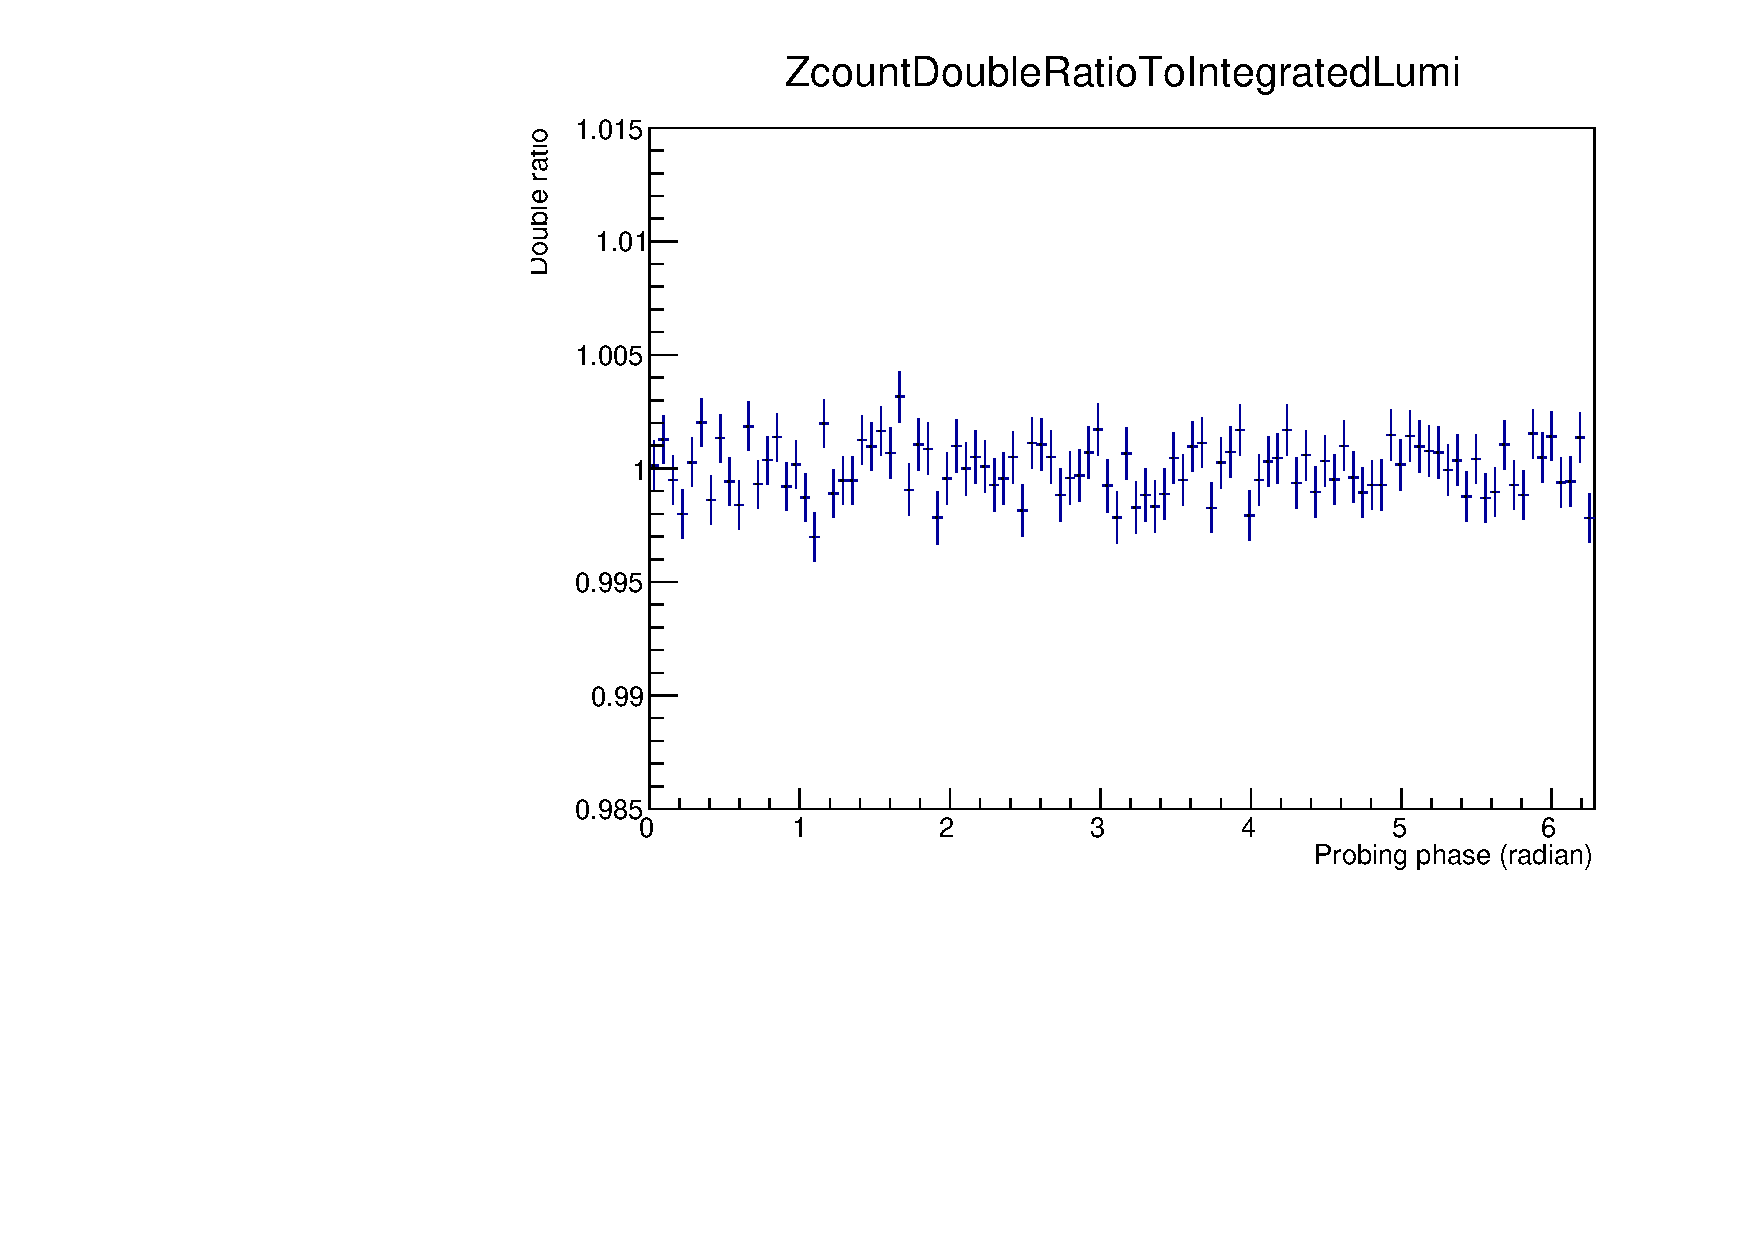
\includegraphics[width=0.33\textwidth]{figs/toy/fig_bin100_LIVxsec_0_random1_period1000_probe24_SigConfig0_LumiProf1_full_ZcountDoubleRatioToIntegratedLumi.pdf}
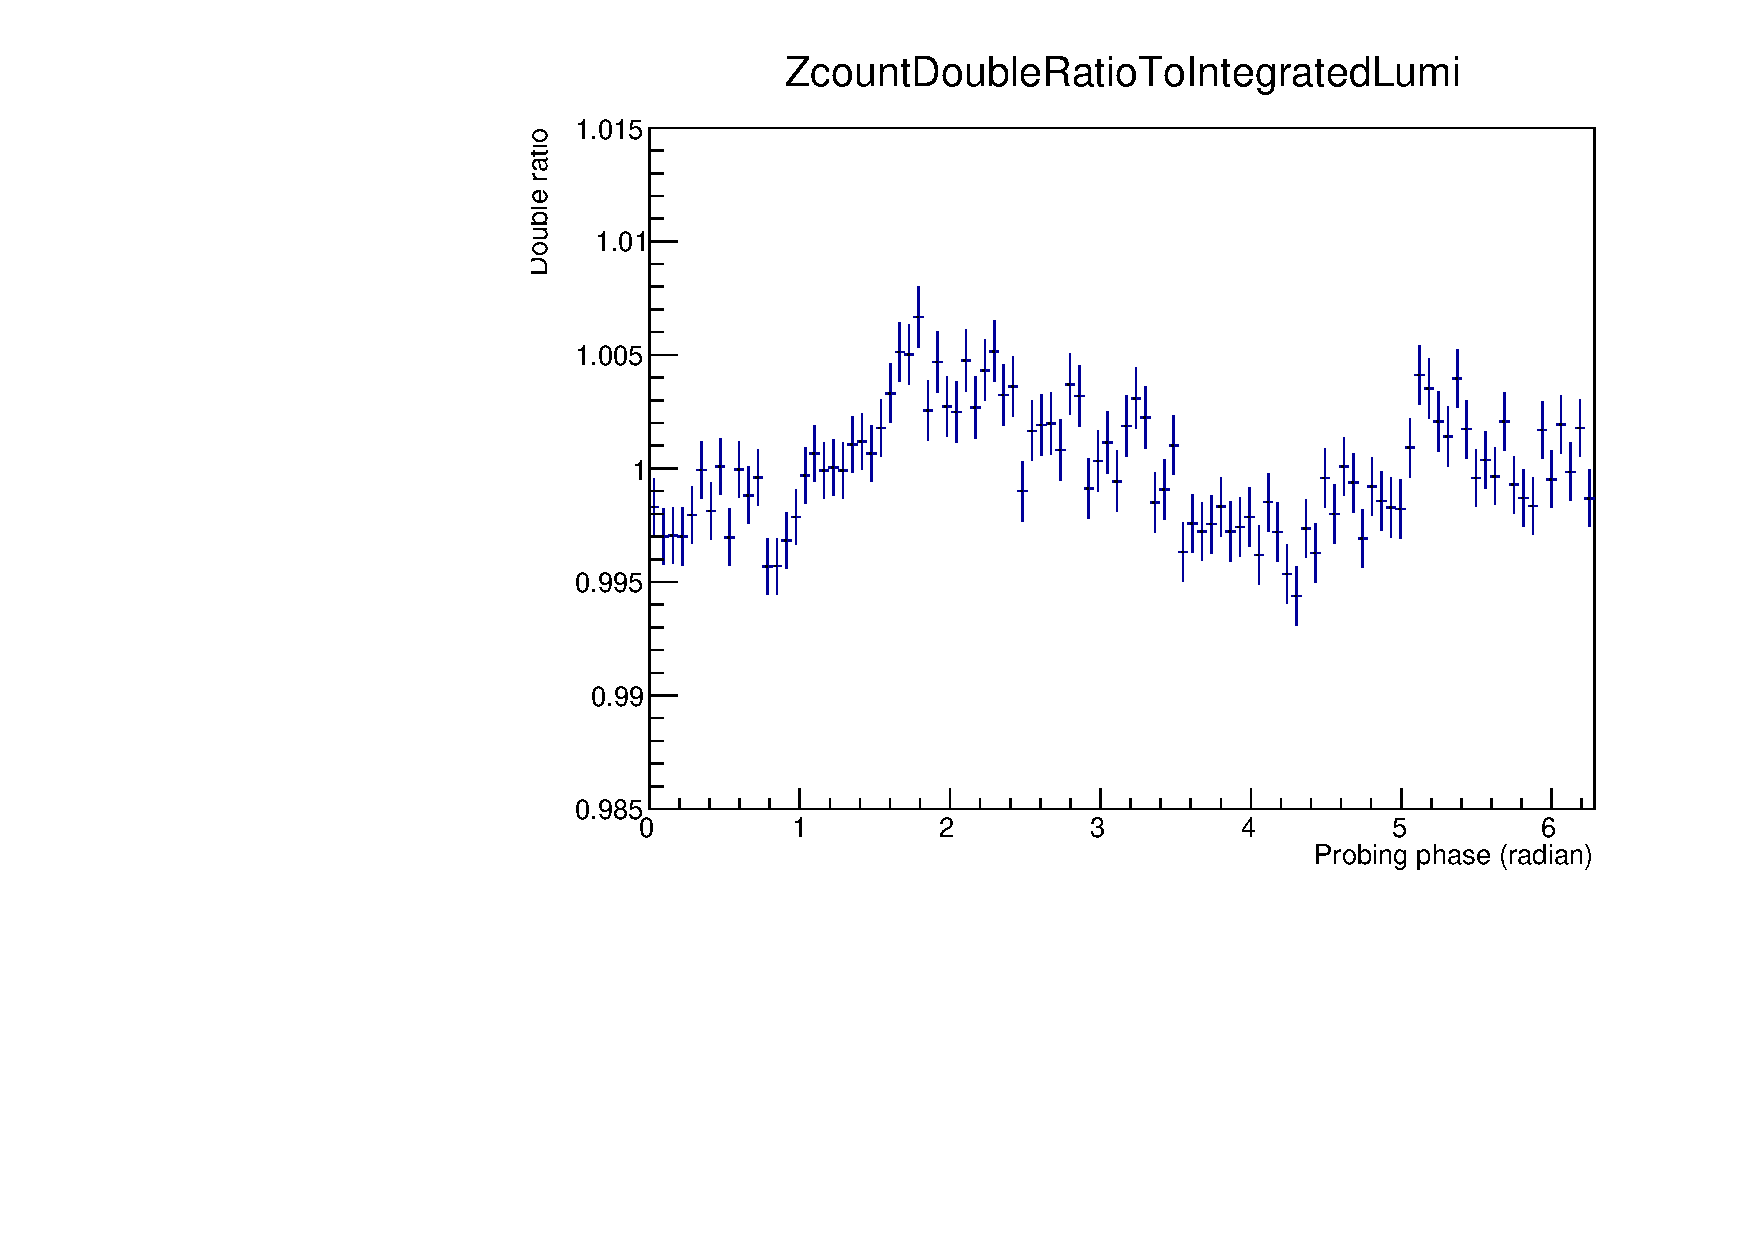
\includegraphics[width=0.33\textwidth]{figs/toy/fig_bin100_LIVxsec_0_random1_period1000_probe24_SigConfig101_LumiProf1_full_ZcountDoubleRatioToIntegratedLumi.pdf}
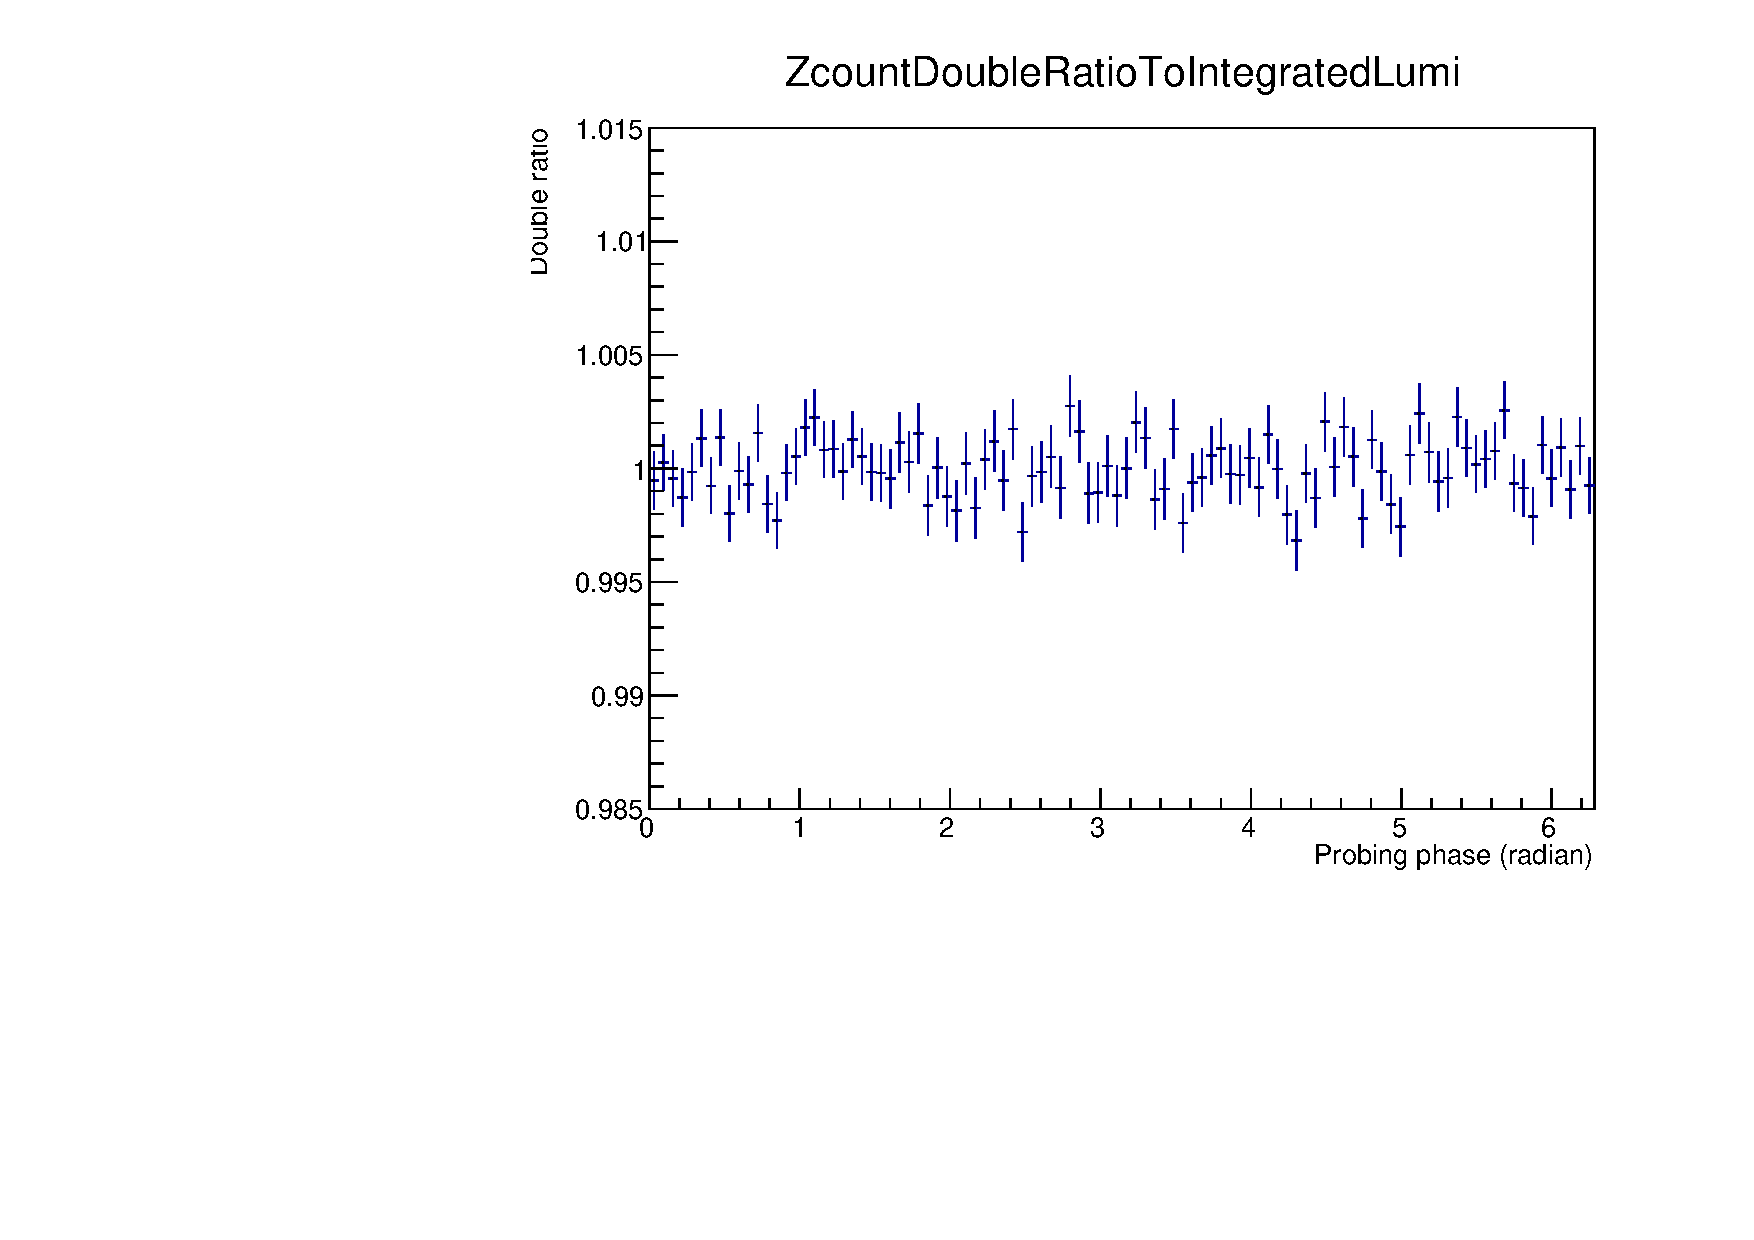
\includegraphics[width=0.33\textwidth]{figs/toy/fig_bin100_LIVxsec_0_random1_period1000_probe24_SigConfig201_LumiProf1_full_ZcountDoubleRatioToIntegratedLumi.pdf}
\caption{\label{fig:toy_effect_efficiency} Effect of efficiency correction and its correction to the double ratio. Left: The double ratio in case efficiency=1, Middle: The double ratio with efficiency effect taken into account, Right: the double ratio with efficiency effect after applying its correction. These are generated with NULL signal configuration.}
\end{figure}


\subsubsection{One run behavior with TOY experiment}
 During ATLAS data taking, we are monitoring various physics observables. Number of Z is also one of observable. 
In case a large LIV effect, we would see large effect on number of Z as function of sidereal time. 
For example, Fig.~\ref{fig:toy_large_signal} shows case of $d_u^{XY} \sim 10^{-3}$, the amplitude in the double ratio would be larger than 15\%. 
This level, we would notice during data taking or data quality check. 

\begin{figure}
\centering
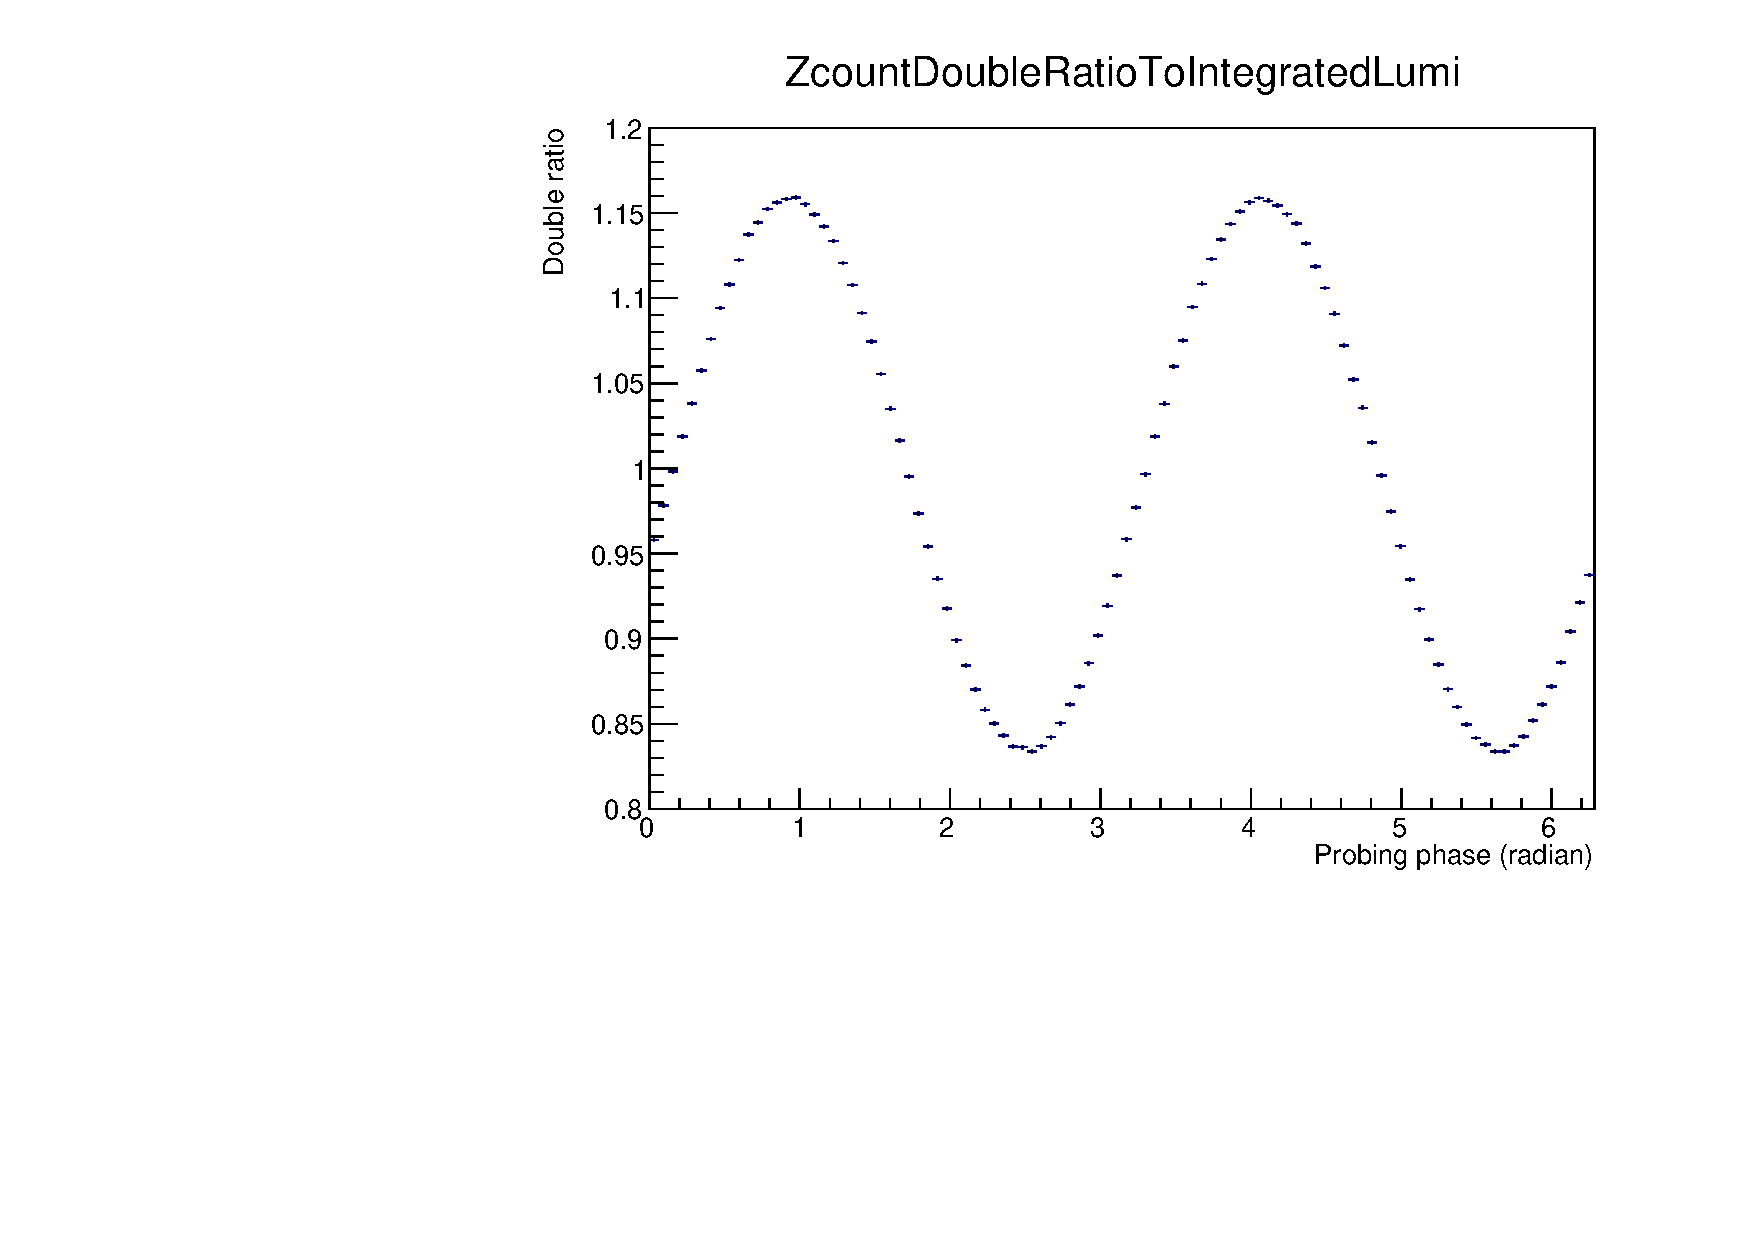
\includegraphics[width=0.4\textwidth]{figs/toy/fig_bin100_LIVxsec_577_random1_period1000_probe24_SigConfig29_LumiProf1_full_ZcountDoubleRatioToIntegratedLumi.pdf}
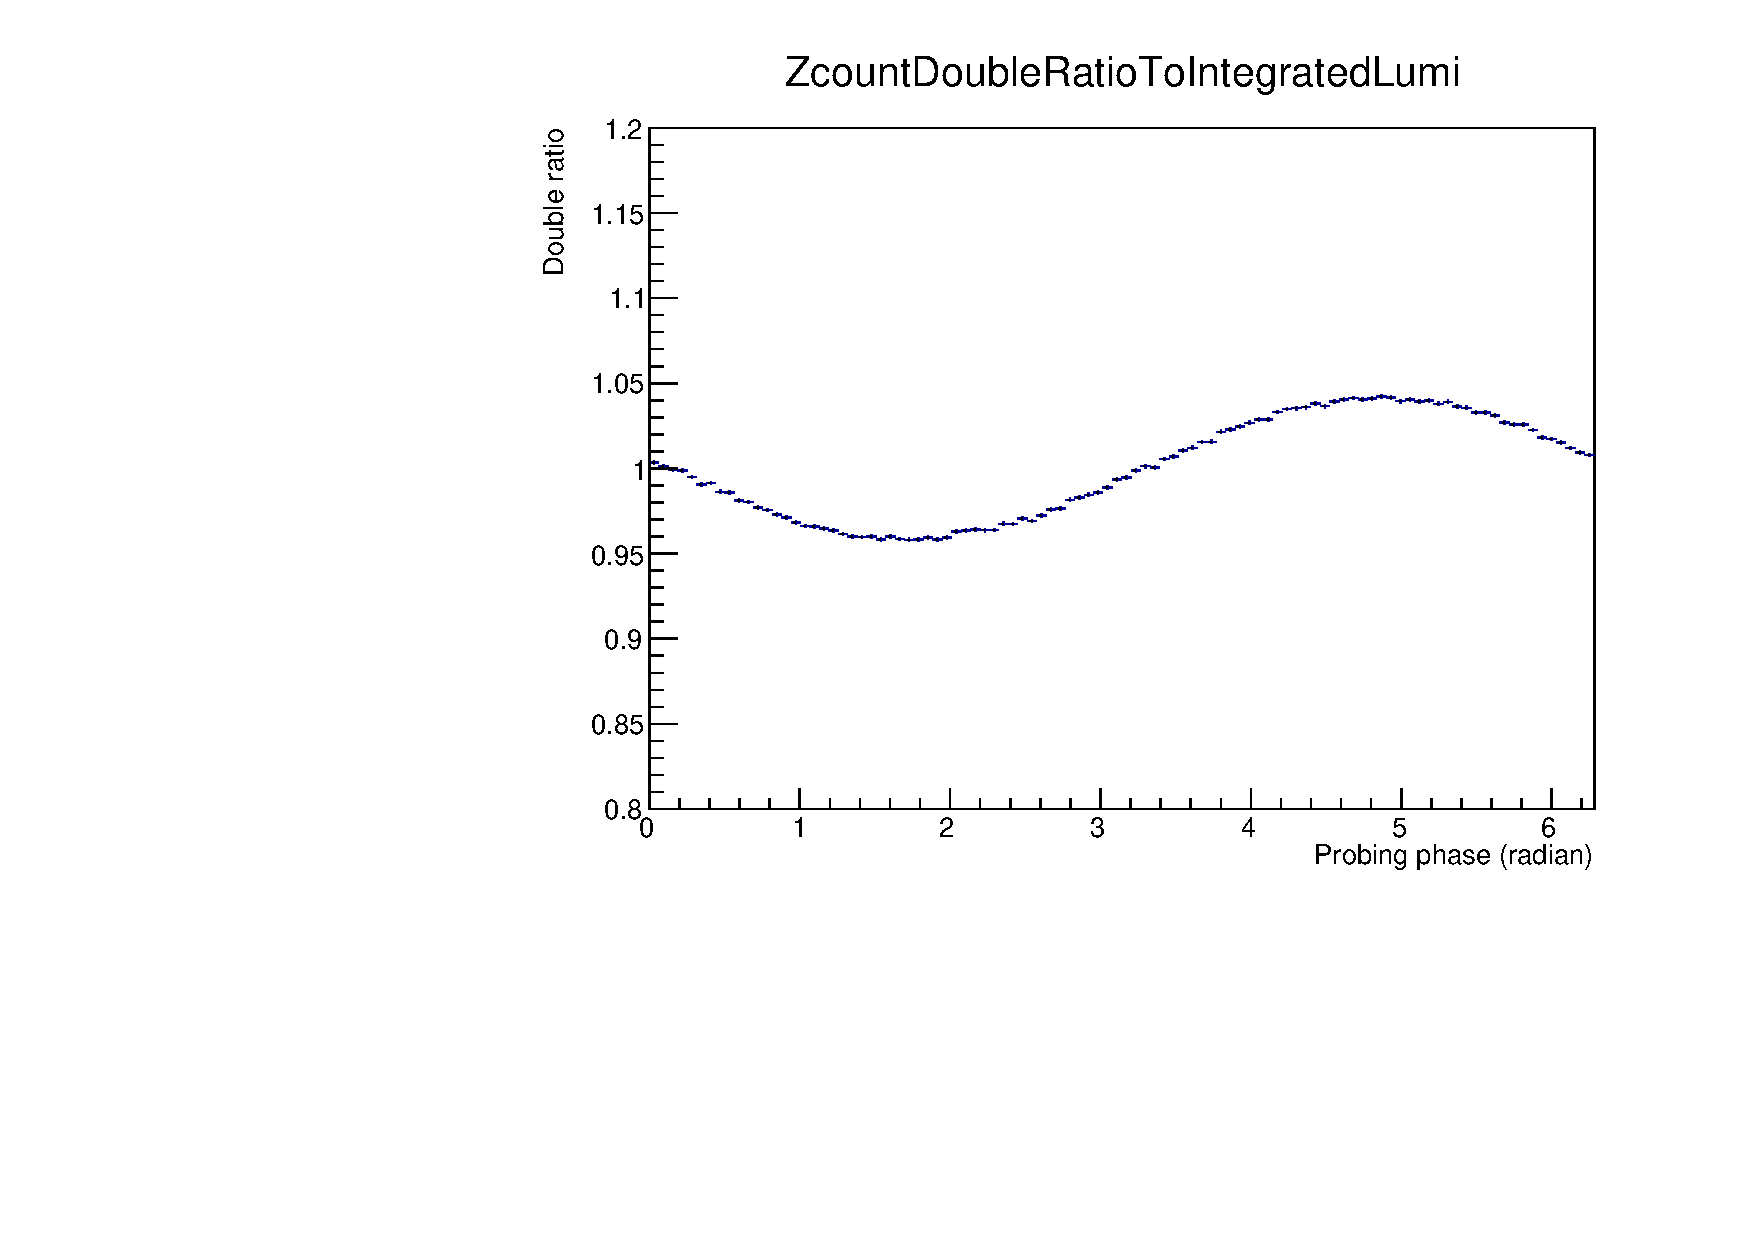
\includegraphics[width=0.4\textwidth]{figs/toy/fig_bin100_LIVxsec_577_random1_period1000_probe24_SigConfig26_LumiProf1_full_ZcountDoubleRatioToIntegratedLumi.pdf}
\caption{\label{fig:toy_large_sig_run340030} Expected double ration for the case of $d_u^{XY} = 10^{-3}$ (left) and $d_u^{YZ} = 10^{-3}$ (right). Very large oscillation would be observed.}
\end{figure}

Figure~\ref{fig:toy_large_sig_run340030} shows the expected double ratio with $d_u^{YZ} = 10^{-3}$ in the longest run in 2017 data taking. With this level of signal, 
just one run of data would be enough to notice. We consider that amplitudes larger than a few \% are already excluded. 

Relation between significance and signal strength (ratio of the amplitude of LIV effect and SM Z yields) for wilson coeffiicnets shows in Fig.~\ref{fig:toy_signif_amplitude_d}.

Peak amplitude of the LIV effect, $(\sigma_{SME}-\sigma_{SM})/\sigma_{SM}$, with wilson coefficients are one are listed Table~\ref{tab:scan_range}. 
Scan ranges for each wilson coefficient are set at the peak amplitude at 5\% which are summarized in the same Table.


\begin{figure}
\centering
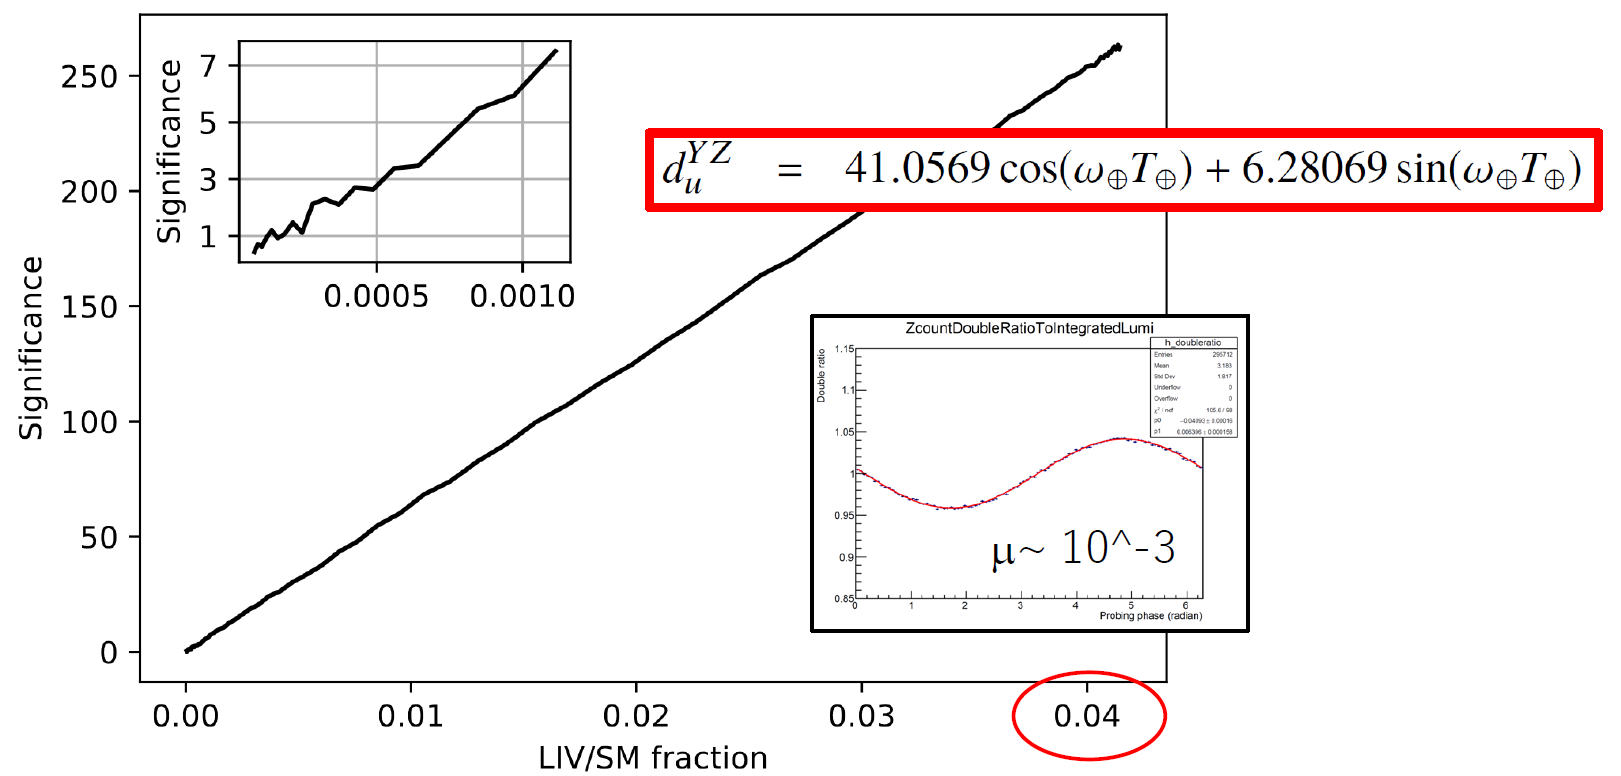
\includegraphics[width=0.43\textwidth]{figs/toy/Significance_Amplitude_for_d_YZ.png}
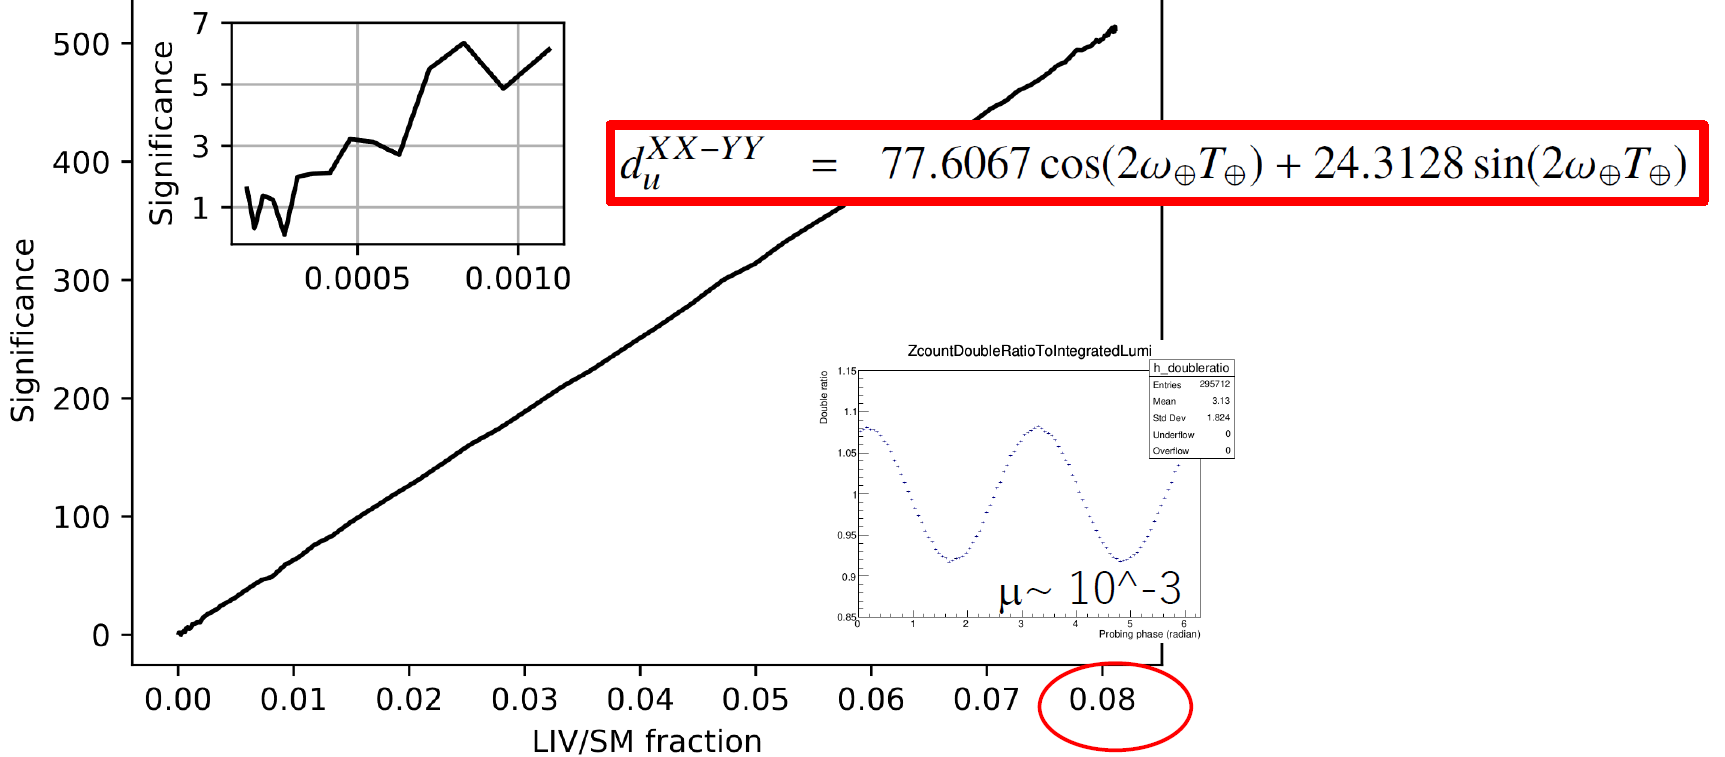
\includegraphics[width=0.46\textwidth]{figs/toy/Significance_Amplitude_for_d_XXYY.png}
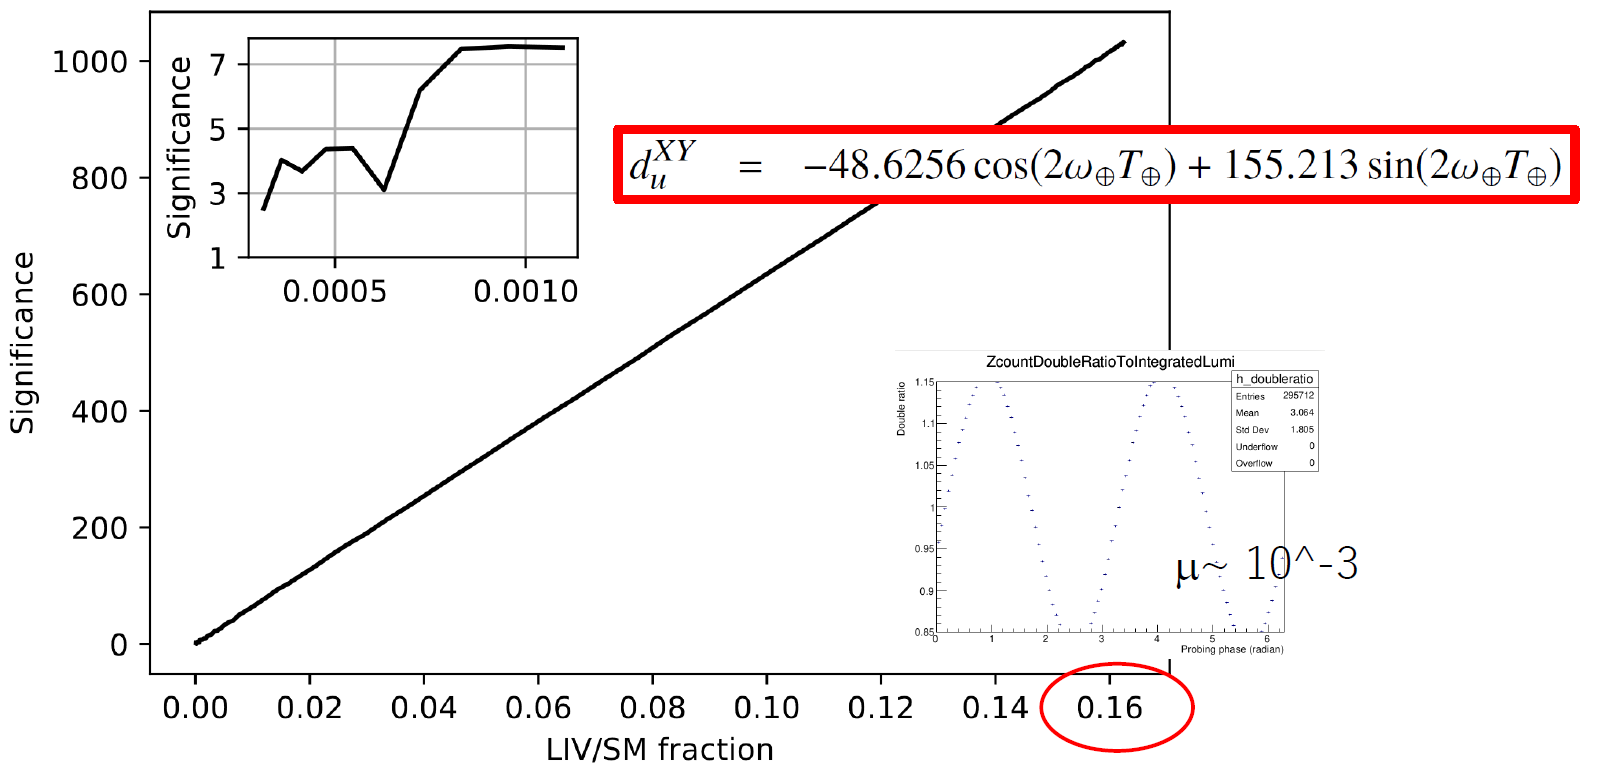
\includegraphics[width=0.43\textwidth]{figs/toy/Significance_Amplitude_for_d_XY.png}
\caption{\label{fig:toy_signif_amplitude_d} Significance as function of signal strangth for wilson coefficients $d_u^{YZ}$ (left), $d_u^{XX-YY}$ (middle) and $d_u^{XY}$ (right).}
\end{figure}



\begin{table}
\centering 
\begin{tabular}{c | c c} % centered columns (4 columns)
Coefficient & peak amplitude & upper bound (peak amplide of  = 0.05)  \\
\hline
%%   $d_u^{XZ}    $ & x.xx $ \times 10^{-z}$  \\
%%   $d_u^{YZ}    $ & x.xx $ \times 10^{-z}$  \\
%%   $d_u^{XX-YY} $ & x.xx $ \times 10^{-z}$  \\
%%   $d_u^{XY}    $ & x.xx $ \times 10^{-z}$  \\
%%   $c_u^{XZ}    $ & x.xx $ \times 10^{-z}$  \\
%%   $c_u^{YZ}    $ & x.xx $ \times 10^{-z}$  \\
%%   $c_u^{XX-YY} $ & x.xx $ \times 10^{-z}$  \\
%%   $c_u^{XY}    $ & x.xx $ \times 10^{-z}$  \\
%%   $c_d^{XZ}    $ & x.xx $ \times 10^{-z}$  \\
%%   $c_d^{YZ}    $ & x.xx $ \times 10^{-z}$  \\
%%   $c_d^{XX-YY} $ & x.xx $ \times 10^{-z}$  \\
%%   $c_d^{XY}    $ & x.xx $ \times 10^{-z}$  \\

 $d_u^{XZ}    $ & 41.53449  & 1.203819 $ \times 10^{-3}$ \\
 $d_u^{YZ}    $ & 41.53449  & 1.203819 $ \times 10^{-3}$ \\
 $d_u^{XX-YY} $ & 81.32592  & 6.148103 $ \times 10^{-4}$ \\
 $d_u^{XY}    $ & 162.6518  & 3.074048 $ \times 10^{-4}$ \\
 $c_u^{XZ}    $ & 53.45986  & 9.352805 $ \times 10^{-4}$ \\
 $c_u^{YZ}    $ & 53.45986  & 9.352805 $ \times 10^{-4}$ \\
 $c_u^{XX-YY} $ & 104.6762  & 4.776644 $ \times 10^{-4}$ \\
 $c_u^{XY}    $ & 209.3524  & 2.388322 $ \times 10^{-4}$ \\
 $c_d^{XZ}    $ & 1.200602  & 4.164584 $ \times 10^{-2}$ \\
 $c_d^{YZ}    $ & 1.200602  & 4.164584 $ \times 10^{-2}$ \\
 $c_d^{XX-YY} $ & 2.350819  & 2.126917 $ \times 10^{-2}$ \\
 $c_d^{XY}    $ & 4.701638  & 1.063459 $ \times 10^{-2}$  \\
\end{tabular}
\caption{\label{tab:scan_range} Peak amplitude of the LIV effect ($(\sigma_{SME}-\sigma_{SM})/\sigma_{SM}$) at each wilson coefficinet is 1, 
and their uppper bound of the scan range which are set at the amplitude of 5\%.}
\end{table}
  
  
  
  
  
  
  
  
  
  
  


\clearpage
\section{Data scrambling studies} %% [Ablet/Yuji/Enrico]
\label{lab:DataScrambling}
%\subsection{Methodology of data scrambling}
\label{lab:DataScrambling_method}

 In order to check data behavior with blinding on LIV effect, we have studied the data scrambling. 
This uses the measurement of Z counting for each LB in data. However, we do scrambling the time stamp. 
Because LIV effect can be probed by looking consequenced data, therefore if we scramble time stamp of each LB, 
we can not probe the LIV effect. 

 Actual method is very simple, we scramble time stamp of LBs within each year. No same time stamp is used twice. 
Actual function to scramble time stamps is the function, ''sample'', in random library of python3.

By using this dataset, we can check real value from the measurement with the lucid luminosity and the Z counting. 
In order to check staticial behavior, 1000 (or 10000) set of scrabled data are generated by using different seed in same way.
Number of LBs for each year of data is listed in Table.~\ref{tab:data_LBs}. 
Those are about 90 k LBs\footnote{we combine data15 and data16 because data15 has only 22 k LBs}, 
therefore we could generate different scriabled dataset by using different seed.

As we have three channels, electron, muon and combined, we check these output. 
  %% Yuji / Enrico
%% \input{sections/Sec_DataScrambling_2_Sample} %% Yuji
%%% \subsection{Statistical analyses}
\label{lab:DataScrambling_stat}

%% chi2 analysis.

The chi-squared ($\chi^{2}$) fit method is used to determine a signal strengh from a givent
 dataset (a double ratio). This method is commonly employed in various scientific 
 disciplines to assess how well a model describes the observed data.
 The formula for the chi-squared statistic is:
 \begin{equation}
    \chi^2 = \sum \frac{(O_i - E_i)^2}{\sigma_i^2},
 \end{equation}

 where 
 \begin{itemize}
    \item $i$ is the bin index, and it's range is [0-99] becuase we use 100 bins.
    \item $O_i$ is the observed value for data point $i$.
    \item $E_i$ is the expected value for data point $i$.
    \item $\sigma_i^2$ is the uncertainty (standard deviation) associated with the observed value.
 \end{itemize}

Datasets and theory models:
\begin{itemize}
    \item Dataset is a  double ratio obserable binned in a probing perioud.
     Total number of bin is 100 (see Section.~\ref{lab:ToyStudy}). The dataset is eigher toy, scrambled data or real data when
     this analysis is unblinded.
    
     \item Thery models are analytic fuctions predicted by SME theory described in 
     Section~\ref{lab:Theory}. Each model is fitted to a dataset independent to other models.
     and Each model has a free parameter, $\mu$, which is the signal strength.
    
    \item Degree of freedom: 100 bins minus number of free parameters which one in our case.
     So the DoF is 99.
\end{itemize}
 %% Ablet --> move to Section 3.
%\input{sections/Sec_DataScrambling_3_Results} %% Ablet
%\subsection{Increase number of scrambled datasets}
\label{lab:10K_scrambleddatasets}

%%%%%%%%%%%
%% Compare 1k and 10 results.
%% 1. create a table 
%% 2. Show plots

In this Section we comapred results across small and large sample sizes to study the  
impact of varying the number of scrambled datasets, 
as denoted by the sample size. We used two sample sizes, 1000 and 10000.
Table~\ref{table:scrambel_results_10K} shows fit results of two different sample size.
As we can see from the table that two set of results are consistent. Thus increasing number 
of scrambled datasets does not change results.

\begin{table}[hp]
    \begin{center}
    %%\resizebox{\textwidth}{!}{
    \begin{tabular}{|l|c|c|}
    \hline
    
    parameters & 1K & 10K \\ 
    \hline
    $d_{\it u}^{\it X,Z}$ & -2.98e-06 $\pm$ 3.68e-06& -2.99e-06 $\pm$ 3.62e-06\\
    \hline
    $d_{\it u}^{\it Y,Z}$ & -2.49e-06 $\pm$ 3.46e-06& -2.50e-06 $\pm$ 3.59e-06\\
    \hline
    $d_{\it u}^{\it XY,XY}$ & -1.62e-07 $\pm$ 1.86e-06& -2.39e-07 $\pm$ 1.89e-06\\
    \hline
    $d_{\it u}^{\it X,Y}$ & 1.05e-07 $\pm$ 9.27e-07& 1.41e-07 $\pm$ 9.40e-07\\
    \hline
    $c_{\it u}^{\it X,Z}$ & -2.31e-06 $\pm$ 2.86e-06& -2.32e-06 $\pm$ 2.81e-06\\
    \hline
    $c_{\it u}^{\it Y,Z}$ & -1.94e-06 $\pm$ 2.69e-06& -1.94e-06 $\pm$ 2.79e-06\\
    \hline
    $c_{\it u}^{\it XY,XY}$ & -1.26e-07 $\pm$ 1.45e-06& -1.86e-07 $\pm$ 1.47e-06\\
    \hline
    $c_{\it u}^{\it X,Y}$ & 8.17e-08 $\pm$ 7.20e-07& 1.09e-07 $\pm$ 7.31e-07\\
    \hline
    $c_{\it d}^{\it X,Z}$ & -1.03e-04 $\pm$ 1.27e-04& -1.03e-04 $\pm$ 1.25e-04\\
    \hline
    $c_{\it d}^{\it Y,Z}$ & -8.63e-05 $\pm$ 1.20e-04& -8.66e-05 $\pm$ 1.24e-04\\
    \hline
    $c_{\it d}^{\it XY,XY}$ & -5.59e-06 $\pm$ 6.45e-05& -8.27e-06 $\pm$ 6.54e-05\\
    \hline
    $c_{\it d}^{\it X,Y}$ & 3.64e-06 $\pm$ 3.21e-05& 4.86e-06 $\pm$ 3.25e-05\\
    \hline
    
    \hline
    \end{tabular}
    \end{center}
    \caption{Results from small and large number of scrambled datasets.
        Results are obtained using combined Run 2.
    }\label{table:scrambel_results_10K}
\end{table}







%%%%%%%%
%% Results of 10 batches
%%%%%%%%
%show ration table
To compete our studies, we split 10000 samples into 10 batches.
 Each batche contain 1000 scrabled datasets. In this study we comared
  results of 10 batches. Table of results of 10 batches
   is shown in the appendix~\ref{app:scrambled_10_batches}. 
The results in each batch is the average results obtained from 1000 fit results in
corresponding batch. Figure~\ref{fig:compare_10_batches} show the results 
 in each batch which is normalized to the result of first batch. The gray band in 
 the plot is the uncertainty band of the first batch. 
 From the plot we can see that results of 10 batches are consistent.

\begin{figure}[hp]
    \centering
    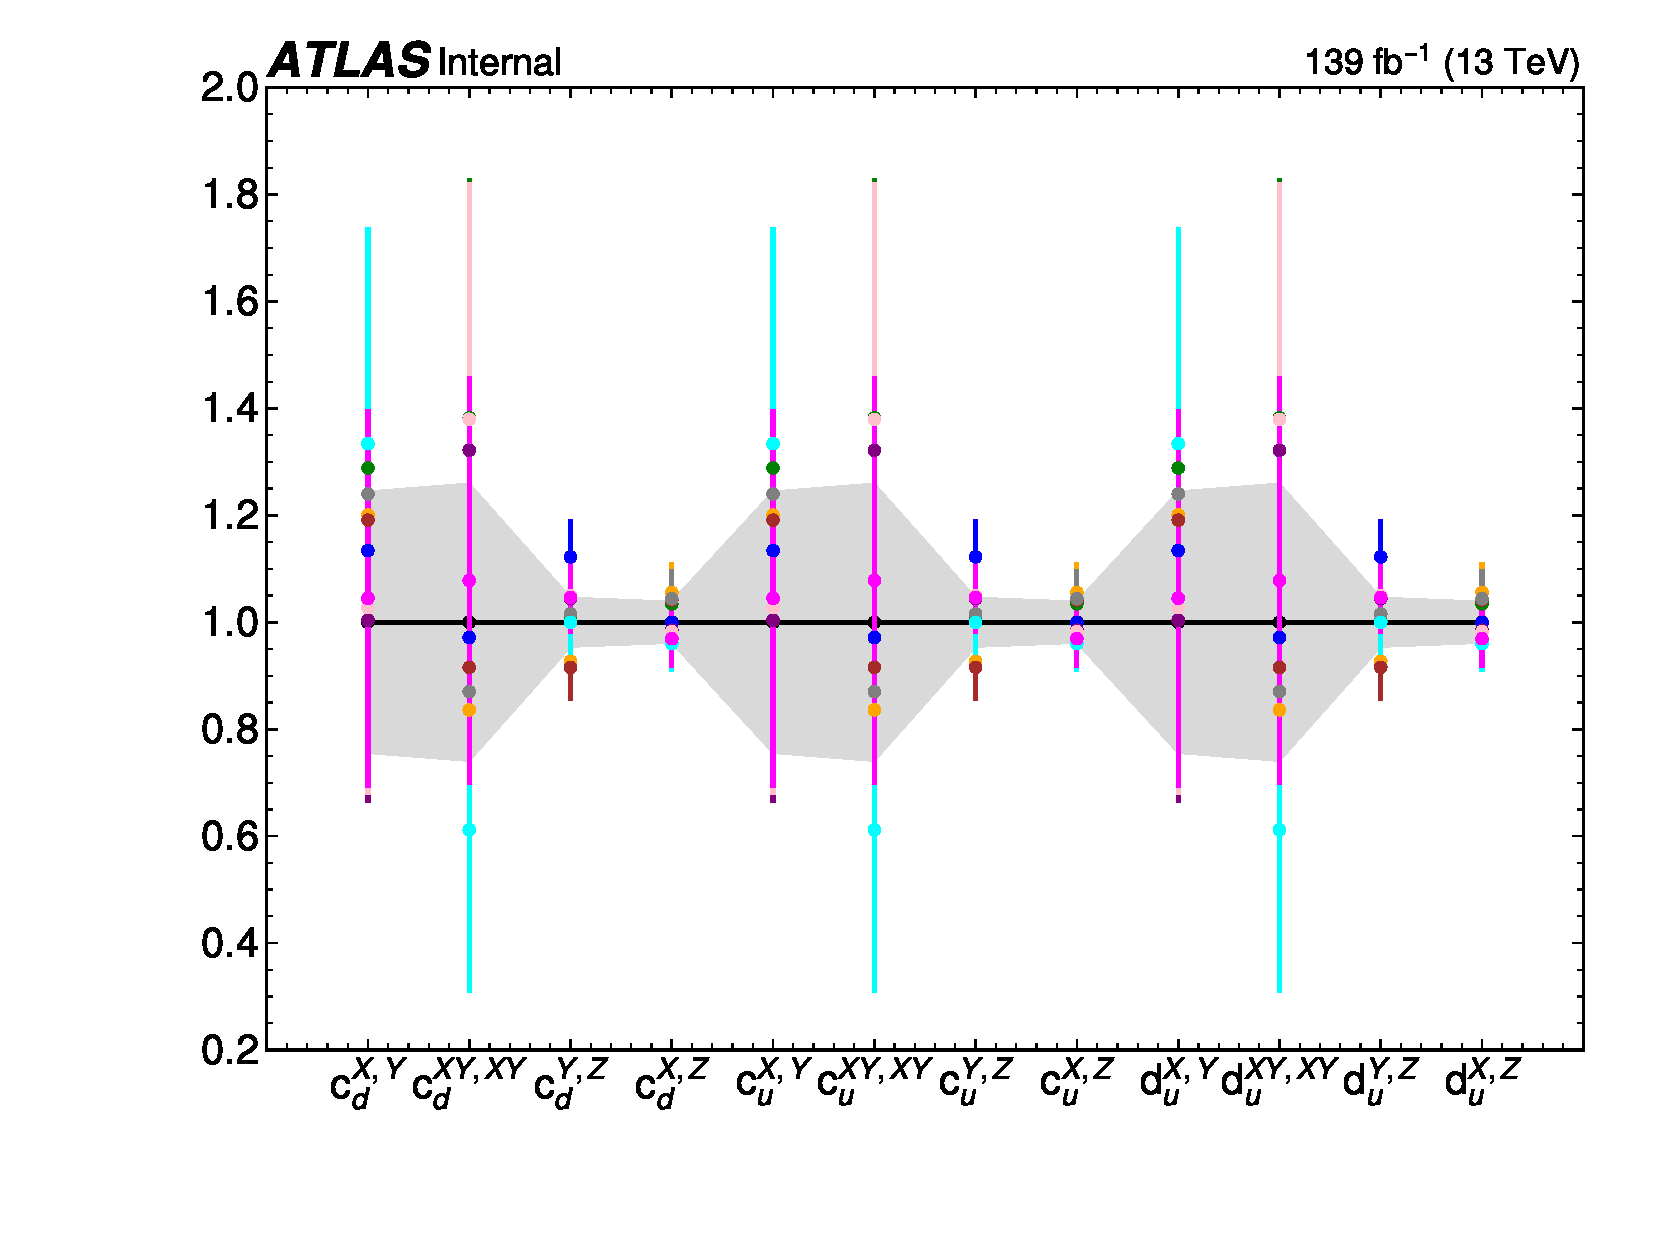
\includegraphics[width=0.45\textwidth]{figs/partially_unblinded_results/scrambled_10K/compare10K_results}
    \caption{The results in each batchs}
    \label{fig:compare_10_batches}
\end{figure}




\subsection{Investigate different probing periods}
\label{lab:scrambleddatasets_periods}

We checked scrambled datasets in various probing periods. As the results shown in
 Figure~\ref{fig:scrambled_Xperiods}, we didn't see any strange behavior in various periods.
 The 7 hours period showed slitly larger (compared to other periods) deviations from zeros. Therefore, we checked 6.87 and 7.13
 hours period to check if it is a coinsidence. The results of 6.87, 7, 7.13 hours periods show that 
 the slitly larger deviations is just a coinsidence (not related to a specific period).
\begin{figure}
    \centering
    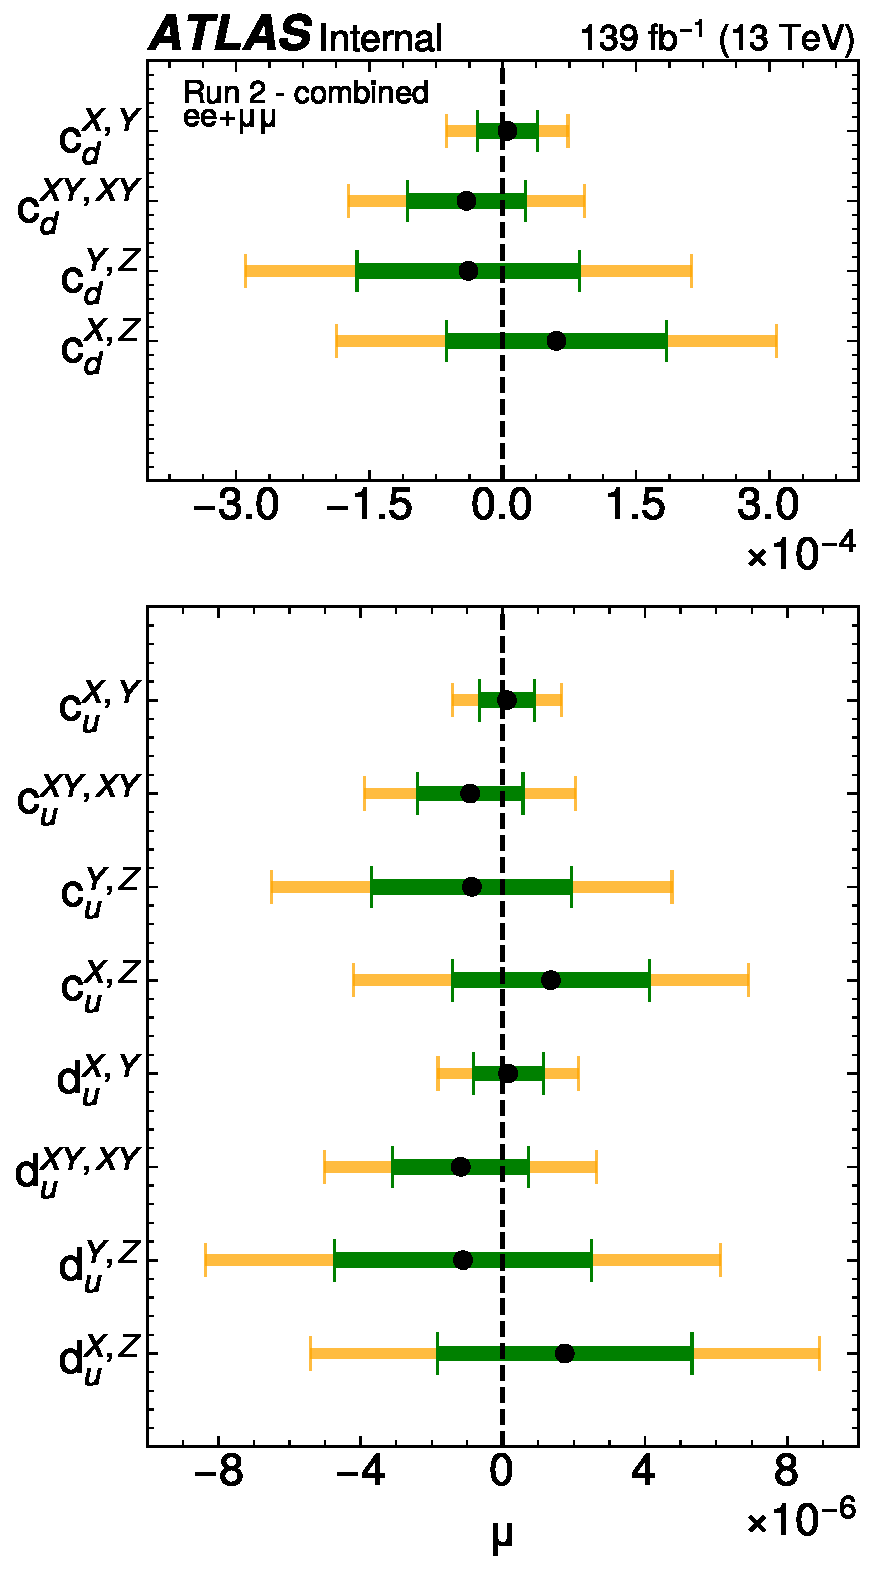
\includegraphics[ width=0.3\textwidth]{figs/partially_unblinded_results/periods/SigFit_summary_AllSamples_Combined_ll_1hour}
    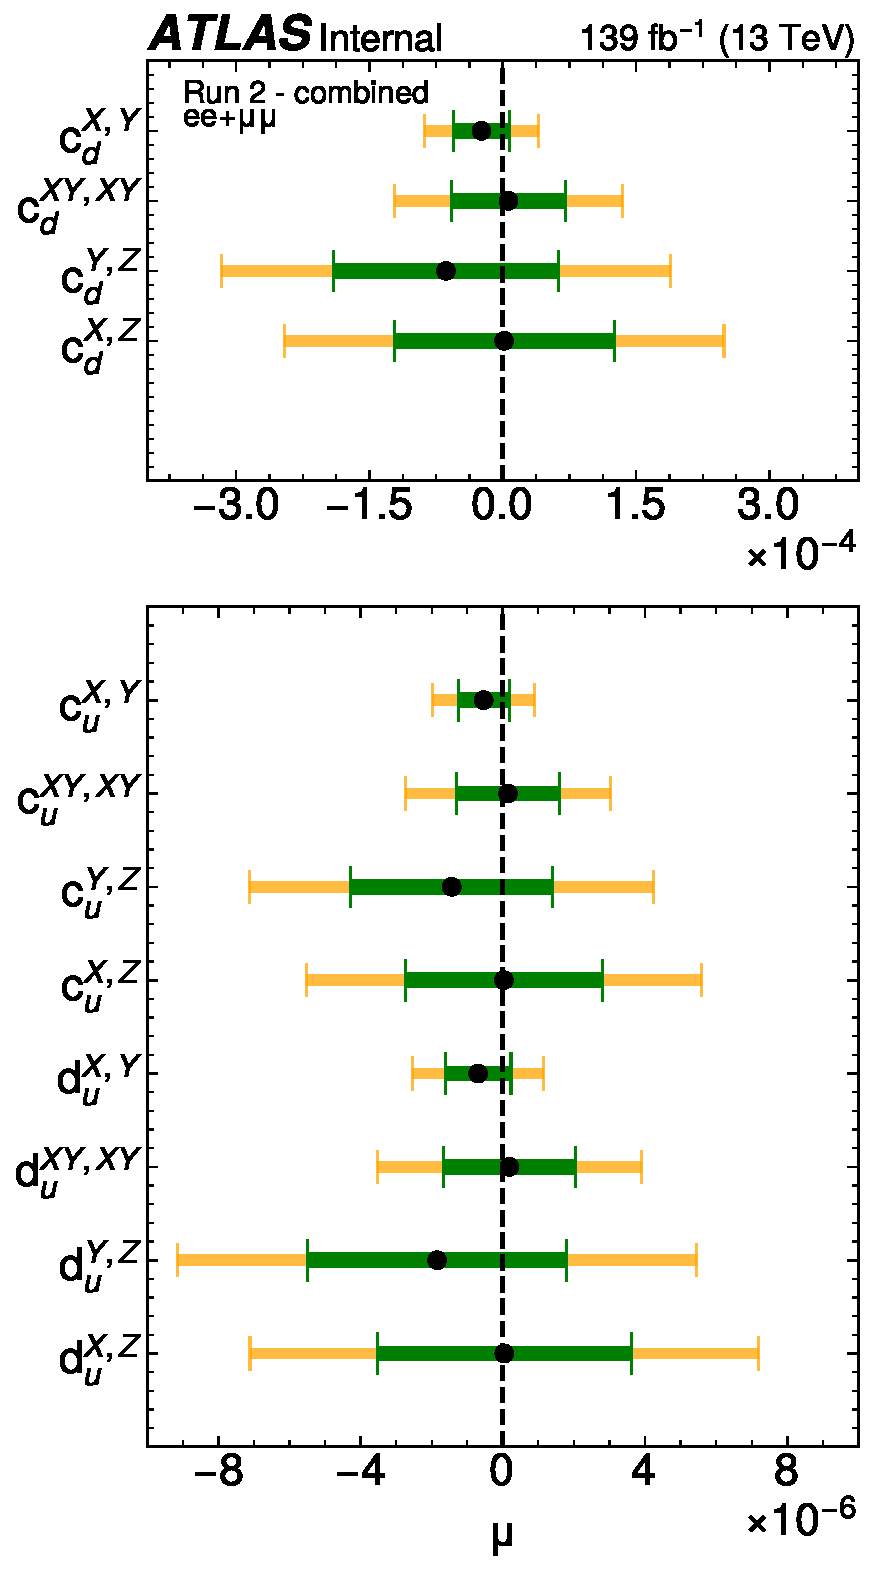
\includegraphics[ width=0.3\textwidth]{figs/partially_unblinded_results/periods/SigFit_summary_AllSamples_Combined_ll_24hour}
    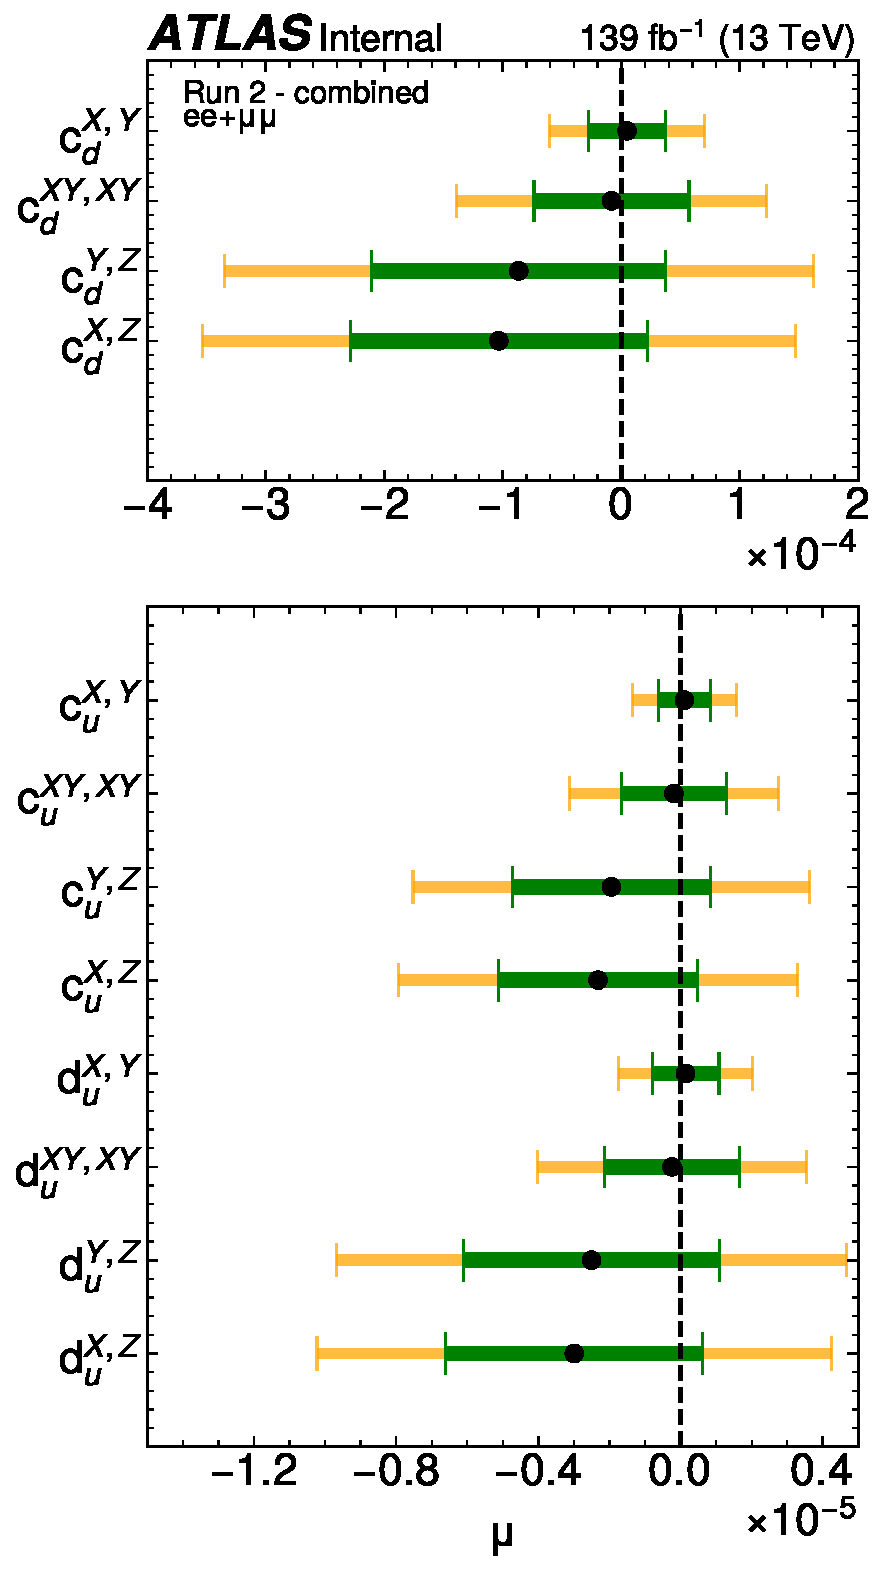
\includegraphics[ width=0.3\textwidth]{figs/partially_unblinded_results/periods/SigFit_summary_AllSamples_Combined_ll_sidereal_10K}\\
    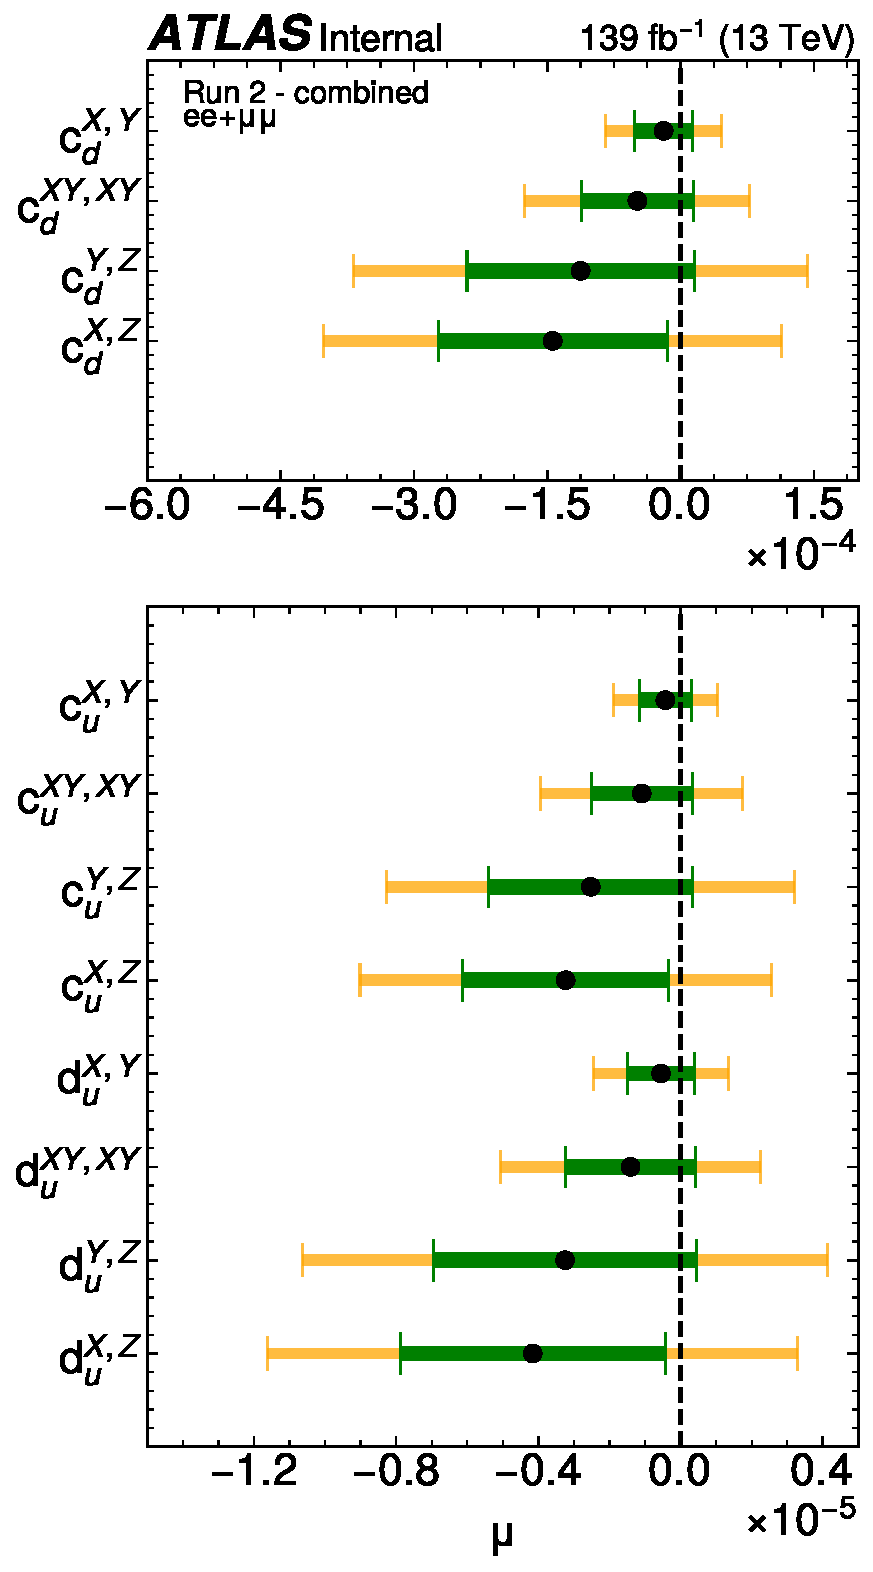
\includegraphics[ width=0.3\textwidth]{figs/partially_unblinded_results/periods/SigFit_summary_AllSamples_Combined_ll_6_87hour}
    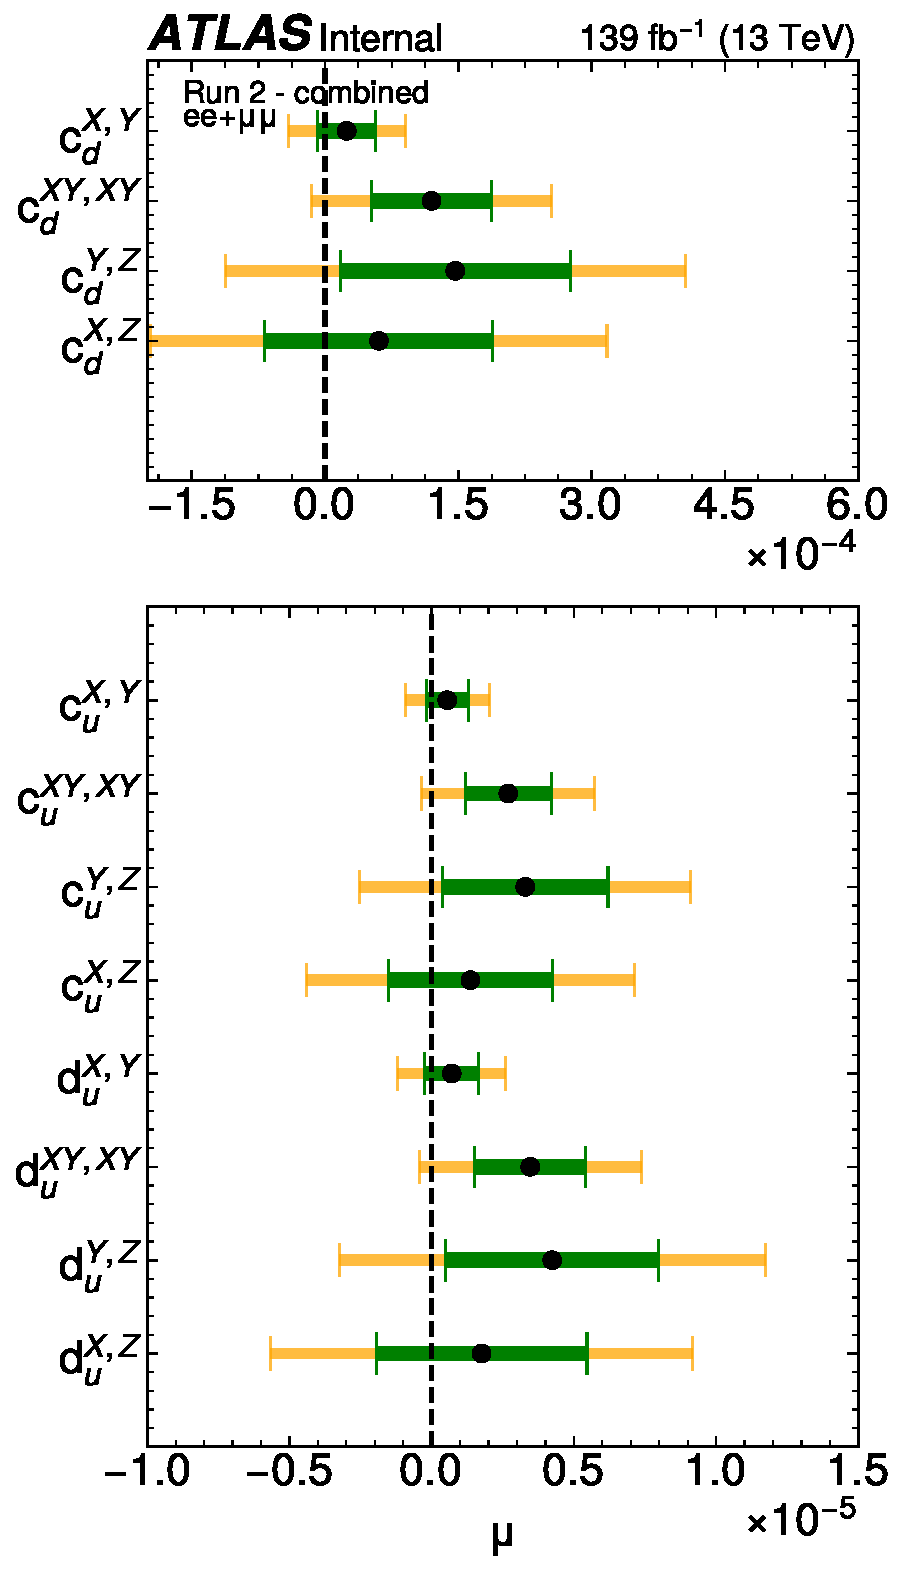
\includegraphics[ width=0.3\textwidth]{figs/partially_unblinded_results/periods/SigFit_summary_AllSamples_Combined_ll_7hour}
    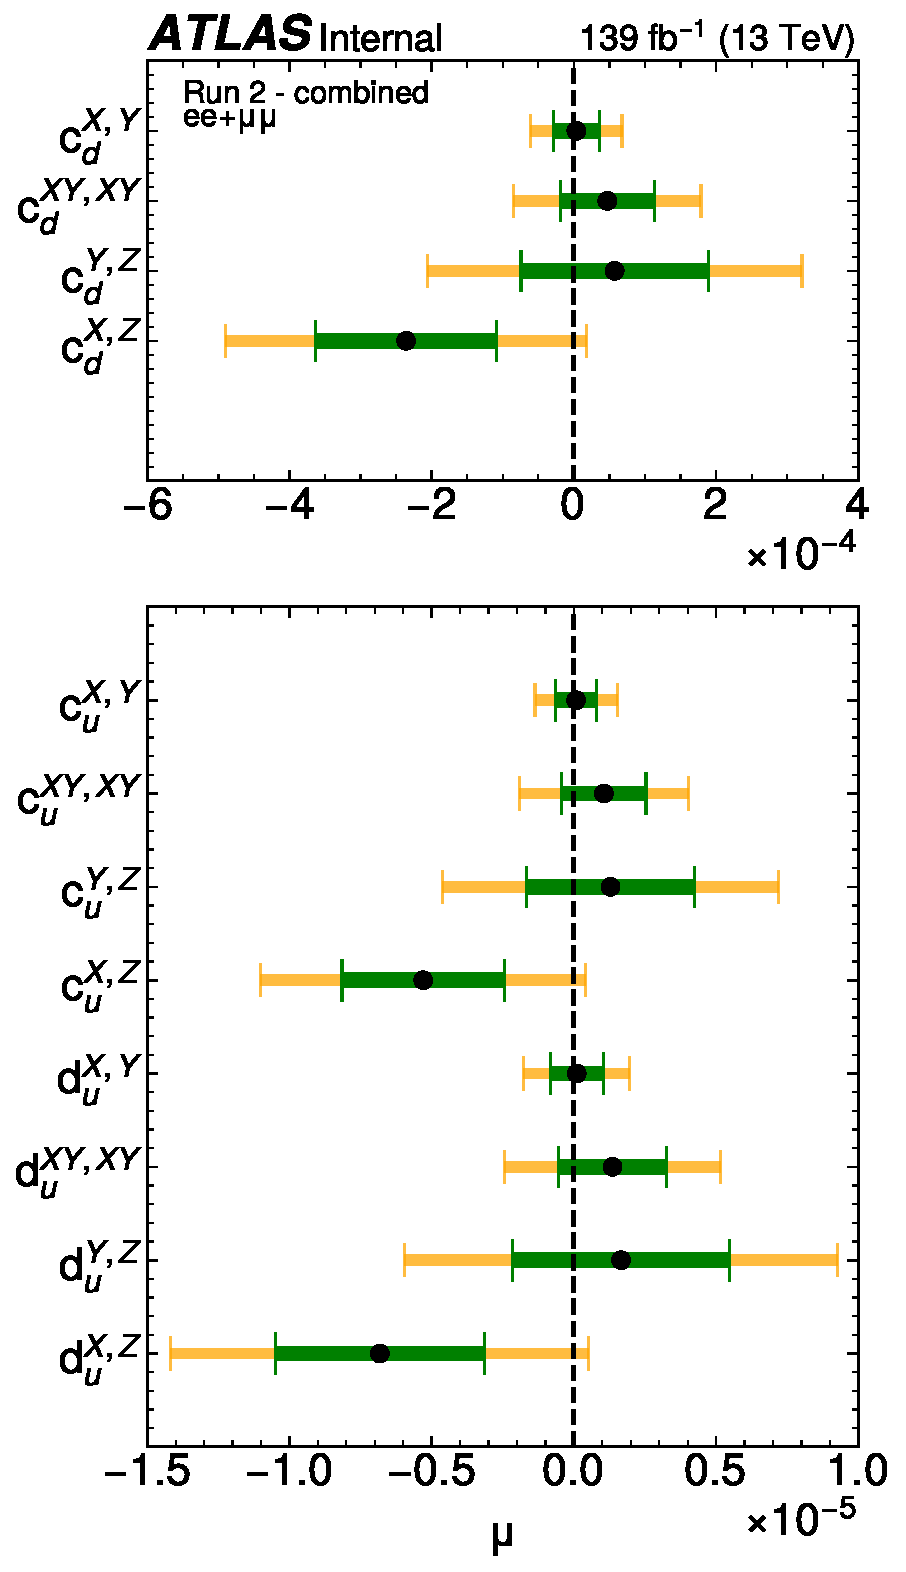
\includegraphics[ width=0.3\textwidth]{figs/partially_unblinded_results/periods/SigFit_summary_AllSamples_Combined_ll_7_13hour}

    \caption{Results of scrambled datasets in 1 hour (top left), 24 hours (top middle), 
    sidereal (top right), 6.87 hours (bottom left), 7 hours (bottom middle), and 
     7.13 hours (bottom right) periods. Results are the average of 1000 fit 
     results (the sidereal period used 10000 fit results).}
    \label{fig:scrambled_Xperiods}
\end{figure}



Figure~\ref{fig:scrambled_Xperiods_Spreads_Stats} shows Spreads VS average stats
 in 1, 6.87, 7, 7.13, 24 hours and sidereal periods. Detail of Spreads and Average Stats are described 
 in Section~\ref{sec:Spread_VS_Stats}.

\begin{figure}[hp]
    \centering
    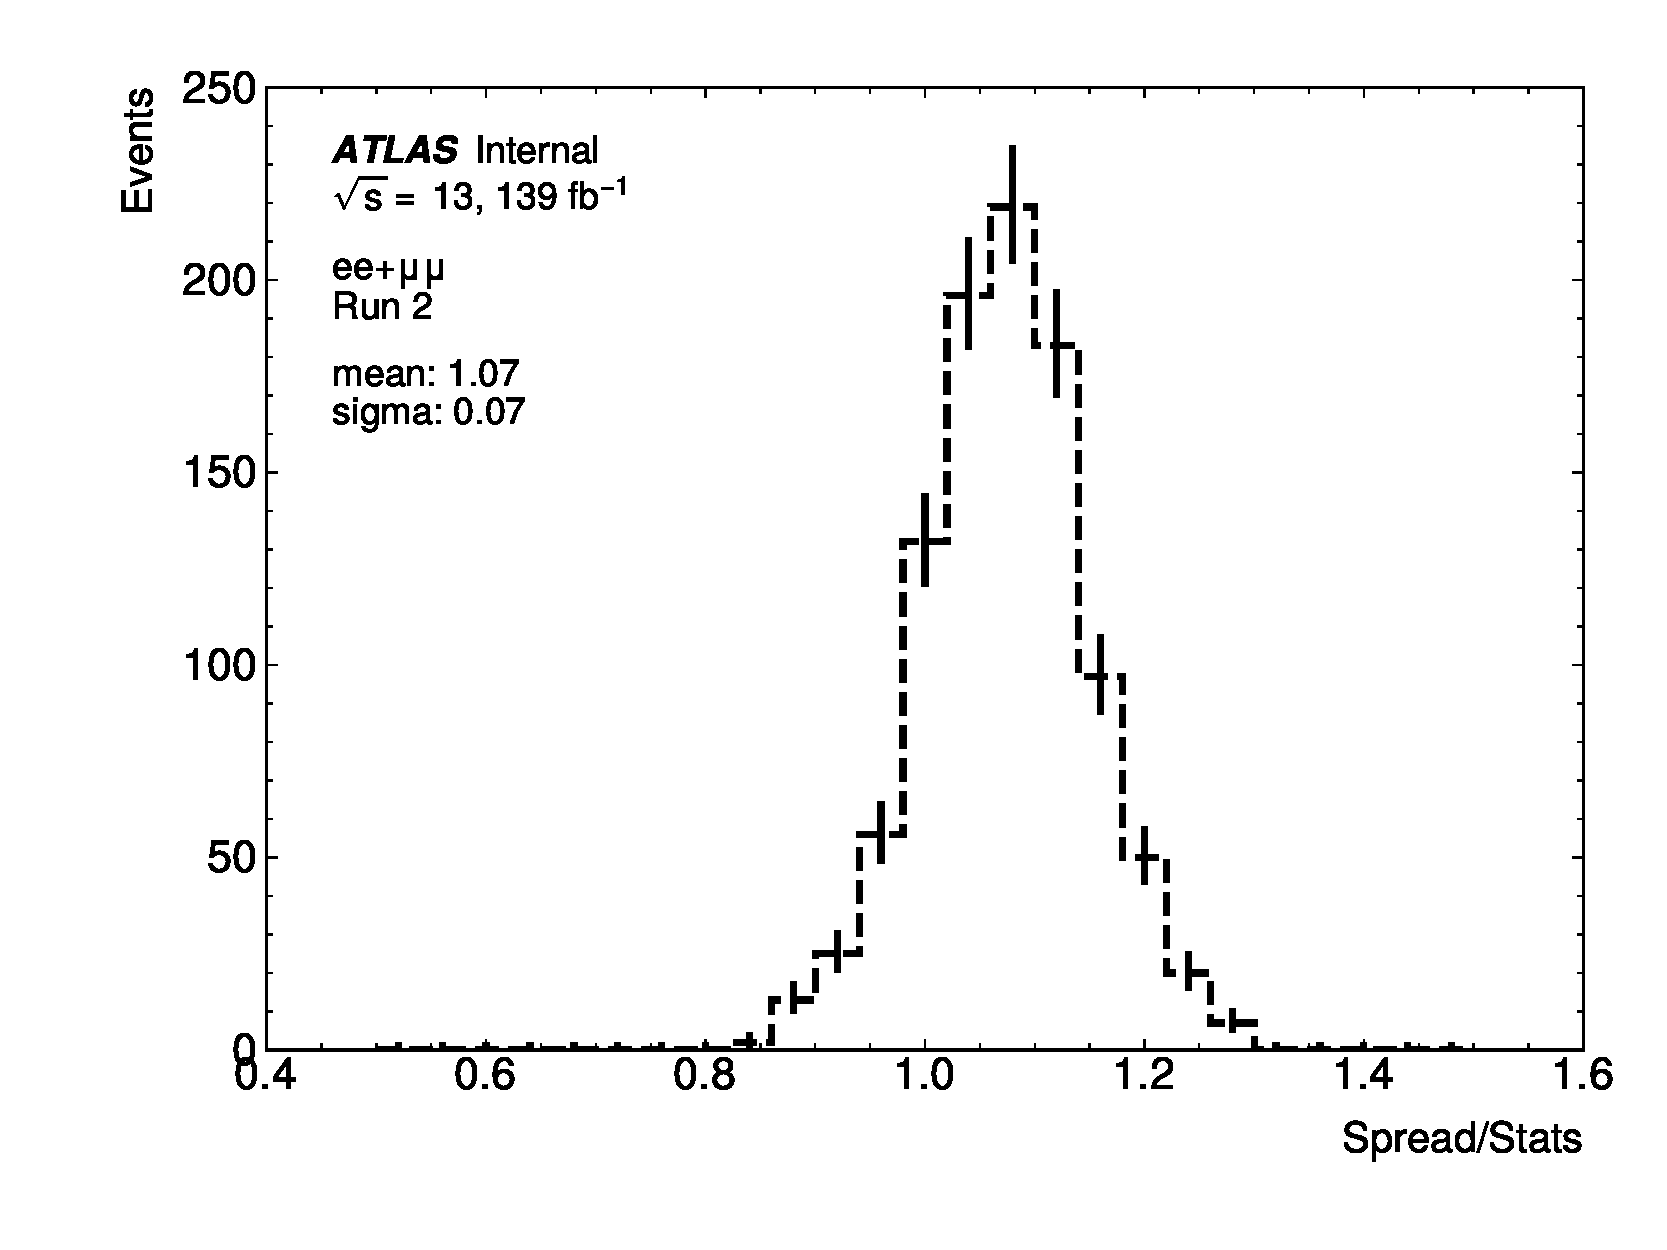
\includegraphics[width=0.3\textwidth]{figs/partially_unblinded_results/periods/spread_stats_scrambled_full_Ratio_1hour}
    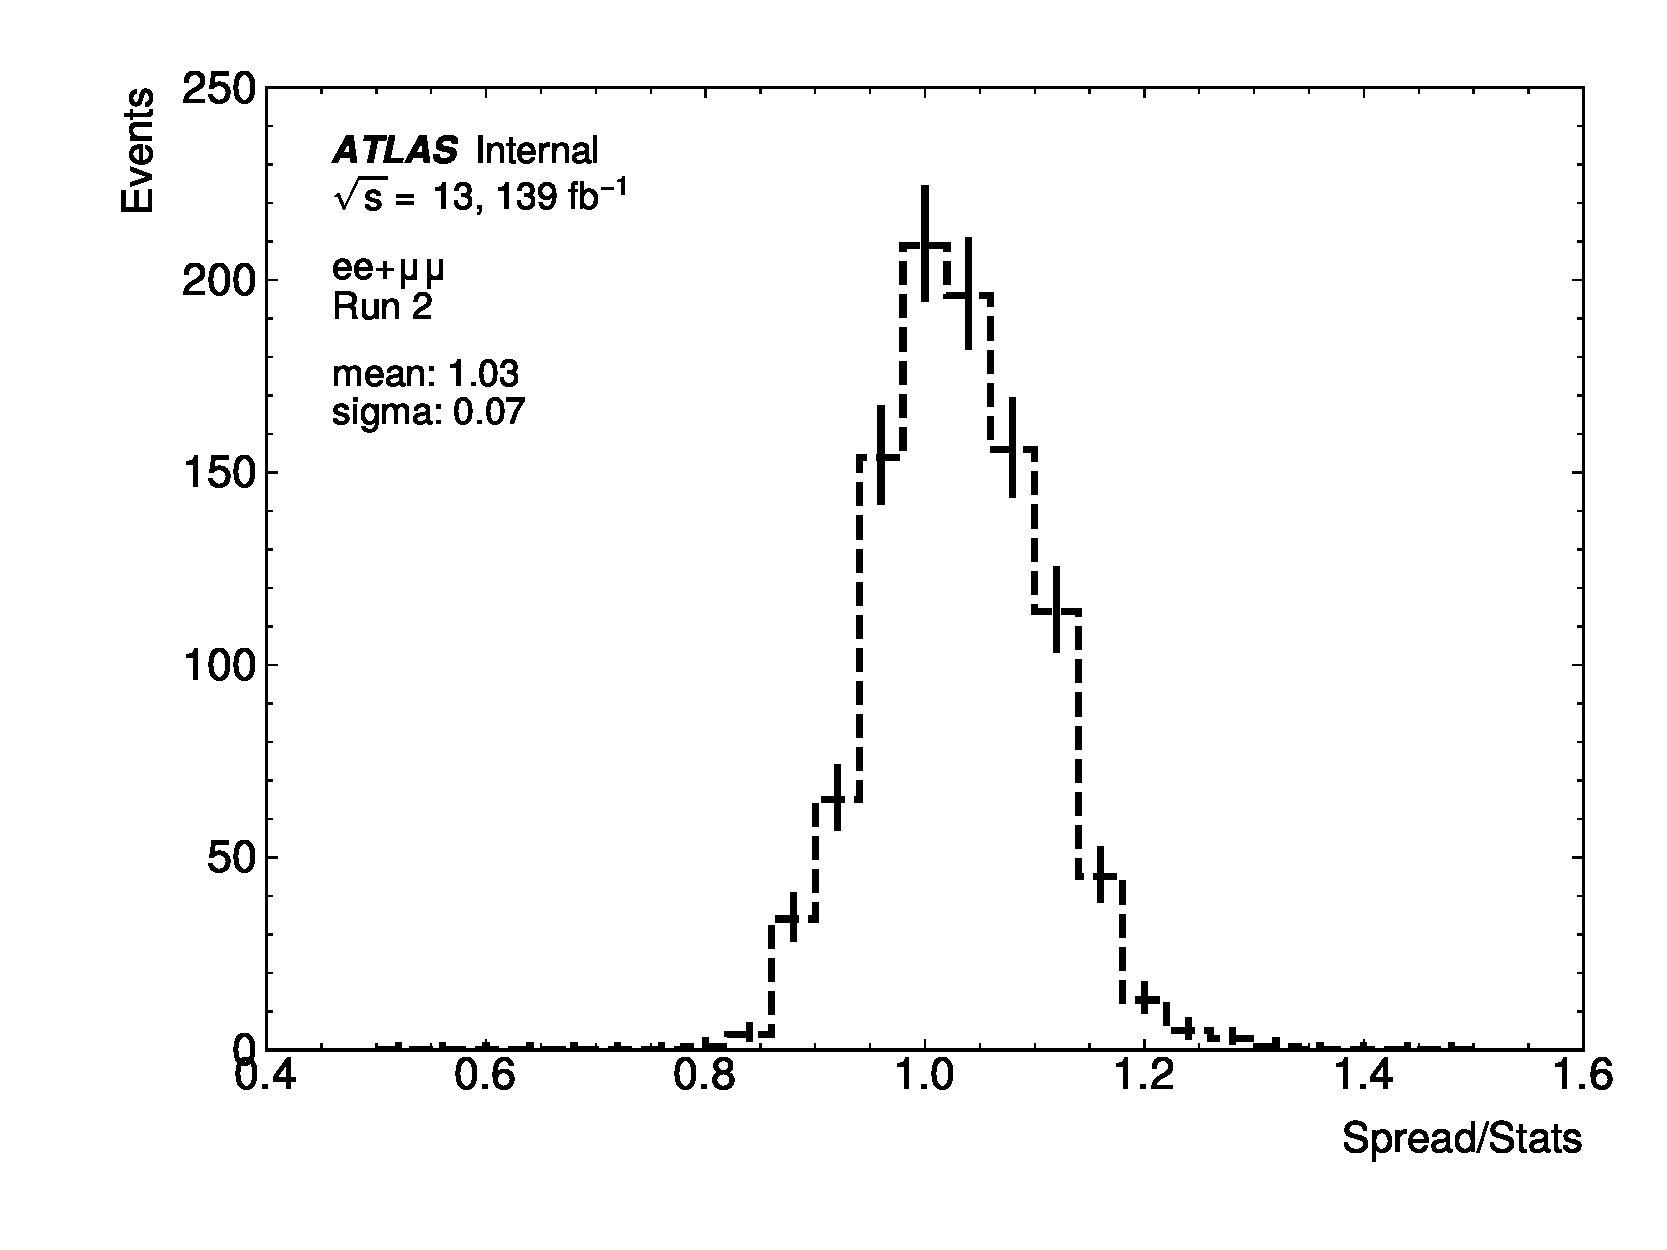
\includegraphics[width=0.3\textwidth]{figs/partially_unblinded_results/periods/spread_stats_scrambled_full_Ratio_6_87hour}
    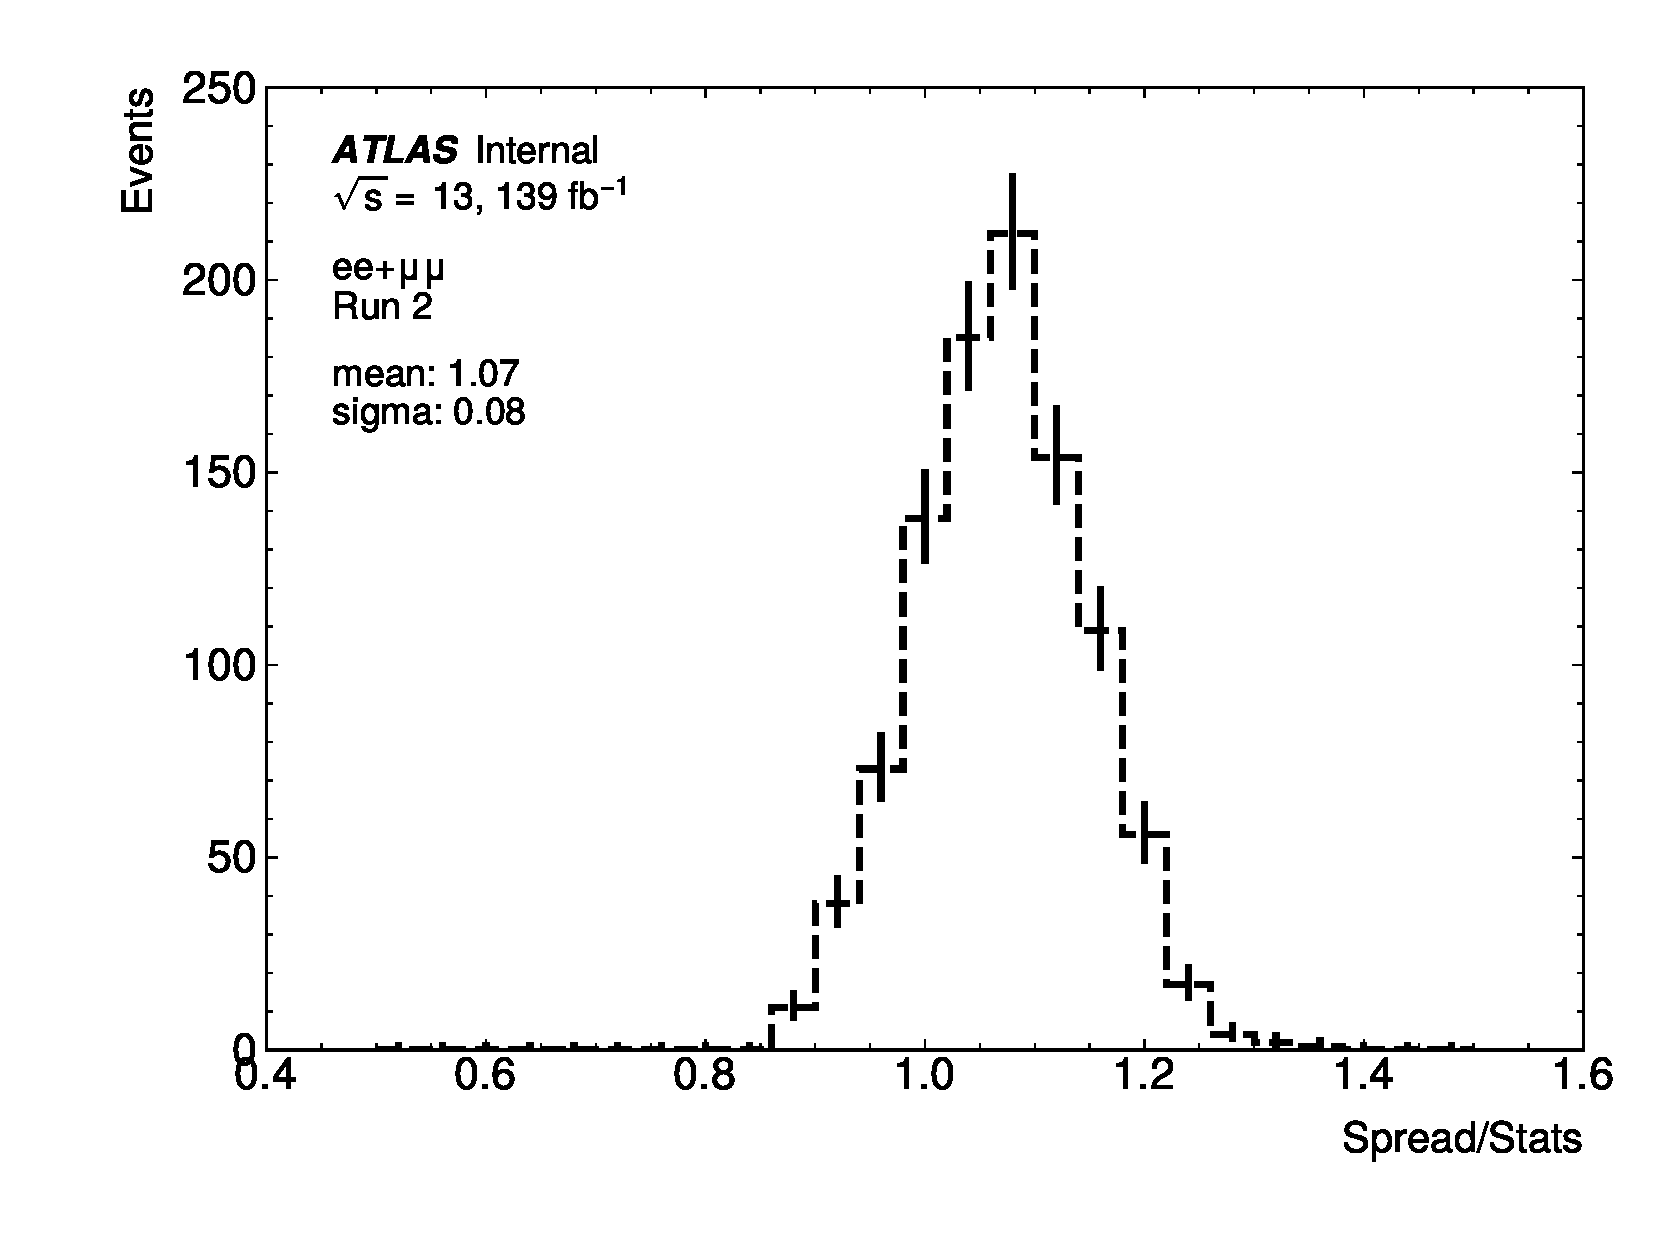
\includegraphics[width=0.3\textwidth]{figs/partially_unblinded_results/periods/spread_stats_scrambled_full_Ratio_7hour}\\
    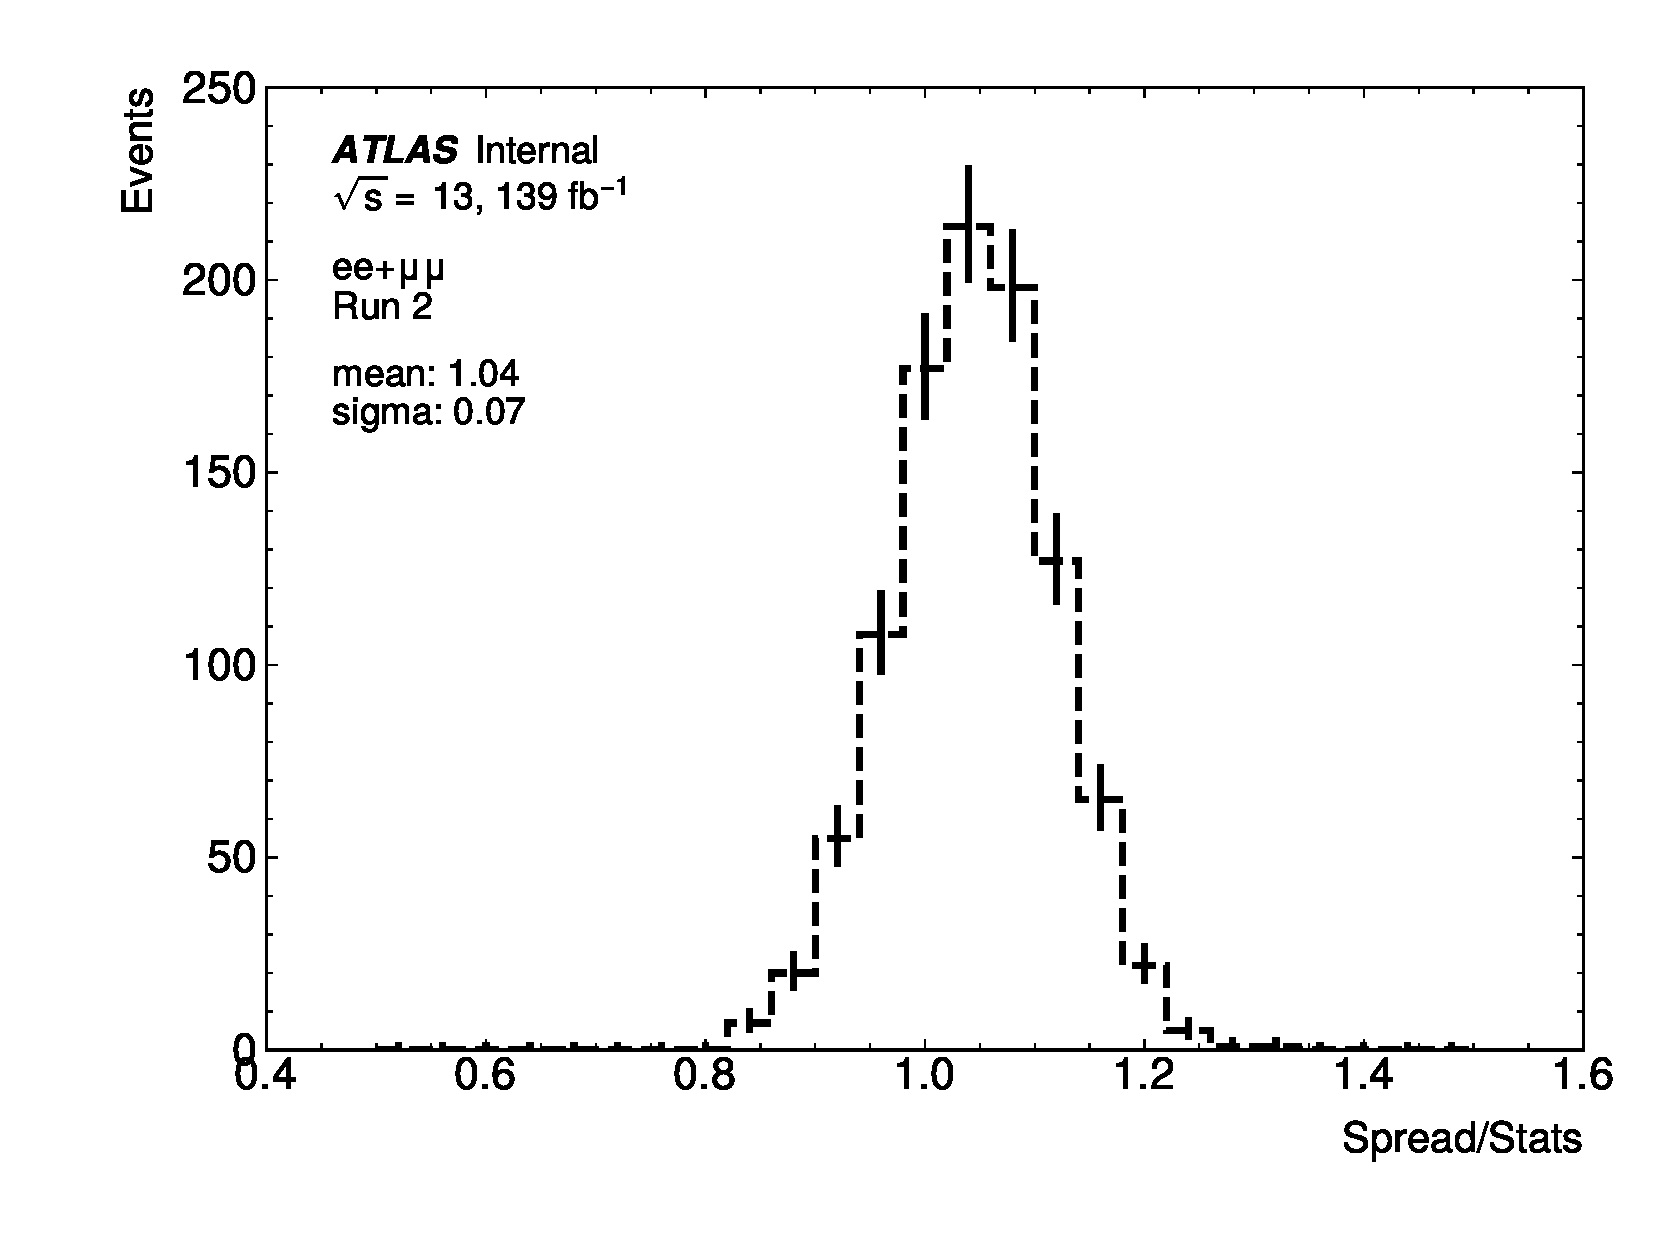
\includegraphics[width=0.3\textwidth]{figs/partially_unblinded_results/periods/spread_stats_scrambled_full_Ratio_7_13hour}
    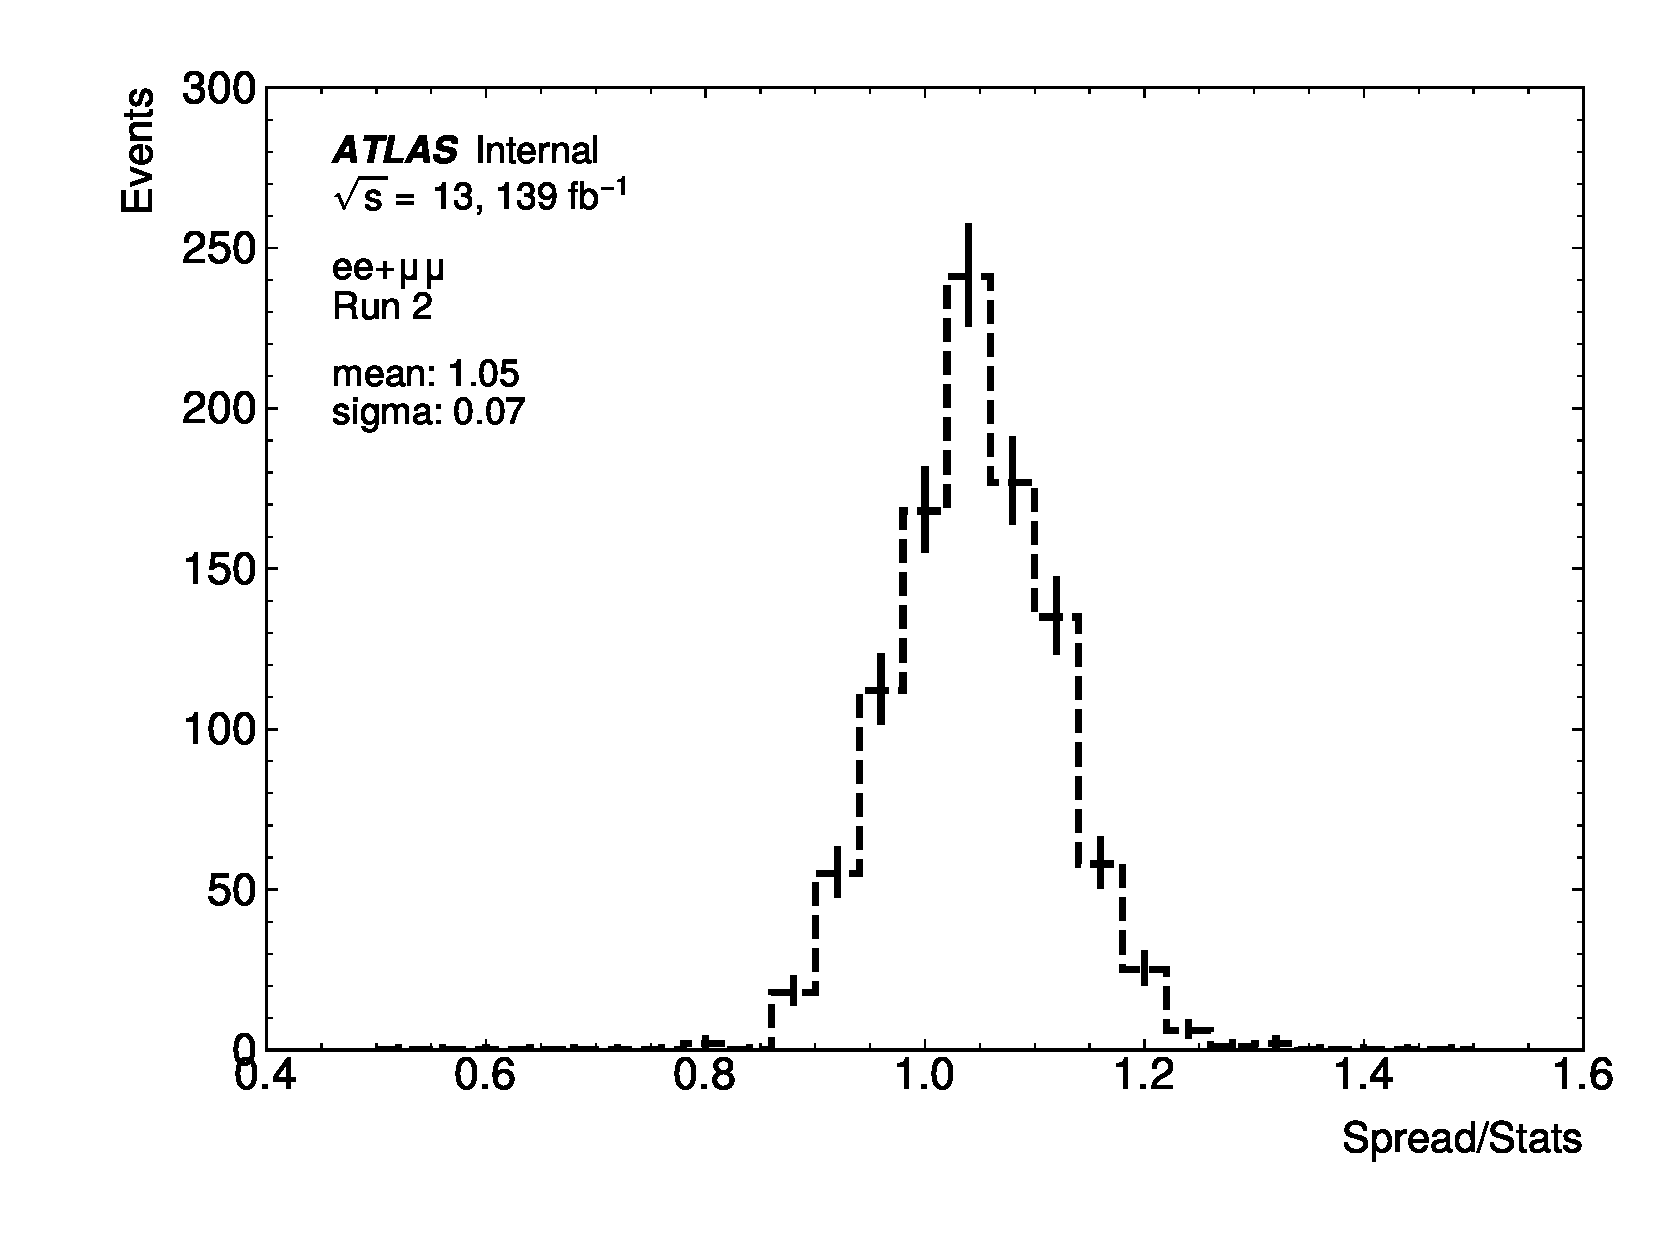
\includegraphics[width=0.3\textwidth]{figs/partially_unblinded_results/periods/spread_stats_scrambled_full_Ratio_24hour}
    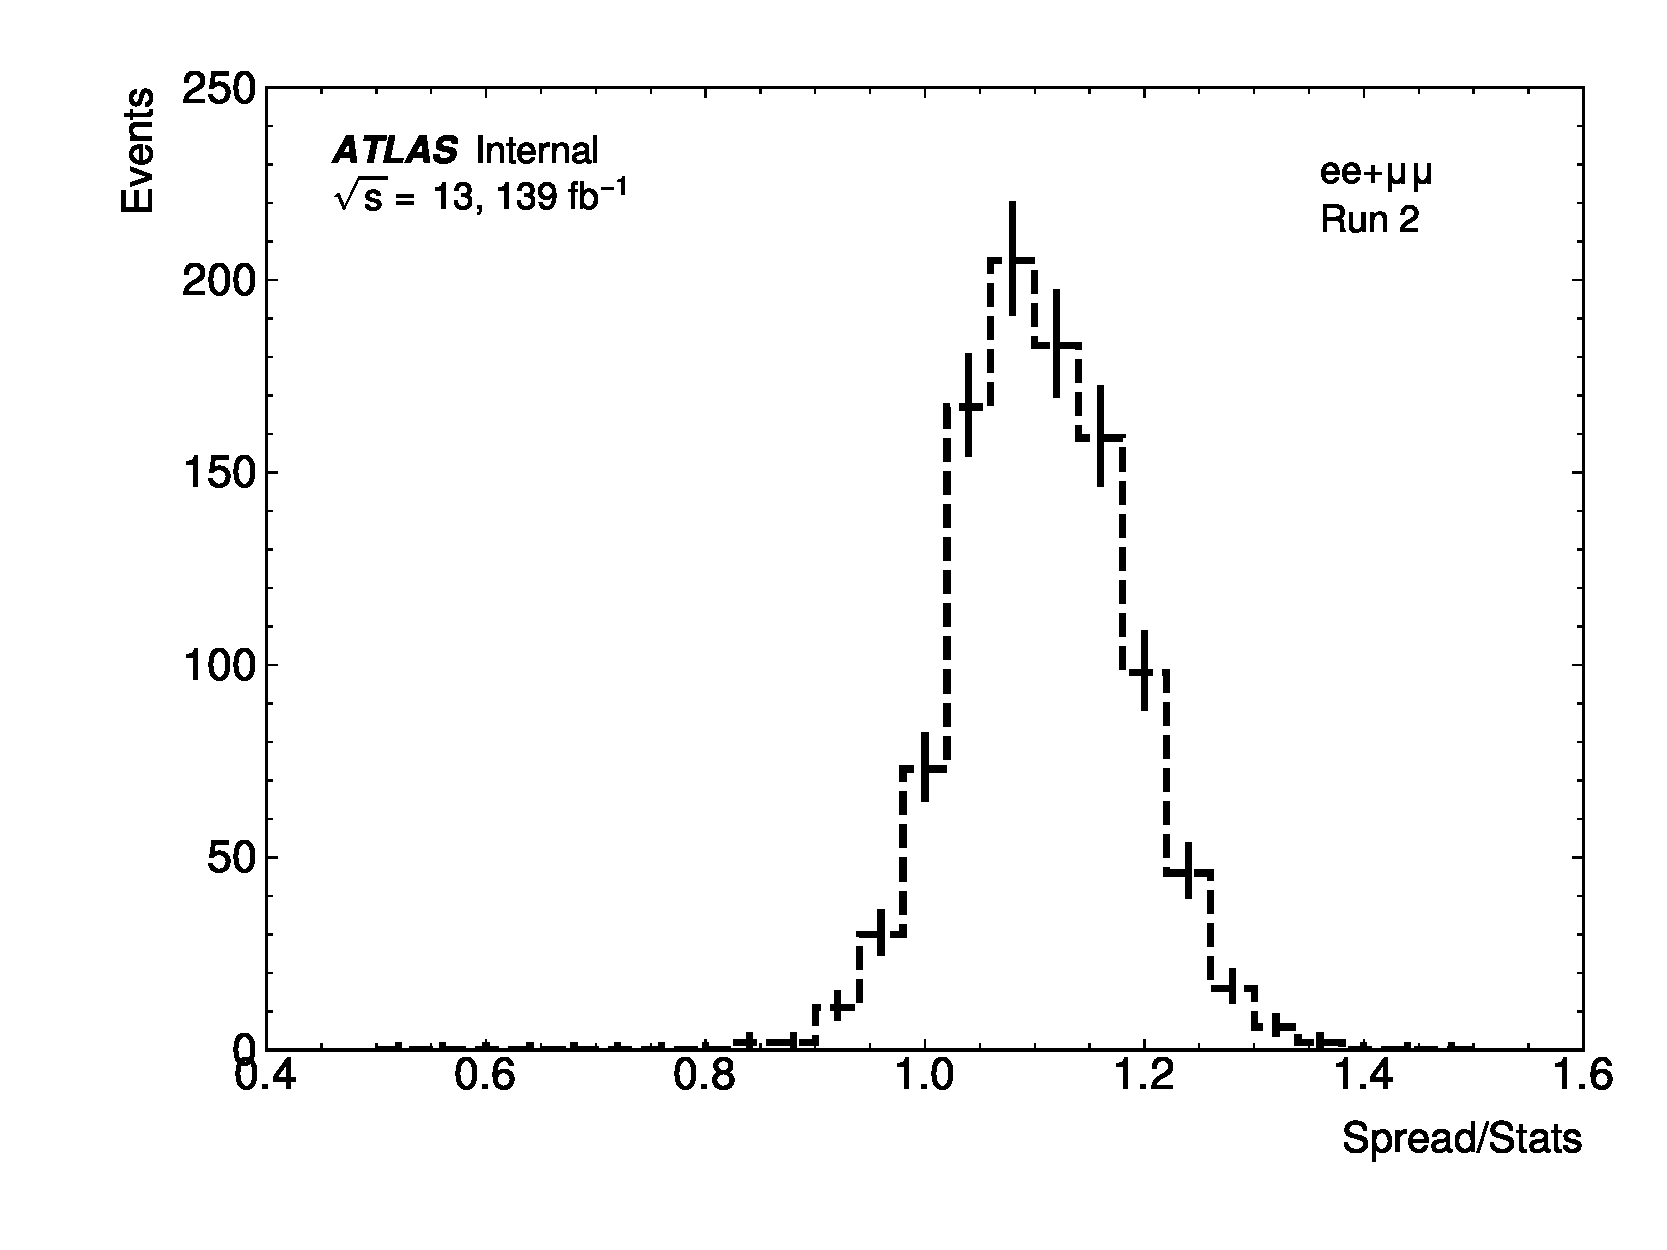
\includegraphics[width=0.3\textwidth]{figs/partially_unblinded_results/periods/spread_stats_scrambled_full_Ratio_sidereal}
    \caption{Left to right: 1, 6.87 and 7 hours perios (top plots); 7.13, 24 hours and sidereal perios (bottom plots).
    Spreads VS average stats. Plots show average results of 1000 scrambled datasets. 
    An average statistic is the average statistical uncertainty in each scrambled dataset, 
    and the spread of a dataset is an average of absolute residual.
    Spread is about 10-20\% larger in most of the scrambled datasets. This indicates there
     is a small systematic effect or the way we are calculating the ZC error in the double 
     ratio. This could be the reason why the average values shifted from zero}
    \label{fig:scrambled_Xperiods_Spreads_Stats}
    \end{figure} %% Ablet


\clearpage
\section{Time-dependent systematic uncertainties} %% [Ablet/Uta]
%\label{lab:Systematic}
%\subsection{Overview of systematic}
\label{lab:Systematic_overvies}

Sources of systematic effects can be considered as nominal analysis in ATLAS, but following items are canceled out by taking the double ratio. 

\begin{itemize}
\item[a] Theory related items, i.e. cross section of all SM processes, QCD scale uncertainty, any kinematic mismodling including higher order calculation in the Matrix element or parton shawer, variation of parton distribution functions. 
\item[b] Most of experimental items, i.e., object reconstruction and identification efficiencies, total luminosity, normalization effects.
\item[c] year by year normnalization effect, i.e., LUCID luminosity measurement variation.
\item[d] mis-measurement on Z counting or LUCID luminosity. 
\item[e] Time dependent effects, i.e.  $\left< \mu \right>$ effect.

\end{itemize}

Only time dependent effects remained as systematic uncertainty, therefore items ``a'' and ``b'' are not the source of systematic on the LIV search.

Concerning to item ``c'', there are variation in the LUCID luminosity measurement, which effect are corrected by van-deer-mir scan. If we sum up all years (2015 to 2018) into one double ratio, this would introduce additional systematic effect, but as we discussed in Section~\ref{lab:DataScrambling}, we build the double ratio each year separately and combine in the final fit. Therefore, this effect is not necessary to take into account.

Nevertheless, item ``d'', mis-measurement on the input of the double ratio could introduce the systematic effect. In order to exclude mis-measurement, LBs have large deviation, i.e. integrated luminosity would be 0 in one of input (either LUCID, electron channel or muon channel of Z counting luminosity) are excluded from the input LB as additional data quality requirement. 


The item ``e'' is the systematic source we need to take into account. Actully, the Z counting luminosity measurement does takes into account variation of the trigger and the identification  efficiencies for each LB. 
Therefore, even efficiency variation (in item ``c'') is NOT the dominat source of systematic effect for this analysis.  The statistics uncertainty of 
the efficiency correction in each LB is taken into account and propagaed to the error bar of each phase bin of the double ratio. 

There is a correction factor as function of  $\left< \mu \right>$ in the Z counting measurement, which is FMC correction factor. 
The $\left< \mu \right>$ dependence of $F^\text{MC}_{Z\rightarrow \ell^+\ell^-}$ is fitted with a second-order polynomial per decay channel 
and per data-taking period, and the fit results are shown in Figure~\ref{fig:Zcount:MC correction factors}.

The $Z\rightarrow e^+e^-$ correction factor is >10\% below unity for all $\left< \mu \right>$, implying that there are additional efficiency 
effects beyond those captured in the tag-and-probe procedure. The variation between $\left< \mu \right>=20$ and $\left< \mu \right>=50$ is 
around 2\%, suggesting that pileup-dependent effects are mild.

\begin{figure}[!htb]
        \centering
        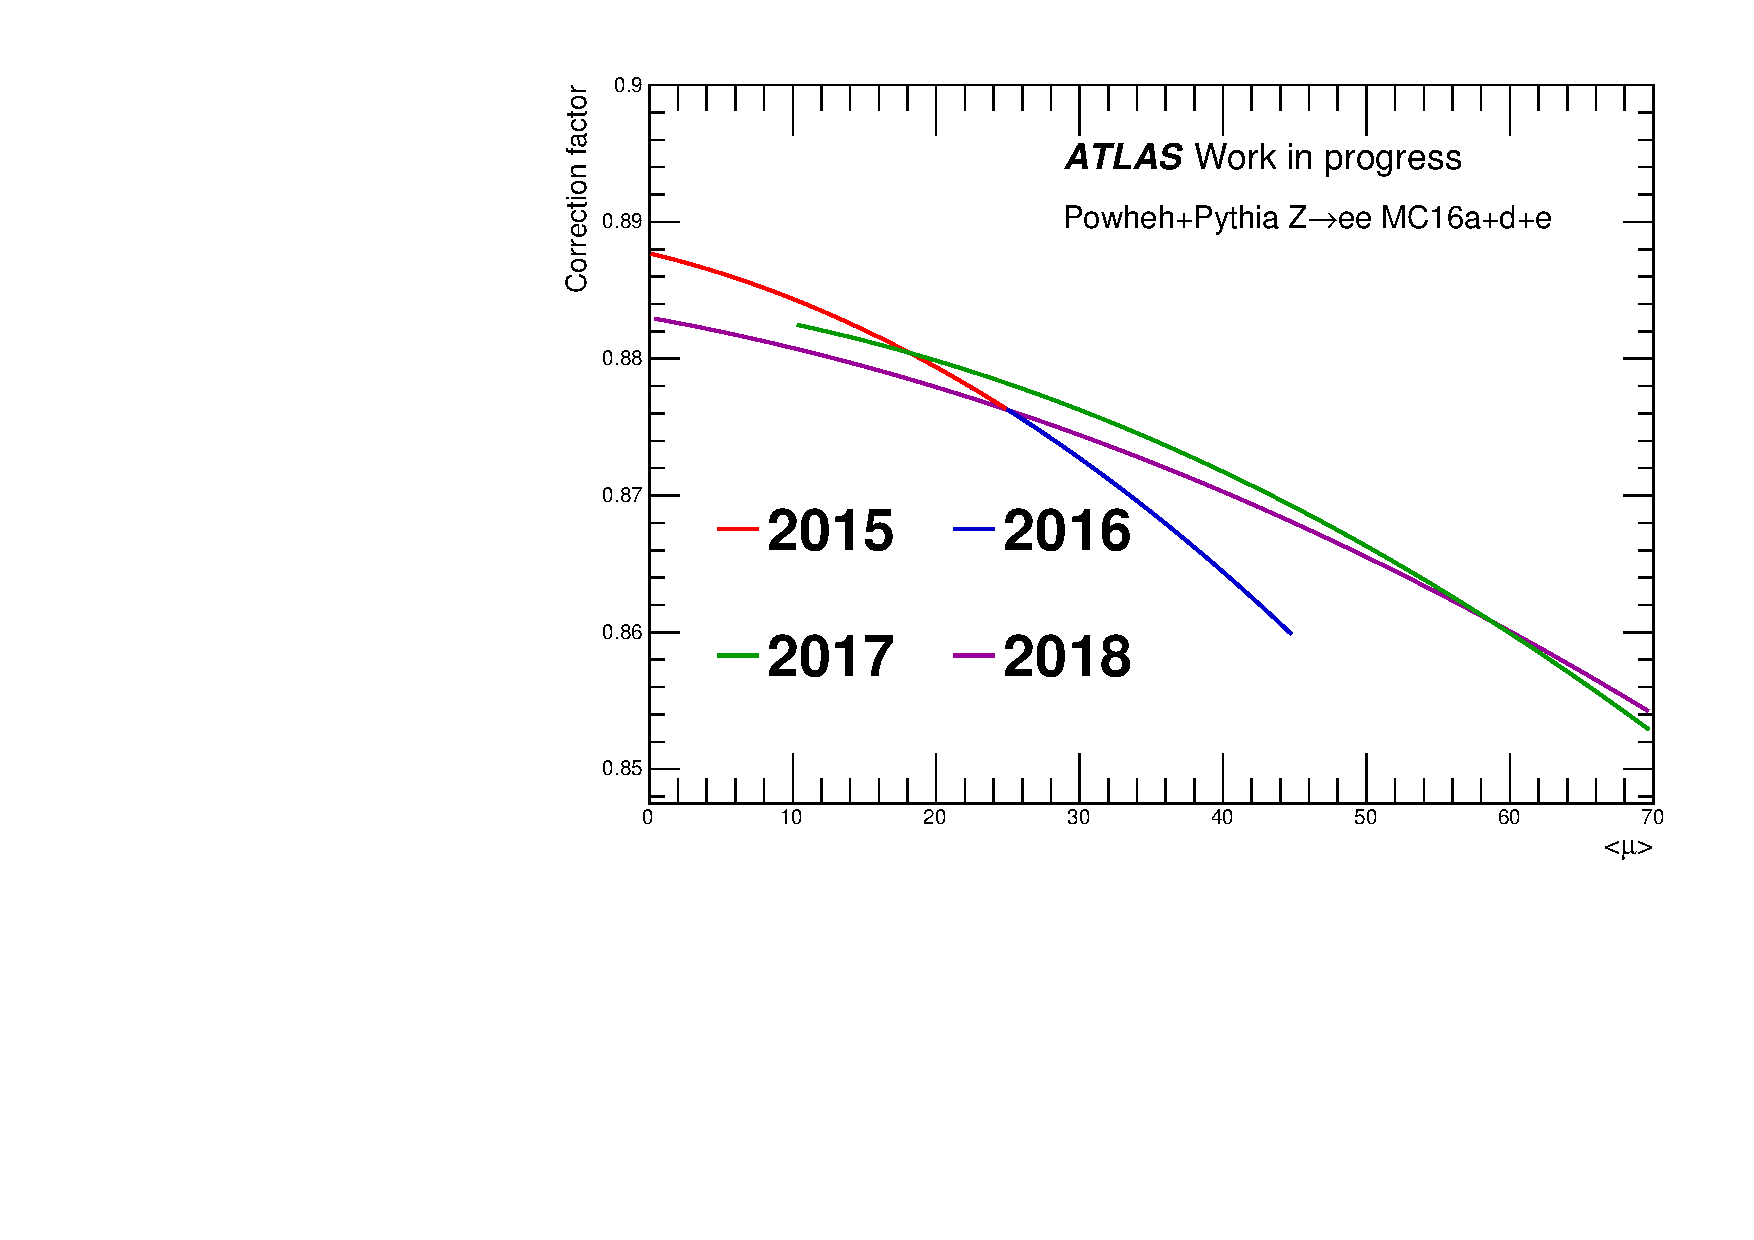
\includegraphics[width=0.6\textwidth]{figs/Zcount/YearlyFMC_ele.pdf}
        \caption{$Z\rightarrow e^+e^-$ correction factors used for each year of data produced using the dedicated Monte Carlo campaigns. The 
          lines show second-order polynomial fits to the correction factor for the corresponding $\left< \mu \right>$ range per year.}
        \label{fig:Zcount:MC correction factors}
\end{figure}

The fits of $F^\text{MC}_{Z\rightarrow \ell^+\ell^-}$, as shown in Figure~\ref{fig:Zcount:MC correction factors}, 
are used in the determination of the Z-counting based luminosity per data-taking period and as a function of the 
pileup parameter $\left< \mu \right>$. The statistical uncertainties of the fits are small and are neglected.

The size of systematic on the FMC corrction is estimated by shifting $\left< \mu \right>$ by $\pm 1$ to apply correction. 
This is done by the TOY study described in Section.~\label{lab:ToyStudy}. Figure~\ref{fig:FMC_variation} shows the effect in the double ratio in a Toy experiment. Result with 1000 Toy experiments are summarized in Figure~\ref{fig:FMC_variation_summary}. We observed this effect is small with respect to statistical uncertainty.

%%%%%%%%%%%%%%%%%%%%%%%%%%%%%%%%%%%%%%%%%%%%%%%%%%%%%%
%%%%%%%%%%%%%%%%%%%%%%%%%%%%%%%%%%%%%%%%%%%%%%%%%%%%%%
%%%%%%%%%%%%%%%%%%%%%%%%%%%%%%%%%%%%%%%%%%%%%%%%%%%%%%
%% \subsection{Shift $<\mu>$ by 1}

\begin{figure}[bt]
\centering
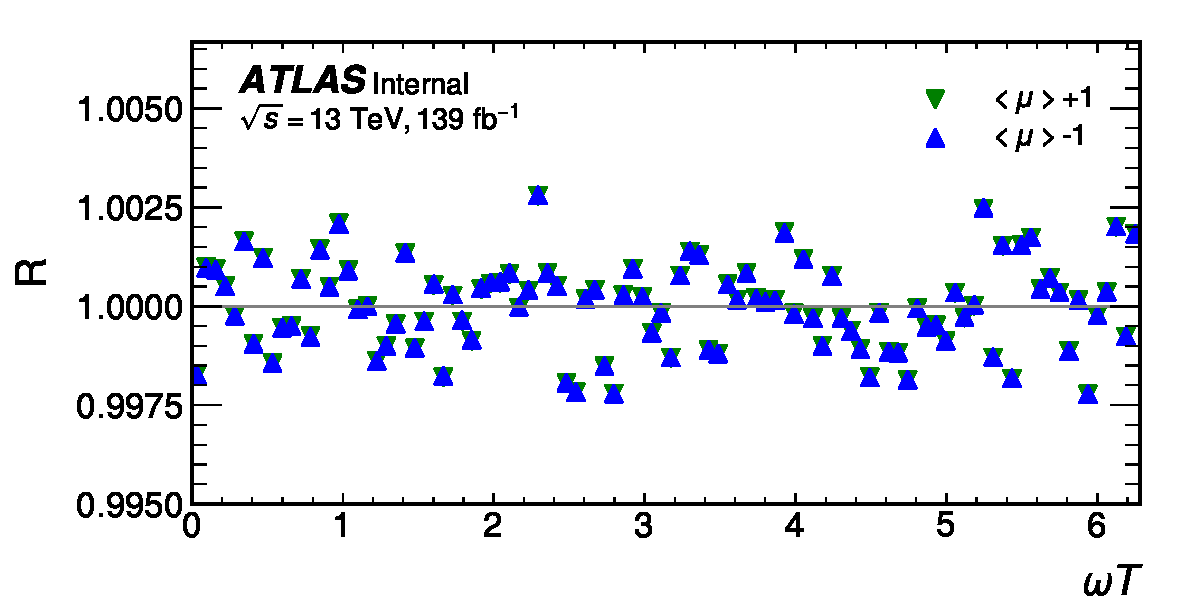
\includegraphics[width=0.95\textwidth]{figs/FMC_sys/compare_input_toy_datasets_mu_shifts} \\
\caption{ Comparison of the toy dataset with average pileup $<\mu>$ increased and decreased by 1. The toy dataset corresponds to four years of Run 2 luminosity is used. The X-axis is the sidereal phase, $\omega T$.
}
\label{fig:FMC_variation}
\end{figure}


\begin{figure}[bt]
\centering
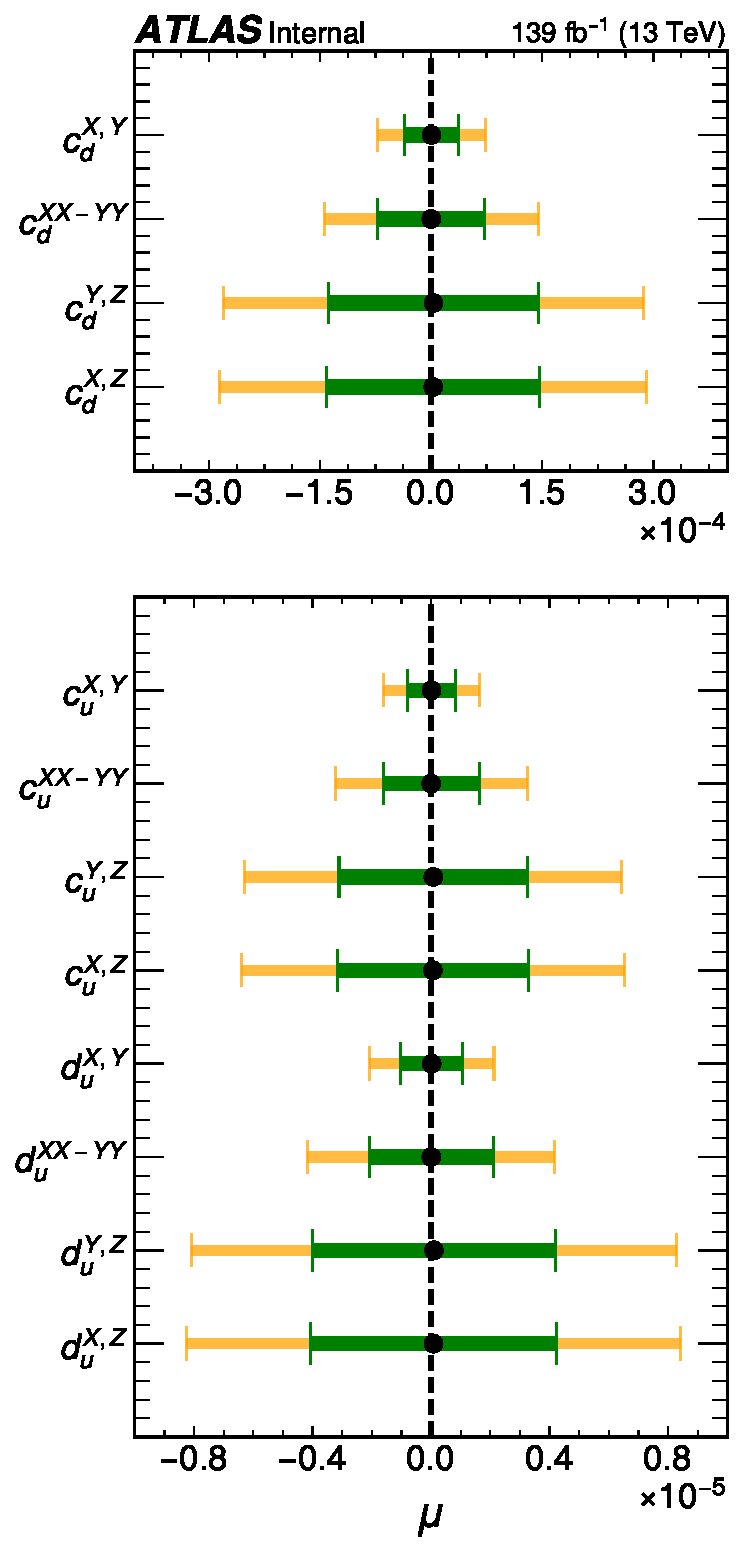
\includegraphics[width=0.4\textwidth]{figs/FMC_sys/SigFit_summary_AllSamples_muShift_p1} 
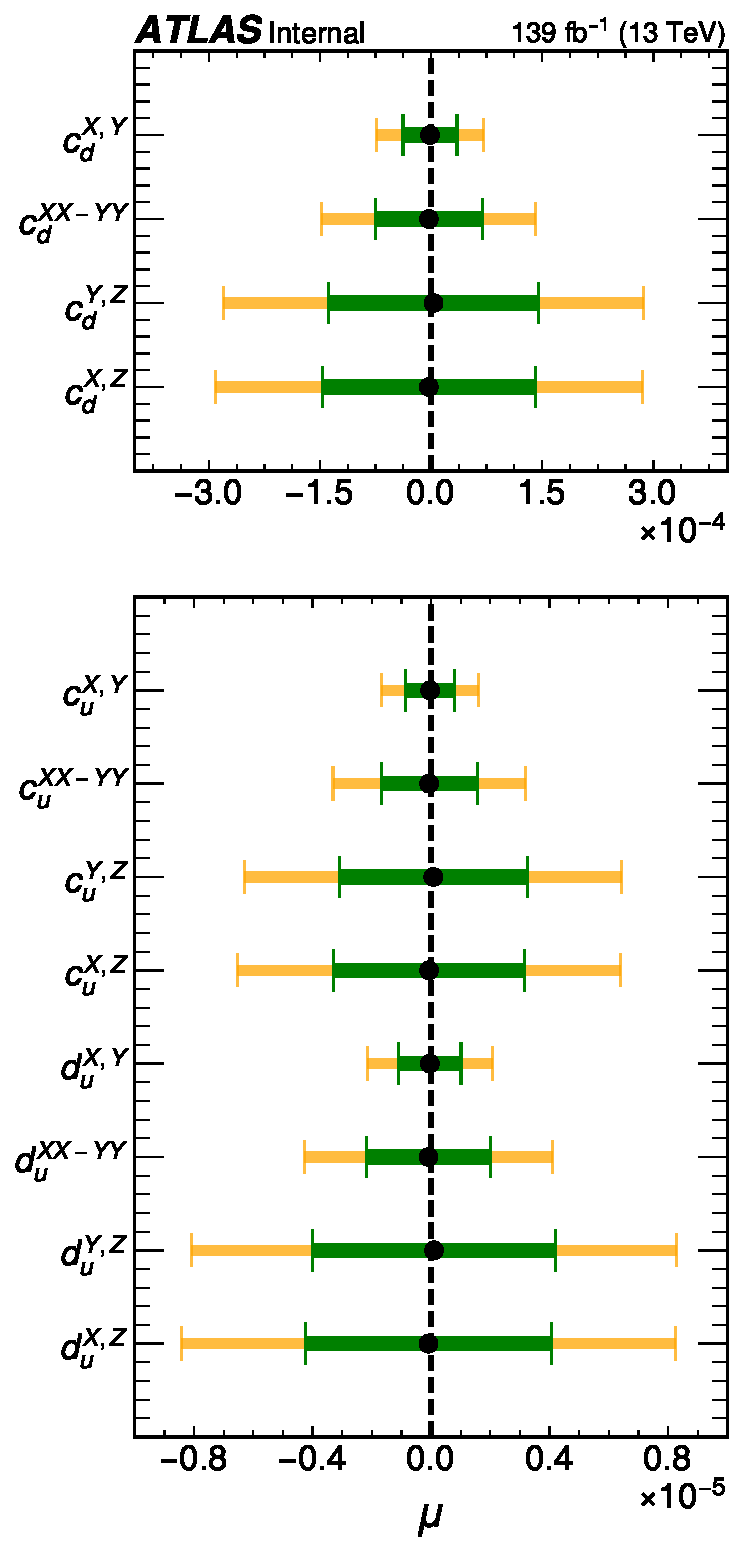
\includegraphics[width=0.4\textwidth]{figs/FMC_sys/SigFit_summary_AllSamples_muShift_m1} 
\caption{ Comparison of the fit results with average pileup $<\mu>$ increased and decreased by 1; left (+1) and right (-1). Results are obtained from 1000 toy datasets corresponding to four years of Run 2 luminosity. The X-axis is the sidereal phase, $\omega T$.
}
\label{fig:FMC_variation_summary}
\end{figure}




%\subsection{Residual systematic effects} %% the biases that we observe in chapter 5
\label{lab:Syst_ResidualEffecte}

%* 1. Discuss scambled toy studies.
%   Why we expect the average fit result to be zero,
%   indead we observed it consistent with zero in toy sutdies.
In Section~\ref{app:toys_signal_injected_scrambled} we tested our scrambled method on
our toy samples. The toys consist of SM-like toys (No signals), and 
signal-injected toys. In sidereal phase, the MS-like toys show data points
are distributed according to only statistical fluctuation. The signal injected toys show 
some oscillations correspond to injected signal shape.

The figure~\ref{fig:SM_like_toy_scrambled} shows a comparison of a SM-like toy before (left) and
and after scrambled (right). We can see that the scrambled toy is just like an original one,
it's also SM-like toy. In the same way we tested the scrambling on 1000 SM-like toys. 
The figure~\ref{fig:SM_like_toy_fit_results12} shows average of 1000 fitted results and their one/two 
sigma standard deviation. The left plot shows the results from SM-like toys before scrambling,
and the right plot shows the results after apply scrambling.
As we expected, in both case, average fit result on each coefficeint is in a good 
agreement with zero. Because, in SM-like toy datasets we have only 
simulated statistical uncertainties. Therefore, we expect no bias 
(average fit result consistent with zero).

In signal injected case, scrambling can completely washed the injected singal. 
The figure~\ref{fig:signal_injected_toy_p003_beforeAfter_scramble} show the compareson 
of before and after scrambling of an siganl injected toy sample. In the left plot we clearly 
see the oscillation pateren, but in the right plot after scrambling we didn't observe presence 
of any signals. After scrambing the fitted signal strength down to $-4.4E^{-7}\pm 3.8E^{-6}$;
 it was $5.3E^{-5}\pm 3.8E^{-6}$ before scrambling. This study concluded that event 
 if a singal is present the scrambling can wash it.
Also, if a dataset has only statistical uncertaity (e.g other systematics effects are negligible),
we can still expect that the fitted signal strength after scrambling will be 
consistent with zere (e.g no bias will be seen).



%* 2. Discuss the scrambled results from partially unblinded data.
%   We have observed the average fit results in several coefficients
%   diviate from zero at the order of one(or less) STD level. This is
%   different than what we learned from toy studies.
However, when we check the data using scrambling (partially unblind), we observe 
that average values of fit results in some singal strengths (coefficents) deviate 
from zero (bias). This can be clearly seen in figure~\ref{fig:real_data_scrambled_summary_combined}
where Run 2 - combined fit results are presented. In the plot, each black dot is an average fit results 
of 1000 scrabled datasets. In a few coefficents we observed the average fit results deviate from zero
but still within one sigma range. The exact numbers can be read from the table~\ref{table:scrambel_results_ll}.
This kind of deviation indicate that there is a systematic effact other than statisticle fluctuation. 
Because, as we expected from our toy studies we discussed before, if the statistical fluctuation is the 
only source of uncertainty then we should observe results from scrambled dataset also consistent with zero.

%* 3. The difference between the average fit result and zero (zero is
%    the theory expectation) in each coefficient can be a measurement of
%    spurious signal uncertaity. 
The deviation from zero in each coefficeint shown in figure~\ref{fig:real_data_scrambled_summary_combined} can be seen
as size of spurious signal uncertainty for corresponding coefficent.
 The spurious signal is models as Gaussian distribution centered at zero and it standard deviation
  is absolute values of average fit results (size of the deviation from zero) shown in figure~\ref{fig:real_data_scrambled_summary_combined}.
  The size of spurious signals for Run 2 fit and Run 2 - combined fit are given in table~\ref{table:spurious_signal_ll}.
  

% Sys table
%%%%%%%%%%%%%%%
%%ee+uu channel%%%
%%%%%%%%%%%%%%%
\begin{table}[hp]
  \begin{center}
  %%\resizebox{\textwidth}{!}{
  \begin{tabular}{|l|c| c| c| c |c|}
  \hline
   & Run2 & Run2-Comb. Fit \\
  \hline
  $d_{\it u}^{\it X,Z}$   & -3.23e-06 & -2.99e-06  \\
  \hline
  $d_{\it u}^{\it Y,Z}$   & -1.69e-06  & -2.5e-06  \\
  \hline
  $d_{\it u}^{\it XY,XY}$ & 8.03e-07  & -2.39e-07  \\
  \hline
  $d_{\it u}^{\it X,Y}$  & 3.21e-07  & 1.41e-07  \\
  \hline
  $c_{\it u}^{\it X,Z}$  & -2.51e-06  & -2.32e-06 \\
  \hline
  $c_{\it u}^{\it Y,Z}$  & -1.32e-06  & -1.94e-06  \\
  \hline
  $c_{\it u}^{\it XY,XY}$ & 6.24e-07  & -1.86e-07  \\
  \hline
  $c_{\it u}^{\it X,Y}$  & 2.50e-07  & 1.09e-07 \\
  \hline
  $c_{\it d}^{\it X,Z}$  & -1.12e-04  & -1.03e-04 \\
  \hline
  $c_{\it d}^{\it Y,Z}$  & -5.86e-05 & -8.66e-05  \\
  \hline
  $c_{\it d}^{\it XY,XY}$  & 2.78e-05 & -8.27e-06 \\
  \hline
  $c_{\it d}^{\it X,Y}$ & 1.11e-05 & 4.86e-06 \\
  \hline
  \hline
  \end{tabular}
  \end{center}
  \caption{
  Size of spurious signal uncertainties in $ee+\mu\mu$ channel, for Run 2 fit (first column) 
  and Run 2 - combined fit (second column, obtained from 10K samples).
  }\label{table:spurious_signal_ll}
  \end{table}

%%% Copy profiled X2 fit to here?






%\subsection{Statistical analyses including systematics}
\label{lab:Syst_stat}


\subsubsection{ Profiled $\chi^{2}$ with the spurious signal uncertainty}

We can include a spurious sisgnal uncertainty, $s$ to the 
$\chi^{2} = \sum \left(\frac{y_{i} - f_{i}(\mu)}{\sigma_{i}}\right)^{2}$ fit by replacing 
$f(\mu)$ with $F(\mu, \beta*s)$. Where $\beta$ is a nuissance parameter coinstrained by a 
normal Gaussian $N(0,1)$, and $s$ is the size of spurious signal uncertainty. We consider spurious singal
uncertainty is symmetric. For the siganl shpape $d_{u}^{X,Z}$ 
we can write $F(\mu, \beta*s)$ as
 $F_{d,u}^{X,Z}(\mu, \beta*s_{u}^{X,Z}) = 1+(\mu+\beta*s)*(6.28069*cos(x)-41.0569*sin(x))$.
 Then the total $\chi^{2}$ is
  $\chi^{2} = \sum \left(\frac{y_{i} - F_{u,i}^{X,Z}(\mu, \beta*s)}{\sigma_{i}}\right)^{2} + \beta^{2}$.
  Where $i$ is bin index, the $\beta^{2}$ is due to the normal Gaussian constaint of $\beta$.


The figure~\ref{fig:real_data_scrambled_Spurious_signal} shows fit results from profiled $\chi^{2}$ 
with a spurious signal uncertainty $s_{u}^{X,Z} = 3.01e-06$. In the left plot,
 we fit a scrabked dataset. In the right plot, we fit a singal injected toy dataset. In both case, including 
 spurious signal uncertainty enlargened the final fit uncertainty by 
 29\% (28\% for the singal injected toy dataset). 
 The figure~\ref{fig:signal_injected_toy_single_dataset} show the signal injected toy dataset.
 The injected singal amplitude is $\sigma_{LIV}/\sigma_{SM}=0.0009$.


\begin{figure}[ht]
    \centering
    
\includegraphics[width=0.45\textwidth]{figs/partially_unblinded_results/profile_chi2_shape_sys_du_XZ.pdf}
    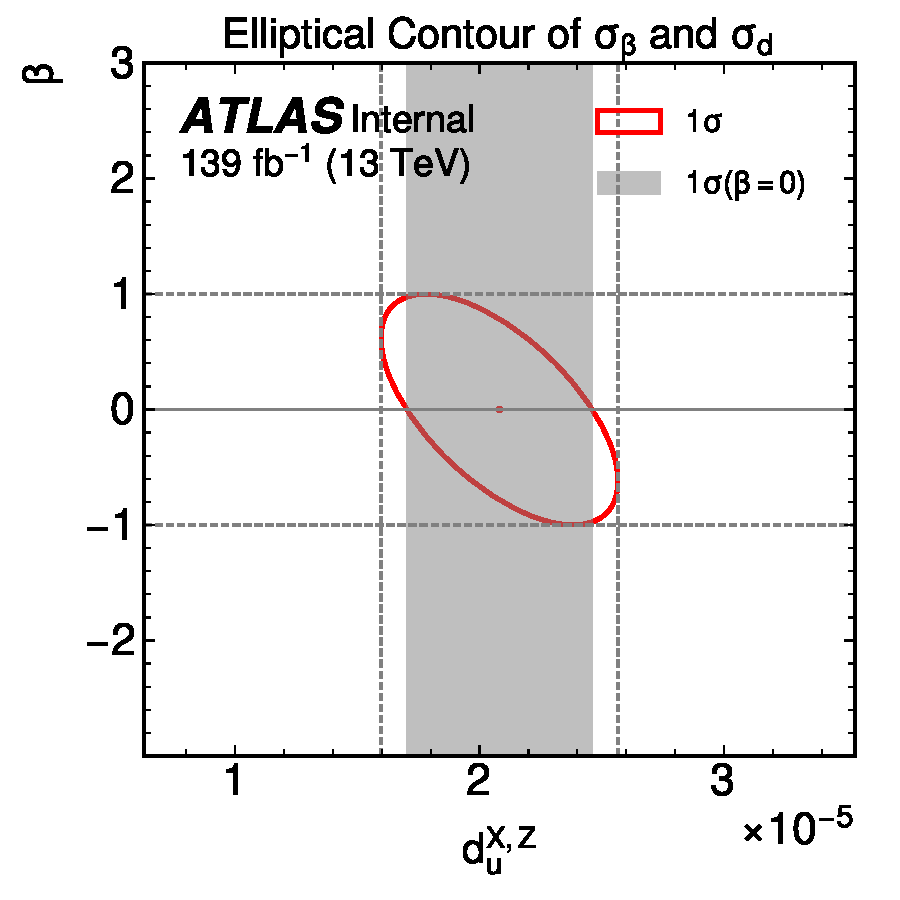
\includegraphics[width=0.45\textwidth]{figs/partially_unblinded_results/profile_chi2_shape_sys_du_XZ_sig0009.pdf}
    
    \caption{Combined fit results of profiled $\chi^{2}$ fit, which includes the spurious
     signal uncertainty as a nuisance parameter $\beta$. The left plot is the result 
     from one of the scrambled datasets. The right plot is a signal-injected toy dataset
      with strength $\sigma_{LIV}/\sigma_{SM}=0.0009$; the signal model is $d_{u}^{X,Z}$. 
    The grey band is the 68\% uncertainty band without spurious signal. The fit uncertainty
     is 29\%(28\% for the toy) larger when we add the spurious signal uncertainty to the fit.}
    \label{fig:real_data_scrambled_Spurious_signal}
\end{figure}
    
    
\begin{figure}[ht]
    \centering
    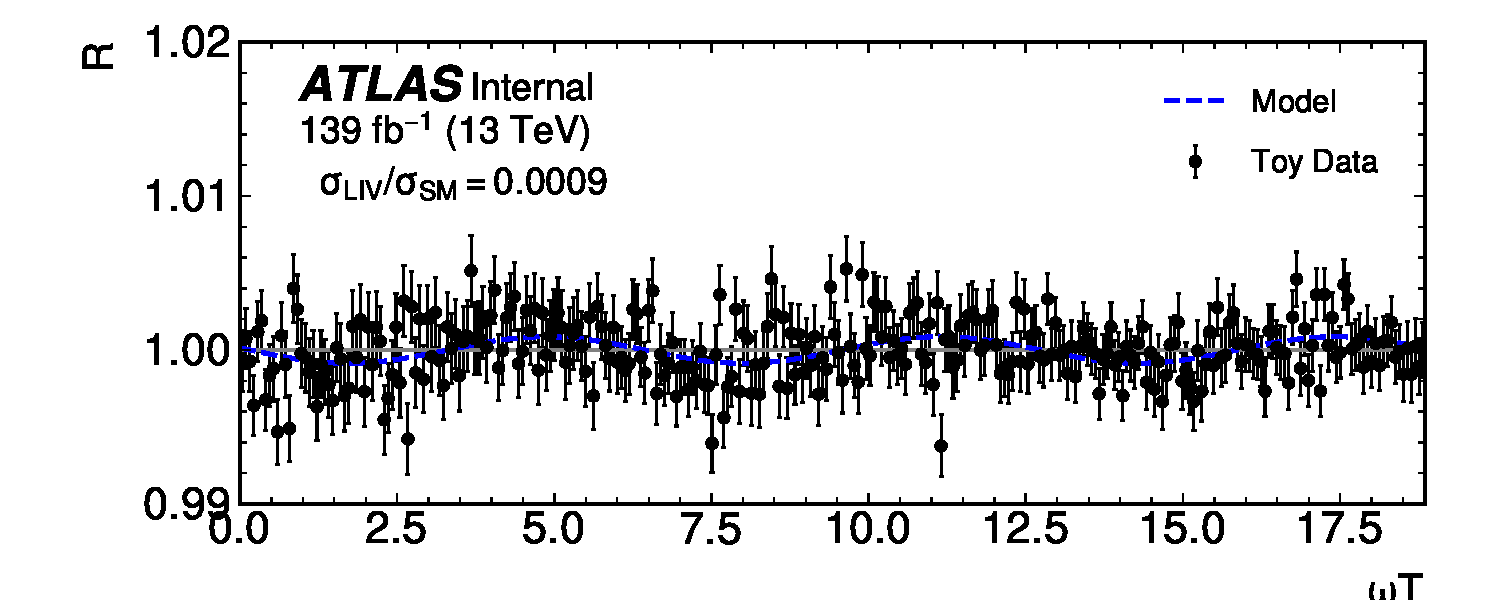
\includegraphics[width=0.90\textwidth]{figs/partially_unblinded_results/profile_chi2_toy_du_XZ_postfit_sig0009.pdf}
    
    \caption{The signal-injected combined toy dataset with signal amplitude
     $\sigma_{LIV}/\sigma_{SM}=0.0009$ and  $d_{u}^{X,Z}$ model (post-fit).
      The blue line is the signal shape after the combined fit. The  error
       bars on the data points are statistical errors.}
    \label{fig:signal_injected_toy_single_dataset}
\end{figure}





\subsection{Summary of results}
\label{lab:Syst_result}

%\subsection{Scan periods with spurious signal uncertainties included}
\label{sec:scan_periods_sys}
%%% show significance plot
%%% show fit uncertainties
The significance of injected signals is studied as a function of probing
periods using signal-injected toys. We performed this study using four
types of SME signal shapes, and the injected maximum signal amplitude
for each type of signal is 5\%.  The injected SME signal shapes are
$d_{u}^{X,Z}$, $d_{u}^{Y,Z}$, $d_{u}^{XX-YY}$, $d_{u}^{X,Y}$.

The top left plot in Figure~\ref{fig:scan_period_toy_Sys_combined_fit}
shows the canned significance without systematic included in the fit. As we expected, a huge spike appeared when
the probing period was equal to the sidereal period (23:56:04) because
the signal is injected in the sidereal period.
The top right plot shows the significance with systematic included 
in the fit. The significance is reduced when we add systematics. 
Profiled $\chi^{2}$ fit with systematics does not change the value
of parameters obtained from the fit, as shown in the bottom left plot.
The main contribution of the systematics is in the fit uncertainties. 
The bottom right plot shows the ratio of the fit uncertainties 
with/without systematic inclusion in the fit. The fit uncertainties
are increased; for example, 12.5\% increased in $d_{u}^{X,Z}$ signal shape. 
The impact of a systematic mainly depends on the input size. The corresponding spurious signal systematic are listed in the table~\ref{table:real_data_scrambled_Generic_combined_fit}



\begin{figure}[!ht]
\centering
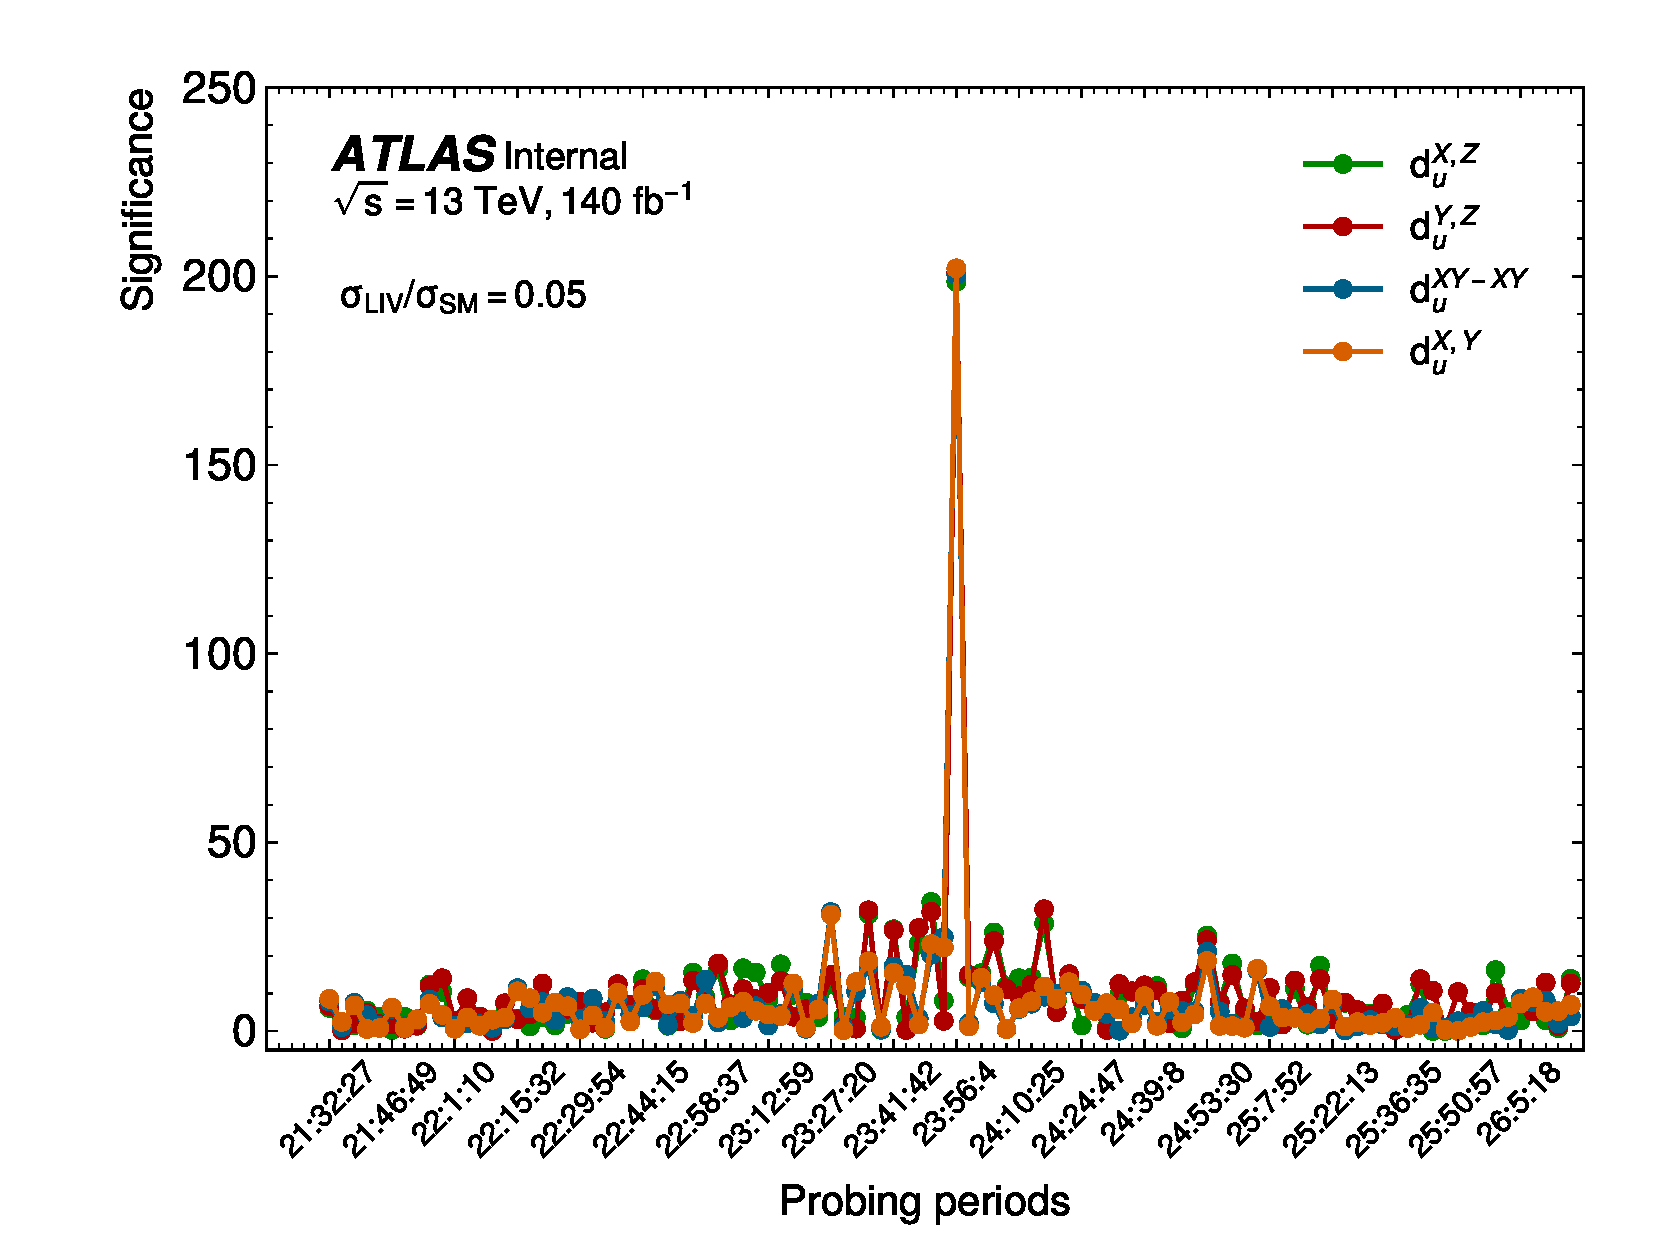
\includegraphics[width=0.45\textwidth]{figs/partially_unblinded_results/scan_periods/scan_significance_toys}
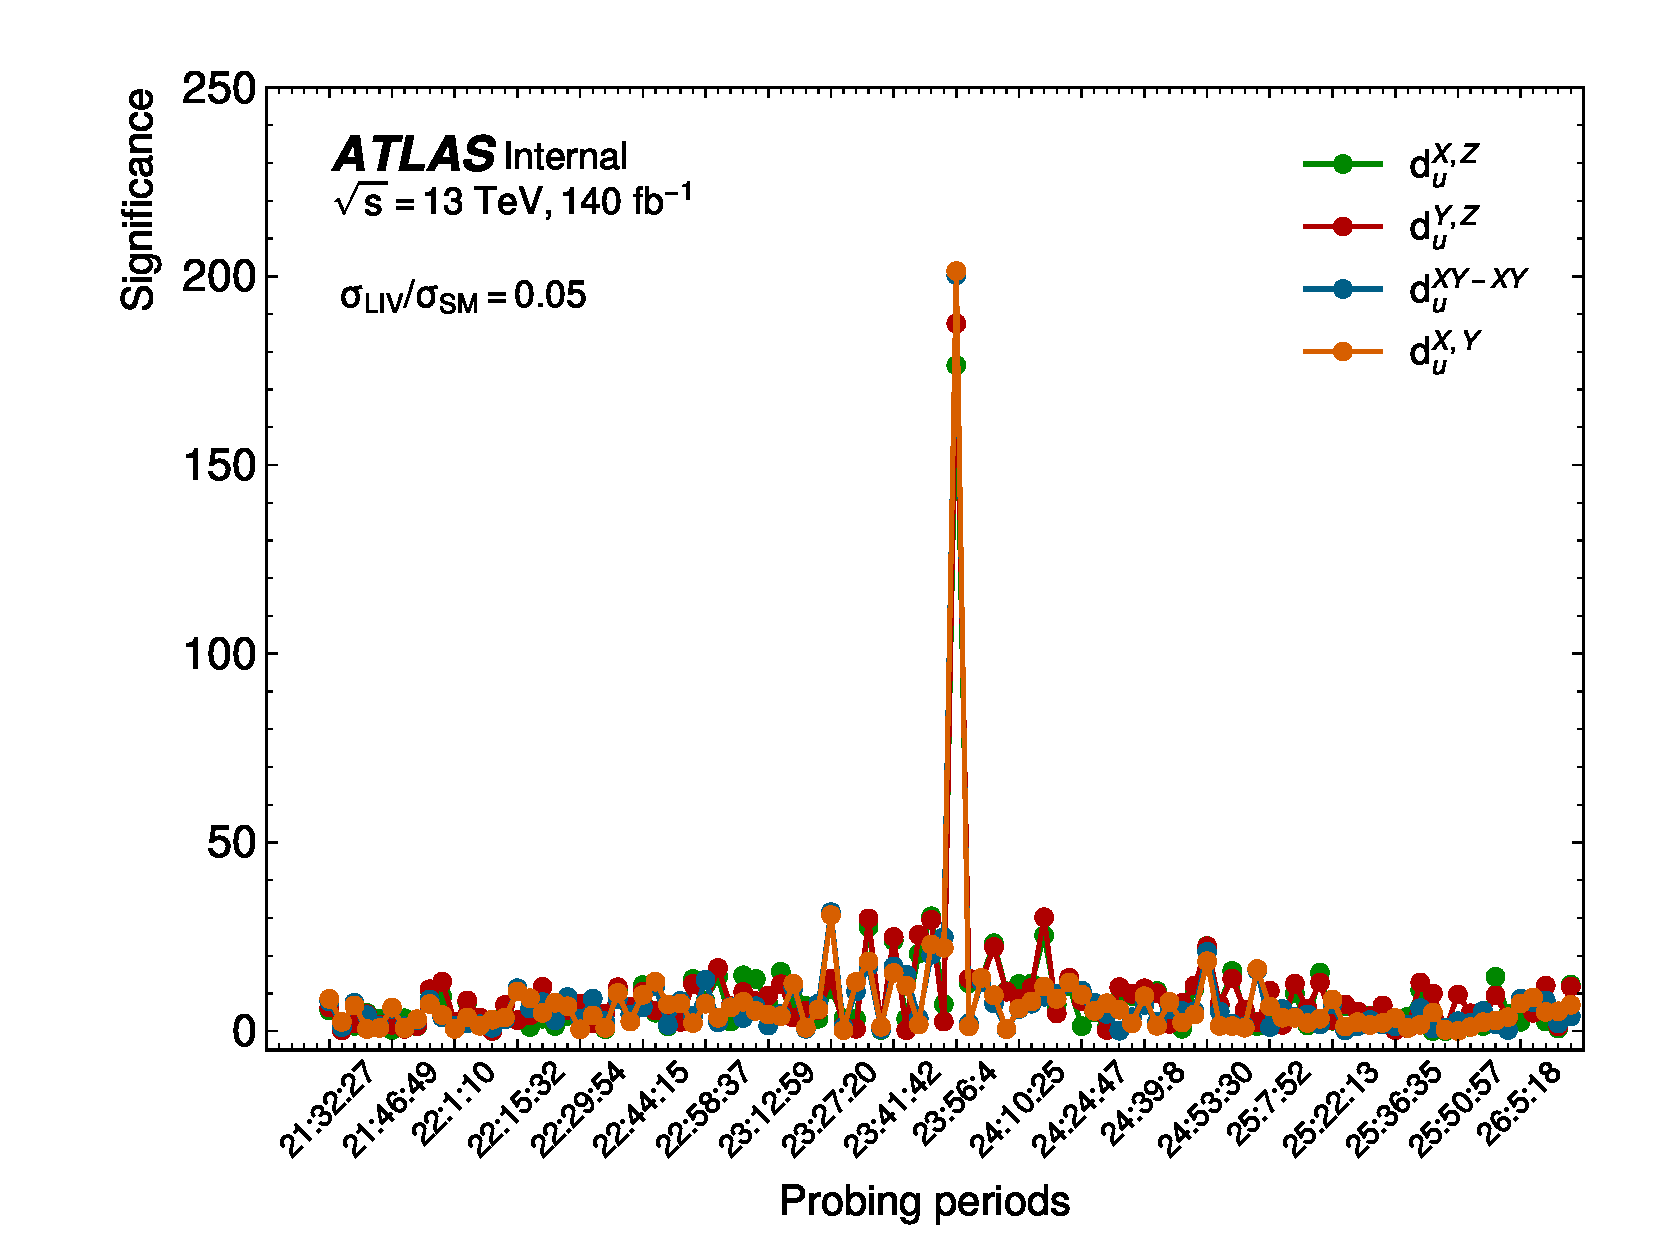
\includegraphics[width=0.45\textwidth]{figs/partially_unblinded_results/scan_periods/scan_significance_toys_with_Sys}\\
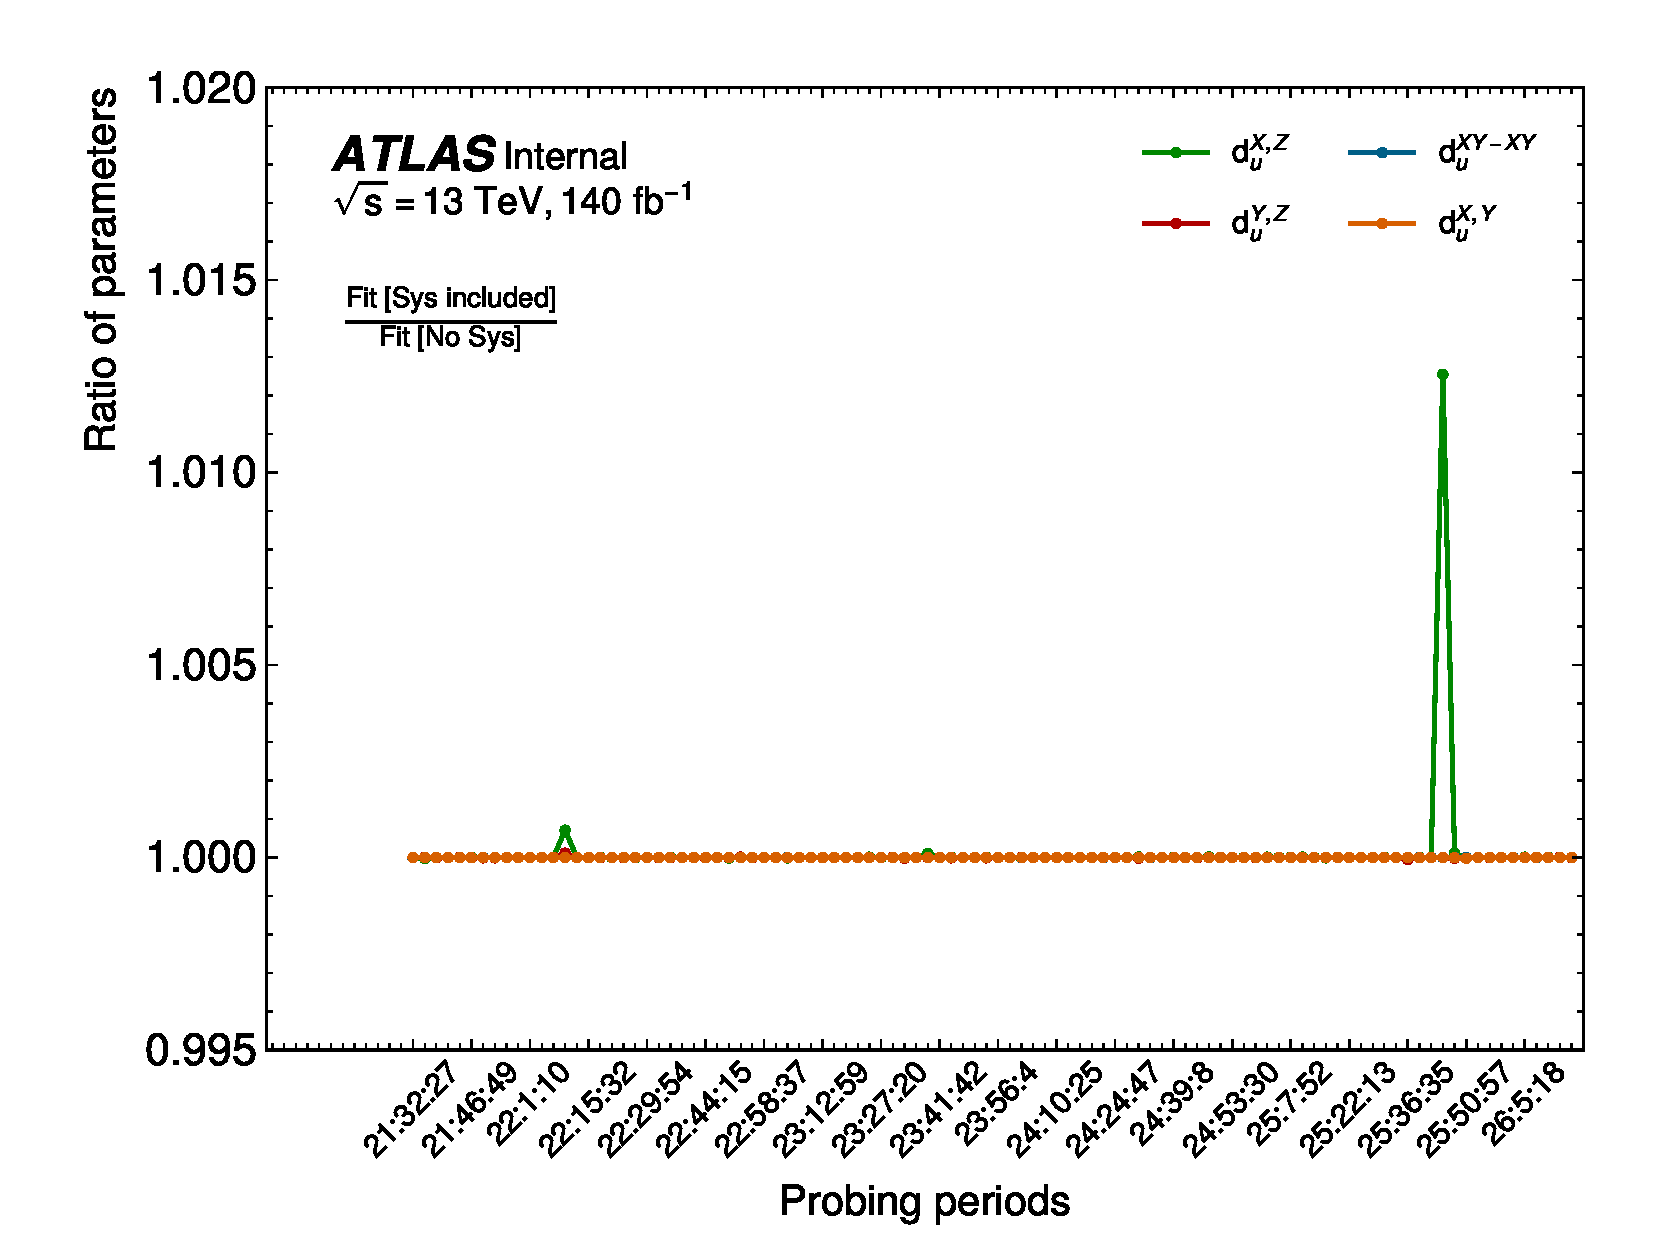
\includegraphics[width=0.45\textwidth]{figs/partially_unblinded_results/scan_periods/scan_significance_toys_Ratio_of_Fits}
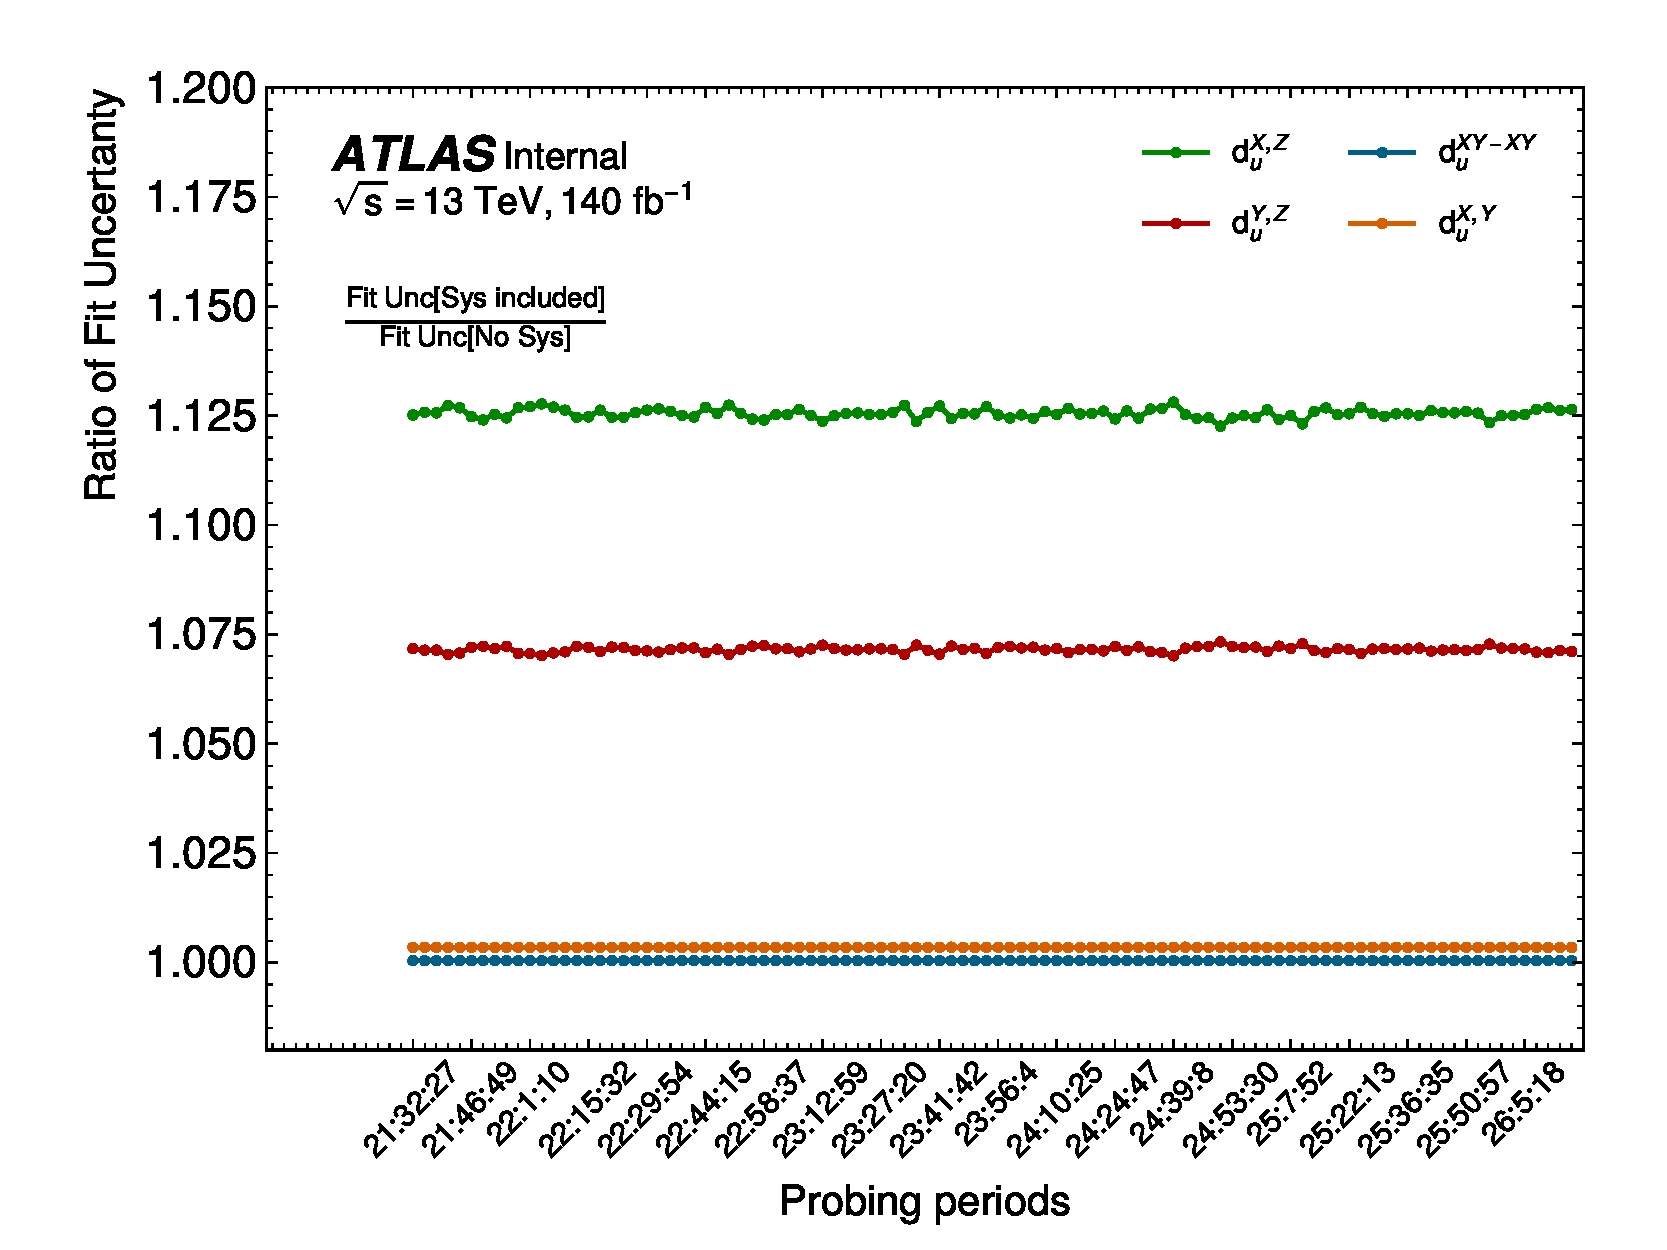
\includegraphics[width=0.45\textwidth]{figs/partially_unblinded_results/scan_periods/scan_significance_toys_impact_of_Sys}
\caption{Scan probing periods on the signal-injected toys. Four types of SME signal shapes are injected at maximum amplitude 5\% level, as shown in the plots. The top left plot shows significance without systematic is included in the fit. The Top right plot shows significance with systematic included in the fit. The bottom left plot shows the ratio of fitted parameters with/without systematic included in the fit. The bottom right plot shows the ratio of the fit uncertainties with/without systematic inclusion in the fit.}
\label{fig:scan_period_toy_Sys_combined_fit}
\end{figure}

\clearpage 
\section{Model independent limits}
\label{sec:Scrambling_generic_limits}
%%%%%%%
%% Generic model
%%
\subsection{Model-independent signal shapes}
\label{sec:generic_models}

The SME predicts $n$th-order sinusoidal temporal oscillations of the forms
$\cos(n\omega_\oplus T_\oplus)$ and $\sin(n\omega_\oplus T_\oplus)$. Recall
from Sec.~\ref{ssec:SME} that a dimension $d$ SME operator is multiplied
by a coefficient of dimension $4-d$. A given coefficient induces a tower of 
$n$-order sidereal harmonics $n\omega_\oplus T_\oplus$ 
the number of Lorentz indices of an SME coefficient. 
For example, revisiting again ${\cal L}_b$ from Eq.~\eqref{bterm},
the SME coefficient $b_\mu$ has one Lorentz index. We showed 
in Eq.~\eqref{ATLAScomps} that only $n=1$ and 
$\cos(\omega_\oplus T_\oplus), \sin(\omega_\oplus T_\oplus)$ appear. 
For the $c$- and $d$-type coefficients, with two Lorentz indices, 
we expect $n=1$ and $n=2$ harmonics. This is observed in the 
decomposition of $c_f^{33}$ in Eq.~\eqref{c33}. 
Note that unique linear combinations of SME coefficients (prefactors) are
associated to a single harmonic of order $n$~\cite{Kostelecky:2009zp}.
There are no ``cross terms"
involving, for example, a prefactor with time-dependent
behavior controlled by both $\cos(\omega_\oplus T_\oplus)$ 
and $\cos(2\omega_\oplus T_\oplus)$. This is a generic
result applying for all $n$.

For the $a^{(5)}$- and $b^{(5)}$-type coefficients 
one finds $n=1, 2$ and $3$ harmonics in general.
The $a^{(5)}$ predictions for the Drell-Yan cross section
evaluated in the ATLAS detector frame are found to be absent 
$3\omega_\oplus$ signatures. This contrasts with 
the cross section for deep inelastic scattering, 
where all harmonics appear.
An intuitive explanation for this 
absence is that Drell-Yan is
a more colliear or ``symmetric" process 
than deep inelastic scattering.
As a result, fewer coefficient components 
are present in the detector-frame
cross section. The ones that do appear have 
laboratory indices which, upon replacing with the SCF coefficients,
exhibit only first and second harmonics.
This is likely to be a special case
rather than a generic expectation for Drell-Yan.
A significant number of nonminimal 
SME coefficients of low mass 
dimension (e.g. $d=5,6$) have distinct
symmetry properties relative to those exhibited by
the $a^{(5)}$-type coefficients. 
Anticipating that phenomenological predictions
with higher than $2\omega_\oplus$ harmonics
will appear in future provides motivation 
for developing the generic framework outlined here.

In this section, we outline a new method for capturing
higher-order harmonics that encompass 
any new physics associated with sidereal oscillations. 
While the SME is a model-independent effective field theory, it makes
specific predictions about the prefactors multiplying the 
sidereal functions. We generalize these types of signal shapes
by leaving the prefactors as free fit parameters. 

In particular, we consider three distinct generic 
model signal shapes 
%
\begin{subequations}
\label{eq:generic_shapes}
\begin{align}
    f_{1}(\omega_\oplus T_\oplus| p_{1}, p_{2}) 
    &= 1+ p_{1}
    \cos(\omega_\oplus T_\oplus) 
    + p_{2}\sin(\omega_\oplus T_\oplus), \label{eq:generic_shape1} \\
    f_{2}(2\omega_\oplus T_\oplus| p_{1}, p_{2}) 
    &= 1+ p_{1}\cos(2\omega_\oplus T_\oplus) 
    + p_{2}\sin(2\omega_\oplus T_\oplus), \label{eq:generic_shape2} \\
    f_{3}(3\omega_\oplus T_\oplus| p_{1}, p_{2}) 
    &= 1+ p_{1}\cos(3\omega_\oplus T_\oplus) 
    + p_{2}\sin(3\omega_\oplus T_\oplus), \label{eq:generic_shape3}
\end{align}
\end{subequations}
%
and treat each function $f_1, f_2$ and $f_3$ with prefactor parameters
$p_1$ and $p_2$ as mutually exclusive. As we limit
attention to a finite number of free parameters, and make no assumption 
about the physics generating them, we refer to them as ``generic models". 
Parameters $p_1$ and $p_2$ are to be determined from $\chi^{2}$
fits to data. The results of these fits are the parameter values and a covariance matrix.
The corresponding $p_1$ and $p_2$ confidence intervals are obtained
from the covariance matrix.

%%% Should I write chi2 fits?
%Unlike SME models, the generic model has two free parameters to be determined 
%from fit to data by applying two parametric $\chi^{2}$ fits. The fit result 
%would be values $p_{1}$, $p_{2}$ and covariance matrix. Confidence interval 
%for $p_{1}$ and $p_{2}$ are obtained from the corresponding covariance matrix.


\subsection{Spurious signal uncertainties on $p_{1}$ and $p_{2}$}
%%% fit to 10K scrambled datasets.
%%% fit results

Figure~\ref{fig:real_data_scrambled_Generic_combined_fit} shows the estimated 
set of parameters, $p_{1}$ and $p_{2}$, corresponding to generic models with 
different frequencies, 
$\omega_\oplus T_\oplus$, $2\omega_\oplus T_\oplus$, 
$3\omega_\oplus T_\oplus$. These results 
are obtained from 10000 scrambled datasets by fitting each dataset with 
the generic signal shapes. 
The three signal shapes are mutually exclusive, 
so a fit includes one signal shape at a time. 
The corresponding numerical values 
of the Fig.~\ref{fig:real_data_scrambled_Generic_combined_fit} are also given 
in the Tab.~\ref{table:real_data_scrambled_Generic_combined_fit}.

In the ideal case, 
we could expect the central value of the parameters to be zero
because we took an average of the 10000 fit results from the scrambled datasets.
In reality, the average values are not zero, as we have seen in
Fig.~\ref{fig:real_data_scrambled_Generic_combined_fit}.  
Therefore, we can take 
these non-zero values as spurious signal 
uncertainties and include them in the unblinded results.

\begin{figure}
\centering
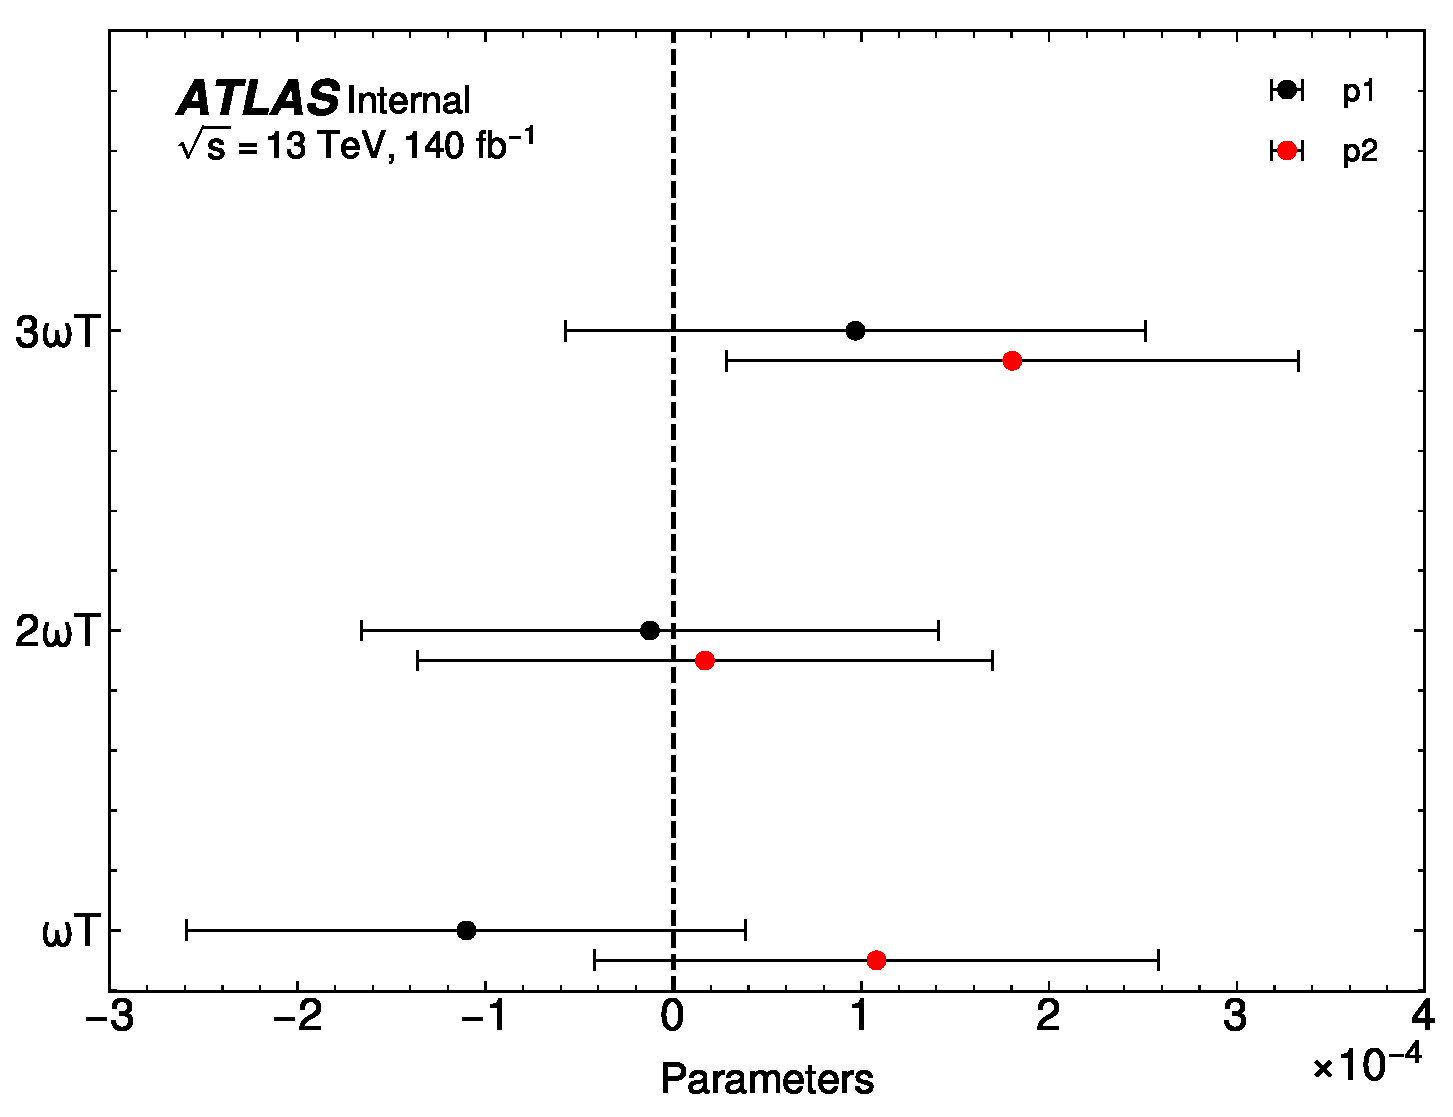
\includegraphics[width=0.75\textwidth]{figs/partially_unblinded_results/sig_config_6013_sidereal_combined_SciPy_generic}
\caption{Estimated parameters and their 
uncertainties of generic signal shapes; 
obtained by fitting 10000 scrambled datasets. 
The plot shows the mean and 
one standard deviation of 10000 fit results.
Note $\omega T = \omega_\oplus T_\oplus$ on the $y$-axis.}
\label{fig:real_data_scrambled_Generic_combined_fit}
\end{figure}

%%%%
%%% Sys table
%%%%
%%%%%%%%%%%%%%%
%%ee channel%%%
%%%%%%%%%%%%%%%
\begin{table}[hp]
\begin{center}
\color{gray}
%\resizebox{\textwidth}{!}{
\begin{tabular}{|l|c| c| c|}
\hline
  & \multicolumn{3}{|c|}{Generic models}\\
\hline
 Pars & $\omega_\oplus T_\oplus$ & $2\omega_\oplus T_\oplus$ & $2\omega_\oplus T_\oplus$\\
 \hline
$p_{1}$ & -1.10e-04 $\pm$ 1.49e-04 & -1.25e-05 $\pm$  1.54e-04 & 9.69e-05 $\pm$  1.54e-04\\
\hline
$p_{2}$ & 1.08e-04 $\pm$ 1.50e-04 & 1.68e-05 $\pm$ 1.53e-04 & 1.80e-04 $\pm$ 1.52e-04\\
\hline
\hline
\end{tabular}
%}
\color{black}

%\resizebox{\textwidth}{!}{
\begin{tabular}{|l|c| c| c|}
  \hline
    & \multicolumn{3}{|c|}{Generic models}\\
  \hline
   Pars & $\omega_\oplus T_\oplus$ & $2\omega_\oplus T_\oplus$ & $2\omega_\oplus T_\oplus$\\
   \hline
  $p_1$ & $(-1.23 \pm 1.49)\times 10^{-4}$ & $(-0.25 \pm 1.54)\times 10^{-4}$ & $(0.84 \pm 1.54)\times 10^{-4}$ \\
  \hline
  $p_2$ & $(1.08 \pm 1.50)\times 10^{-4}$ & $(0.16 \pm 1.53)\times 10^{-4}$ & $(1.79 \pm 1.52)\times 10^{-4}$ \\
  \hline
  $\text{corr}(p_1,p_2)$ & $0.0014$ & $-0.00086$ & $0.0071$ \\
  \hline
  \hline
  \end{tabular}
 % }
\end{center}
\caption{Estimated parameters and their 
uncertainties of generic signal shapes; 
obtained by fitting 10000 scrambled datasets. 
The means and one standard deviation of the 10000 fit results.}
\label{table:real_data_scrambled_Generic_combined_fit}
\end{table}
%

\subsection{Profiled $\chi^{2}$ fit with generic models}
% introduce spurious signal uncertainty size, s1 and s2
% introduce normal gaussian nuisance, b1, b2
% F(x, p1, p1,| b1, b2) = f(x, p1+b1*s1, p2+b2*s2)
Here we introduce, $s_{1}$ and $s_{2}$ 
as size of spurious signal uncertainties
corresponds to the parameters 
$p_{1}$ and $p_{2}$. The values of $s_{1}$ and 
$s_{2}$ are the absolute values of 
$p_{1}$ and $p_{2}$ in the 
Table~\ref{table:real_data_scrambled_Generic_combined_fit}, 
as these values are obtained from scrambled 
datasets (we take these samples as signal-free datasets). 

To add spurious signal uncertainties to the $\chi^{2}$ fit, 
we rewrite the Eqs.~\eqref{eq:generic_shapes} as
\begin{equation}
F(\omega_\oplus T_\oplus,\ p_1,\ p_2| \beta_{1},\ \beta_{2}) 
= f(\omega_\oplus T_\oplus,\ p_1+\beta_{1}*s_1, \ p_2+\beta_{1}*s_2), 
\end{equation}
where $\beta_{1}$ and $\beta_{2}$ nuisance parameters constrained as they
follow normal Gaussian centered at zero, 
and the standard deviation is one. 
$s_{1}$ and $s_{2}$ are constant in the equations.
The profiled $\chi^{2}$ fit is constructed using the function 
$F(\omega_\oplus T_\oplus,\ p_1,\ p_2| \beta_{1},\ \beta_{2})$. 




\subsection{Application of generic results}

In this subsection we show that the 
model-independent constraints in 
Eqs.~(\ref{eq:generic_shape1}--\ref{eq:generic_shape3}), 
together with the theory predictions given in 
Sec.~\ref{subsec:WC} 
(see Eqs.~(\ref{eq:SME coefficient functions}-\ref{eqn:14})) 
allow to reproduce the results of the 
one-parameter fits presented in Table~\ref{table:scrambel_results_10K}.

The starting point are the model-independent 
fits for the parameters $(p_1,p_2)$ summarized in 
Table~\ref{table:real_data_scrambled_Generic_combined_fit}. 
Adopting a simple frequentist $\chi^2$ fit 
based on the theoretical expressions in 
Sec.~\ref{subsec:WC} we obtain the 
results in Table~\ref{table:Direct_vs_Indirect_Comparison}, 
where, for ease of comparison, we show 
direct and indirect determinations side 
by side (the former are taken directly from 
Table~\ref{table:scrambel_results_10K}).

We see that the two procedures yield perfectly compatible results. 
Figure~\ref{fig:direct_indirect_results} shows the direct and indirect
 results in a plot for visualization.

\begin{table}[hp]
  \begin{center}
%  \resizebox{\textwidth}{!}{
  \begin{tabular}{|l|c|c|}
    \hline
    \hline
    Parameters & Direct & Indirect \\
    \hline
    $d_{\it u}^{\it X,Z}$ & $-(2.99 \pm 3.62)\times 10^{-6}$& $-(3.02 \pm 3.62)\times 10^{-6}$ \\
    \hline
    $d_{\it u}^{\it Y,Z}$ & $-(2.50 \pm 3.59)\times 10^{-6}$ & $-(2.55 \pm 3.59)\times 10^{-6}$\\
    \hline
    $d_{\it u}^{\it XY,XY}$ & $-(0.24 \pm 1.89)\times 10^{-6}$ &  $-(0.24 \pm 1.89)\times 10^{-6}$\\
    \hline
    $d_{\it u}^{\it X,Y}$ & $(1.41 \pm 9.40)\times 10^{-7}$ & $(1.40 \pm 9.41)\times 10^{-7}$\\
    \hline
    $c_{\it u}^{\it X,Z}$ & $-(2.32 \pm 2.81)\times 10^{-6}$ & $-(2.35 \pm 2.81)\times 10^{-6}$\\
    \hline
    $c_{\it u}^{\it Y,Z}$ & $-(1.94 \pm 2.79)\times 10^{-6}$ & $-(1.98 \pm 2.79)\times 10^{-6}$\\
    \hline
    $c_{\it u}^{\it XY,XY}$ &  $-(0.19 \pm 1.47)\times 10^{-6}$ &  $-(0.19 \pm 1.47)\times 10^{-6}$\\
    \hline
    $c_{\it u}^{\it X,Y}$ &  $(1.09 \pm 7.31)\times 10^{-7}$ & $(1.09 \pm 7.31)\times 10^{-7}$\\
    \hline
    $c_{\it d}^{\it X,Z}$ & $-(1.03 \pm 1.25)\times 10^{-4}$ &$-(1.05 \pm 1.25)\times 10^{-4}$ \\
    \hline
    $c_{\it d}^{\it Y,Z}$ & $-(0.87 \pm 1.24)\times 10^{-4}$ & $-(0.82 \pm 1.24)\times 10^{-4}$\\
    \hline
    $c_{\it d}^{\it XY,XY}$ & $-(0.83 \pm 6.54)\times 10^{-5}$ & $-(0.82 \pm 6.54)\times 10^{-5}$\\
    \hline
    $c_{\it d}^{\it X,Y}$ & $(0.49 \pm 3.25)\times 10^{-5}$ & $(0.49 \pm 3.26)\times 10^{-5}$ \\
    \hline
    \hline
    \end{tabular}
  %  }
  \end{center}
  \caption{Comparison between the direct 
  and indirect (using the results of the 
  two-parameter fits) extraction of 
  bounds on the $c$- and $d$-coefficients.}
  \label{table:Direct_vs_Indirect_Comparison}
  \end{table}
  %

  \begin{figure}[!h]
    \centering
    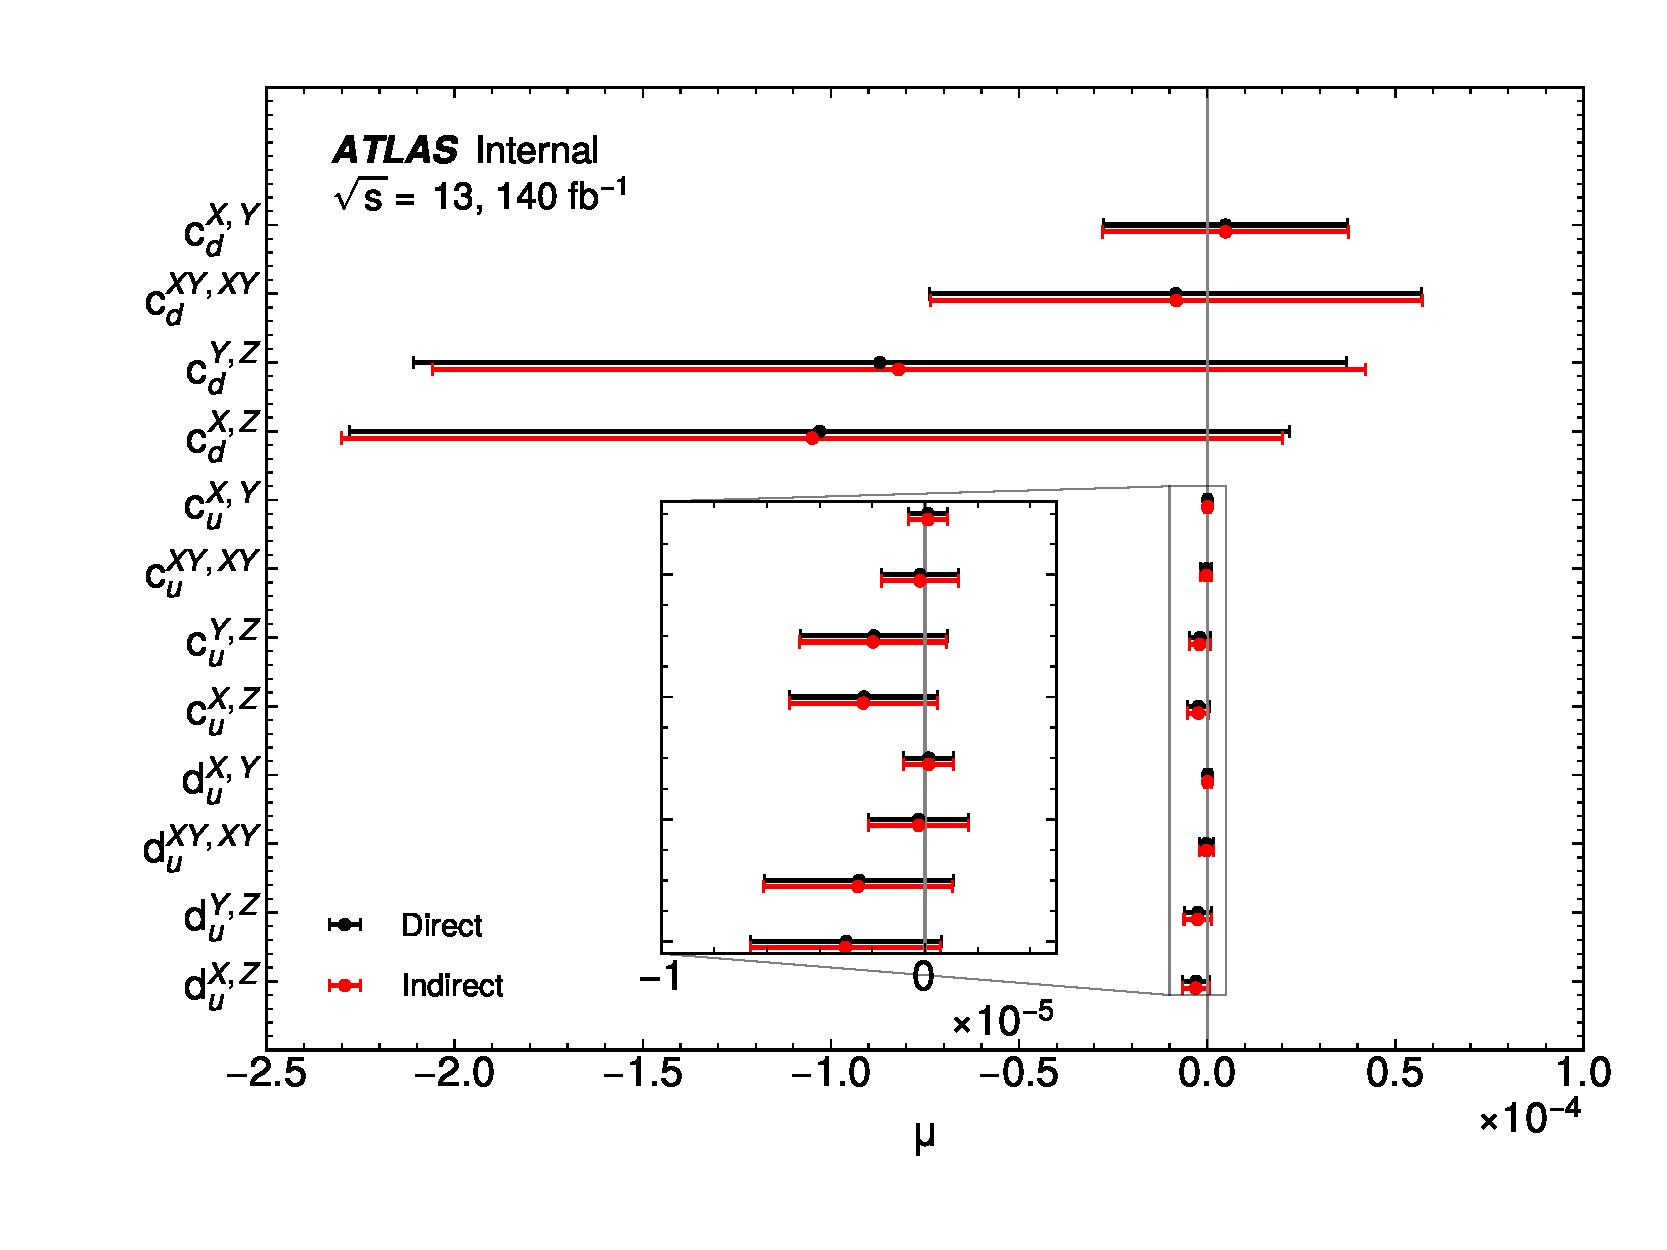
\includegraphics[width=0.75\textwidth]{figs/partially_unblinded_results/direct_indirect_test_results}
    \caption{
      Comparison of the direct (fit results of SME predictions) 
      and indirect (obtained using results of generic models).
      The indirect results are consistent with the direct results.
      Uncertainties correspond to 68\% (one-sigma) confidence intervals.
    }
    \label{fig:direct_indirect_results}
    \end{figure}
  

\subsection{Disentangling coefficient degeneracies}
\label{ssec:disentangle}

We briefly discuss the possibility of detecting a degenerate signal,
meaning one where at least two SME coefficients
could contribute to the signal.
Recall Eqs.~\eqref{eq:SME coefficient functions} and, for definiteness,
consider a scenario where the signal matches ``opposite phase" 
single-harmonic oscillations in the $u$-quark sector. 
For the minimal $c$- and $d$-type 
coefficients there are two possibilities:
\begin{align}
&d_u^{XZ}\left[6.28069\cos(\omega_\oplus T_\oplus)
-41.0569 \sin(\omega_\oplus T_\oplus)\right], \nonumber \\
&c_u^{XZ}\left[8.084\cos(\omega_\oplus T_\oplus)
-52.8451 \sin(\omega_\oplus T_\oplus)\right]
\end{align}
The small difference in magnitudes is a factor of 1.287.
Both coefficients can contribute to the signal, but 
a single measurement at $Q=m_Z$ can 
not distinguish between the possibilities: a $d_u$ dominated one, 
a $c_u$ dominated one, or some combination of the two.
A way to disentangle the signal 
is to perform another measurement at a different $Q$ value.
Referring to Fig.~\ref{fig:coeff_bounds}, one observes
that the $c_u$-type coefficient curve in red and
the $d_u$-type coefficient curve in green display distinct
patterns of sensitivity as $Q$ varies. 
The sensitivity to $c_u$ increases from around 
70 GeV and below, whereas $d_u$ 
decreases from $m_Z$ down to about 40 GeV. 
Focusing on the 40-45 GeV bin, the sensitivity
to $c_u$ decreases by about one order of magnitude, 
whereas $d_u$ about three orders of magnitude (both relative to $Q=m_Z$).
If the signal strengths measured at $Q=m_Z$ 
and $Q=40-45$\;GeV are found to differ by roughly an order of magnitude, 
this would disfavor the $d_u$-dominated scenario. This would suggest
that Lorentz violation couples more strongly 
to the $L+R$ chiral combination, which is the combination
that leaves the $u$-quark polarization properties unaffected.



\clearpage
\section{Unblinded data studies} %%  [Ablet/Enrico]
\label{lab:UnblindedDataStudy}
%\subsection{General method}
\subsubsection{95\% C.L. using scrambled data}
\subsubsection{Discovery limits}
\subsection{Data results - to come -}



\clearpage
\section{Result}
\label{sec:result}
Place your results here.

% All figures and tables should appear before the summary and conclusion.
% The package placeins provides the macro \FloatBarrier to achieve this.
% \FloatBarrier

\clearpage
\section{Interpretation}
\label{sec:interpretation}
You can find some text snippets that can be used in papers in \texttt{latex/atlassnippets.sty}.
To use them, provide the \texttt{snippets} option to \texttt{atlasphysics}.

\clearpage
\section{Conclusion}
\label{sec:conclusion}
Place your conclusion here.



%-------------------------------------------------------------------------------
% If you use biblatex and either biber or bibtex to process the bibliography
% just say \printbibliography here.
 \printbibliography
% If you want to use the traditional BibTeX you need to use the syntax below.
% \bibliographystyle{obsolete/bst/atlasBibStyleWithTitle}
% \bibliography{ANA-EXOT-2021-37-INT1,bib/ATLAS,bib/CMS,bib/ConfNotes,bib/PubNotes}
%-------------------------------------------------------------------------------

%-------------------------------------------------------------------------------
% Print the list of contributors to the analysis.
% The argument gives the fraction of the text width used for the names.
%-------------------------------------------------------------------------------
\clearpage
The supporting notes for the analysis should also contain a list of contributors.
This information should usually be included in \texttt{mydocument-metadata.tex}.
The list should be printed either here or before the Table of Contents.
\PrintAtlasContribute{0.30}

%-------------------------------------------------------------------------------
\clearpage
\appendix
\part*{Appendices}
\addcontentsline{toc}{part}{Appendices}
%-------------------------------------------------------------------------------

In an ATLAS note, use the appendices to include all the technical details of your work
that are relevant for the ATLAS Collaboration only (e.g.\ dataset details, software release used).
This information should be printed after the Bibliography.




\end{document}
